\documentclass[11pt]{book}
\usepackage[utf8]{inputenc}
%amsmath ma con meno errori
\usepackage{mathtools}
%altri pacchetti di ams
\usepackage{amsfonts, amssymb, amsthm}
%corsivo bello
\usepackage{mathrsfs}
%per le frazioni a riga fatte bene
\usepackage{xfrac}
%per le immagini
\usepackage{graphicx}
\graphicspath{{c:/Users/39349/OneDrive/Desktop/Sito/FrancescoMussin.github.io/AnalisiComplessa/AnalisiComplessaImmagini}}
%riduce i warning di hbox
\usepackage{microtype}
%immagini vettoriali e diagrammi commutativi
\usepackage{tikz}
\usetikzlibrary{shapes.geometric, arrows.meta, decorations.markings, hobby, patterns, decorations.pathreplacing,calligraphy, calc, intersections}
\usepackage{tikz-cd}
\usepackage{xcolor} %colori
\usepackage[breakable, most]{tcolorbox} %colorbox per non lasciare tutto monotono.
\usepackage{booktabs} %per una eventuale bibliografia
\usepackage{fancyhdr} %intestazione pagina
\usepackage[italian]{babel} %italiano
\usepackage[top= 3cm, bottom=2cm, left=2cm, right=2cm]{geometry} %setta i margini
\usepackage{upgreek} %font del greco
%font per la matematica
\usepackage{wrapfig} % Per mettere le figure on the side
%\usepackage{quiver}
%Per i diagrammi commutativi fatti con quiver.com
%\usepackage{mathpazo}
%font per il textroman
%\usepackage{domitian}
\usepackage{lmodern}
%non molto da dire qui
\usepackage[T1]{fontenc}
% Per le funzioni indicatrici
\usepackage{dsfont}
%per i link cliccabili
\usepackage{hyperref}
\hypersetup{
    colorlinks,
    citecolor=black,
    filecolor=black,
    linkcolor=blue,
    urlcolor=black
}
\let\oldstylenums\oldstyle
\makeatletter
\newsavebox\myboxA
\newsavebox\myboxB
\newlength\mylenA

\newcommand*\xoverline[2][0.75]{%
    \sbox{\myboxA}{$\m@th#2$}%
    \setbox\myboxB\null% Phantom box
    \ht\myboxB=\ht\myboxA%
    \dp\myboxB=\dp\myboxA%
    \wd\myboxB=#1\wd\myboxA% Scale phantom
    \sbox\myboxB{$\m@th\overline{\copy\myboxB}$}%  Overlined phantom
    \setlength\mylenA{\the\wd\myboxA}%   calc width diff
    \addtolength\mylenA{-\the\wd\myboxB}%
    \ifdim\wd\myboxB<\wd\myboxA%
       \rlap{\hskip 0.5\mylenA\usebox\myboxB}{\usebox\myboxA}%
    \else
        \hskip -0.5\mylenA\rlap{\usebox\myboxA}{\hskip 0.5\mylenA\usebox\myboxB}%
    \fi}
\makeatother

%
% AMSTHM
%
\newtheoremstyle{Definizione}% hnamei
{3pt}% hSpace abovei
{3pt}% hSpace belowi
{\slshape}% hBody fonti
{}% hIndent amounti
{\bfseries}% hTheorem head fonti
{:}% hPunctuation after theorem headi
{.5em}% hSpace after theorem headi
{}% hTheorem head spec (can be left empty, meaning ‘normal’)i

\newtheoremstyle{TeoremaProposizioneLemmaCorollarioCongettura}% hnamei
{3pt}% hSpace abovei
{3pt}% hSpace belowi
{\slshape}% hBody fonti
{}% hIndent amounti
{\bfseries}% hTheorem head fonti
{:}% hPunctuation after theorem headi
{.5em}% hSpace after theorem headi
{}% hTheorem head spec (can be left empty, meaning ‘normal’)i

\newtheoremstyle{OsservazioneNotaEsempio}% hnamei
{3pt}% hSpace abovei
{3pt}% hSpace belowi
{}% hBody fonti
{}% hIndent amounti
{\slshape}% hTheorem head fonti
{\textup{:}}% hPunctuation after theorem headi
{.5em}% hSpace after theorem headi
{}% hTheorem head spec (can be left empty, meaning ‘normal’)i

\theoremstyle{Definizione}
\newtheorem*{mydef}{Definizione}
\theoremstyle{TeoremaProposizioneLemmaCorollarioCongettura}
\newtheorem{myteo}{Teorema}[section]
\newtheorem{mylem}[myteo]{Lemma}
\newtheorem{mycor}[myteo]{Corollario}
\newtheorem{mypropo}[myteo]{Proposizione}
\newtheorem{mycon}[myteo]{Congettura}
\theoremstyle{OsservazioneNotaEsempio}
\newtheorem{myobs}{Osservazione}[section]
\newtheorem*{mynota}{Nota}
\newtheorem{myes}{Esempio}[section]
%
% FANCYHDR
%
\fancyhf{}% LaTeX ha un default pagestyle, questo comando lo disabilita e lascia tutto in blank
\pagestyle{fancy} % Abilita la customizzazione data da fancyhdr
%\fancyfoot[LE,RO]{\thepage} % Comando per la numerazione delle pagine
\fancyhead[RE,LO]{\nouppercase{\leftmark}} % Questo comando ti scrive il capitolo (nel caso del formato book) in cui sei
\fancyhead[LE,RO]{\thepage} % Comando per la numerazione delle pagine

%
% PROOF ENVIRONMENT
%

% Modifica dell'environment proof di modo che non mostri il qed symbol, che a me non serve
\makeatletter
\renewenvironment{proof}[1][\proofname]{\par
%  \pushQED{\qed}% <--- remove the QED business
  \normalfont \topsep6\p@\@plus6\p@\relax
  \trivlist
  \item[\hskip\labelsep
        \itshape
    #1\@addpunct{.}]\ignorespaces
}{%
%  \popQED% <--- remove the QED business
  \endtrivlist\@endpefalse
}
\renewcommand\qedhere{} % to ensure code portability
\makeatother
%
% modifica della scritta "Dimostrazione" dell'environment \proof
%
\renewenvironment{proof}{\textsl{Dimostrazione}.}{}
%
% COMANDI
%
\newcommand{\barra}[1]{\xoverline[1.0]{#1}}
\newcommand{\vet}[1]{\underline{#1}}
\newcommand{\R}{\mathbb{R}}
\newcommand{\N}{\mathbb{N}}
\newcommand{\Z}{\mathbb{Z}}
\newcommand{\Q}{\mathbb{Q}}
\newcommand{\C}{\mathbb{C}}
\newcommand{\id}[1]{id_{{#1}}}
\newcommand{\myspan}[2][]{\textup{span}_{{#1}}\left({#2}\right)}
\newcommand{\Mat}[3]{Mat_{{#1}\times{#2}}\left({#3}\right)}
\newcommand{\Ball}[3][]{B^{#1}_{{#2}}\left({#3}\right)}
\newcommand{\Disc}[3][]{D^{#1}_{{#2}}({#3})}
\newcommand{\DiscPunt}[2]{D_{#1}'({#2})}
\newcommand{\gro}[1]{\textbf{\textup{#1}}}
\newcommand{\Fr}[1]{\textup{Fr}\left({#1}\right)}
\newcommand{\Int}[1]{\textup{Int}\left({#1}\right)}
\newcommand{\Est}[1]{\textup{Est}\left({#1}\right)}
\newcommand{\sub}[2]{{#1}_{|{#2}}}
\newcommand{\tolto}{\smallsetminus}
\newcommand{\prsc}[3][]{\left\langle {#2},{#3}\right\rangle_{#1}}
\newcommand{\gri}[1]{\textbf{\textit{{#1}}}}
\newcommand{\parti}[1]{\mathcal{P}\left({#1}\right)}
\newcommand{\topo}{\mathscr{T}}
\newcommand{\leftdb}{$[\![$}
\newcommand{\rightdb}{$]\!]$}
\newcommand{\car}[1]{\chi_{#1}}
\renewcommand{\Re}{\textup{Re}}
\renewcommand{\Im}{\textup{Im}}
\renewcommand{\arg}{\textup{arg}}
\newcommand{\Arg}[1][]{\textup{Arg}_{#1}}
\newcommand{\dpar}[2]{\frac{\partial {#1}}{\partial {#2}}}
\newcommand{\Cos}{\textup{C}}
\newcommand{\Sin}{\textup{S}}
\renewcommand{\i}{\textup{i}}
\newcommand{\e}{\textup{e}}
\newcommand{\Ci}[1]{\mathscr{C}^{#1}}
\renewcommand{\d}{\mathrm{d}}
\newcommand{\dz}{\,\d z}
\newcommand{\dt}{\,\d t}
\newcommand{\ds}{\,\d s}
\newcommand{\dw}{\,\d w}
\newcommand{\dx}{\,\d x}
\newcommand{\dy}{\,\d y}
\newcommand{\dtheta}{\, \d \theta}
\newcommand{\dmu}{\, \d \mu}
\newcommand{\dm}{\, \d m}
\newcommand{\uno}[1]{\mathds{1}_{#1}}
\newcommand{\dist}{\textup{dist}}
\newcommand{\Res}{\textup{Res}}
\newcommand{\Log}[1][]{\textup{Log}_{#1}}
\newcommand{\nzeri}[1][]{\mathfrak{n}_{#1}}
%
% COMANDI TIKZ
%
\newcommand{\arrowIn}{
\tikz \draw[-latex] (-6pt,0) -- (6pt,0);
}
\newcommand{\arrowOut}{
\tikz \draw[stealth-] (-6pt,0) -- (6pt,0);
}

\newcommand{\frecciaIn}{
\tikz \draw[-latex] (-1pt,0) -- (1pt,0);
}

\newcommand{\frecciaOut}{
\tikz \draw[latex-] (-1pt,0) -- (1pt,0);
}
%
% QUALITY OF LIFE CHANGES
%
% \centra{} serve per gli environment di alignat dove voglio centrare in simbolo in una colonna.
\newcommand*\centra[1]{\omit\hfil$\displaystyle#1$\hfil\ignorespaces}
%
% COLORI
%
\definecolor{titlepagecolor}{cmyk}{0,0,0,.9999}
\definecolor{colordef}{cmyk}{0.25,0,0.05,0.1}
\definecolor{colordefframe}{cmyk}{0.60,0.20,0,0.40}
\definecolor{colores}{cmyk}{0,0,0,0.15}
\definecolor{coloresframe}{cmyk}{0,0,0,0.40}
\definecolor{colorpro}{cmyk}{0.3,0,0.4,0.05}
\definecolor{colorproframe}{cmyk}{0.6,0,0.6,0.5}
\definecolor{coloross}{cmyk}{0,0,0.2,0}
\definecolor{colorossframe}{cmyk}{0.05,0.1,0.5,0.05}
\newtcolorbox{boxdef}[1]{colback=colordef,colframe=colordefframe,fonttitle=\bfseries\slshape ,title=#1}
\newtcolorbox{boxex}[1]{breakable,colback=colores,colframe=coloresframe,fonttitle=\bfseries ,title=#1}
\newtcolorbox{boxpro}{breakable,colback=colorpro,colframe=colorproframe}
\newtcolorbox{boxoss}{breakable,colback=coloross,colframe=colorossframe}
\newtcolorbox{boxteo}[1]{breakable,colback=red!5!white,colframe=red!75!black,fonttitle=\bfseries\slshape ,title=#1}
\newtcolorbox{boxcon}[1]{colback = red!5!white, colframe = red!75!black, fonttitle = \bfseries\slshape, title =  #1}



\begin{document}
\begin{titlepage}
\pagecolor{black}
\color{white}
\begin{center}
\begin{Huge}
\textbf{Analisi Complessa}
\end{Huge}
\vspace{0.5cm}
\\
\begin{large}
\textbf{A cura di Francesco Mussin}
\end{large}
\\
\vspace{0.25cm}
\begin{large}
\textbf{Università degli studi di Milano-Bicocca}
\end{large}
\end{center}
\vspace{1cm}
\tikz[remember picture,overlay] \node[opacity=0.4,inner sep=0pt] at (current page.center){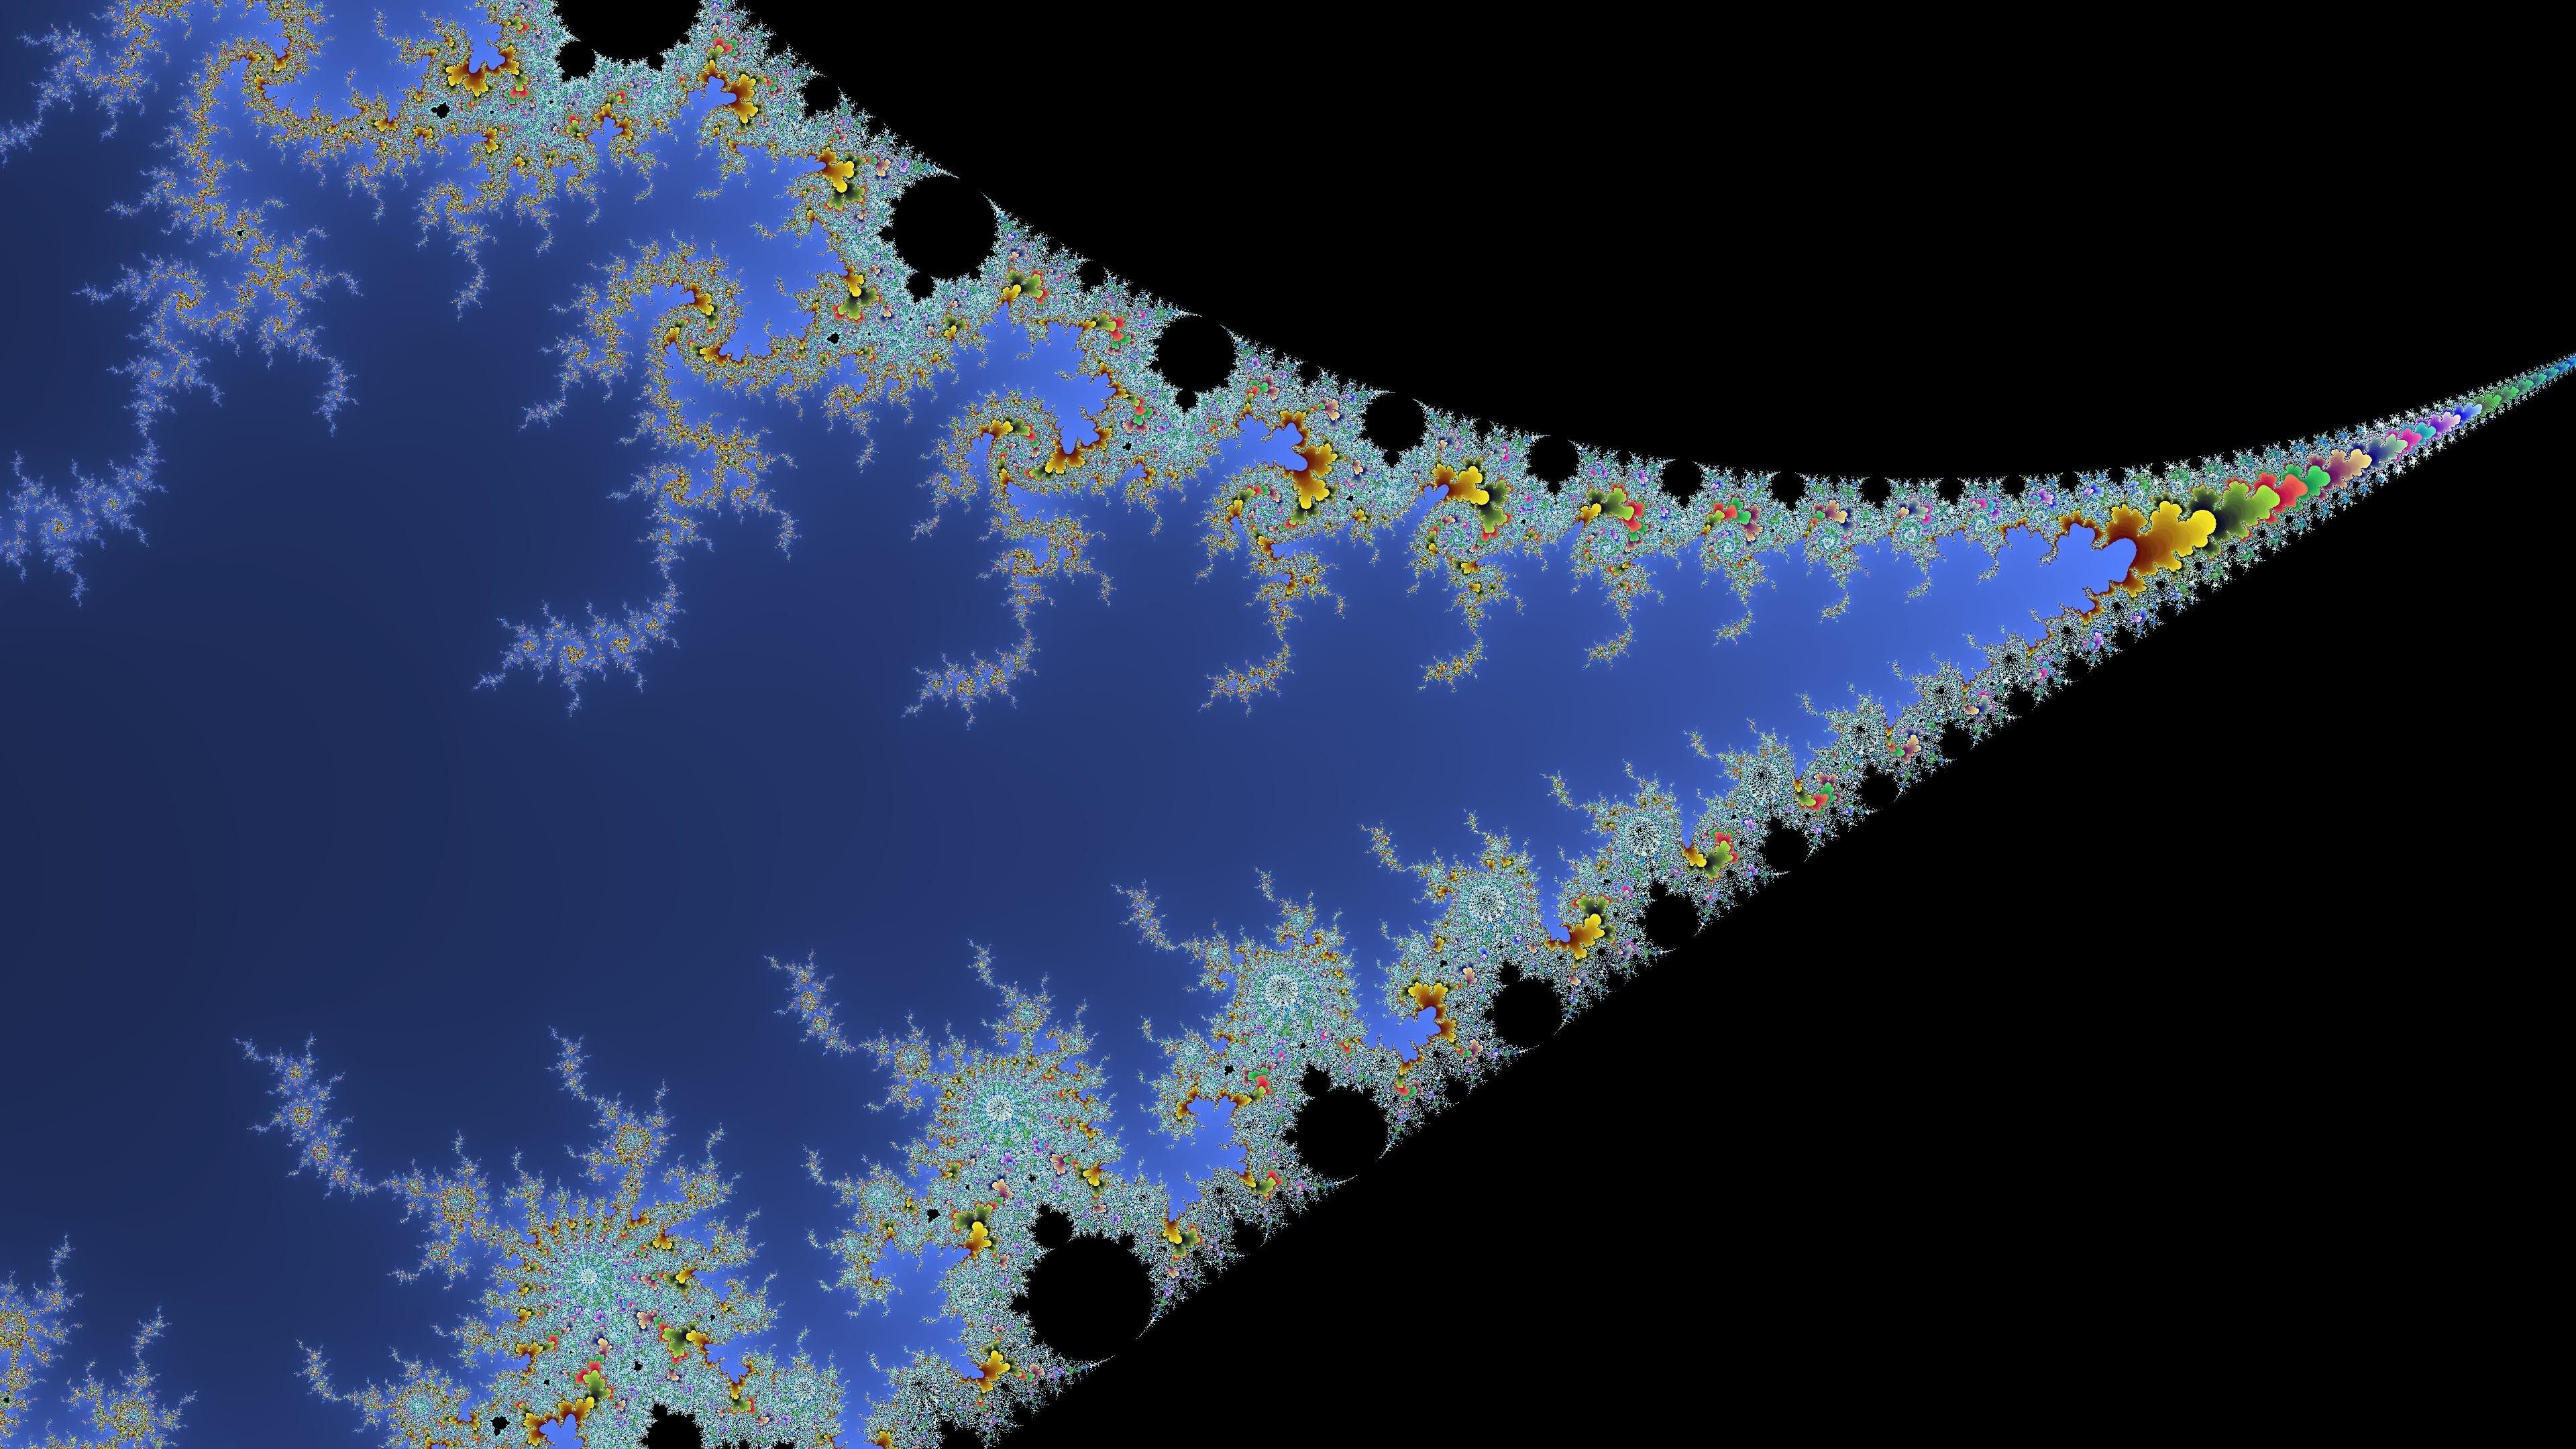
\includegraphics[scale = 0.4, angle = 270, origin = c]{AnalisiComplessaCover}};
\end{titlepage}
\nopagecolor
\tableofcontents

\chapter{Nozioni Introduttive}
\section{Funzioni Olomorfe}
\begin{boxdef}{Funzione Olomorfa}
\begin{mydef}
Data la funzione $f:\Omega\longrightarrow \C$, definita sull'insieme $\Omega\subseteq \C$, e dato il punto $w\in \Omega^\circ$, $f$ si dice olomorfa in $w$ se esiste il seguente limite:
$$
\lim_{h\to 0} \frac{f(w+h)-f(w)}{h}.
$$
In tal caso, chiamiamo tale limite derivata di $f$ in $w$, e lo indichiamo con $f'(w)$.
\end{mydef}
\end{boxdef}
\begin{mynota}
Alle volte il termine olomorfa viene sostituito dalle espressioni "differenziabile in senso complesso" oppure "regolare".
\end{mynota}
È scontato notare la simiglianza tra la definizione appena data e la differenziabilità di funzioni reali di una variabile, ed infatti notiamo due cose:
\begin{myobs}
Se $f:\Omega \longrightarrow \C$, è olomorfa in $w\in \Omega^\circ$, allora $f$ è continua in $w$.\\
Questo perché possiamo scrivere:
$$
|f(w+h)-f(w)| = |h| \left|\frac{f(w+h)-f(w)}{h}\right|,
$$
e dunque $\lim_{h \to 0} |f(w+h)-f(w)| = \lim_{h \to 0} |h||f'(w)| = 0$.
\end{myobs}
\begin{myobs}
Un'altra analogia con il caso reale è il seguente fatto. Data $f:\Omega \longrightarrow \C$, ed $w\in \Omega^\circ$ si ha che $f$ è olomorfa in $w$ se e solo se esiste un numero complesso $\alpha\in \C$, ed una funzione $\varepsilon:\Ball{r}{0}\longrightarrow \C$ con $\varepsilon(h)/h \to 0$ per $h \to 0$, tale che per ogni $h\in \Disc{r}{0}$ valga 
\begin{equation}\label{eq:FunzioneOlomorfaOPiccolo}
f(w+h)-f(w) = \alpha h + \varepsilon(h).
\end{equation}
Se $f$ è olomorfa in $w$, allora scrivendo:
$$
f(w+h)-f(w) = \frac{h}{h}(f(w+h)-f(w)) = h \frac{f(w+h)-f(w)}{h},
$$
poiché il rapporto a incrementale tende a $f'(w)$ per $h \to 0$, abbiamo che esiste una funzione $\tau$ (definita in un intorno di $0$) per cui $\tau(h) \to 0$ per $h \to 0$, e per cui il rapporto incrementale è uguale a $f'(w) + \tau(h)$. A questo punto abbiamo:
$$
f(w+h)-f(w) = h(f'(w)+\tau(h)) = h \cdot f'(w) + h\tau(h),
$$
e dunque basta chiamare $\alpha = f'(w)$, e $\varepsilon(h) := h\tau(h)$.\\
Viceversa calcolando il limite del rapporto incrementale abbiamo:
$$
\lim_{h \to 0} \frac{f(w+h)-f(w)}{h} = \lim_{h \to 0} \alpha + \frac{\varepsilon(h)}{h} = \alpha,
$$
e quindi $f$ è olomorfa in $w$, e $f'(w) = \alpha$. 
\end{myobs}
Fissiamo della notazione: dato $\alpha \in \C$, definiamo $\Lambda_\alpha:\C\ni z \longmapsto \alpha z \in \C$. Nota che questa mappa è $\C$-lineare, e che permette di riscrivere (\ref{eq:FunzioneOlomorfaOPiccolo}) nel seguente modo:
$$
f(w+h)-f(w) = \Lambda_\alpha(h) + \varepsilon(h).
$$
Capiremo più avanti come il fatto che questa mappa sia $\C$-lineare darà all'olomorfia proprietà molto distinte dalla differenziabilità in senso reale.
\begin{myes}
La funzione $f:\C \ni z \longmapsto z\in \C$ è olomorfa, e vale $f'(z) = 1$ per ogni $z\in \C$, dal momento che:
$$
\lim_{h \to 0} \frac{f(z+h)-f(z)}{h} = \lim_{h \to 0} \frac{z+h-z}{h} = \lim_{h \to 0}\frac{h}{h} = \lim_{h \to 0} 1 = 1.
$$
In modo altrettanto non sorprendente, ogni funzione costante è olomorfa, con derivata identicamente nulla.
\end{myes}
\begin{myes}\label{es:FunzioneDiConiugioNonOlomorfa}
La funzione $f: \C \ni z \longmapsto \barra{z}\in \C$ non è olomorfa in alcun punto, siccome per ogni $z\in \C$ si ha per ogni $h\in \C$:
$$
\frac{f(z+h)-f(z)}{h} = \frac{\barra{z+h}-\barra{z}}{h} = \frac{\barra{z}+\barra{h}-\barra{z}}{h} = \frac{\barra{h}}{h},
$$
che non ammette limite per $h \to 0$, siccome prendendo $h$ reale tale limite sarebbe 0, mentre prendendo $h$ immaginario, esse sarebbe $-1$.\\
Questo esempio fa luce su un fatto che uno potrebbe prendere per vero. Questa mappa può essere identificata con la funzione $\R^2\ni (x,y) \longmapsto (x,-y)\in \R^2$, dove $(x,y)\longmapsto x$ è la parte reale di $f$, e $(x,y)\longmapsto -y$ è la parte immaginaria di $f$. La mappa in questione è $\mathscr{C}^\infty$, eppure la funzione $f$ non è olomorfa.\\
Dunque l'olomorfia di una funzione $f$ non è legata alla regolarità di $\Re(f)$ e $\Im(f)$.
\end{myes}
Grazie a (\ref{eq:FunzioneOlomorfaOPiccolo}), si riescono a dimostrare tutti i risultati principali sull'algebra delle derivate. Omettiamo le dimostrazioni dal momento che seguono per filo e per segno il caso reale.
\begin{boxpro}
\begin{mypropo}\label{pro:AlgebraDerivate}
Siano $f,g:\Omega \longrightarrow \C$ due funzioni olomorfe in $w\in \Omega^\circ$. Allora:
\begin{itemize}
\item[$(i)$] $f+g$ è olomorfa in $w$, e vale $(f+g)'(w) = f'(w)+g'(w)$.
\item[$(ii)$] Per ogni $\alpha\in \C$ si ha che $\alpha f$ è olomorfa in $w$, e vale $(\alpha f)'(w) = \alpha f'(w)$.
\item[$(iii)$] $fg$ è olomorfa in $w$, e vale $(fg)'(w) = f'(w)g(w)+g'(w)f(w)$.
\item[$(iv)$] se $g(w) \neq 0$, allora $f/g$ è olomorfa in $w$, e vale:
$$
\left(\frac{f}{g}\right)'(w) = \frac{f'(w)g(w)-g'(w)f(w)}{[g(w)]^2}
$$
\end{itemize} 
\end{mypropo}
\end{boxpro}
\begin{myes}
Con quanto sappiamo ora possiamo calcolare alcune derivate elementari. La funzione $f:\C\ni z \longmapsto z^2\in \C$, usando la regola di Leibniz, ha derivata $f'(z) = z \cdot 1 + z \cdot 1$, e, ragionando per induzione, si dimostra che la funzione $g:\C \ni z \longmapsto z^n\in \C$ (con $n \geq 0$) è olomorfa e ha derivata $g'(z) = n z^{n-1}$.\\
In realtà tale uguaglianza vale per ogni intero, e questo si dimostra usando la regola del quoziente per $z \longmapsto 1/z$, il resto si fa per induzione sempre usando la regola del quoziente.\\
Usando le altre regole, si riesce a dimostrare che ogni funzione polinomiale e razionale è olomorfa (le ultime solo nei punti in cui il denominatore non si annulla). 
\end{myes}
Anche per la regola della catena si ha un risultato analogo al caso reale, e, come prima, la dimostrazione è identica.
\begin{boxpro}
\begin{mypropo}\label{pro:RegolaCatena}
Siano $\Omega,\Lambda\subseteq \C$, $w\in \Omega^\circ$, $f:\Omega\longrightarrow \C$ con immagine contenuta in $\Lambda$ e $f(w)\in \Lambda^\circ$, e sia $g: \Lambda \longrightarrow \C$. Allora se $f$ è olomorfa in $w$, e $g$ è olomorfa in $f(w)$, risulta che $g\circ f: \Omega \longrightarrow \C$ è olomorfa in $w$, e vale:
$$
(g\circ f)'(w) = g'(f(w))f'(w).
$$
\end{mypropo}
\end{boxpro}
\begin{myes}\label{es:Esercizio04/10}
Consideriamo la funzione $f:\C \ni x+\i y\longmapsto |x||y|\in \C$. Dimostriamo che $f$ è olomorfa in $0$ e da nessun'altra parte.
Per quanto riguarda $0$, abbiamo che per ogni $h = h_1+\i h_2\in \C$ risulta:
$$
\left|\frac{f(0+h)-f(0)}{h}\right| = \frac{|h_1||h_2|}{\sqrt{h_1^2+h_2^2}} \leq \frac{h_1^2+h_2^2}{\sqrt{h_1^2+h_2^2}} = \sqrt{h_1^2+h_2^2},
$$
perciò:
$$
\lim_{h \to 0} \left|\frac{f(0+h)-f(0)}{h}\right| = \lim_{(h_1,h_2)\to (0,0)} \sqrt{h_1^2+h_2^2} = 0,
$$
che prova che il limite del rapporto incrementale è $0$. 
Sia ora $w = a+\i b \neq 0$, ossia con $a$ e $b$ non entrambi nulli. Abbiamo che, per ogni $h = h_1+\i h_2$:
\begin{equation}\label{eq:Equazione1Esercizio04/10}
\frac{f(w+h)-f(w)}{h} = \frac{|a+h_1||b+h_2|-|a||b|}{h_1+\i h_2},
\end{equation}
quindi se $f$ fosse olomorfa in $w$, avremmo come limite per $h \to 0$ $f'(w)$ anche restringendoci ad $h$ reale, però nota che:
$$
\lim_{h \to 0} \frac{f(w+h)-f(w)}{h} = \lim_{h_1 \to 0} |b| \frac{|a+h_1|}{|h_1|},
$$
non esiste se $b \neq 0$, mentre è uguale a $0$ se $b = 0$. Quindi abbiamo dimostrato che $f$ non è olomorfa in $a+\i b$ se $b \neq 0$. Supponiamo quindi $b = 0$. Riprendendo (\ref{eq:Equazione1Esercizio04/10}), se $f$ fosse olomorfa in $w$, restringendoci ad $h$ immaginario avremmo:
$$
\lim_{h \to 0} \frac{f(w+h)-f(w)}{h} = \lim_{h_2 \to 0} |a|\frac{|h_2|}{\i h_2}
$$
che è un limite che non esiste ($a \neq 0$).
\end{myes}
In questo corso non studieremo le funzioni di questo tipo, ossia quelle olomorfe in punti isolati, ma ci concentreremo sulle funzioni che sono olomorfe su tutto un aperto.\\
Dato un aperto $\Omega\subseteq \C$, indichiamo con $H(\Omega)$ l'insieme delle funzioni definite su $\Omega$ tale che sono olomorfe in ogni suo punto.\\
Le proprietà in (\ref{pro:AlgebraDerivate}) ci permettono di dire che $H(\Omega)$ è uno spazio vettoriale complesso (sarebbe anche un Algebra con il prodotto puntuale di funzioni, ma non ci interessa più di tanto quest'ultimo aspetto).
\section{Serie di potenze}
In questa sezione andiamo a indagare un particolare tipo di funzioni, le serie di potenze, già viste nel caso reale.
Le serie di potenze in campo complesso non sono troppo dissimili dalle serie complesse in senso reale, se non per un paio di aspetti che riguardano solo le dimostrazioni.\\
\indent
Prima di cominciare l'esposizione sulle serie di potenze, ricordiamo un ricordato generale sulle serie di funzioni che vale anche in ambito complesso.
\begin{boxteo}{Criterio di Weierstrass}
\begin{myteo}
Sia $\sum_n f_n$ una serie di funzioni definite in $\Omega\subseteq \C$ per cui esiste una serie $\sum_n c_n$ a termini positivi convergente tale che $|f_n(z)| \leq c_n$ per ogni indice $n$ e $z\in \Omega$. Allora la serie di funzioni $\sum_{n} f_n$ converge uniformemente su $\Omega$.
\end{myteo}
\end{boxteo}
\noindent
Nota che dire che $|f_n(z)| \leq c_n$ per ogni indice $n$ e $z\in \Omega$ equivale a dire che $\sup_{z\in \Omega} |f_n(z)| \leq c_n$ per ogni indice $n$; in alternativa quindi le ipotesi del teorema sopra sono equivalenti a dire che $\sum_n f_n$ è una serie di funzioni per cui $\sum_n \sup_{z\in \Omega} |f_n(z)|$ converge.\\
\indent
Chiameremo serie di potenze una qualsiasi serie di funzioni $\sum_n f_n$, dove $f_n:\C\longrightarrow \C$ è del tipo $f_n(z) = a_n (z-z_0)^n$, con $\{a_n\}_{n = 0}^\infty\subseteq \C$ e $z_0\in \C$ è fissato. Come per il caso reale, per lo sviluppo della teoria ci si può solo preoccupare del caso in cui $z_0 = 0$, in quanto per ricondursi a tale caso basta considerare $g_n: \C \ni z \longmapsto f_n(z+z_0)\in \C$.
Data la serie di potenze $\sum_n a_n z^n$, chiamiamo raggio di convergenza il seguente numero reale (esteso):
$$
R = \frac{1}{\displaystyle\limsup_{n\to\infty} \sqrt[n]{|a_n|}},
$$
intendendo $R = 0$ quando il limite superiore è $+\infty$, ed $R = +\infty$ quando esso è uguale a $0$.
\begin{boxteo}{Teorema di Hadamard}
\begin{myteo}
Sia $\sum_n a_n z^n$ una serie di potenze in campo complesso con raggio di convergenza $R$. Allora valgono le seguenti:
\begin{itemize}
\item[$(i)$] Se $R = 0$, la serie di potenze in questione converge solo per $ z = 0$.
\item[$(ii)$] Se $0 < R < +\infty$, la serie converge assolutamente su $\Disc{R}{0}$ e diverge sull'insieme $\C\tolto\barra{\Disc{R}{0}} = \{z\in \C:\ |z| > R\}$. Inoltre la serie converge uniformemente sui compatti $K$ del disco $\Disc{R}{0}$ $($ossia i compatti di $\C$ contenuti nel disco $\Disc{R}{0})$.
\item[$(iii)$] Se $ R = +\infty$, allora la serie converge assolutamente su tutto $\C$ e converge uniformemente sui compatti $K \subseteq \C$.
\end{itemize}
\end{myteo}
\tcblower
\begin{proof}
Dimostriamo solo il punto $(ii)$. Sia $z\in \Disc{R}{0}$, e prendi $\rho$ con $|z| < \rho < R$. Si ha dalla definizione di raggio di convergenza che:
$$
\limsup_{n \to\infty} |a_nR^n|^{1/n} = 1,
$$
dunque dato $\varepsilon > 0$, il numero $1+\varepsilon$ è un maggiorante definitivo di $\{|a_nR^n|^{1/n}\}$, ossia che esiste un $\barra{n}$ tale che per ogni $n\geq \barra{n}$, $|a_nR^n|^{1/n} < 1+\varepsilon$, ossia $|a_nR^n| < (1+\varepsilon)^n$, perciò per $n\geq \barra{n}$ si ha:
$$
|a_n z^n| = |a_n| |z|^n \leq \frac{(1+\varepsilon)^n}{R^n}|z|^n \leq \left(\frac{1+\varepsilon}{R}\right)^n\rho^n = \left((1+\varepsilon)\frac{\rho}{R}\right)^n,
$$
dunque scegliendo $\varepsilon > 0$ con $(1+\varepsilon) \rho/R < 1$, ossia $\varepsilon < R/\rho - 1$, si ottiene per criterio del confronto che la serie numerica $\sum_n a_n z^n$ converge assolutamente. Con ciò si dimostra la convergenza puntuale in $\Disc{R}{0}$. Ora supponiamo che $z\in \C\tolto \barra{\Disc{R}{0}}$, ossia $|z| > R$. Poiché $\limsup_{n\to\infty} |a_n|^{1/n} = 1/R$, esiste una sottosuccessione $\{a_{n_k}\}_{k = 1}^\infty$ con $|a_{n_k}|^{1/n_k}$ tendente ad $1/R$ per $k \to \infty$, perciò si ha $|a_{n_k} z^{n_k}|^{1/n_k}| > |a_{n_k} R^{n_k}|^{1/n_k} = |a_{n_k}|^{1/n_k}$, che tende ad $1$ per $k \to \infty$, ma quindi non può accadere che $a_n z^n \to 0$ per $n\to\infty$, che impedisce la convergenza di $\sum_{n} a_n z^n$.\\
Infine sia $K \subseteq \Disc{R}{0}$ un compatto. Siccome la mappa $z \longmapsto |z|$ è continua essa ammetterà massimo, diciamo $M$, su $K$, e quindi essendo $M$ minore o uguale del massimo che questa funzione ammette su $\barra{\Disc{R}{0}}\supseteq K$, si avrà $M < R$. Quindi per ogni $z\in K$ si ha $|a_n z^n| \leq |a_n M^n|$, che è il termine generale di una serie convergente, perciò applicando il criterio di Weierstrass otteniamo la convergenza uniforme.
\end{proof}
\end{boxteo}
\begin{myobs}
Si può dimostrare senza troppa difficoltà che se $\{a_n\}_{n = 1}^\infty\subseteq \C$ è una successione di numeri complessi non definitamente nulla, allora:
$$
\liminf_{n\to\infty} \left|\frac{a_{n+1}}{a_n}\right|\leq \liminf_{n\to\infty} |a_n|^{1/n}\leq \limsup_{n\to\infty} |a_n|^{1/n} \leq \limsup_{n\to\infty} \left|\frac{a_{n+1}}{a_n}\right|,
$$
dunque se:
$$
\lim_{n \to \infty} \left|\frac{a_{n+1}}{a_n}\right| = \ell\in [0,+\infty],
$$
risulta che $\ell$ è il raggio di convergenza della serie di potenze $\sum_n a_nz^{n}$. Con questo si può calcolare più facilmente il raggio di convergenza di certe serie, ad esempio:
$$
\sum_{n = 0}^\infty \frac{z^n}{n!}
$$
ha raggio di convergenza $+\infty$ siccome:
$$
\lim_{n \to\infty} \frac{n!}{(n+1)!} = \lim_{n\to\infty} \frac{1}{n+1} = 0.
$$
\end{myobs}
Ora indaghiamo che tipo di relazioni sussistano tra le serie di potenze e l'olomorfia di funzioni, in particolare ci chiediamo quando una serie di potenze è olomorfa e dove.\textcolor{red}{qui potresti migliorare}
\begin{boxteo}{}
\begin{myteo}
Sia $\sum_n a_n z^n$ una serie di potenze con raggio di convergenza $R$ positivo, e sia $f: \Disc{R}{0} \ni z \longmapsto \sum_{n = 0}^\infty a_n z^n \in \C$. Allora $f$ è olomorfa e la sua derivata complessa è data da:
$$
f'(z) = \sum_{n = 1}^\infty n a_n z^{n-1}
$$
per ogni $z\in \Disc{R}{0}$.
\end{myteo}
\tcblower
\begin{proof}
In primo luogo notiamo che la serie $\sum_n n a_n z^{n-1}$ ha lo stesso raggio di convergenza della serie originale che definisce $f$, e questo è dovuto al fatto che $\lim_{n \to \infty} |n|^{1/n} = 1$, che permette di dire che $\limsup_{n \to \infty} |na_n|^{1/n} = \limsup_{n\to\infty} |a_n|^{1/n}$. Definiamo ora la funzione $g:\Disc{R}{0}\ni z \longmapsto \sum_{n = 1}^\infty n a_n z^{n-1}\in \C$. Vogliamo mostrare che per ogni $z_0\in \C$ vale $f'(z_0) = g(z_0)$, ossia:
$$
\lim_{h \to 0} \frac{f(z_0+h)-f(z_0)}{h} = g(z_0).
$$
Il modo in cui mostreremo questo limite è mediante la definizione. Sia dunque $\varepsilon>0$; vogliamo trovare un $\delta > 0$ per la quale per ogni $h\in \Disc{\delta}{0}$ risulti:
$$
\left|\frac{f(z_0+h)-f(z_0)}{h}-g(z_0)\right|< \varepsilon.
$$
L'idea è quella di stimare questo modulo. Prima però prendiamo $r > 0$ con $|z_0| < r < R$, e scriviamo per ogni indice $N$, e per ogni $z\in \Disc{R}{0}$:
$$
f(z) = \underbrace{\sum_{n = 0}^N a_n z^n}_{S_N(z)} + \underbrace{\sum_{n = N+1}^{\infty} a_n z^n}_{E_N(z)}.
$$
Per ogni $h\in \Disc{r-|z_0|}{0}$ avremo:
\begin{multline*}
\frac{f(z_0+h)-f(z_0)}{h}-g(z_0) =\\
= \frac{S_N(z_0+h)-S_N(z_0)}{h}-S_N'(z_0) + S_N'(z_0)-g(z_0) + \frac{E_N(z_0+h)-E_N(z_0)}{h}
\end{multline*}
da cui si ottiene:
\begin{multline}\label{eq:teo:TeoremaDerivataSerieDiPotenze}
\left|\frac{f(z_0+h)-f(z_0)}{h}-g(z_0)\right|\leq\\
\leq\left|\frac{S_N(z_0+h)-S_N(z_0)}{h}-S_N'(z_0)\right| + |S_N'(z_0)-g(z_0)| + \left|\frac{E_N(z_0+h)-E_N(z_0)}{h}\right|.
\end{multline}
Per quanto riguarda il termine al centro, avendo $\lim_{N \to \infty} S_N'(z_0) = g(z_0)$, esisterà un $N_1$ per cui per $N \geq N_1$ risulta $|S_N'(z_0)-g(z_0)| < \varepsilon/3$. Concentriamo la nostra attenzione sull'ultimo termine. Notiamo che:
$$
\frac{E_N(z_0+h)-E_N(z_0)}{h} = \sum_{n = N+1}^{\infty} a_n \frac{(z_0+h)^n-z_0^n}{h},
$$
quindi:
$$
\left|\frac{E_N(z_0+h)-E_N(z_0)}{h}\right| \leq \sum_{n = N+1}^{\infty} |a_n| \left|\frac{(z_0+h)^n-z_0^n}{h}\right|,
$$
ma applicando la formula per la differenza di potenze $n$-esime otteniamo:
$$
(z_0+h)^n-z_0^n = (z_0+h-z_0)\big((z_0+h)^{n-1}+(z_0+h)^{n-2}z_0+\cdots+z_0^{n-1}\big),
$$
e da qui, essendo $|z_0| < r$ e $|z_0+h|\leq |z_0|+|h| < |z_0| + r-|z_0| = r$, si vede che:
$$
\left|\frac{(z_0+h)^n-z_0^n}{h}\right| \leq nr^{n-1},
$$
e quindi arriviamo a dire che:
$$
\left|\frac{E_N(z_0+h)-E_N(z_0)}{h}\right| \leq \sum_{n = N+1}^\infty |a_n| n r^{n-1},
$$
ma siccome $r < R$, abbiamo che la serie sopra converge, e portando $N \to \infty$ si vede che il lato destro tende a $0$, permettendoci di dire che:
$$
\lim_{N \to\infty} \left|\frac{E_N(z_0+h)-E_N(z_0)}{h}\right| = 0,
$$
dunque esisterà un $N_2$ per cui per ogni $N \geq N_2$ risulterà che il termine sopra è minore di $\varepsilon/3$.\\
Infine, occupiamoci del primo termine in (\ref{eq:teo:TeoremaDerivataSerieDiPotenze}); questo è quello più facile in quanto per definizione di derivata complessa tale modulo può essere reso arbitrariamente piccolo, in particolare per ogni $N$ esisterà un $\delta_N>0$ per cui per ogni $h\in \Disc{\delta}{0}$ risulterà che tale modulo è minore di $\varepsilon/3$. A questo punto prendendo $N \geq \max\{N_1,N_2\}$ e $\delta = \min\{\delta_N,r-|z_0|\}$, avremo che per ogni $h\in \Disc{\delta}{0}$, ciascun termine a secondo membro di (\ref{eq:teo:TeoremaDerivataSerieDiPotenze}) è inferiore di $\varepsilon/3$, che era ciò che volevamo dimostrare.
\end{proof}
\end{boxteo}
\noindent
Ora ci poniamo come obiettivo quello di estendere le funzioni elementari che conosciamo in campo reale al campo complesso. Usando le serie di potenze, espanderemo la funzione esponenziale, il seno, il coseno, e via dicendo.\\
Definiamo prima la funzione più importante.
\begin{boxdef}{La funzione esponenziale}
\begin{mydef}
Definiamo la funzione esponenziale $\exp:\C\longrightarrow \C$ ponendo:
$$
\exp(z) = \sum_{k = 0}^\infty \frac{z^k}{k!}.
$$
\end{mydef}
\end{boxdef}
\noindent
Abbiamo già osservato che la serie di potenze che definisce $\exp$ ha raggio di convergenza $+\infty$, e quindi la definizione appena data è ben posta.
\begin{myobs}
Osserviamo prima le proprietà più immediate:
\begin{itemize}
\item $$
	  \exp(0) = \sum_{k = 0}^\infty \frac{0^k}{k!} = 0^0 = 1.
      $$
\item $$
	  \exp(1) = \sum_{n = 0}^\infty \frac{1}{n!} = \e
	  $$.
\item $\exp(\barra{z}) = \barra{\exp(z)}$, questo perché:
$$
\exp(\barra{z}) = \sum_{n = 0}^\infty \frac{(\barra{z})^n}{n!} = \sum_{n = 0}^\infty \frac{\barra{(z^n)}}{n!} = \barra{\left(\displaystyle{\sum_{n = 0}^\infty \frac{z^n}{n!}}\right)} = \barra{\exp(z)}.
$$
(l'ultimo passaggio è giustificato dalla continuità della funzione $z \longmapsto \barra{z}$).
\item $\exp'(z) = \exp(z)$, siccome:
$$
\left(\sum_{n = 0}^\infty \frac{z^n}{n!}\right)' =              
\sum_{n = 1}^\infty \frac{nz^{n-1}}{n!} = \sum_{n = 1}^
\infty \frac{z^{n-1}}{(n-1)!} = \sum_{k = 0}^\infty \frac{z^k}{k!} = \exp(z).
$$
\item Per ogni $x\in \R$, si ha $\exp(x) = \e^x$.\\
Considera la funzione $y:\R \longrightarrow \R$ data da $y(x) = \exp(x)$. Nota che per ogni $x \in \R$ il limite del rapporto incrementale di $y(x)$ ed è uguale al limite complesso del rapporto incrementale di $\exp(x)$, dunque $y'(x) = \exp'(x) = y(x)$. Notando che $y(0) = \exp(0) = 1$, abbiamo che $y$ soddisfa il seguente problema di cauchy:
$$
\begin{cases}
y'(x) = y(x)\\
y(0) = 1
\end{cases}
$$
e dunque, siccome l'unica soluzione di tale problema di cauchy è la funzione $x \longmapsto \e^x$, deve essere che $y(x) =\e^x$ per ogni $x\in \R$.
\end{itemize}
\end{myobs}
La prossima proprietà che andremo a dimostrare sarà il fatto che la funzione esponenziale trasforma somma in prodotto, per farlo però abbiamo bisogno di giustificare un passaggio non esattamente ovvio.
\begin{boxteo}{}
\begin{myteo}
Siano $f(z) = \sum_{n = 0}^\infty a_n z^n$ e $g(z) = \sum_{n = 0}^\infty b_n z^n$ due serie assolutamente convergenti in $\Disc{R}{0}$. Allora la serie $\sum_n c_n z^n$, dove
$$
c_n = \sum_{k = 0}^n a_kb_{n-k},
$$
converge nel disco $\Disc{R}{0}$ e la sua somma, chiamata $h(z)$, soddisfa $h(z) = f(z)g(z)$ per ogni $z\in \Disc{R}{0}$.
\end{myteo}
\end{boxteo}

\begin{boxpro}
\begin{mypropo}
La funzione esponenziale è un omomorfismo dal gruppo additivo dei numeri complessi $(\C,+)$ al gruppo moltiplicativo $(\C^\times,\cdot)$.
\end{mypropo}
\tcblower
\begin{proof}
Dimostriamo prima che $\exp(z+w) = \exp(z)\exp(w)$ per ogni $z,w\in \C$; una volta dimostrato ciò, osservando che per ogni $z\in \C$ che:
$$
1 = \exp(0) = \exp(z-z) = \exp(z) \exp(-z),
$$
otterremo che $\exp(z)^{-1} = \exp(-z)$, di conseguenza deducendo che $\exp$ non assume mai il valore $0$. Siano quindi $z,w\in \C$. Per il teorema precedente risulta
\begin{align*}
\exp(z)\exp(w) &= \left(\sum_{n = 0}^\infty \frac{z^n}{n!}\right)\left(\sum_{m = 0}^\infty \frac{w^m}{m!}\right) = \sum_{n = 0}^\infty \left(\sum_{k = 0}^n \frac{z^k}{k!}\frac{w^{n-k}}{(n-k)!}\right)\\
&= \sum_{n = 0}^\infty \frac{1}{n!}\sum_{k = 0}^n \frac{n!}{k!(n-k)!}z^kw^{n-k} = \sum_{n = 0}^\infty \frac{(z+w)^n}{n!} = \exp(z+w).
\end{align*}
\end{proof}
\end{boxpro}
\noindent 
Questa proposizione ha una serie di conseguenze:
\begin{myobs}
Sia $x\in \R$. Allora si ha che:
$$
|\exp(\i x)|^2 = \exp(\i x)\barra{\exp(\i x)} = \exp(\i x)\exp(\barra{\i x}) = \exp(\i x)\exp(-\i x) = \exp(\i x-\i x) = \exp(0) =1.
$$
\end{myobs}
\begin{myobs}
Sia $z\in \C$ un numero complesso qualunque. Cerchiamo di determinare $\exp(\i z)$:
$$
\exp(\i z) = \sum_{n = 0}^\infty \frac{(\i z)^n}{n!} = \sum_{n = 0}^\infty \frac{\i^nz^n}{n!},
$$
se spezziamo la serie in termini pari e dispari (possiamo spezzare la serie senza problemi, abbiamo convergenza assoluta), otteniamo:
\begin{equation}\label{eq:MotivazioneSenoCosenoComplessi}
\sum_{k = 0}^\infty \frac{(-1)^k}{(2k)!}z^{2k} + \i \sum_{k = 0}^\infty \frac{(-1)^k}{(2k+1)!}z^{2k+1}.
\end{equation}
Queste due serie di potenze, in modo simile alla funzione esponenziale, convergono su tutto $\C$, e sono simili alle serie di Taylor centrate in $0$ del coseno e del seno rispettivamente.
\end{myobs}
È giunto il momento di estendere il seno e il coseno ai numeri complessi.
\begin{boxdef}{Seno e Coseno nel campo complesso}
\begin{mydef}
Definiamo il coseno complesso $\Cos:\C\longrightarrow \C$ ponendo per ogni $z\in \C$:
$$
\Cos(z) = \sum_{k = 0}^\infty \frac{(-1)^k}{(2k)!} z^{2k},
$$
e definiamo il seno complesso $\Sin:\C\longrightarrow \C$ ponendo per ogni $z\in \C$:
$$
\Sin(z) = \sum_{k = 0}^\infty \frac{(-1)^k}{(2k+1)!}z^{2k+1}.
$$
\end{mydef}
\end{boxdef}
\noindent
Con l'introduzione di queste due funzioni possiamo scrivere (\ref{eq:MotivazioneSenoCosenoComplessi}) in un modo più compatto:
\begin{equation}\label{eq:FormulaEuleroFormaGeneraleCosSin}
\exp(\i z) = \Cos(z)+\i\Sin(z).
\end{equation}
Per quanto visto prima, abbiamo che per ogni $x\in \R$, $\Cos(x) = \cos(x)$, e $\Sin(x) = \sin(x)$, e quindi per ogni $x \in \R$ si ha:
\begin{equation}\label{eq:FormulaEuleroRealiExp}
\exp(\i x) = \cos(x)+\i\sin(x).
\end{equation}
Da qui in poi faremo a meno di usare i simboli $\exp,\Cos,\Sin$ per l'esponenziale, il coseno, ed il seno, ed useremo le notazioni più familiari per ogni $z\in \C$: $\e^z = \exp(z)$, $\cos(z) = \Cos(z)$, e $\sin(z) = \Sin(z)$.\\
Ora avremo l'opportunità di vedere la prima divergenza dall'analisi reale in analisi complessa: la periodicità della funzione esponenziale.
\begin{myobs}
Una funzione $f:\C \longrightarrow \C$ si dice periodica se esiste un $w\in \C$ tale che per ogni $z\in \C$ risulta $f(z+w) = f(z)$, ed in tal caso diciamo che $f$ ha periodo $w$.\\
Nota che $\e^{2\pi \i} = \cos(2\pi) + \i \sin(2\pi) = 1$, dunque per ogni $z\in \C$:
$$
\e^{z+2\pi \i} = \e^z \e^{2\pi \i} = \e^z.
$$
\end{myobs}
\begin{myobs}
Sia $z\in \C$. Nota che:
$$
\cos(-z) = \sum_{k = 0}^\infty \frac{(-1)^k}{(2k)!}(-z)^{2k} = \sum_{k = 0}^\infty \frac{(-1)^k}{(2k)!}(-1)^{2k}z^{2k} = \sum_{k = 0}^\infty \frac{(-1)^k}{(2k)!}z^{2k} = \cos(z),
$$
dunque il coseno complesso, come la sua controparte reale, è una funzione pari. Analogamente:
\begin{align*}
\sin(-z) &= \sum_{k = 0}^\infty \frac{(-1)^k}{(2k+1)!}(-z)^{2k+1} = \sum_{k = 0}^\infty \frac{(-1)^k}{(2k+1)!}(-1)^{2k+1}z^{2k+1} = \sum_{k = 0}^\infty \frac{(-1)^k}{(2k+1)!}(-1)z^{2k+1} \\
&= - \sum_{k = 0}^\infty \frac{(-1)^k}{(2k+1)!}z^{2k+1} = -\sin(z).
\end{align*}
\end{myobs}
\begin{myobs}
Sia $z\in \C$. Dalla formula di Eulero (\ref{eq:FormulaEuleroFormaGeneraleCosSin}) abbiamo che $\e^{\i z} = \cos(z) + \i\sin(z)$. Prendendo $-z$ al posto di $z$, da quanto visto nell'osservazione precedente risulterà che $\e^{-\i z} = \cos(-z) + \i\sin(-z) = \cos(z)-\i\sin(z)$, e dunque:
$$
\begin{cases}
\e^{\i z} = \cos(z) + \i\sin(z)\\
\e^{-\i z} = \cos(z)-\i\sin(z) 
\end{cases} \implies \ \cos(z) = \frac{\e^{\i z}+\e^{-\i z}}{2},\quad \textup{ e }\quad \sin(z) = \frac{\e^{\i z}-\e^{-\i z}}{2\i}.
$$
Da queste due equazioni deduciamo che seno e coseno sono funzioni periodiche con periodo $2\pi$:
$$
\cos(z+2\pi) = \frac{\e^{\i(z+2\pi)}+\e^{-\i(z+2\pi)}}{2} = \frac{\e^{\i z+2\pi \i}+\e^{-\i z-2\pi \i}}{2} = \frac{\e^{\i z}+\e^{-\i z}}{2} = \cos(z),
$$
$$
\sin(z+2\pi) = \frac{\e^{\i(z+2\pi)}-\e^{-\i(z+2\pi)}}{2} = \frac{\e^{\i z+2\pi \i}-\e^{-\i z-2\pi \i}}{2\i} = \frac{\e^{\i z}-\e^{-\i z}}{2\i} = \sin(z).
$$
Questo potrebbe erroneamente sembrare una conseguenza della periodicità del seno e coseno reali, ma in realtà non c'è alcun legame, se una funzione da $\C$ in $\C$ è periodica se ristretta ai reali non c'è alcun motivo affinché essa sia periodica su tutto il piano complesso.
\end{myobs}
\begin{myobs}
Per ogni $z,w\in \C$ si ha:
$$
\cos(z+w) = \cos(z)\cos(w)-\sin(z)\sin(w)\quad \textup{ e }\quad\sin(z+w) = \sin(z)\cos(w)+\cos(w)\sin(z).
$$
Dimostriamo solo la prima, la seconda si dimostra in modo analogo.
\begin{gather*}
\cos(z)\cos(w)-\sin(z)\sin(w) = \left(\frac{\e^{\i z}+\e^{-\i z}}{2}\right)\left(\frac{\e^{\i w}+\e^{-\i w}}{2}\right) - \left(\frac{\e^{\i z}-\e^{-\i z}}{2\i}\right)\left(\frac{\e^{\i w}-\e^{-\i w}}{2\i}\right)\\
= \frac{1}{4}\left(\e^{\i z}\e^{\i w}+\e^{-\i z}\e^{\i w}+\e^{\i z}\e^{-\i w}+\e^{-\i z}\e^{-\i z}\right)+\frac{1}{4}\left(\e^{\i z}\e^{\i w}-\e^{-\i z}\e^{\i w}-\e^{\i z}\e^{-\i w}+\e^{-\i z}\e^{-\i w}\right)\\
= 2 \cdot \frac{1}{4}\left(\e^{\i z}\e^{\i w}+\e^{-\i z}\e^{-\i w}\right) = \frac{\e^{\i(z+w)}+\e^{-\i(z+w)}}{2} = \cos(z+w).
\end{gather*}
Siccome dalle formule di somma di angoli si deducono tutte le formule trigonometriche note, con questo dimostriamo la validità di quelle formule anche per i numeri complessi.
\end{myobs}
Passiamo ora alle funzioni iperboliche
\begin{boxdef}{Seno iperbolico e Coseno iperbolico}
\begin{mydef}
Definiamo il coseno iperbolico $\cosh:\C\longrightarrow \C$ ponendo per ogni $z\in \C$:
$$
\cosh(z) = \frac{\e^z+\e^{-z}}{2},
$$
e definiamo il seno iperbolico $\sinh:\C\longrightarrow \C$ ponendo per ogni $z\in \C$:
$$
\sinh(z) = \frac{\e^{z}-\e^{-z}}{2}.
$$
\end{mydef}
\end{boxdef}
\noindent
Le definizioni appena date per il seno e il coseno iperbolico coincidono con quelle date sui reali, quindi, per $z$ reale non ci sono ambiguità per quanto riguarda $\cosh(z)$ e $\sinh(z)$.\\
Come accadeva per seno e coseno, per ogni $z\in \C$ si ha $\sinh(-z) =-\sinh(z)$ e $\cosh(-z) = \cosh(z)$.
\begin{myobs}
Per i numeri complessi è facile vedere il legame che c'è tra le funzioni trigonometriche e quelle iperboliche, infatti per ogni $z\in \C$:
$$
\cos(z) = \frac{\e^{\i z}+\e^{-\i z}}{2} = \cosh(\i z),
$$
e
$$
\sin(z) = \frac{\e^{\i z}-\e^{-\i z}}{2\i} = \frac{1}{\i}\sinh(\i z) = -\i\sinh(\i z).
$$
D'altra parte abbiamo:
$$
\cos(\i z) = \frac{\e^{z}+\e^{-z}}{2} = \cosh(z),
$$
e
$$
\sin(\i z) = \frac{\e^{-z}-\e^{z}}{2\i} = -\frac{1}{\i}\sinh(z) = \i\sinh(z).
$$
Queste relazioni non sono da prendere sottogamba, ci permettono infatti di vedere delle proprietà del seno e del coseno drasticamente differenti dalle loro controparti reali.\\
Prendendo $x\in \R$ si ha $\cos(ix) = \cosh(x)$, ma il coseno iperbolico sui reali è illimitato, quindi il coseno complesso non è una funzione limitata. Analogamente per il seno si ha che $\sin(\i x) = \i\sinh(x)$, ed essendo il seno iperbolico sui reali illimitato, abbiamo che anche il seno complesso non è limitato.\\
Da queste relazioni possiamo scoprire una cosa ulteriore: dato il numero complesso $z$ di parte reale $x$ e parte immaginaria $y$, si ha che
$$
\sin(z) = \sin(x+\i y) = \sin(x)\cos(\i y)+\cos(x)\sin(\i y) = \sin(x)\cosh(y) + \i\cos(x)\sinh(y),
$$
e per quanto riguarda il coseno:
$$
\cos(z) = \cos(x+\i y) = \cos(x)\cos(\i y)-\sin(x)\sin(\i y) = \cos(x)\cosh(y)-\i\sin(x)\sinh(y).
$$
\end{myobs}
\begin{myobs}
Continuano a valere anche in campo complesso le seguenti formule
$$
\sinh(z+w) = \sinh(z)\cosh(w)+\cosh(z)\sinh(w)\quad \textup{ e }\quad \cosh(z+w) = \cosh(z)\cosh(w)+\sinh(z)\sinh(w),
$$
e quindi di conseguenza tutte le altre formule iperboliche. La validità delle equazioni sopra in campo complesso è meno sorprendente, la dimostrazione è la stessa.
Questo ci permette di determinare parte reale e immaginaria del seno e coseno iperbolici:
$$
\sinh(x+\i y) = \sinh(x)\cosh(\i y) + \cosh(x)\sinh(\i y) = \sinh(x)\cos(y) +\i \cosh(x)\sin(y)
$$
e per quanto riguarda il coseno:
$$
\cosh(x+\i y) = \cosh(x)\cosh(\i y) + \sinh(x)\sinh(\i y) = \cosh(x)\cos(y) + \i \sinh(x)sin(y).
$$
\end{myobs}
Andiamo ora a indagare più a fondo la funzione esponenziale, per dimostrarne poi la sua suriettività come omomorfismo da $(\C,+)$ a $(\C^\times,\cdot)$.
\begin{myobs}
Vediamo la funzione $\exp:\C \longrightarrow \C^\times$ come una trasformazione del piano, disegnando prima una griglia sul piano complesso, e poi la sua trasformata.\\
Potremmo lasciare i calcoli al computer, però per vedere bene il meccanismo esaminiamo che cosa fa questa funzione alle rette verticali e a quelle orizzontali. In primo luogo notiamo che per ogni $z = x+\i y\in \C$:
$$
\e^z = \e^{x+\i y} = \e^x\e^{\i y} = \e^x\big(\cos(y)+\i\sin(y)\big) = \e^x\cos(y)+\i\e^x\sin(y).
$$
Vediamo ora, al variare di $x\in \R$, dove $\exp$ manda la retta verticale $\{z\in \C:\ \Re(z) = x\}$. 
\begin{align*}
\exp(\{z\in \C:\ \Re(z) = x\}) &= \exp(\{x+\i\xi\in \C:\ \xi\in \R\}) = \{\e^x\big(\cos(\xi)+\i\sin(\xi)\big)\in \C:\ \xi\in \R\}\\
&= \{z\in \C:\ |z| = \e^x\}.
\end{align*}
Dunque visivamente:
\begin{center}
\begin{tikzpicture}[scale = 0.60]
    % Parametri
    \pgfmathsetmacro{\elle}{5}
    \pgfmathsetmacro{\xmin}{-\elle}
    \pgfmathsetmacro{\xmax}{\elle}
    \pgfmathsetmacro{\ymin}{-\elle}
    \pgfmathsetmacro{\ymax}{\elle}
    \pgfmathsetmacro{\filler}{0.45}
    \pgfmathsetmacro{\smallFiller}{0.25}
    \pgfmathsetmacro{\ex}{1.25}
    \pgfmathsetmacro{\csi}{-pi}
    \pgfmathsetmacro{\s}{2*\elle+2}
    % Assi e griglia
    \draw[-latex, semithick] ({\xmin-\filler},0) -- ({\xmax+\filler},0);
    \draw[-latex, semithick] (0,{\ymin-\filler}) -- (0,{\ymax+\filler});
    
    % Re(z) = x
    \draw[red!75, thick] (\ex,\ymin) -- (\ex,\ymax);
    \draw[red!75, thick, densely dashed] (\ex,{\ymin-\smallFiller}) -- (\ex,\ymin);
    \draw[red!75, thick, densely dashed] (\ex,\ymax) -- (\ex,{\ymax+\smallFiller});
    \node[right, red!75] at (\ex,\ymin){$\{\Re(z) = x\}$};
    \begin{scope}[shift = {(\s,0)}]
        % Assi e griglia
        \draw[-latex, semithick] ({\xmin-\filler},0) -- ({\xmax+\filler},0);
        \draw[-latex, semithick] (0,{\ymin-\filler}) -- (0,{\ymax+\filler});
        % exp({Re(z) = x})
        \draw[red!75, thick] (0,0) circle ({exp(\ex)});
        \node[below right, red!75] at (0,{-exp(\ex)}){$\exp(\{\Re(z) = x\})$};
    \end{scope}
    \draw[-latex] ({(\xmax+\filler)*(4/5)},{(\ymax+\filler)*(4/5)}) arc (120:45:4);
\end{tikzpicture}
\end{center}
Immaginando di far variare $x\in \R$, il raggio di tale circonferenza varia appunto come $\e^x$, e quindi ogni circonferenza è visibile come l'immagine di $\{\Re(z) = x\}$ per un opportuno $x\in \R$.\\
Vediamo ora dove vengono mandate le rette orizzontali, ossia quelle del tipo $\{\Im(z) = y\}$.
\begin{align*}
\exp(\{z\in \C:\ \Im(z) = y\}) &= \exp(\{\eta+\i y\in \C:\ \eta\in \R\}) = \{\e^\eta\big(\cos(y)+\i\sin(y)\big)\in \C:\ \eta\in\R\}\\
&= \{z\in \C:\ \Arg(z) = \Arg(y)\}
\end{align*}
Visivamente:
\begin{center}
\begin{tikzpicture}[scale = 0.875]
    % Parametri
    \pgfmathsetmacro{\elle}{3}
    \pgfmathsetmacro{\xmin}{-\elle}
    \pgfmathsetmacro{\xmax}{\elle}
    \pgfmathsetmacro{\ymin}{-\elle}
    \pgfmathsetmacro{\ymax}{\elle}
    \pgfmathsetmacro{\filler}{0.45}
    \pgfmathsetmacro{\smallFiller}{0.25}
    \pgfmathsetmacro{\uai}{pi/6}
    \pgfmathsetmacro{\csi}{-pi}
    \pgfmathsetmacro{\s}{2*\elle+2}
    % Assi e griglia
    %\draw[gray!50, thin, step = 0.5, densely dashed] (\xmin,\ymin) grid (\xmax,\ymax);
    \draw[-latex, semithick] ({\xmin-\filler},0) -- ({\xmax+\filler},0);
    \draw[-latex, semithick] (0,{\ymin-\filler}) -- (0,{\ymax+\filler});
    
    % {Im(z) = y}
    \draw[red!75, thick] (\xmin,\uai) -- (\xmax,\uai);
    \draw[red!75, thick, densely dashed] ({\xmin-\smallFiller},\uai) -- (\xmin,\uai);
    \draw[red!75, thick, densely dashed] (\xmax,\uai) -- ({\xmax+\smallFiller},\uai);
    \node[above, red!75] at (\xmin,\uai){\small{$\{\Im(z) = y\}$}};
    \begin{scope}[shift = {(\s,0)}]
        % Assi e griglia
        \draw[-latex, semithick] ({\xmin-\filler},0) -- ({\xmax+\filler},0);
        \draw[-latex, semithick] (0,{\ymin-\filler}) -- (0,{\ymax+\filler});
        % exp({Im(z) = y})
        \draw[red!75, thick] (0,0) -- ({(2/3)*sqrt(\xmax*\xmax+\ymax*\ymax)*cos(deg(\uai))},{(2/3)*sqrt(\xmax*\xmax+\ymax*\ymax)*sin(deg(\uai))});
        \draw[red!75, densely dashed, thick] ({(2/3)*sqrt(\xmax*\xmax+\ymax*\ymax)*cos(deg(\uai))},{(2/3)*sqrt(\xmax*\xmax+\ymax*\ymax)*sin(deg(\uai))}) -- ({(2/3)*sqrt(\xmax*\xmax+\ymax*\ymax)*cos(deg(\uai))+ \filler},{(2/3)*sqrt(\xmax*\xmax+\ymax*\ymax)*sin(deg(\uai))+\filler*(sin(deg(\uai))/cos(deg(\uai)))});
        \fill[white] (0,0) circle (1.5pt);
        \draw[red!75] (0,0) circle (1.5pt);
        \node[above, red!75] at ({(2/3)*sqrt(\xmax*\xmax+\ymax*\ymax)*cos(deg(\uai))+ \filler},{(2/3)*sqrt(\xmax*\xmax+\ymax*\ymax)*sin(deg(\uai))+\filler*(sin(deg(\uai))/cos(deg(\uai)))}){\small{$\exp(\{\Im(z) = y\})$}};
    \end{scope}
    \draw[-latex] ({(\xmax+\filler)*(4/5)},{(\ymax+\filler)*(4/5)}) arc (120:55:3);
\end{tikzpicture}
\end{center}
Mettendo tutto assieme otteniamo la seguente immagine:
\begin{center}
\begin{tikzpicture}[scale = 0.75]
    % Parametri
    \pgfmathsetmacro{\elle}{3}
    \pgfmathsetmacro{\xmin}{-\elle}
    \pgfmathsetmacro{\xmax}{\elle}
    \pgfmathsetmacro{\ymin}{-\elle}
    \pgfmathsetmacro{\ymax}{\elle}
    \pgfmathsetmacro{\filler}{0.45}
    \pgfmathsetmacro{\smallFiller}{0.25}
    \pgfmathsetmacro{\uai}{pi/6}
    \pgfmathsetmacro{\csi}{-pi}
    \pgfmathsetmacro{\s}{2*\elle+2}
    % Assi e griglia
    \draw[gray!50, thin, step = 0.25] (-1,-3) grid (1,3);
    \draw[-latex, semithick] ({\xmin-\filler},0) -- ({\xmax+\filler},0);
    \draw[-latex, semithick] (0,{\ymin-\filler}) -- (0,{\ymax+\filler});
    
    \begin{scope}[shift = {(\s,0)}]
        % Immagine griglia
        \foreach \r in {-1,-0.75,...,1} {
            \draw[domain = 0:2*pi, variable = \t, samples = 30, smooth, gray!50, thin] plot ({exp(\r)*cos(deg(\t))},{exp(\r)*sin(deg(\t))});
        };
        \foreach \r in {-3,-2.75,...,3} {
            \draw[color = gray!50, thin] ({exp(-1)*cos(deg(\r))},{exp(-1)*sin(deg(\r))}) -- ({exp(1)*cos(deg(\r))},{exp(1)*sin(deg(\r))});
        };
        % Assi e griglia
        \draw[-latex, semithick] ({\xmin-\filler},0) -- ({\xmax+\filler},0);
        \draw[-latex, semithick] (0,{\ymin-\filler}) -- (0,{\ymax+\filler});
    \end{scope}
    \draw[-latex] ({(\xmax+\filler)*(3/4)},{(\ymax+\filler)*(4/5)}) arc (120:55:3);
\end{tikzpicture}
\end{center}
Giunti qui sarà abbastanza evidente la suriettività di $\exp:\C \longrightarrow \C^\times$, ma dimostriamola lo stesso.\\
Preso $w\in \C^\times = \C^*$, abbiamo che $|w| > 0$, e dunque ha senso considerare il numero complesso $z = \log(|w|)+\i \Arg(w)$. Osserva che:
$$
\e^z = \e^{\log(|w|)+\i\Arg(w)} = \e^{\log(|w|)}\big(\cos(\Arg(w))+\i \sin(\Arg(w))\big) = |w|\big(\cos(\Arg(w))+\i \sin(\Arg(w))\big) = w.
$$
\end{myobs}
\section{Equazioni di Cauchy-Riemann}
L'insieme dei numeri complessi (in qualunque modo lo si voglia definire) è dotato della seguente mappa a valori in $\R^2$:
\begin{alignat*}{3}
j:\ &\centra{\C} &&\longrightarrow &&\centra{\R^2}\\
&\centra{x+\i y} &&\longmapsto &&\centra{\ (x,y)}
\end{alignat*}
Questa mappa è banalmente una biezione, e diventa un'isometria se dotiamo $\R^2$ della metrica euclidea. Questa è anche un'applicazione $\R$-lineare, che, essendo biettiva, è un isomorfismo.\\
\begin{myobs}
Supponiamo di avere una mappa $f:\C\longrightarrow \C$. Possiamo considerare una mappa "cugina" $\gro{F}:\R^2 \longrightarrow \R^2$ prendendola come la mappa che rende il seguente diagramma commutativo:
\begin{center}
\begin{tikzcd}
\mathbb{C} \arrow[r, "f"]                               & \mathbb{C} \arrow[d, "j"] \\
\mathbb{R}^2 \arrow[u, "j^{-1}"] \arrow[r, "\gro{F}", dotted] & \mathbb{R}^2             
\end{tikzcd}
\end{center}
ossia $\gro{F} = j \circ f \circ j^{-1}$. Analogamente, data $\gro{G}:\R^2 \longrightarrow \R^2$, possiamo trovare una mappa cugina $g:\C \longrightarrow \C$ richiedendo che essa renda il seguente diagramma commutativo:
\begin{center}
\begin{tikzcd}
\mathbb{R}^2 \arrow[r, "\gro{G}"]                           & \mathbb{R}^2 \arrow[d, "j"] \\
\mathbb{C} \arrow[u, "j^{-1}"] \arrow[r, "g", dotted] & \mathbb{C}                 
\end{tikzcd}
\end{center}
vale a dire $g = j^{-1}\circ \gro{G} \circ j$.
\end{myobs}
In tutta la corrente sezione useremo le lettere minuscole per indicare le funzioni da $\C$ in $\C$, e le lettere maiuscole in bold per indicare le funzioni "cugine" da $\R^2$ in $\R^2$.\\
Data la funzione $f:\C\longrightarrow \C$, chiamando $u = \Re(f)$ e $v = \Im(f)$, abbiamo che $f = u + \i v$. Considerando la mappa "cugina" $\gro{F}:\R^2\longrightarrow \R^2$, possiamo considerare la prima e seconda componente $U,V:\R^2 \longrightarrow \R$ per cui si ha $\gro{F} = (U,V)$. Naturalmente varrà che per ogni $(x,y)\in \R^2$, $U(x,y) = u(x+\i y)$ e $V(x,y) = v(x+\i y)$.\\
Useremo questa notazione lungo tutta la sezione.
\begin{myobs}
$f$ è continua in $w = w_1+\i w_2$ se e solo se $\gro{F}$ è continua in $\gri{w} = (w_1,w_2)$. Questo perché prendendo un qualsiasi $\gri{h} = (h_1,h_2)$, essendo $j$ un'isometria:
\begin{align*}
\|\gro{F}(w_1+h_1,w_2+h_2) - \gro{F}(w_1,w_2)\| &= \|j(f(j^{-1}(w_1+h_1,w_2+h_2)))-j(f(j^{-1}(w_1,w_2)))\| \\
&= |f(j^{-1}(w_1+h_1,w_2+h_2))-f(j^{-1}(w_1,w_2))| = |f(w+h)-f(w)|,
\end{align*}
dove abbiamo chiamato $h = h_1+\i h_2$. Questo ci permette di dire che:
$$
\lim_{\gri{h}\to \gro{0}} \|\gro{F}(\gri{w}+\gri{h})-\gro{F}(\gri{w})\| = \lim_{h \to 0} |f(w+h)-f(w)|.
$$
\end{myobs}
A questo punto viene naturale chiedersi se $f$ è differenziabile se e solo se lo è $\gro{F}$.
Prima però introduciamo delle notazioni. Data $f = u+\i v$ e la mappa ad essa associata $\gro{F} = (U,V)$, abbiamo che, per ogni $(x,y)\in \R^2$:
$$
\partial_1 U(x,y) = \lim_{t \to 0} \frac{U(x+t,y)-U(x,y)}{t} = \lim_{t \to 0} \frac{u(x+t+\i y)-u(x+\i y)}{t},
$$
ha senso quindi definire $\partial_1 u (x+\i y)$ come la derivata parziale di $U$ rispetto alla prima variabile in $(x,y)$. Analogamente si definisce:
$$
\partial_2 u(x+\i y) := \lim_{t \to 0} \frac{u(x+\i(y+t))-u(x+\i y)}{t} = \lim_{t \to 0} \frac{U(x,y+t)-U(x,y)}{t} = \partial_2 U (x,y).
$$
Naturalmente lo stesso si fa per $v$ e $V$: $\partial_1 v(x+\i y):= \partial_1 V(x,y)$ e $\partial_2 v(x+\i y) := \partial_2 V(x,y)$.\\
Assieme a queste derivate parziali vengono definite anche quelle di $f$:
$$
\partial_k f (x+\i y) := \partial_k u(x+\i y)+\i \partial_k v(x+\i y) = \partial_k U(x,y) + \i \partial_k V(x,y),
$$
per $k = 1,2$.\\
Prima di andare ad indagare il legame che c'è tra la differenziabilità di $f$ e quella di $\gro{F}$, è opportuno andare a studiare che cosa succede a $\gro{F}$ quando $f$ é un'applicazione lineare.
\begin{myobs}
Sia $\alpha = \alpha_1+\i \alpha_2\in \C$, ed $f = \Lambda_\alpha$. Determiniamo $\gro{F}$. Sia quindi $\gri{h} = (h_1,h_2)$, e troviamo $\gro{F}(\gri{h})\in \R^2$:
\begin{align*}
\gro{F}(\gri{h}) &= (j\circ \Lambda_\alpha \circ j^{-1})(h_1,h_2) = (j\circ \Lambda_\alpha)(h_1+\i h_2) = j((\alpha_1+\i\alpha_2)(h_1+\i h_2))\\
&= j(\alpha_1h_1-\alpha_2h_2+\i(\alpha_1h_2+\alpha_2h_1)) = (\alpha_1h_1-\alpha_2h_2,\alpha_2h_1+\alpha_1h_2)
\end{align*}
Nota però che:
$$
\begin{bmatrix}
\alpha_1h_1-\alpha_2h_2 \\ \alpha_2h_1+\alpha_1h_2
\end{bmatrix} = \begin{bmatrix}
\alpha_1 & -\alpha_2 \\
\alpha_2 & \alpha_1
\end{bmatrix} \begin{bmatrix}
h_1 \\ h_2
\end{bmatrix}.
$$
Dunque $\gro{F}$ è un'applicazione lineare, con una matrice associata che non è una qualsiasi, in particolare le entrate sulla diagonale principale devono essere uguali, mentre le entrate sulla diagonale secondaria devono essere l'una l'opposto dell'altra. Ma possiamo andare più a fondo sulla forma di questa matrice, infatti:
$$
\begin{bmatrix}
\alpha_1 &-\alpha_2 \\ \alpha_2 & \alpha_1
\end{bmatrix} = \sqrt{\alpha_1^2+\alpha_2^2}\begin{bmatrix}
\displaystyle\frac{\alpha_1}{\sqrt{\alpha_1^2+\alpha_2^2}} & \displaystyle\frac{-\alpha_2}{\sqrt{\alpha_1^2+\alpha_2^2}} \\
\displaystyle\frac{\alpha_2}{\sqrt{\alpha_1^2+\alpha_2^2}} & \displaystyle\frac{\alpha_1}{\sqrt{\alpha_1^2+\alpha_2^2}}
\end{bmatrix},
$$
è un multiplo scalare di una matrice in $\textup{SO}(2)$, poiché esiste un unico $\theta\in [0,2\pi)$ per cui:
$$
\cos(\theta) = \frac{\alpha_1}{\sqrt{\alpha_1^2+\alpha_2^2}} \quad \textup{ e }\quad \sin(\theta) = \frac{\alpha_2}{\sqrt{\alpha_1^2+\alpha_2^2}},
$$
e quindi:
$$
\begin{bmatrix}
\alpha_1 &-\alpha_2 \\ \alpha_2 & \alpha_1
\end{bmatrix} = \sqrt{\alpha_1^2+\alpha_2^2}\begin{bmatrix}
\cos(\theta) & -\sin(\theta) \\
\sin(\theta) & \cos(\theta)
\end{bmatrix}.
$$
Dunque se $f$ è $\C$-lineare allora è garantito che $\gro{F}$ sia $\R$-lineare, mentre se $\gro{F}$ è $\R$-lineare, allora non è detto che $f$ sia $\C$-lineare, ed è infatti falso quando la matrice associata ad $\gro{F}$ non è di tale forma specifica.
\end{myobs}
Dall'esempio (\ref{es:FunzioneDiConiugioNonOlomorfa}) sappiamo già dire che se $\gro{F}:\R^2 \longrightarrow \R^2$ è $\mathscr{C}^\infty$, allora non è detto che $f:\C\longrightarrow \C$ sia olomorfa. Infatti in quel caso la funzione associata ad $f:\C\ni z \longmapsto \barra{z}\in \C$ è la mappa $\gro{F}:\R^2\ni (x,y)\longmapsto (x,-y)\in \R^2$.\\
La domanda che ci poniamo ora è quindi la seguente: "Esistono condizioni su $\gro{F}$ da accoppiare alla differenziabilità in modo tale da rendere $f$ olomorfa?
Per rispondere a tale domanda diamo le seguenti definizioni.
\begin{boxdef}{Equazioni di Cauchy-Riemann}
\begin{mydef}
Si dice che $f: \C\longrightarrow \C$ soddisfa le equazioni di Cauchy-Riemann in $w = w_1+iw_2$ se esistono le varie derivate parziali $\partial_1 u$, $\partial_2 u$, $\partial_1 v$, $\partial_2 v$ $($dove $f = u+iv)$, e se vale il seguente sistema di uguaglianze:
$$
\begin{cases}
\partial_2 v(w) = \partial_1 u (w)\\
\partial_2 u(w) = -\partial_1 v(w) 
\end{cases}
$$
Analogamente diciamo che $\gro{F} = (U,V)$ soddisfa le equazioni di Cauchy-Riemann in $\gri{w} = (w_1,w_2)$ se esistono $\partial_1 U(\gri{w})$, $\partial_2 U (\gri{w})$, $\partial_1 V(\gri{w})$, $\partial_2 V(\gri{w})$, e se vale il seguente sistema di uguaglianze:
$$
\begin{cases}
\partial_2 V (\gri{w}) = \partial_1 U (\gri{w})\\
\partial_2 U(\gri{w}) = - \partial_1 V(\gri{w})
\end{cases}
$$
\end{mydef}
\end{boxdef}
\noindent
\begin{myobs}
Sia $\gro{F}:\R^2\longrightarrow \R^2$ una funzione che ammette derivate parziali in $\gri{w}$. Allora se $\gro{F} = (U,V)$ soddisfa le equazioni di Cauchy-Riemann in $\gri{w}$, si ha che $\nabla U(\gri{w})$ e $\nabla V(\gri{w})$ sono ortogonali:
$$
\prsc{\nabla U(\gri{w})}{\nabla V(\gri{w})} = \partial_1 U (\gri{w}) \partial_1 V(\gri{w}) + \partial_2 U (\gri{w})\partial_2 V(\gri{w}) = \partial_1 V(\gri{w})\partial_2 V(\gri{w})-\partial_1 V(\gri{w})\partial_2 V(\gri{w}) = 0.
$$
In modo più preciso però, dire che $\gro{F}:\R^2\longrightarrow \R^2$ soddisfa le equazioni di Cauchy-Riemann vuol dire che $\gro{F}$ ammette tutte le derivate parziali in $\gri{w}$ e che la sua matrice Jacobiana è un multiplo scalare di una matrice di $\textup{SO}(2)$.
\end{myobs}
La condizione delle equazioni di Cauchy-Riemann è il tassello mancante che collega la differenziabilità di mappe da $\R^2$ in $\R^2$ alla differenziabilità di funzioni complesse.
\begin{boxteo}{Criterio delle equazioni di Cauchy-Riemann}
\begin{myteo}
Sia $f:\C \longrightarrow \C$ una funzione, $w = w_1+iw_2\in \C$, e sia $\gro{F} = j \circ f \circ j^{-1}$. Allora sono equivalenti:
\begin{itemize}
\item[$(i)$] $f$ é olomorfa in $w$.
\item[$(ii)$] $\gro{F}$ è differenziabile in $\gri{w} = (w_1,w_2)$ e ivi soddisfa le equazioni di Cauchy-Riemann.
\end{itemize}
\end{myteo}
\tcblower
\begin{proof}
Per ogni $r > 0$ indichiamo con $\Disc{r}{0}$ la bolla di $\C$ centrata in $0$ e di raggio $r$, e con $\Ball{r}{\gro{0}}$ la bolla di $\R^2$ centrata in $\gro{0}$ e di raggio $r$. Naturalmente vale $j(\Disc{r}{0}) = \Ball{r}{\gro{0}}$.
\begin{flushleft}
$(i) \implies (ii)$
\end{flushleft}
Chiamiamo $f'(w) = \alpha = \alpha_1+\i\alpha_2$. Esiste un intorno $\Disc{r}{0}$, ed una funzione $\varepsilon:\Disc{r}{0}\longrightarrow \C$ con $\lim_{h \to 0} |\varepsilon(h)/h| = 0$ tale per cui per ogni $h\in \Disc{r}{0}$ si ha $f(w+h)-f(w) = \alpha h + \varepsilon(h)$.\\
Ora definiamo $\gro{E}:\Ball{r}{\gro{0}}\longrightarrow \R^2$ ponendo per ogni $\gri{h} = (h_1,h_2)\in \Ball{r}{\gro{0}}$, $\gro{E}(h_1,h_2) = j(\varepsilon(j^{-1}(h_1,h_2)))$. Per ogni $(h_1,h_2)\in \Ball{r}{\gro{0}}$ avremo:
\begin{multline*}
\begin{bmatrix}
\alpha_1 & -\alpha_2 \\
\alpha_2 & \alpha_1
\end{bmatrix}\begin{bmatrix}
h_1 \\ 
h_2
\end{bmatrix} + \gro{E}(h_1,h_2) = \begin{bmatrix}
\alpha_1 h_1 - \alpha_2 h_2 \\
\alpha_2 h_1 + \alpha_1 h_2
\end{bmatrix}+ \gro{E}(h_1,h_2) = \\
= j((\alpha_1+\i\alpha_2)(h_1+ih_2)) + j(\varepsilon(h_1+\i h_2)) = j(f'(w)(h_1+\i h_2)+\varepsilon(h_1+\i h_2)) = \\
= j(f(w+h_1+\i h_2)-f(w)) = j(f(w+h_1+\i h_2))-j(f(w)) = \\
= j(f(j^{-1}(w_1+h_1,w_2+h_2)))-j(f(j^{-1}(w_1,w_2))) =\gro{F}(\gri{w}+\gri{h})-\gro{F}(\gri{w}).
\end{multline*}
Per far vedere che $\gro{F}$ è differenziabile ci resta da dimostrare che $\|\gro{E}\|$ è un $o$-piccolo di $\|\gri{h}\|$ per $\gri{h} \to \gro{0}$. Nota che, per ogni $\gri{h} = (h_1,h_2)\in \Ball{r}{\gro{0}}$ si ha:
$$
\frac{\|\gro{E}(\gri{h}) \|}{\|\gri{h}\|} = \frac{\|j(\varepsilon(h_1+ih_2))\|}{\sqrt{h_1^2+h_2^2}} = \frac{|\varepsilon(h_1+\i h_2)|}{|h_1+\i h_2|} = \left|\frac{\varepsilon(h_1+\i h_2)}{h_1+\i h_2}\right|,
$$
perciò:
$$
\lim_{\gri{h}\to \gro{0}} \frac{\|\gro{E}(\gri{h})\|}{\|\gri{h}\|} = \lim_{h \to 0}\left|\frac{\varepsilon(h)}{h}\right| = 0.
$$
Dunque $\gro{F}$ è differenziabile, e la sua Jacobiana è:
$$
\begin{bmatrix}
\partial_1 U (\gri{w}) & \partial_2 U (\gri{w}) \\
\partial_1 V (\gri{w}) & \partial_2 V (\gri{w})
\end{bmatrix} = \begin{bmatrix}
\alpha_1 & -\alpha_2 \\ \alpha_2 & \alpha_1
\end{bmatrix},
$$
e ciò prova il fatto che $\gro{F}$ soddisfa le equazioni di Cauchy-Riemann.
\begin{flushleft}
$(ii) \implies (i)$
\end{flushleft}
Chiamiamo $\alpha_1 = \partial_1 U(\gri{w}) = \partial_2 V (\gri{w})$, e $\alpha_2  = \partial_1 V (\gri{w}) = - \partial_2 U (\gri{w})$. Esiste un intorno $\Ball{r}{\gro{0}}$ ed una funzione $\gro{E}:\Ball{r}{\gro{0}}\longrightarrow \R^2$ con $\lim_{\gri{h} \to \gro{0}} \|\gro{E}(\gri{h})\|/\|\gri{h}\| = 0$ tale per cui per ogni $\gri{h}\in \Ball{r}{\gro{0}}$ si ha $\gro{F}(\gri{w}+\gri{h}) - \gro{F}(\gri{w}) = \gro{J}_{\gro{F}}(\gri{w}) \gri{h} + \gro{E}(\gri{h})$.\\
Definiamo ora $\varepsilon:\Disc{r}{0}\longrightarrow \C$ ponendo per ogni $h\in \Disc{r}{0}$, $\varepsilon(h) = j^{-1}(\gro{E}(j(h)))$. Per ogni $h = h_1+\i h_2\in \Disc{r}{0}$ risulterà che:
\begin{multline*}
(\alpha_1+\i\alpha_2)(h_1+\i h_2) + \varepsilon(h_1+\i h_2) = (\alpha_1h_1-\alpha_2h_2)+\i(\alpha_2h_1+\alpha_1h_2) +j^{-1}(\gro{E}(j(h_1+\i h_2))) = \\
= j^{-1}\left(\begin{bmatrix}
\alpha_1 h_1 - \alpha_2 h_2 \\ \alpha_2 h_1 + \alpha_1 h_2
\end{bmatrix}\right)+j^{-1}(\gro{E}(h_1,h_2)) = j^{-1}\left(\begin{bmatrix}
\alpha_1 & -\alpha_2 \\ \alpha_2 & \alpha_1
\end{bmatrix}\begin{bmatrix} h_1 \\ h_2 \end{bmatrix} + \gro{E}(h_1,h_2)\right) = \\
= j^{-1}\left(\begin{bmatrix}
\partial_1 U (\gri{w}) & \partial_2 U (\gri{w}) \\
\partial_1 V (\gri{w}) & \partial_2 V (\gri{w})
\end{bmatrix}\begin{bmatrix}
h_1 \\ h_2 
\end{bmatrix}+\gro{E}(h_1,h_2) \right) = j^{-1}(\gro{F}(w_1+h_1,w_2+h_2)-\gro{F}(w_1,w_2)) = \\
= j^{-1}(\gro{F}(w_1+h_1,w_2+h_2))-j^{-1}(\gro{F}(w_1,w_2)) = j^{-1}(\gro{F}(j(w+h)))-j^{-1}(\gro{F}(j(w))) = \\ 
= f(w+h)-f(w).
\end{multline*}
Per far vedere che $f$ è differenziabile ci resta da dimostrare che $\varepsilon$ è un $o$-piccolo di $h$ per $h \to 0$. Nota che, per ogni $h = h_1+\i h_2\in \Disc{r}{0}$ si ha:
$$
\left|\frac{\varepsilon(h)}{h}\right| = \frac{|\varepsilon(h)|}{|h|} = \frac{|j^{-1}(\gro{E}(j(h_1+\i h_2)))|}{\sqrt{h_1^2+h_2^2}} = \frac{\|\gro{E}(h_1,h_2)\|}{\|(h_1,h_2)\|},
$$
perciò:
$$
\lim_{h \to 0} \left|\frac{\varepsilon(h)}{h}\right| = \lim_{\gri{h}\to \gro{0}} \frac{\|\gro{E}(\gri{h})\|}{\|\gri{h}\|} = 0.
$$
Dunque $f$ è olomorfa in $w = w_1+\i w_2$ e $f'(w) = \alpha_1+\i\alpha_2$.
\end{proof}
\end{boxteo}
\begin{myobs}
Il criterio delle equazioni di Cauchy-Riemann ci permette anche di ottenere informazioni sulla derivata $f'(w)$ e la sua relazione rispetto alle derivate parziali di $\gro{F}$. Infatti abbiamo visto che se $f'(w) = \alpha_1+\i \alpha_2$, allora:
$$
\gro{J}_{\gro{F}}(\gri{w}) =  \begin{bmatrix}
\partial_1 U(\gri{w}) & \partial_2 U(\gri{w}) \\
\partial_1 V(\gri{w}) & \partial_2 V(\gri{w})
\end{bmatrix} = 
\begin{bmatrix}
\alpha_1 & -\alpha_2 \\
\alpha_2 & \alpha_1
\end{bmatrix},
$$
e quindi ricordando che $\partial_j u(w) = \partial_j U(\gri{w})$ e $\partial_j v(w) = \partial_j V(\gri{w})$, risulta che $\alpha_1 = \partial_1 u(w) = \partial_2 v (w)$ e $\alpha_2 = \partial_1 v (w) = -\partial_2 u (w)$.
$$
f'(w) = \alpha_1 + \i \alpha_2 = \partial_1 u(w)+ \i \partial_1 v(w) = \partial_1 (u + \i v)(w) = \partial_1 f(w).
$$
dove abbiamo usato $\alpha_1 = \partial_1 u(w)$ e $\alpha_2 = \partial_1 v(w)$. Invece usando $\alpha_1 = \partial_2 v(w)$ e $\alpha_2 = -\partial_2 u (w)$, si ha che
\begin{align*}
f'(w) &= \alpha_1 + \i \alpha_2 = \partial_2 v(w) - \i \partial_2 u(w) = \partial_2 (v- \i u)(w) = \partial_2 \left(\frac{1}{\i}(u + \i v)\right)(w) \\
&= \frac{1}{\i}\partial_2(u + \i v)(w) = \frac{1}{\i}\partial_2 f(w). 
\end{align*}
Abbiamo dunque dimostrato che, quando $f$ è olomorfa in $w$:
\begin{equation}\label{eq:EquazioneDerivataComplessaDerivateParziali}
f'(w) = \partial_1 f(w) = \frac{1}{\i}\partial_1 f(w)
\end{equation}
che è una formula che vale la pena memorizzare.\\
Il criterio delle equazioni di Cauchy-Riemann ci permette anche di trovare delle formule per $|f'(w)|^2$. Infatti notiamo che questo è uguale a $\det \gro{J}_{\gro{F}}(\gri{w}) = \alpha_1^2+\alpha_2^2$, ma anche a $\partial_1 u(w)^2+\partial_1 v^2(w)$ e $\partial_2 u (w)^2+\partial_2 v(w)^2$.
\end{myobs}
In letteratura vengono introdotti anche gli operatori differenziali:
$$
\partial := \frac{1}{2}\left(\partial_1 + \frac{1}{\i}\partial_2\right),\quad\quad \textup{ e }\quad \quad \barra{\partial} := \frac{1}{2}\left(\partial_1 - \frac{1}{\i}\partial_2\right)
$$
Nota che se $f$ è olomorfa in $w$, allora:
$$
\partial f (w) = \frac{1}{2}\left(\partial_1 f(w)+\frac{1}{\i}\partial_2 f(w)\right) = \frac{1}{2}(f'(w)+f'(w)) = f'(w),
$$
e $\barra{\partial} f(w) = 0$, questo non è un caso in vista del fatto che la condizione $\barra{\partial} f(w) = 0$ è equivalente alle equazioni di Cauchy-Riemann, infatti:
\begin{gather*}
\partial f(w) = 0 \iff \partial_1 f(w) = \frac{1}{\i}\partial_2 f(w) \iff \partial_1 u(w) + \i \partial_1 v(w) = \frac{1}{\i}(\partial_2 u (w) + \i \partial_2 v(w)) \iff\\
\iff \partial_1 u (w) + \i \partial_1 v(w) = \partial_2 v(w) - \i \partial_2 u (w) \iff \begin{cases}
\partial_1 u(w) = -\partial_2 v(w)\\
\partial_1 v(w) = \partial_2 u (w)
\end{cases}
\end{gather*}
\begin{myes}[Stein-Shakarchi esercizio 9 pagina 27]\label{es:SteinShakarchiEs9pag27}
Ci viene chiesto di mostrare che in coordinate polari le equazioni di Cauchy-Riemann prendono la seguente forma:
$$
\begin{cases}
r\partial_r u = \partial_\theta v\\
\partial_\theta u = -r\partial_r v.
\end{cases}
$$
In particolare ci viene chiesto di usare queste equazioni per mostrare che la funzione $g$ definita da $g(r\e^{\i\theta}) = \ln(r)+\i \theta$ per $r > 0$ e $-\pi < \theta < \pi$ è olomorfa.\\
Per essere chiari chiamiamo $\widetilde{u}$ e $\widetilde{v}$ le componenti della generica funzione complessa scritte in coordinate cartesiane, e chiamiamo:
$$
u(r,\theta) = \widetilde{u}(r\cos(\theta),r\sin(\theta)), \qquad \textup{ e }\qquad v(r,\theta) = \widetilde{v}(r\cos(\theta),r\sin(\theta)).
$$
Avremo:
$$
\partial_r u = \partial_x \widetilde{u}\cos(\theta)+\partial_y \widetilde{u}\sin(\theta),\qquad \textup{ e }\qquad \partial_\theta u = \partial_x \widetilde{u}(-r\sin(\theta))+\partial_y \widetilde{}r\cos(\theta),
$$
e analoghe espressioni per $\partial_r v$ e $\partial_\theta v$. Le equazioni di Cauchy Riemann ci dicono che $\partial_x\widetilde{u} = \partial_y \widetilde{v}$ e che $-\partial_y \widetilde{u} = \partial_x \widetilde{v}$, dunque:\textcolor{red}{non ho voglia di finirlo andrebbe rifatto bene}
\end{myes}
\chapter{Teorema di Cauchy e sue applicazioni}
\section{Integrazione su curve}
In questa sezione andremo a vedere l'integrazione di funzioni a valori complesse su curve. In primo luogo quindi riprendiamo alcune nozioni sulle curve in $\R^2$.\\
Per noi, una curva parametrica è una mappa $z:[a,b]\ni t \longmapsto x(t)+\i y(t)\in \C$ continua. Una curva parametrica $z:[a,b]\longrightarrow \C$ si dice liscia se $z\in \Ci{1}([a,b])$ (ossia se $\Re(z):[a,b]\longrightarrow \R$ e $\Im(z):[a,b]\longrightarrow \R$ sono di classe $\Ci{1}$ su $[a,b]$), e se $z'(t) \neq 0$ per ogni $t\in [a,b]$ (se $z(t) = x(t)+\i y(t)$, allora $z'(t) = x'(t)+\i y'(t)$).\\
Una curva parametrica $z:[a,b]\longrightarrow \C$ si dice regolare a tratti se esiste una partizione di $[a,b]$ $\{a = t_0 < t_1 < \cdots < t_N = b\}$ per cui per ogni $j\in \{1,\dots,N\}$ si ha che $\sub{z}{[t_{j-1},t_j]}$ è una curva parametrica liscia.\\
\\
Date le curve parametriche lisce $z:[a,b]\longrightarrow \C$ e $\widetilde{z}:[c,d]\longrightarrow \C$, diciamo che $z$ è in relazione con $\widetilde{z}$, in simboli $z \sim \widetilde{z}$, se esiste una funzione $\psi:[c,d]\longrightarrow [a,b]$ biettiva, di classe $\Ci{1}$ su $[c,d]$, con derivata sempre strettamente positiva, e con $\widetilde{z} = z \circ \psi$.\\
Si verifica facilmente che $\sim$ è una relazione d'equivalenza. Le classi d'equivalenza in questa relazione vengono dette curve lisce.\\
\\
È facile dimostrare che due curve parametriche lisce in relazione hanno stessa immagine (o supporto), e quindi con abuso di notazione, data la curva liscia $\gamma$, useremo il simbolo $\gamma$ per indicare tale insieme.
Data la curva liscia $\gamma$, e una parametrizzazione $z:[a,b] \longrightarrow \C$, definiamo $\gamma^-$ come la curva liscia con $z^-:[a,b]\ni t \longmapsto z(a+b-t)\in \C$ come parametrizzazione.\\
\\
Si può dimostrare che se $z:[a,b]\longrightarrow \C$ è in relazione con $\widetilde{z}:[c,d] \longrightarrow \C$, allora $z$ è iniettiva in $(a,b)$ se e solo se $\widetilde{z}$ é iniettiva in $(c,d)$. Ha quindi senso definire una curva semplice come una curva liscia che ha una parametrizzazione $z:[a,b]\longrightarrow \C$ iniettiva in $(a,b)$.\\
\\
Similmente si può dimostrare che se $z:[a,b]\longrightarrow \C$ è in relazione con $\widetilde{z}:[c,d]\longrightarrow \C$, allora $z(a) = z(b)$ se e solo se $z(c) = z(d)$. Quindi ha senso definire una curva chiusa come una curva liscia che ha una parametrizzazione $z:[a,b]\longrightarrow \C$ per la quale $z(a) = z(b)$.\\
Una curva di Jordan è una curva chiusa semplice.\\
\\
La relazione d'equivalenza appena discussa si può emulare anche per le curve parametriche regolari a tratti, ma per quanto riguarda le dimostrazioni considereremo curve lisce, spesso mostrare gli stessi risultati per le curve a tratti è solo noioso e lavoro in più.
\\
Riguardo alle curve di Jordan si ha il seguente teorema.
\begin{boxteo}{Teorema di Jordan}
\begin{myteo}
Sia $\gamma$ una curva di Jordan. Allora l'insieme $\C \tolto \gamma$ può essere scritto come l'unione di due aperti $\Omega_1,\Omega_2\subseteq \C$ tale che:
\begin{itemize}
\item[$(i)$] $\Omega_1 \cap \Omega_2 = \varnothing$.
\item[$(ii)$] $\Omega_1$ é limitato e semplicemente connesso $($viene detto interno di $\gamma)$.
\item[$(iii)$] $\Omega_2$ è illimitato $($viene detto esterno di $\gamma)$.
\end{itemize}
\end{myteo}
\end{boxteo}
\noindent
Dopo tutti questi richiami e considerazioni sulle curve, siamo pronti a definire che cosa intendiamo per l'integrale di una funzione a valori complessi su una curva.
\begin{boxdef}{Integrale di una funzione su una curva}
\begin{mydef}
Sia $\gamma$ una curva liscia con $\gamma$ contenuto in un aperto $\Omega \subseteq \C$, e sia $f:\Omega \longrightarrow \C$ una funzione continua. Si definisce l'integrale di $f$ lungo $\gamma$ come:
$$
\int_\gamma f(z) \dz = \int_a^b f(z(t))z'(t) \dt,
$$
dove $z:[a,b]\longrightarrow \C$ è una parametrizzazione di $\gamma$.\\
Se $\gamma$ è invece una curva regolare a pezzi, allora se $\{t_0 = a < t_1 < \cdots < t_N = b\}$ è una partizione di $[a,b]$, e $z:[a,b]\longrightarrow \C$ è una sua parametrizzazione, definiamo tale integrale come:
$$
\int_\gamma f(z) \dz = \sum_{j = 1}^N \int_{t_{j-1}}^{t_j} f(z(t))z'(t)\dt.
$$
\end{mydef}
\end{boxdef}
\noindent
Quella che abbiamo dato è una definizione finché l'integrale di $f$ su $\gamma$ non dipende dalla parametrizzazione, ma tale è il caso.\\
Supponiamo di avere due parametrizzazioni $z:[a,b]\longrightarrow \C$ e $\widetilde{z}:[c,d]\longrightarrow \C$ per la curva liscia $\gamma$. Consideriamo la mappa $\psi:[c,d]\longrightarrow [a,b]$ che realizza la relazione $z\sim \widetilde{z}$. Allora sostituendo $t = \psi(s)$ all'integrale calcolato con $z$ otteniamo:
$$
\int_a^b f(z(t))z'(t) \dt = \int_c^d f(z(\psi(s)))z'(\psi(s))\psi'(s)\ds = \int_a^b f(\widetilde{z}(s)) \widetilde{z}'(s) \ds
$$
dove naturalmente abbiamo usato la regola della catena.\\
Il ragionamento è analogo per le curve regolari a tratti.
\begin{myes}
Sia $z_0\in \C$, ed $r > 0$. Consideriamo la curva parametrica $z:[0,2\pi]\ni t \longmapsto z_0 + r \e^{\i t}\in \C$, essa ha supporto $C_r(z_0) := \{z\in \C:\ |z-z_0| = r\}$. Indicheremo la classe di $z$ appunto con il simbolo che ne denota il supporto. La curva percorsa in senso opposto $z^-:[0,2\pi]\longrightarrow \C$ è invece data da:
$$
z^-(t) = z(2\pi-t) = z_0 + r\e^{\i(2\pi-t)} = z_0 + r\e^{2\pi\i - 2\pi t} = z_0+r\e^{-\i t}
$$
Sia ora $f:\Omega\longrightarrow \C$ una funzione continua con $\Omega\subseteq \C$ aperto contenente $C_r(z_0)$. Allora:
$$
\int_{C_r(z_0)} f(z)\dz = \int_{0}^{2\pi} f(z_0+r\e^{\i t}) r\i \e^{\i t} \dt.
$$
Vediamo ora delle funzioni particolari.\\
Prendiamo $\Omega = \C \tolto \{z_0\}$, ed $f:\Omega\longrightarrow \C$ data da:
$$
f(z) = \frac{1}{z-z_0}.
$$
Questa funzione risulta essere olomorfa in $\Omega$. Calcoliamone l'integrale:
$$
\int_{C_r(z_0)} f(z)\dz = \int_{0}^{2\pi} \frac{1}{r\e^{\i t}} r\i \e^{\i t}\dt = \int_{0}^{2\pi} \i \dt = 2\pi\i,
$$
vediamo quindi che tale risultato non dipende dal raggio $r$.\\
Fissiamo ora un intero $k \neq -1$, e consideriamo la funzione $f:\C \ni z \longmapsto (z-z_0)^k\in \C$. Calcoliamone l'integrale lungo alla curva.
\begin{align*}
\int_{C_r(z_0)} f(z)\dz &= \int_{0}^{2\pi} (r\e^{\i t})^k \i \e^{\i t} \dt = \int_{0}^{2\pi} r^k\e^{\i kt} r \i \e^{\i t} \dt = \i r^{k+1} \int_{0}^{2\pi} \e^{\i(k+1)t}\dt \\
&= \i r^{k+1}\left[\frac{1}{\i(k+1)}\e^{\i(k+1)t}\right]_{t = 0}^{2\pi} = 0.
\end{align*}
\end{myes}
Per quanto riguarda l'integrazione su curve, si può intendere l'integrale definito prima come l'integrale della $1$-forma complessa $f(z)\dz$. Questa a sua volta può essere vista in termini di forme differenziali su $\R^2$. In particolare se $f(x+iy) = u(x,y)+\i v(x,y)$, possiamo scrivere $\dz = \dx+\i\dy$, e, distribuendo i termini di $f(z)\dz$, otteniamo così:
$$
f(z)\dz = (u+\i v)(\dx+\i\dy) = u\dx-v\dy + \i(v\dx+u\dy),
$$
dunque chiamando $\omega_1 = u\dx-v\dy$, ed $\omega_2 = v\dx+u\dy$, abbiamo che:
$$
\int_\gamma f(z)\dz = \int_\gamma \omega_1 + \i \int_\gamma \omega_2.
$$
Questo anticipa il fatto che l'integrazione di funzioni complesse su curve è sensibile all'orientazione della curva
\begin{boxpro}
\begin{mypropo}\label{pro:OvvietàIntegrali}
Sia $\gamma$ una curva regolare a tratti contenuta in un aperto $\Omega\subseteq \C$ su cui sono definite due funzioni $f$ e $g$ continue. Allora:
\begin{itemize}
\item[$(i)$] Per ogni $\alpha,\beta\in \C$ abbiamo:
$$
\int_\gamma \big(\alpha f + \beta g\big)(z)\dz = \alpha \int_\gamma f(z)\dz + \beta \int_\gamma g(z)\dz.
$$
\item[$(ii)$] Si ha:
$$
\int_{\gamma^-} f(z) \dz = -\int_\gamma f(z)\dz.
$$
\item[$(iii)$] 
$$
\left|\int_\gamma f(z) \dz\right| \leq \ell(\gamma) \max_{z\in \gamma} |f(z)|.
$$
\end{itemize}
\end{mypropo}
\tcblower
\begin{proof} Dimostriamo solo $(iii)$. Sia $z:[a,b]\longrightarrow \C$ una parametrizzazione di $\gamma$.
\begin{align*}
\left|\int_\gamma f(z) \dz\right| &= \left|\int_{a}^{b} f(z(t))z'(t) \dt\right| \leq \int_{a}^{b} |f(z(t))||z'(t)|\dt \leq \int_a^b \max_{t\in [a,b]} |f(z(t))| |z'(t)|\dt\\
&= \max_{z\in \gamma} |f(z)| \int_a^b |z'(t)|\dt = \max_{x\in \gamma} |f(z)| \ell(\gamma).
\end{align*}

\end{proof}
\end{boxpro}
\begin{boxdef}{Primitiva}
\begin{mydef}
Dato l'insieme aperto $\Omega\subseteq \C$, e data la funzione $f:\Omega\longrightarrow \C$, diciamo che la funzione $F\in H(\Omega)$ è una primitiva $($olomorfa$)$ di $f$ in $\Omega$ se $F'(z) = f(z)$ per ogni $z\in \Omega$.
\end{mydef}
\end{boxdef}
\begin{myes}
Essendo la derivata della funzione esponenziale uguale alla funzione esponenziale stessa, abbiamo che $\exp:\C\ni z \longmapsto \e^z\in \C$ ammette primitiva in $\C$: sé stessa.
\end{myes}
\begin{myobs}
$f$ ammette primitiva in $\Omega$ se e solo se le $1$-forme differenziali $\omega_1$ e $\omega_2$ definite prima sono esatte in $\Omega$.\\
Supponiamo che $f = u+\i v$ ammetta primitiva $F = U+\i V$. Le $1$-forme in questione erano $\omega_1 = u\dx-v\dy$ e $\omega_2 = v\dx+u\dy$. Vediamo che cosa riusciamo a dedurre da $F'(z) = f(z)$. Da una parte abbiamo $\partial_1 U +\i \partial_1 V = u+\i v$, dunque $u = \partial_1 U$ e $v = \partial_1 V$, d'altra parte però risulta:
$$
\frac{1}{\i} (\partial_2 U+\i \partial_2V) = \partial_2 V-\i \partial_1 U = u+\i v,
$$
da cui deduciamo che $u = \partial_2 V$ e $v = -\partial_2 U$. Ma allora:
$$
\omega_1 = \partial_1 U \dx + \partial_2 U \dy = \d U,
$$
e
$$
\omega_2 = \partial_1 V \dx + \partial_2 V \dy = \d V.
$$
Per l'implicazione in senso opposto basta ripetere i passaggi a ritroso e costruire $F$.
\end{myobs}
\begin{boxpro}
\begin{mypropo}\label{pro:OlomorfaPrimitivaIntegraleFormulaZeroCurvaChiusa}
Sia $\Omega\subseteq \C$ un aperto ed $f:\Omega\longrightarrow \C$ una funzione continua che ammette primitiva $F$ in $\Omega$, e sia $\gamma$ una curva regolare a pezzi con sostegno in $\Omega$. Allora:
$$
\int_\gamma f(z)\dz = F(z(b))-F(z(a)),
$$
dove $z:[a,b]\longrightarrow \C$ è una qualsiasi parametrizzazione di $\gamma$. In particolare se $\gamma$ è chiusa, allora l'integrale di $f$ lungo $\gamma$ è nullo.
\end{mypropo}
\tcblower
\begin{proof}
Sia $z:[a,b]\longrightarrow \C$ una parametrizzazione di $\gamma$, e sia $\{a = t_0 < t_1 < \cdots < t_n = b\}$ la partizione di $[a,b]$ per cui $\sub{z}{[t_{j-1},t_j]}$ è una parametrizzazione liscia per ogni $j \in \{1,\dots,n\}$. Allora
\begin{align*}
\int_\gamma f(z)\dz &= \sum_{j = 1}^n \int_{t_{j-1}}^{t_j} f(z(t))z'(t) \dt = \sum_{j = 1}^n \int_{t_{j-1}}^{t_j} F'(z(t))z'(t)\dt = \sum_{j = 1}^n \int_{t_{j-1}}^{t_j}(F\circ z)'(t)\dt\\
&= \sum_{j = 1}^n F(z(t_j)) - F(z(t_{j-1})) = F(z(b))-F(z(a)).
\end{align*}
\end{proof}
\end{boxpro}
\begin{myes}
Questo risultato ci da' una condizione necessaria per capire se una funzione ha una primitiva o meno. In particolare $f:\C\tolto\{0\} \ni z \longmapsto z^{-1}\in \C$ non ha una primitiva in $\C\tolto\{0\}$, siccome:
$$
\int_{C_r(0)} f(z)\dz = 2\pi\i\neq 0.
$$
In realtà questo esempio è in qualche modo già familiare. Infatti scrivendo le $1$-forme differenziali $\omega_1$ e $\omega_2$ si ha che:
$$
\omega_1 = \frac{x}{x^2+y^2}\dx + \frac{y}{x^2+y^2}\dy \qquad \textup{ e }\qquad\omega_2 = \frac{-y}{x^2+y^2}\dx + \frac{x}{x^2+y^2}\dy.
$$
In particolare, $\omega_1$ è il differenziale esterno di $\log(\sqrt{x^2+y^2})$, e quindi $\omega_1$ è esatta in $\R^2 \tolto \{(0,0)\}$ ed infatti il suo contributo all'integrale di $f$ è nullo; mentre invece $\omega_2$ non è esatta in $\R^2\tolto\{(0,0)\}$, ed appunto l'integrale di $f$ è un numero immaginario positivo, quel $2\pi$ è il valore dell'integrale di $\omega_2$ su una qualsiasi circonferenza centrata nell'origine.\\
$\omega_2$ è un tipico esempio di forma differenziale chiusa ma non esatta, ed è nota sotto il nome di \textsl{forma angolare}.
\end{myes}
\begin{boxpro}
\begin{mypropo}
Sia $\Omega\subseteq \C$ un aperto connesso, ed $f:\Omega \longrightarrow \C$ olomorfa con $f'(z) = 0$ per ogni $z\in \C$. Allora $f$ è costante in $\Omega$.
\end{mypropo}
\tcblower
\begin{proof}
Siano $z,w\in \Omega$. Poiché in $\C$ ogni aperto connesso è connesso per archi con curve regolari a pezzi, possiamo considerare una curva $\gamma_{z,w}\subseteq \Omega$ che abbia $z$ come punto iniziale e $w$ come punto finale. Ma allora, poiché $f$ è ovviamente una primitiva per $f'$ in $\Omega$, abbiamo che:
$$
f(w)-f(z) = \int_{\gamma_{z,w}} f'(s)\ds = \int_{\gamma_{z,w}} 0 \ds = 0,
$$
ovvero $f(w) = f(z)$.
\end{proof}
\end{boxpro}
\noindent
Prima di andare avanti fissiamo alcune notazioni e definizioni.\\
Dati due punti $z,w\in \C$ definiamo il segmento che congiunge $z$ con $w$, indicato con $[z,w]$, come la curva avente come parametrizzazione:
$$
\tau_{z,w}:[0,1]\ni t \longmapsto z+(w-z)t\in \C.
$$
Non è troppo difficile osservare che $[z,w]^- = [w,z]$. Chiameremo regione triangolare qualsiasi insieme della forma:
$$
\{z_0+t_1z_1+t_2z_2\in \C:\ t_1,t_2\in [0,1],\ t_1+t_2 \leq 1\}
$$
dove $z_0,z_1,z_2$ sono non allineati. In altre parole una regione triangolare è l'inviluppo convesso di $3$ punti non allineati.\\
Notiamo che il bordo di una regione triangolare può essere vista come una curva regolare a tratti. In particolare se $z_0,z_1,z_2$ sono i tre punti non allineati che definiscono la regione triangolare $\mathscr{T}$, allora la curva $T$ avente parametrizzazione $z:[0,3]\longrightarrow \C$ data da:
$$
z(t) = \begin{cases}
\tau_{z_0,z_1}(t) &\textup{ per }t\in [0,1]\\
\tau_{z_1,z_2}(t-1) &\textup{ per }t\in [1,2]\\
\tau_{z_2,z_0}(t-2) &\textup{ per }t\in [2,3]
\end{cases}
$$
ha come sostegno il bordo $\partial \mathscr{T}$. Naturalmente anche la curva percorsa in senso opposto è tale da avere come sostegno il bordo di $\mathscr{T}$. Se vogliamo sottolineare i punti che definiscono tale triangolo, indicheremo tale curva con $T(z_0,z_1,z_2)$.\\
Il risultato a cui vogliamo arrivare è il seguente: Se $f$ è olomorfa in un aperto semplicemente connesso, e $\gamma$ è una curva chiusa su questo aperto, allora l'integrale di $f$ su $\gamma$ è nullo.\\
Per dimostrare questo fatto si potrebbe procedere così: Essendo $f$ olomorfa in $\Omega$, le $1$-forme $\omega_1$ e $\omega_2$ sono chiuse per le equazioni di Cauchy-Riemann, e, se queste fossero di classe $\mathscr{C}^1$, potremmo applicare il lemma di Poincaré, e ottenere che queste sono esatte, e, a questo punto, il risultato sarebbe ovvio.\\
Il problema è che nessuno ci dice che le $1$-forme $\omega_1,\omega_2$ siano di classe $\mathscr{C}^1$, sappiamo solo che le loro funzioni componenti sono differenziabili e che le loro derivate parziali soddisfano le equazioni di Cauchy-Riemann.
\begin{boxteo}{Lemma di Goursat}
\begin{myteo}\label{teo:LemmaDiGoursat}
Sia $\Omega\subseteq \C$ un aperto, ed $f:\Omega\longrightarrow \C$ una funzione olomorfa su $\Omega$. Allora data $\mathscr{T}\subseteq \Omega$ regione triangolare, e detta $T$ una curva che ne identifica il bordo, si ha che:
$$
\oint_T f(z)\dz = 0.
$$
\end{myteo}
\tcblower
\begin{proof}
Definiamo una successione di regioni triangolari per induzione. Chiamiamo $\mathscr{T}^{(0)} := \mathscr{T}$, e analogamente $T^{(0)} = T$. Se $T^{(0)} = T(z_1^{(0)},z_2^{(0)},z_3^{(0)})$, consideriamo i punti medi del triangolo $z_{1,2}^{(0)}$, $z_{2,3}^{(0)}$, e $z_{1,3}^{(0)}$, e consideriamo quattro nuovi triangoli come in figura.
\begin{center}
\begin{tikzpicture}[scale = 0.8]
    % Vertici T^(0)
    \pgfmathsetmacro{\xone}{0}
    \pgfmathsetmacro{\yone}{0}
    \pgfmathsetmacro{\xtwo}{14*0.7}
    \pgfmathsetmacro{\ytwo}{0}
    \pgfmathsetmacro{\xthree}{5*0.7}
    \pgfmathsetmacro{\ythree}{7*0.7}
    
    % Coordinate
    \coordinate (One) at (\xone,\yone);
    \coordinate (Two) at (\xtwo,\ytwo);
    \coordinate (Three) at (\xthree,\ythree);
    % Triangolo T^(0)
    \draw[semithick] (One) -- (Two) node[sloped, above, pos = 0.25]{\arrowIn} node[sloped, above, pos = 0.75]{\arrowIn};
    \draw[semithick] (Two) -- (Three)  node[sloped, below, pos = 0.25]{\arrowOut} node[sloped, below, pos = 0.75]{\arrowOut};
    \draw[semithick] (Three) -- (One)  node[sloped, below, pos = 0.25]{\arrowOut} node[sloped, below, pos = 0.75]{\arrowOut};
    \node[left] at (One) {$z_1^{(0)}$};
    \fill (One) circle (1pt);
    \node[right] at (Two){$z_2^{(0)}$};
    \fill (Two) circle (1pt);
    \node[above] at (Three){$z_3^{(0)}$};
    \fill (Three) circle (1pt);
    
    % Triangoli intermedi
    % Coordinate
    \coordinate (MidOneTwo) at ({(\xone+\xtwo)/2},{(\yone+\ytwo)/2});
    \coordinate (MidTwoThree) at ({(\xtwo+\xthree)/2},{(\ytwo+\ythree)/2});
    \coordinate (MidThreeOne) at ({(\xone+\xthree)/2},{(\yone+\ythree)/2});
    % Punti medi
    \fill (MidOneTwo) circle (1pt);
    \node[below] at (MidOneTwo) {$z_{1,2}^{(0)}$};
    \fill (MidTwoThree) circle (1pt);
    \node[above right] at (MidTwoThree) {$z_{2,3}^{(0)}$};
    \fill (MidThreeOne) circle (1pt);
    \node[above left] at (MidThreeOne) {$z_{1,3}^{(0)}$};
    % Lati triangoli intermedi
    \draw[semithick] (MidOneTwo) -- (MidTwoThree) node[sloped, below, pos = 0.5]{\arrowOut} node[sloped, above, pos = 0.5]{\arrowIn};
    \draw[semithick] (MidTwoThree) -- (MidThreeOne) node[sloped, above, pos = 0.5]{\arrowIn} node[sloped, below, pos = 0.5]{\arrowOut};
    \draw[semithick] (MidThreeOne) -- (MidOneTwo) node[sloped, below, pos = 0.5]{\arrowOut} node[sloped, above, pos = 0.5]{\arrowIn};
    % Nomi dei triangoli
    \node at (barycentric cs:One= 0.33 ,MidOneTwo= 0.33 ,MidThreeOne= 0.33) {$T_1^{(1)}$};
    \node at (barycentric cs:Two= 0.33 ,MidOneTwo= 0.33 ,MidTwoThree= 0.33) {$T_2^{(1)}$};
    \node at (barycentric cs:Three= 0.33 ,MidTwoThree= 0.33 ,MidThreeOne= 0.33) {$T_3^{(1)}$};
    \node at (barycentric cs:MidTwoThree= 0.33 ,MidOneTwo= 0.33 ,MidThreeOne= 0.33) {$T_4^{(1)}$};
\end{tikzpicture}
\end{center}
Per le cancellazioni che hanno luogo risulta:
$$
\sum_{j = 1}^{4} \oint_{T_j^{(1)}} f(z)\dz = \oint_{T^{(0)}} f(z)\dz.
$$
Da questo deduciamo che esiste un indice $j_0\in \{1,2,3,4\}$ per cui:
$$
\left|\oint_{T_{j_0}^{(1)}}f(z)\dz\right| \geq \frac{1}{4}\left|\oint_{T^{(0)}} f(z)\dz\right|
$$
(in caso contrario si avrebbe una contraddizione). Chiamiamo $T_1 = T_{j_0}^{(1)}$, e chiamiamo $\mathscr{T}^{(1)}$ la regione triangolare di cui $T_1$ è il bordo. Avremo quindi:
\begin{equation}\label{eq:teo:dim:LemmaDiGoursatEq1}
\left|\oint_{T} f(z)\dz\right| \leq 4 \left|\oint_{T_1} f(z)\dz\right|.
\end{equation}
Iterando la costruzione appena descritta, si ottiene una successione $\{T_n\}_{n = 1}^\infty$ di triangoli ed una successione $\{\mathscr{T}^{(n)}\}_{n = 0}^\infty$ di regioni triangolari con $\mathscr{T}^{(n)}\supseteq \mathscr{T}^{(n+1)}$ per ogni $n\geq 0$.\\
Indicando poi con $p^{(n)} = \ell(T_n)$, si ha che $p^{(n)} = (1/2)p^{(n-1)} = \dots = 2^{-n} \ell(T)$, e poi indicando con $d^{(n)}$ il diametro di $T_n$, ossia $\sup\{|z-w|:\ z,w\in T_n\}$, abbiamo che $d^{(n)} = (1/2)d^{(n-1)} = \dots = 2^{-n}d$ (dove $d$ è il diametro di $T$). A sua volta iterando (\ref{eq:teo:dim:LemmaDiGoursatEq1}) avremo:
\begin{equation}\label{eq:teo:dim:LemmaDiGoursatEq1Iterata}
\left|\oint_T f(z)\dz\right| \leq 4^n \left|\oint_{T_n} f(z)\dz\right|.
\end{equation}
Consideriamo ora l'intersezione di tutti i $\mathscr{T}^{(n)}$. La famiglia dei $\mathscr{T}^{(n)}$ è una famiglia di sottospazi compatti di $\mathscr{T}$ (che a sua volta è compatto) che gode della proprietà dell'intersezione finita, poiché essendo $\mathscr{T}^{(n)}\supseteq \mathscr{T}^{(n+1)}$, si avrà per ogni $J\subseteq \N_0$ finito:
$$
\bigcap_{j\in J} \mathscr{T}^{(j)} = \mathscr{T}^{(\max J)}\neq \varnothing,
$$
e dunque, essendo tutti i $\mathscr{T}^{(n)}$ sottoinsiemi di uno spazio compatto $\mathscr{T}$, concludiamo che l'intersezione di tutti i $\mathscr{T}^{(n)}$ è non vuota. Tale insieme però non può contenere due punti distinti, perché altrimenti il suo diametro sarebbe positivo, e quindi maggiore del diametro di qualche $\mathscr{T}^{(n)}$, ma ciò è impossibile dal momento che il diametro dei $\mathscr{T}^{(n)}$ tende a $0$, e si avrebbe per qualche $m$ che $d^{(m)}$ sarebbe minore del diametro dell'intersezione.\\
Dunque esiste $z_0\in \mathscr{T}$ tale che:
$$
\bigcap_{n = 0}^\infty \mathscr{T}^{(n)} = \{z_0\}.
$$
Ora usiamo il fatto che $f$ è olomorfa in $z_0$. Esiste dunque una funzione $\psi$ tendente a $0$ per $z \to z_0$, definita in un intorno di $z_0$, tale per cui:
$$
f(z) = f(z_0) + (z-z_0) f'(z_0) + (z-z_0) \psi(z).
$$
Da un certo $n$ in poi i $T_n$ cadranno sull'intorno di $z_0$ su cui è definita $\psi$, e quindi per tali $n$ avremo:
\begin{align*}
\left|\oint_T f(z)\dz\right| &\leq 4^n \left|\oint_{T_n} f(z_0) + (z-z_0)f'(z_0)+(z-z_0)\psi(z)\dz\right|\\
 &= 4^n \left|\oint_{T_n} f(z_0) \mathrm{d}z_0 + \oint_{T_n} (z-z_0)f'(z_0) \dz+ \oint_{T_n} (z-z_0) \psi(z)\dz\right|
\end{align*}
Nota che $f(z_0)$ e $(z-z_0)f'(z_0)$ ammettono primitive, e poiché $T^{(n)}$ è una curva chiusa, questo significa che il terzo integrale sarà l'unico che dovremo gestire. Ma da \ref{pro:OvvietàIntegrali} avremo che:
\begin{align*}
4^n \left|\oint_{T_n} (z-z_0)\psi(z)\dz\right| &\leq 4^n \ell(T_n) \sup_{z\in T_n} |(z-z_0)\psi(z)| = 4^n p^{(n)} \sup_{z\in T_n} |(z-z_0)\psi(z)|\\
&= 4^n 2^{-n} \ell(T) \sup_{z\in T_n } |(z-z_0)\psi(z)| \leq 4^n 2^{-n} \ell(T) \sup_{z\in T_n} |z-z_0| \sup_{z\in T_n} |\psi(z)|\\
&= 4^{n}2^{-n} \ell(T) d^{(n)} \sup_{z\in T_n} |\psi(z)| = 4^{n}2^{-n}2^{-n} \ell(T)d\sup_{z\in T_n} |\psi(z)| \\
&= \ell(T)d\sup_{z\in T_n} |\psi(z)|,
\end{align*}
ma è chiaro che, siccome $\lim_{z \to z_0} \psi(z) = 0$, si avrà:
$$
\lim_{n \to \infty} \sup_{z\in T_n} |\psi(z)| = 0,
$$
dunque la tesi.
\end{proof}
\end{boxteo}
\begin{boxoss}
\begin{mycor}\label{cor:OlomorfaSuDiscoAlloraPrimitiva}
Sia $D = D_r(z_0)\subseteq \C$ un disco aperto, ed $f:D\longrightarrow \C$ olomorfa in $D$. Allora:
\begin{itemize}
\item[$(i)$] $f$ ammette primitiva olomorfa.
\item[$(ii)$] Per ogni curva chiusa $\gamma$ regolare a pezzi con sostegno in $D$, si ha che l'integrale di $f$ su $\gamma$ è nullo.
\end{itemize}
\end{mycor}
\tcblower
\begin{proof}
Dalla proposizione (\ref{pro:OlomorfaPrimitivaIntegraleFormulaZeroCurvaChiusa}) notiamo che ci basterà dimostrare $(i)$, in quanto $(ii)$ ne è una conseguenza esattamente per tale proposizione.\\
Definiamo $F:D\longrightarrow \C$ ponendo per ogni $z\in D = D_r(z_0)$:
$$
F(z):= \int_{[z_0,z]} f(w)\dw.
$$
Calcoliamone la derivata. Sia dunque $z\in D$, ed $h\in \C$. Se $z_0$, $z$, ed $h$ sono allineati, allora evidentemente vale:
$$
F(z+h)-F(z) = \int_{[z_0,z+h]} f(w) \dw - \int_{[z_0,z]} f(w)\dw = \int_{[z,z+h]} f(w)\dw.
$$
Supponiamo che questi tre non siano allineati, e che quindi i loro segmenti diano luogo ad un Triangolo. Dunque dal lemma di Goursat si avrà:
\begin{gather*}
F(z+h)-F(z) +\int_{[z+h,z]} f(w)\dw = \int_{[z_0,z+h]} f(w)\dw + \int_{[z+h,z]} f(w)\dw + \int_{[z,z_0]} f(w)\dw = \\ = \int_{T(z_0,z+h,z)} f(w)\dw = 0,
\end{gather*}
perciò:
\begin{align*}
F(z+h)-F(z) &= -\int_{[z+h,z]} f(w)\dw  = \int_{[z,z+h]} f(w)\dw = \int_{[z,z+h]} f(w)-f(z)+f(z)\dw\\
&= \int_{[z,z+h]} f(w)-f(z)\dw + f(z)\int_{[z,z+h]} \dw = \int_{[z,z+h]} f(w)-f(z)\dw + f(z)h,
\end{align*}
per cui:
$$
\lim_{h \to 0} \frac{F(z+h)-F(z)}{h} = \lim_{h \to 0} f(z) + \frac{1}{h}\int_{[z,z+h]} f(w)-f(z)\dw = f(z) + \lim_{h \to 0} \frac{1}{h}\int_{[z,z+h]} f(w)-f(z)\dw
$$
quindi ci basterà mostrare che quell'ultimo limite è $0$. Per farlo indaghiamo il modulo. Da (\ref{pro:OvvietàIntegrali}) si ha:
\begin{gather*}
\left|\frac{1}{h}\int_{[z,z+h]} f(w)-f(z)\dw\right| \leq \frac{1}{|h|}|h| \max_{w\in [z,z+h]} |f(w)-f(z)|,
\end{gather*}
ma essendo $f$ continua in $z$, si ha che $\lim_{ h\to 0} \max_{w\in [z,z+h]} |f(w)-f(z)| = 0$.
\end{proof}
\end{boxoss}
\textcolor{red}{Precisazione sulle omotopia}
\begin{boxteo}{Teorema di Cauchy}
\begin{myteo}\label{teo:TeoremaDiCauchy}
Sia $\Omega\subseteq \C$ un aperto, ed $f:\Omega\longrightarrow \C$ una funzione olomorfa. Allora
\begin{itemize}
\item[$(i)$] Se $\gamma_0\subseteq \Omega$ e $\gamma_1\subseteq \Omega$ sono due curve chiuse regolari a pezzi con stesso punto iniziale $\alpha$ e punto finale $\beta$, omotope a estremi fissi in $\Omega$, allora:
$$
\int_{\gamma_0} f (z)\dz = \int_{\gamma_1} f(z)\dz.
$$
\item[$(ii)$] Se $\gamma\subseteq \Omega$ è una curva chiusa regolare a pezzi omotopa ad un punto, allora:
$$
\int_{\gamma} f(z) \dz = 0.
$$
\end{itemize}
\end{myteo}
\tcblower
\begin{proof} Ci basterà mostrare solo $(i)$, il secondo punto è una conseguenza immediata. Nel caso in cui $\Omega = \C$, allora poiché il supporto di $\gamma_0$ e $\gamma_1$ è compatto, esisterà un $R > 0$ per cui $\gamma_0,\gamma_1 \subseteq \Disc{R}{0}$, ed essendo $f$ olomorfa su tale tale disco, lì ammette primitiva $F$, e quindi il risultato di entrambi gli integrali sarà $F(\beta)-F(\alpha)$. Supponiamo quindi $\Omega \neq \C$. Sia $H:[0,1]\times[0,1]\longrightarrow \Omega$ l'omotopia a estremi fissi tra $\gamma_0$ e $\gamma_1$. Dunque avremo \textcolor{blue}{$H(t,0) = \gamma_0(t)$} ed \textcolor{red}{$H(t,1) = \gamma_1(t)$} per ogni $t\in [0,1]$ \textcolor{green!75!black}{$H(0,s) = \alpha$} ed \textcolor{yellow!75!red}{$H(1,s) = \beta$} per ogni $s\in [0,1]$.
\begin{center}
\begin{tikzpicture}[scale = 3.5]
	% Variabili
    \pgfmathsetmacro{\filler}{0.2}
    % Quadrato [0,1]x[0,1]
    % Assi
    \draw[-latex] (-\filler,0) -- ({1+\filler},0);
    \node[above] at ({1+\filler/2},0){$t$};
    \draw[-latex] (0,-\filler) -- (0,{1+\filler});
    \node[right] at (0,{1+\filler/2}){$s$};
    % Quadrato
    % evidenzio da dove vengono le curve
    \draw[blue, thick] (0,0) -- (1,0); % gamma_0
    \draw[red, thick] (0,1) -- (1,1); % gamma_1
    \draw[green!75!black,thick] (0,0) -- (0,1); % H(0,s) = \alpha
    \draw[yellow!75!red, thick] (1,0) -- (1,1);
    % Metto i punti agli estremi
    \fill (0,0) circle (0.175pt);
    \node[below left] at (0,0){$(0,0)$};
    \fill (1,0) circle (0.175pt);
    \node[below] at (1,0){$(1,0)$};
    \fill (0,1) circle (0.175pt);
    \node[above] at (1,1){$(1,1)$};
    \fill (1,1) circle (0.175pt);
    \node[above left] at (0,1){$(0,1)$};
    % Freccia di H
    \draw[-latex] (1.25,1.25) arc (120:60:1) node[pos = 0.5, above]{$H$};
    \begin{scope}[shift = {(2.65,0)}]
        % Aperto Omega
        \draw[] (0,0) to[closed, curve through = {(0.5,0.25) .. (0.75,0.35) .. (1,0.55) .. (1.125,0.75) .. (1,1) .. (0.75,1.125) .. (0.5,1.125) .. (0.25,1.2) .. (0,1.1) .. (-0.25,1) .. (-0.4,0.65)  .. (-0.4,0.25)}]  (0,0);
        \node[above] at (0.5,1.125){$\Omega$};
        % Curve gamma_0 e gamma_1
        % nomi per gli estremi alpha e beta
        \coordinate (alpha) at (-0.2,0.3);
        \coordinate (beta) at (0.7,0.95);
        % curva gamma_0
        \draw[blue, thick] (alpha) .. controls (0.25,0.25) and (0.5,0.5) .. (beta) node[pos = 0.55, sloped]{\frecciaIn} node[pos = 0.6, right, blue]{$\gamma_0$};
        % curva gamma_1
        \draw[red,thick] (alpha) .. controls (-0.25,1.25) and (0.5,1) .. (beta) node[pos = 0.4, sloped]{\frecciaIn} node[pos = 0.5, above, red]{$\gamma_1$};
        \fill[green!75!black] (alpha) circle (0.25pt) node[below left]{$\alpha$};
        \fill[yellow!75!red] (beta) circle (0.25pt) node[right]{$\beta$};
    \end{scope}
\end{tikzpicture}
\end{center}
Poiché stiamo supponendo $\Omega \neq \C$ avremo che $\partial \Omega \neq \varnothing$ (questo è dovuto al fatto che $\C$ è uno spazio topologico connesso). Chiamando $K := H([0,1]\times [0,1])\subseteq \Omega$, poiché $H$ è continua, abbiamo che $K$ è un compatto contenuto nell'aperto $\Omega$, dunque $\dist(K,\partial\Omega) > 0$. Chiamiamo tale numero positivo $\varepsilon$.\\
$H$ è continua sul compatto $[0,1]\times [0,1]$, dunque per il teorema di Heine-Cantor, essa è uniformemente continua. Esiste quindi un $n \geq 1$ intero positivo per cui:
$$
\forall (s,t),(s',t')\in [0,1]\times[0,1],\ \|(s-s',t-t')\| \leq \frac{\sqrt{2}}{n} \implies |H(s,t)-H(s',t')| < \varepsilon.
$$
Ora suddividiamo il quadrato $[0,1]\times [0,1]$ nel seguente modo:\\
Per ogni $j,k\in \{0,\dots,n\}$ chiamiamo $\gri{p}_{j,k} = (j/n,k/n)$, e $z_{j,k}:= H(\gri{p}_{j,k})$; e per ogni $j,k\in \{0,\dots,n-1\}$ definiamo inoltre $Q_{j,k} := [j/n,(j+1)/n]\times [k/n,(k+1)/n]$.
\begin{center}
\begin{tikzpicture}[scale = 3.5]
    \pgfmathsetmacro{\filler}{0.2}
    
    
    % Quadrato [0,1]x[0,1]
    % Assi
    \draw[-latex] (-\filler,0) -- ({1+\filler},0);
    \node[above] at ({1+\filler/2},0){$t$};
    \draw[-latex] (0,-\filler) -- (0,{1+\filler});
    \node[right] at (0,{1+\filler/2}){$s$};
    % Quadrato
    % Griglia
    \draw[gray, step = 0.25] (0,0) grid (1,1);
    % evidenzio da dove vengono le curve
    \draw[] (0,0) rectangle (1,1);
    % Metto i punti agli estremi
    \foreach \j in {0,0.25,0.5,0.75,1}{
        \foreach \k in {0,0.25,0.5,0.75,1}{
            \fill[gray] (\j,\k) circle (0.25pt);
        };    
    };
    % Freccia di H
    \draw[-latex] (1.25,1.25) arc (120:60:1) node[pos = 0.5, above]{$H$};
    \begin{scope}[shift = {(2.65,0)}]
        % Aperto Omega
        \draw[] (0,0) to[closed, curve through = {(0.5,0.25) .. (0.75,0.35) .. (1,0.55) .. (1.125,0.75) .. (1,1) .. (0.75,1.125) .. (0.5,1.125) .. (0.25,1.2) .. (0,1.1) .. (-0.25,1) .. (-0.4,0.65)  .. (-0.4,0.25)}]  (0,0);
        \node[above] at (0.5,1.125){$\Omega$};
        % Curve gamma_0 e gamma_1
        % nomi per gli estremi alpha e beta
        \coordinate (alpha) at (-0.2,0.3);
        \coordinate (beta) at (0.7,0.95);
        % curva gamma_0
        
        \draw[thick] (alpha) .. controls (0.25,0.25) and (0.5,0.5) .. (beta) node[pos = 0, gray, below]{$z_{0,0}$} node[pos = 0.125, sloped]{\frecciaIn} node[pos = 0.25, gray, below]{$z_{1,0}$} node[pos = 0.375, sloped]{\frecciaIn} node[pos = 0.5, gray, below right]{$z_{2,0}$} node[pos = 0.625, sloped]{\frecciaIn} node[pos = 0.75, gray, below right]{$z_{3,0}$} node[pos = 0.875, sloped]{\frecciaIn} node[pos = 1, gray, right]{$z_{4,0}$};
        % curva gamma_1 e punti
        \draw[thick] (alpha) .. controls (-0.25,1.25) and (0.5,1) .. (beta) node[pos = 0.125, sloped]{\frecciaIn} node[pos = 0.25, gray, left]{$z_{1,4}$} node[pos = 0.375, sloped]{\frecciaIn} node[pos = 0.5, gray, above]{$z_{2,4}$} node[pos = 0.625, sloped]{\frecciaIn} node[pos = 0.75, gray, above]{$z_{3,4}$} node[pos = 0.875, sloped]{\frecciaIn};
        % Punti z_{j,0}
        \fill[gray] (alpha) circle (0.25pt);
        \coordinate (UnoZero) at (0.10195,0.3175);
        \fill[gray]  (UnoZero) circle (0.25pt); % z_{1,0}
        \coordinate (DueZero) at (0.3445,0.4375);
        \fill[gray] (DueZero) circle (0.25pt); %z_{2,0}
        \coordinate (TreZero) at (0.5395,0.6525);
        \fill[gray] (TreZero) circle (0.25pt); %z_{3,0}
        \fill[gray] (beta) circle (0.25pt);
        % Punti z_{j,4}
        \coordinate (UnoQuattro) at (-0.1075,0.8135);
        \fill[gray] (UnoQuattro) circle (0.25pt);
        \coordinate (DueQuattro) at (0.1575,1);
        \fill[gray] (DueQuattro) circle (0.25pt);
        \coordinate (TreQuattro) at (0.47,1.0025);
        \fill[gray] (TreQuattro) circle (0.25pt);
        % Punti z_{1,k}
        \coordinate (UnoUno) at (0.075,0.45);
        \fill[gray] (UnoUno) circle (0.25pt);
        \coordinate (UnoDue) at (0.045,0.6);
        \fill[gray] (UnoDue) circle (0.25pt);
        \coordinate (UnoTre) at (-0.025,0.725);
        \fill[gray] (UnoTre) circle (0.25pt);
        % Punti z_{2,k}
        \coordinate (DueUno) at (0.32,0.55);
        \fill[gray] (DueUno) circle (0.25pt);
        \coordinate (DueDue) at (0.275,0.7);
        \fill[gray] (DueDue) circle (0.25pt);
        \coordinate (DueTre) at (0.2125,0.85);
        \fill[gray] (DueTre) circle (0.25pt);
        % Punti z_{3,k}
        \coordinate (TreUno) at (0.5,0.75);
        \fill[gray] (TreUno) circle (0.25pt);
        \coordinate (TreDue) at (0.475,0.85);
        \fill[gray] (TreDue) circle (0.25pt);
        \coordinate (TreTre) at (0.45, 0.925);
        \fill[gray] (TreTre) circle (0.25pt);
    \end{scope}
\end{tikzpicture}
\end{center}
\begin{center}
\footnotesize{[nella figura ho preso $n = 4$ per evidenti limiti di spazio]}
\end{center}
Nota che per ogni $j,k\in \{0,\dots,n-1\}$ e per ogni $(s,t),(s',t')\in Q_{j,k}$, si ha che $\|(s-s',t-t')\|$ è minore o uguale della distanza massima in $Q_{j,k}$, che, essendo quest'ultimo un quadrato di lato $1/n$, è $\sqrt{2}/n$, dunque per ogni $(s,t)(s',t')\in Q_{j,k}$ si ha $|H(s,t)-H(s',t')| < \varepsilon$; dunque $H(Q_{j,k}) \subseteq \Disc{\varepsilon}{z_{j,k}}$, che, per come abbiamo preso $\varepsilon$, è a sua volta contenuto in $\Omega$. In particolare per ogni $j,k\in \{0,\dots,n-1\}$ si ha che $z_{j,k+1},z_{j+1,k},z_{j+1,k+1}\in \Disc{\varepsilon}{z_{j,k}}$, e quindi, dal momento che questo disco è convesso, tutti i segmenti $[z_{j,k},z_{j+1,k}]$, $[z_{j+1,k},z_{j+1,k+1}]$, $[z_{j+1,k+1},z_{j,k+1}]$ e $[z_{j,k+1},z_{j,k}]$ sono contenuti in tale disco. Chiamiamo $\sigma_{j,k}$ la curva regolare a tratti costruitasi concatenando i segmenti sopra nell'ordine descritto sopra. Dal momento che $f$ è olomorfa nel disco $\Disc{\varepsilon}{z_{j,k}}$, l'integrale di $f$ su $\sigma_{j,k}$ è nullo.\\
Ora definiamo $\Gamma_0 = [z_{0,0},z_{1,0},\dots,z_{n,0}]$ e $\Gamma_1 = [z_{0,n},z_{1,n},\dots,z_{n,n}]$ (la concatenazione dei vari segmenti).\\
Notando che le cancellazioni che avvengono quando si integra $f$ su cammini $\sigma_{j,k}$ adiacenti, è chiaro che:
$$
\sum_{j = 0}^{n-1}\sum_{k = 0}^{n-1} \oint_{\sigma_{j,k}} f(z)\dz = \int_{\Gamma_0} f(z)\dz - \int_{\Gamma_1} f(z)\dz,
$$
ma per quanto detto prima il termine a sinistra è nullo, e quindi:
$$
\int_{\Gamma_0} f(z)\dz = \int_{\Gamma_1} f(z)\dz.
$$
Giunti qui ci basta mostrare che l'integrale di $f$ su $\Gamma_0$ è uguale all'integrale di $f$ su $\gamma_0$ e che l'integrale di $f$ su $\Gamma_1$ è uguale all'integrale della stessa funzione su $\gamma_1$. Dimostriamo ciò solo per $\gamma_0$ e $\Gamma_0$, il ragionamento per $\gamma_1$ e $\Gamma_1$ è lo stesso.\\
Chiamiamo per ogni $j \in \{0,\dots,n-1\}$ $\gamma_{j,0} := \sub{\gamma_0}{[j/n,(j+1)/n]}$, e mostriamo che:
$$
\int_{[z_{j,0},z_{j+1,0}]} f(z)\dz = \int_{\gamma_{j,0}} f(z)\dz.
$$
Questo non è troppo difficile, perché:
$$
\gamma_0\left(\left[\frac{j}{n},\frac{j+1}{n}\right]\right) = H\left(\left[\frac{j}{n},\frac{j+1}{n}\right]\times \{0\}\right) \subseteq H(Q_{j,0})\subseteq \Disc{\varepsilon}{z_{j,0}},
$$
quindi le curve $\gamma_{j,0}$ e $[z_{j,0},z_{j+1,0}]$ sono contenute nel disco $\Disc{\varepsilon}{z_{j,0}}$, ove $f$ ammette primitiva, da cui l'uguaglianza tra gli integrali sopra. Ma allora:
$$
\int_{\Gamma_0} f(z)\dz = \sum_{j = 0}^{n-1} \int_{[z_{j,0},z_{j+1,0}]} f(z)\dz = \sum_{j = 0}^{n-1} \int_{\gamma_{j,0}} f(z)\dz = \int_{\gamma_0} f(z)\dz.
$$
\end{proof}
\end{boxteo}
\begin{boxoss}
\begin{mycor}\label{cor:CorollarioTeoremaDiCauchy}
Sia $\Omega\subseteq \C$ un aperto semplicemente connesso, e $\gamma\subseteq \Omega$ una curva chiusa. Allora:
$$
\int_\gamma f(z)\dz = 0.
$$
\end{mycor}
\end{boxoss}
\begin{myobs}
Come conseguenza di questo fatto si ha che ogni funzione olomorfa su un aperto semplicemente connesso ammette primitiva.
Fissiamo un punto $z_0\in \Omega$, e definiamo $F:\Omega\longrightarrow \C$ ponendo per ogni $z\in \Omega$:
$$
F(z) = \int_{\gamma_{z_0,z}} f(w)\dw,
$$
dove $\gamma_{z_0,z}\subseteq \Omega$ è una qualsiasi curva regolare a tratti con punto iniziale $z_0$ e punto finale $z$.\\
Si potrebbe protestare che il valore di $F(z)$ dipende dalla curva $\gamma_{z_0,z}$ scelta, ma in realtà non è così.\\
Infatti prendendo due curve $\gamma_{z_0,z}$ e $\gamma_{z_0,z}'$ in $\Omega$ con punto iniziale $z_0$ e punto finale $z$, possiamo considerare la curva $\gamma\subseteq \Omega$ con parametrizzazione:
$$
s(t) = \begin{cases}
\gamma_{z_0,z}(2t) &\textup{ per }t\in [0,1/2],\\
\gamma_{z_0,z}'(2(1/2-t)) &\textup{ per }t\in [1/2,1]
\end{cases}
$$
(dove con abuso di notazione usiamo i simboli $\gamma_{z_0,z}$ e $\gamma_{z_0,z}'$ per indicare delle parametrizzazioni definite in $[0,1]$ di tali curve). Essendo $\gamma$ una curva chiusa regolare a tratti si avrà:
$$
0 = \int_\gamma f(w)\dw = \int_{\gamma_{z_0,z}} f(w)\dw - \int_{\gamma_{z_0,z}'} f(w)\dw,
$$
e quindi gli integrali lungo le due curve sono uguali, e di conseguenza $F$ è ben definita. Per mostrare che $F'(z) = f(z)$ bisogna procedere sulla falsa riga della dimostrazione di (\ref{cor:OlomorfaSuDiscoAlloraPrimitiva}), ma ci sono alcuni dettagli importanti che sono diversi.\\
Sia $z\in \Omega$, essendo questo aperto, esiste un $\delta > 0$ per cui $\Disc{\delta}{z}\subseteq \Omega$, dunque per ogni $h\in \Disc{\delta}{0}$ ha senso considerare $F(z+h)-F(z)$, tuttavia per calcolare $F(z+h)$ ed $F(z)$ scegliamo delle curve opportune. Scegliamo $\gamma_{z_0,z+h}$ in modo che sia ottenibile concatenando la curva scelta per il calcolo di $F(z)$, $\gamma_{z_0,z}$, con il segmento $[z,z+h]$:
\begin{center}
\begin{tikzpicture}[scale = 2.5]
    % Parametri
    \pgfmathsetmacro{\r}{0.3}
    \pgfmathsetmacro{\angle}{225}
    \pgfmathsetmacro{\s}{0.007}
    % Insieme \Omega
    \draw[] (-1,-1) to[closed, curve through = {(0,-1) .. (0.5,-0.5) .. (1,-0.5) .. (1,0.5) .. (1.5,0.5) .. (2,0) .. (2.5,0.5) .. (2.5,1) .. (2,1.5) .. (1.5,1.25)}] (-1,-1);
    \node[above] at (1,1){$\Omega$};
    % curva \gamma_{z_0,z} (che sta sotto)
    \draw[semithick, red, dash pattern = 0n 2pt off 2pt] (0,0) .. controls (1,0.75) and (1.5,1) .. (2,0.5);
    \draw[semithick, blue, dash pattern = 0n 2pt off 2pt, dash phase = 2pt] (0,0) .. controls (1,0.75) and (1.5,1) .. (2,0.5);
    % Disco
    \draw[thin, densely dashed] (2,0.5) circle (0.375);
    \node[above] at (2,{0.5+\r+0.05}){$D_\delta(z)$};
    
    \draw[blue, semithick] (2,0.5) -- ({2+\r*cos(\angle)},{0.5+\r*sin(\angle)}) node[sloped, pos = 0.33]{\arrowOut};
    % punto z_0
    \fill[] (0,0) circle (0.5pt);
    \node[below] at (0,0){$z_0$};
    % z
    \fill (2,0.5) circle (0.5pt);
    \node[right] at (2,0.5){$z$};
    % z+h
    \fill ({2+\r*cos(\angle)},{0.5+\r*sin(\angle)}) circle (0.5pt);
    \node[right] at ({2+\r*cos(\angle)},{0.5+\r*sin(\angle)}){{$z+h$}};
    % label per le curve
    \node[red, above] at (1,0.65){$\gamma_{z_0,z}$};
    \node[blue, below] at (0.7,0.35){$\gamma_{z_0,z+h}$};
\end{tikzpicture}
\end{center}
In questo modo:
$$
F(z+h)-F(z) = \int_{\gamma_{z_0,z+h}} f(w)\dw - \int_{\gamma_{z_0,z}} f(w)\dw = \int_{[z,z+h]} f(w)\dw,
$$
e da qui in poi il ragionamento è lo stesso di quello svolto in (\ref{cor:OlomorfaSuDiscoAlloraPrimitiva}).
\end{myobs}
\begin{myes}\label{es:EsempioTrasformataDiFourierExp(-pi x^2)}
Consideriamo al variare di $\xi\in \R$ l'integrale:
$$
I(\xi) := \int_{-\infty}^{+\infty} \e^{-\pi x^2} \e^{-2\pi\i x \xi} \dx.
$$
In primo luogo notiamo che la funzione integranda è in $L^1(\R)$, siccome $|\e^{-\pi x^2} \e^{-2\pi \i x \xi}| = \e^{-\pi x^2}$ e quest'ultima funzione è integrabile:
$$
\int_\R \e^{-\pi x^2} \, \d m(x) = \left(\frac{\pi}{\pi}\right)^{1/2} = 1.
$$
Notiamo tra l'altro che questo è il valore di $I(0)$. Dunque per trovare il valore di questo integrale ci basterà considerare $I(\xi)$ per $\xi\neq 0$. Notiamo però che $I(\xi) = I(-\xi)$: questo lo si vede se esplicitiamo $\e^{-2\pi\i x\xi}$ in parte reale e immaginaria:
\begin{align*}
I(\xi) &= \int_{\R} \e^{-\pi x^2} \big(\cos(2\pi\xi x) - \i \sin(2\pi\xi x)\big)\dx = \int_\R \e^{-\pi x^2} \cos(2\pi\xi x) \dx - \i\int_\R \e^{-\pi x^2} \sin(2\pi\xi x)\dx,
\end{align*}
Ricordando che il seno è una funzione dispari, abbiamo che $I(\xi)$ è l'integrale su $\R$ di $\e^{-\pi x^2}\cos(2\pi\xi x)$ in $\dx$, e quindi essendo il coseno pari, si ha chiaramente che $I(\xi) = I(-\xi)$.
Supponiamo quindi $\xi < 0$. Chiamiamo $f:\C \longrightarrow \C$ la funzione data da $f(z) = \e^{-\pi z^2-2\pi\i z\xi}$, che è olomorfa su tutto $\C$, e coincide sui reali con la funzione integranda.\\
Consideriamo per ogni $R \geq 1$ la spezzata $\gamma_R$ in figura:
\begin{center}

\begin{tikzpicture}[scale = 1.75]
    % Parametri
    \pgfmathsetmacro{\xlength}{3}
    \pgfmathsetmacro{\ymin}{-0.25}
    \pgfmathsetmacro{\ymax}{2}
    \pgfmathsetmacro{\nat}{2}
    \pgfmathsetmacro{\csi}{0.7}
    
    % Assi
    \draw[-latex, semithick] (-\xlength,0) -- (\xlength,0);
    \draw[-latex, semithick] (0,\ymin) -- (0,\ymax);
    
    % Curva spezzata
    % pezzo da -n a n
    \draw[blue, thick] (-\nat,0) -- (\nat,0) node[pos = 0.33, sloped]{\frecciaIn} node[pos = 0.66, sloped]{\frecciaIn};
    \fill[blue] (-\nat,0) circle (0.66pt);
    \node[below, blue] at (-\nat,0){$-R$};
    \fill[blue] (\nat,0) circle (0.66pt);
    \node[below, blue] at (\nat,0){$R$};
    % pezzo da R a R-i\xi
    \draw[blue,thick] (\nat,0) -- (\nat, \csi) node[pos = 0.5, sloped]{\frecciaIn};
    \node[blue, above] at (\nat,\csi){$R-\i \xi$};  
    \fill[blue] (\nat,\csi) circle (0.66pt);
    % pezzo da R- i\xi a -R -i\xi
    \draw[blue, thick] (\nat,\csi) -- (-\nat,\csi) node[pos = 0.33, sloped]{\frecciaOut} node[pos = 0.66]{\frecciaOut};
    \fill[blue] (-\nat,\csi) circle (0.66pt);
    \node[blue, above] at (-\nat,\csi){$-R -\i \xi$};
    % pezzo da -R -i\xi 
    \draw[blue, thick] (-\nat,\csi) -- (-\nat,0) node[pos = 0.5, sloped]{\frecciaIn};
\end{tikzpicture}
\end{center}
Essendo $f$ olomorfa su un insieme semplicemente connesso, si ha che l'integrale di $f$ su tale curva $\gamma_R$ è $0$. Tuttavia l'integrale di $f$ su $\gamma_R$ ha una sua espressione:
\begin{align}
0 &= \int_{[-R,R]} f(z)\dz + \int_{[R,R-\i\xi]} f(z)\dz + \int_{[R-\i\xi,-R-\i\xi]} f(z)\dz + \int_{[-R-\i\xi,-R]} f(z)\dz \nonumber \\
&= \int_{-R}^{R} f(x)\cdot 1\dx + \int_{0}^{-\xi} f(R+\i y)\cdot \i \dy + \int_{R}^{-R} f(x-\i\xi) \cdot 1\dx + \int_{-\xi}^{0} f(-R +\i y) \cdot \i \dy\nonumber\\
&= \underbrace{\int_{-R}^{R} f(x)\dx}_{=: J_1(R)} + \i\underbrace{\int_{0}^{-\xi} f(R+\i y) \dy}_{=: J_2(R)} - \underbrace{\int_{-R}^{R} f(x-\i\xi)\dx}_{=: J_3(R)} - \i \underbrace{\int_{0}^{-\xi} f(-R+\i y)\dy}_{=: J_4(R)} \label{eq:EsempioTrasformataDiFourierClaudiaMiStaSullePalle}
\end{align}
Esaminiamo prima $J_1(R)$. Notando che:
$$
\int_{-R}^{R} f(x) \dx = \int_\R f(x)\uno{[-R,R]}(x)\,\d m(x),
$$
possiamo interpretare tale integrale come l'integrale su $\R$ di una funzione $f_R(x):= f(x) \uno{[-R,R]}(x)$. In questo contesto possiamo usare il teorema di convergenza dominata se notiamo che $\e^{-\pi x^2}$ è una dominante, dunque, poiché $f_R$ converge puntualmente ad $\sub{f}{\R}$, avremo che:
$$
\lim_{R \to +\infty} J_1(R) = \int_\R \e^{-\pi x^2} \e^{-2\pi \i x\xi} \dx = I(\xi).
$$
Ora consideriamo $J_2(R)$, esaminandone il comportamento per $R \to +\infty$. Nota che, siccome $|\e^z| = \e^{\Re(z)}$, si ha:
\begin{align*}
\left|\int_0^{-\xi} f(R+\i y)\dy\right| &\leq \int_{0}^{-\xi} |e^{-\pi (R+\i y)^2-2\pi \i\xi(R+\i y)} |\dy  = \int_0^{-\xi} \e^{-\pi(R^2-y^2)+2\pi \xi y} \dy \\
&= \int_0^{-\xi} \e^{-\pi[R^2-y^2-2\xi y]}\dy  = \e^{-\pi R^2} \int_{0}^{-\xi} \e^{\pi y^2+2\pi\xi y} \dy,
\end{align*}
e quindi siccome l'ultimo integrale non dipende da $R$, si ha che $|J_2(R)|$ è minore o uguale di un numero reale che moltiplica $\e^{-\pi R^2}$, e quindi $J_2(R)$ tende a $0$ per $R \to +\infty$.
Nota che per $J_4(R)$ si riesce a fare un argomento pressoché uguale, la minorazione con il modulo da' origine allo stesso termini per lo stesso integrale.\\
Dedichiamoci ora a $J_3(R)$:
\begin{align*}
\int_{-R}^{R} \e^{-\pi(x-\i\xi)^2-2\pi\i\xi(x-\i\xi)} \dx &= \int_{-R}^{R} \e^{-\pi[x^2-\xi^2-2\i x\xi+2\i\xi x +2\xi^2]}\dx = \int_{-R}^{R} \e^{-\pi(x^2+\xi^2)} \dx \\
&= \e^{-\pi \xi^2} \int_{-R}^{R} \e^{-\pi x^2} \dx,
\end{align*}
dunque $J_3(R)$ converge a $\e^{-\pi \xi^2} \cdot 1$ per $R \to +\infty$. Dunque prendendo la relazione (\ref{eq:EsempioTrasformataDiFourierClaudiaMiStaSullePalle}) e facendo tendere $R$ a $+\infty$, abbiamo che:
$$
0 = I(\xi) - \e^{-\pi \xi^2},
$$
che quindi implica che $I(\xi) = \e^{-\pi \xi^2}$.
\end{myes}
\begin{myes}
Calcoliamo l'integrale:
$$
I := \int_{0}^{+\infty} \frac{1-\cos(x)}{x^2}\dx.
$$
Naturalmente, questo integrale esiste siccome le funzione integranda è estendibile con continuità ad $x = 0$, ed è minorata da $2/x^2$ per $x \geq 1$. Si può notare che la funzione integranda è pari, e che quindi integrare la stessa funzione su tutto $\R$ dà come risultato $2I$.\\
Questo è pressoché tutto ciò che si riesce a fare con i soli strumenti dell'analisi reale, ed è opportuno usare quelli forniti dall'analisi complessa.\\
Consideriamo la funzione $f:\C\tolto\{0\}\longrightarrow \C$ data da:
$$
f(z) = \frac{1-\e^{\i z}}{z^2}.
$$
Notiamo subito che per ogni $x\in \R$, si ha:
$$
\Re(f(x)) = \Re\left(\frac{1-\e^{\i x}}{x^2}\right) = \Re\left(\frac{1-\cos(x)-\i\sin(x)}{x^2}\right) = \frac{1-\cos(x)}{x^2}.
$$
Consideriamo per ogni intero positivo $n > 1$ la curva $\gamma_n$ in figura:
\begin{center}
\begin{tikzpicture}[scale = 1.75]
    \pgfmathsetmacro{\xlength}{3.5}
    \pgfmathsetmacro{\ymin}{0}
    \pgfmathsetmacro{\ymax}{3.25}
    \pgfmathsetmacro{\filler}{0.25}
    \pgfmathsetmacro{\nat}{3}
    % Assi
    \draw[-latex] ({-\xlength-\filler},0) -- ({\xlength+\filler},0) node[above]{$\R$};
    \draw[-latex] (0,{\ymin-\filler}) -- (0,{\ymax+\filler}) node[right]{$\i\R$};
    % Curva
    \draw[blue, thick] ({-1/\nat},0) arc (180:0:{1/\nat}) node[pos = 0.33, sloped]{\frecciaIn} node[pos = 0.75, sloped]{\frecciaIn};
    \fill[blue] ({-1/\nat},0) circle (0.66pt);
    \node[below, blue] at ({-1/\nat},0){$-n^{-1}$};
    \fill[blue] ({1/\nat},0) circle (0.66pt);
    \node[below, blue] at ({1/\nat},0){$n^{-1}$};
    \draw[blue, thick] ({1/\nat},0) -- (\nat,0) node[pos = 0.5, sloped]{\frecciaIn};
    \fill[blue] (\nat,0) circle (0.66pt);
    \node[blue, below] at (\nat,0){$n$};
    \fill[blue] (-\nat,0) circle (0.66pt);
    \node[blue, below] at (-\nat,0){$-n$};
    \draw[blue, thick] (\nat,0) arc (0:180:\nat) node[pos = 0.25, sloped]{\frecciaOut} node[pos = 0.75, sloped]{\frecciaOut};
    \draw[blue, thick] (-\nat,0) -- ({-1/\nat},0) node[pos = 0.5, sloped]{\frecciaIn};
\end{tikzpicture}
\end{center}
Essendo $f$ olomorfa su un aperto semplicemente connesso (per esempio $\Omega = \{x+\i y\in \C:\ x,y\in \R,\ y > -|x|\}$), si ha che l'integrale di $f$ lungo $\gamma_n$ è uguale a $0$. Esplicitando tale integrale però otteniamo:
$$
0 = \int_{-n}^{-n^{-1}} f(x)\dx  - \int_{0}^{\pi} f(n^{-1}\e^{\i \theta}) n^{-1}\i\e^{\i\theta}\dtheta + \int_{n^{-1}}^{n} f(x)\dx + \int_{0}^{\pi} f(n\e^{\i\theta}) n \i \e^{\i\theta} \dtheta,
$$
chiamiamo $J_n^{(2)}$ il quarto integrale, $J_n^{(3)}$ il secondo, e $J_n^{(1)}$ la somma dei restanti due. L'idea ora è quella di far tendere $n$ a $+\infty$ e vedere se è possibile estrarre fuori un uguaglianza tra i limiti.\\
Esaminiamo prima $J_n^{(2)}$, e mostriamo che tende a $0$. Questo è presto fatto, perché:
$$
|J_n^{(2)}| \leq \int_{0}^{\pi} |f(n\e^{\i\theta}) ||n\i\e^{\i\theta}|\dtheta = n \int_{0}^{\pi} \frac{|1-\e^{\i n\e^{\i\theta}}|}{n^2}\dtheta = \frac{1}{n}\int_{0}^{\pi} |1-\e^{\i n\e^{\i\theta}}|\dtheta \leq \frac{2\pi}{n},
$$
essendo $ |1-\e^{n\i\e^{\i\theta}}| \leq 1 + |\e^{\i n \e^{i\theta}}| = 1+ \e^{\Re(\i n \e^{\i\theta})} = 1+ \e^{-n \sin(\theta)} \leq 2$, siccome prendiamo $\theta\in [0,\pi]$.\\
Occupiamoci ora di $J_n^{(3)}$. Prima nota che:
$$
f(z) = \frac{1}{z^2}\left(1-\sum_{k = 0}^\infty \frac{(\i z)^k}{k!}\right) = -\frac{1}{z^2}\sum_{k = 1}^\infty \frac{(\i z)^k}{k!} = \frac{-\i }{z}+\underbrace{\frac{-1}{z^2}\sum_{k = 2}^\infty \frac{\i^k z^k}{k!}}_{E(z)},
$$
e che $E(z)$ è limitata da qualche costante $M > 0$ in un qualche intorno $\Disc{r}{0}$. Dunque per gli $n$ tali che $n^{-1} < r$:
\begin{align*}
J_n^{(3)} &= \int_0^{\pi} \left(-\frac{\i}{n^{-1}\e^{\i\theta}}\right)\i n^{-1}\e^{\i\theta}\dtheta + \int_{0}^\pi E(n^{-1}e^{\i\theta}) n^{-1}\i\e^{\i\theta}\dtheta\\
&= -\int_{0}^\pi \dtheta + \int_{0}^\pi E(n^{-1}e^{\i\theta}) n^{-1}\i\e^{\i\theta}\dtheta,
\end{align*}
e:
$$
\left|\int_{0}^\pi E(n^{-1}e^{\i\theta}) n^{-1}\i\e^{\i\theta}\dtheta\right| \leq n^{-1}\int_{0}^\pi |E(n^{-1}\e^{\i\theta})| \dtheta  \leq \frac{M\pi}{n},
$$
dunque $J_n^{(3)}$ tende a $0$ per $n$ che tende a $\infty$.\\
Infine, per quanto riguarda $J_n^{(1)}$, abbiamo che
\begin{multline*}
\int_{-n}^{-n^{-1}} f(x)\dx + \int_{n^{-1}}^{n} f(x)\dx = \\
= \int_{-n}^{-n^{-1}} \frac{1-\cos(x)}{x^2}\dx + \int_{n^{-1}}^{n} \frac{1-\cos(x)}{x^2} - \underbrace{\i \int_{-n}^{-n^{-1}} \frac{\sin(x)}{x^2}\dx -\i \int_{n^{-1}}^{n} \frac{\sin(x)}{x^2}\dx}_{ = 0}.
\end{multline*}
Perciò
$$
J_n^{(1)} = \int_{-n}^{-n^{-1}} f(x)\dx + \int_{n^{-1}}^{n} f(x)\dx,
$$
che tende ad $2I$ per $n\to \infty$ dal teorema di convergenza dominata. Quindi abbiamo $2I -\pi = 0$, ovvero $I = \pi/2$.
\end{myes}
\begin{myes}[Stein-Shakarci esercizio 1 pagina 64]\label{es:SteinShakarchiEs1pag64}
Dimostriamo che
$$
\int_0^{+\infty} \sin(x^2) \dx = \int_0^{+\infty} \cos(x^2)\dx = \frac{\sqrt{2\pi}}{4}.
$$
In primo luogo c'è da capire come vanno intesi quegli integrali. Le funzioni integrande non si rivelano essere integrabili secondo Lebesgue in $(0,+\infty)$, ma lo risultano essere secondo Riemann. Infatti nota che per ogni $R > 1$:
\begin{equation}\label{eq:es:SteinShakarchiEs1pag64RiemannIntegrabilePerParti}
\int_{1}^{R} \sin(x^2)\dx = \frac{1}{2}\int_1^{R} \frac{2x\sin(x^2)}{x}\dx = \frac{1}{2}\left(\left[-\frac{\cos(x^2)}{x}\right]_1^{R}+\int_1^{R} \frac{\cos(x^2)}{x^2}\dx\right)
\end{equation}
dove nell'ultima uguaglianza abbiamo integrato per parti vedendo $2x\sin(x^2)$ come fattore da integrare e $1/x$ come fattore da derivare. Dunque vediamo da (\ref{eq:es:SteinShakarchiEs1pag64RiemannIntegrabilePerParti}) che:
$$
\lim_{R \to +\infty} \int_1^{R} \sin(x^2)\dx = \frac{\cos(1)}{2} + \lim_{R \to +\infty} \frac{1}{2}\int_1^{R} \frac{\cos(x^2)}{x^2}\dx,
$$
che chiaramente esiste finito. Questo basta a mostrare che $x \mapsto \sin(x^2)$ è integrabile in $(0,+\infty)$ in quanto è poi continua e limitata in $(0,1]$. Analogamente si ragiona per l'altro integrale.\\
Consideriamo ora la funzione $f:\C \ni z \longmapsto \e^{-z^2}\in \C$, ed integriamola lungo la curva $\gamma_R$ descritta in figura:
\begin{center}
\begin{tikzpicture}[scale = 3]
    % Parametri
    \pgfmathsetmacro{\punto}{0.3}
    \pgfmathsetmacro{\epsx}{0.25}
    \pgfmathsetmacro{\epsy}{0.25}
    \pgfmathsetmacro{\xmax}{1.33}
    \pgfmathsetmacro{\xmin}{0}
    \pgfmathsetmacro{\ymax}{1}
    \pgfmathsetmacro{\ymin}{0}
    \pgfmathsetmacro{\Raggio}{1.25}
    % Assi
    \draw[-latex] ({\xmin-\epsx},0) -- ({\xmax+\epsx},0) node[above]{$\R$};
    \draw[-latex] (0,{\ymin-\epsy}) -- (0,{\ymax+\epsy}) node[left]{$\i\R$};
    % Curva gamma_R
    \draw[blue, thick] (0,0) -- (\Raggio,0) node[pos = 0.5, sloped]{\frecciaIn};
    \draw[blue, thick]  (\Raggio,0) arc[start angle = 0, end angle = 45, radius = \Raggio] node[pos = 0.5, sloped]{\frecciaOut};
    \draw[blue, thick] ({\Raggio*cos(45)},{\Raggio*sin(45)}) -- (0,0) node[pos = 0.5, sloped]{\frecciaOut};
    \fill (\Raggio,0) circle (\punto pt);
    \node[below] at (\Raggio,0){$R$};
    \fill ({\Raggio*cos(45)},{\Raggio*sin(45)}) circle (\punto pt);
    \node[above right] at ({\Raggio*cos(45)},{\Raggio*sin(45)}){$R\e^{\i\pi/4}$};
    \fill (0,0) circle (\punto pt);
\end{tikzpicture}
\end{center}
Avremo dal teorema di Cauchy che:
$$
\oint_{\gamma_R} f(z)\dz = 0,
$$
ma d'altra parte si ha:
\begin{equation}\label{eq:es:SteinShakarchiEs1pag64EspressioneIntegraleFunzione}
0 = \oint_{\gamma_R} f(z)\dz = \underbrace{\int_0^{R} \e^{-x^2}\dx}_{J_1(R)} + \underbrace{\int_0^{\pi/4} \e^{-R^2\e^{2\i\theta}}\i R\e^{\i\theta}\dtheta}_{J_2(R)} - \underbrace{\int_0^R \e^{-(t\e^{\i\pi/4})^2}\e^{\i\pi/4}\dt}_{J_3(R)}.
\end{equation}
Per quanto riguarda $J_1(R)$, abbiamo che:
$$
\lim_{R \to +\infty} \int_0^{R} \e^{-x^2}\dx = \frac{\sqrt{\pi}}{2},
$$
mentre per $J_3(R)$ si calcola che:
\begin{align*}
J_3(R) &= \int_0^{R} \e^{-\i t^2}\e^{\i\pi/4}\dt = -\e^{\i\pi/4}\int_{0}^{R} \e^{-\i t^2}\dt \\
&= \left(\frac{\sqrt{2}}{2}+\i \frac{\sqrt{2}}{2}\right)\left(\int_0^{R} \cos(x^2)\dx - \i \int_0^{R} \sin(x^2)\dx\right)\\
&= \left(\frac{\sqrt{2}}{2}\int_0^R \cos(x^2)\dx +\frac{\sqrt{2}}{2}\int_0^R \sin(x^2)\dx\right)+\i \left(\frac{\sqrt{2}}{2}\int_0^R \cos(x^2)\dx - \frac{\sqrt{2}}{2}\int_0^R \sin(x^2)\dx\right),
\end{align*}
dunque notiamo che se $J_2(R) \to 0$ per $R \to +\infty$, prendendo il limite per $R \to +\infty$ in (\ref{eq:es:SteinShakarchiEs1pag64EspressioneIntegraleFunzione}) otterremo:
$$
0 = \frac{\sqrt{\pi}}{2}-\frac{\sqrt{2}}{2}\left(\int_0^{+\infty} \cos(x^2)\dx + \int_0^{+\infty} \sin(x^2)\dx\right) - \i\frac{\sqrt{2}}{2}\left(\int_0^{+\infty} \cos(x^2)\dx - \int_0^{+\infty} \sin(x^2)\dx\right),
$$
che in primo luogo obbligherebbe l'uguaglianza:
$$
\int_0^{+\infty} \cos(x^2)\dx = \int_0^{+\infty}\sin(x^2)\dx,
$$
che a sua volta darebbe un valore a questi due integrali, in particolare $\sqrt{2\pi}/4$. Per completare l'esercizio ci basterà dunque far vedere che $J_2(R) \to 0$ per $R \to +\infty$. Si ha:
\begin{align*}
|J_2(R)| &= \left|\int_0^{\pi/4} \e^{-R^2\e^{2\i\theta}}\i R \e^{\i\theta}\dtheta\right| \leq \int_0^{\pi/4} R \e^{-R^2 \cos(2\theta)}\dtheta,
\end{align*}
e vediamo qui che, interpretando quest'ultimo integrale come un integrale di Lebesgue, si ha $R \e^{-R^2\cos(2\theta)} \to 0$ per $R \to +\infty$ per  ogni $\theta \in (0,\pi/4)$, e quindi se riuscissimo a trovare una dominante integrabile potremmo usare il teorema di convergenza dominata, che ci permetterebbe di concludere che $J_2(R) \to 0$ per $R \to +\infty$. Quest'ultimo punto non è esattamente facile, e per vedere la dominante integrabile ci vuole un po' di occhio. In particolare, per ogni $\theta\in (0,\pi/4)$:
$$
R \e^{-R^2 \cos(2\theta)} = R \sqrt{\cos(2\theta)} \e^{-R^2\cos(2\theta)} \frac{1}{\sqrt{\cos(2\theta)}} \leq \frac{\sup\{x\e^{-x^2}:\ x\in \R\}}{\sqrt{\cos(2\theta)}} = \frac{C}{\sqrt{\cos(2\theta)}},
$$
dove abbiamo chiamato $C = \sup\{x\e^{-x^2}:\ x\in \R\}<+\infty$. A questo punto notiamo che quest'ultima funzione è integrabile in $(0,\pi/4)$, siccome $\sqrt{\cos(2\theta)} \asymp \sqrt{\pi/4-\theta}$ per $\theta \to \pi/4$. Quindi con questo ragionamento si terminerebbe l'esercizio. Si può dimostrare che $J_2(R) \to 0$ per $R \to +\infty$ in un altro modo, forse più intuitivo. Notiamo che, siccome $\theta\longmapsto \cos(2\theta)$ è una funzione concava per $\theta \in (0,\pi/4)$, risulta che, per ogni $\theta$ in tale intervallo, si ha:
$$
\cos(2\theta) \geq 1-\frac{4}{\pi}\theta
$$
(pensa al grafico di $\theta \longmapsto \cos(2\theta)$), da cui si otterrebbe:
$$
\e^{-R^2\cos(\theta)} \leq \e^{-R^2(1-4\theta/\pi)} = \e^{-R^2}\e^{4R^2\theta/\pi},
$$
e quindi:
$$
\int_0^{\pi/4} R\e^{-R^2\cos(2\theta)} \dtheta \leq R\e^{-R^2}\int_0^{\pi/4} \e^{4R^2\theta/\pi} = R\e^{-R^2} \left[\frac{\pi}{4R^2}\e^{4R^2\theta/\pi}\right]_{\theta = 0}^{\theta = \pi/4} = \frac{\e^{-R^2}}{R}(\e^{R^2}-1),
$$
che tende a $0$ per $R \to +\infty$.
\end{myes}
\begin{myes}[Stein-Shakarchi esercizio 2 pagina 64]\label{es:SteinShakarchiEs2pag64}
Dimostriamo che
$$
I:=\int_0^{+\infty} \frac{\sin(x)}{x}\dx = \frac{\pi}{2}.
$$
Anche qui bisogna prima capire in che senso va considerato questo integrale. Studiando la parte positiva e negativa della funzione integranda, si riesce a far vedere gli integrali di esse sull'intervallo $(0,+\infty)$ sono maggiori o uguali di una serie divergente, quindi non siamo di fronte a un'integrale secondo Lebesgue. Infatti questo integrale va inteso nel senso di integrale improprio di Riemann, integrando per parti (derivando $1/x$ ed integrando $\sin(x)$) si ottiene per ogni $R > 1$:
$$
\int_1^R \frac{\sin(x)}{x}\dx = \left[-\frac{\sin(x)}{x^2}\right]_{x = 0}^{x = R} -\int_1^{R} \frac{\cos(x)}{x^2}\dx,
$$
da cui si vede che $x \longmapsto \sin(x)/x$ è integrabile su $(1,+\infty)$. Notando che essa è continua (estendendola con continuità ad $x = 0$) e limitata sull'intervallo $(0,1]$ non abbiamo altro da far vedere per quanto riguarda il senso della scrittura. Ci viene suggerito dal testo dell'esercizio di considerare la funzione $f:\C\tolto \{0\} \longrightarrow \C$ data da:
$$
f(z) = \frac{1-\e^{\i z}}{z},
$$
e di integrarla su un opportuno cammino circolare. Visto la (apparente) singolarità in $z = 0$ scegliamo per ogni $R > \varepsilon > 0$ la curva $\gamma_{R,\varepsilon}$ rappresentata in figura:
\begin{center}
\begin{tikzpicture}[scale = 3]
    % Parametri
    \pgfmathsetmacro{\punto}{0.3}
    \pgfmathsetmacro{\epsx}{0.25}
    \pgfmathsetmacro{\epsy}{0.25}
    \pgfmathsetmacro{\xmax}{1.33}
    \pgfmathsetmacro{\xmin}{-\xmax}
    \pgfmathsetmacro{\ymax}{1.25}
    \pgfmathsetmacro{\ymin}{0}
    \pgfmathsetmacro{\Raggio}{1.25}
    \pgfmathsetmacro{\myeps}{0.25}
    % Assi
    \draw[-latex] ({\xmin-\epsx},0) -- ({\xmax+\epsx},0) node[above]{$\R$};
    \draw[-latex] (0,{\ymin-\epsy}) -- (0,{\ymax+\epsy}) node[left]{$\i\R$};
    % Curva gamma_{R,\varepsilon}
    \draw[thick, blue] (\myeps,0) -- (\Raggio,0) node[pos = 0.5, sloped]{\frecciaIn};
    \draw[thick, blue] (\Raggio,0) arc[start angle = 0, end angle = 180, radius = \Raggio] node[pos = 0.25, sloped]{\frecciaOut} node[pos = 0.775, sloped]{\frecciaOut};
    \draw[thick, blue] (-\Raggio,0) -- (-\myeps,0) node[pos = 0.5, sloped]{\frecciaIn};
    \draw[thick, blue] (-\myeps,0) arc[start angle = 180, end angle = 0, radius = \myeps] node[pos = 0.25, sloped]{\frecciaIn} node[pos = 0.8, sloped]{\frecciaIn};
    \fill (\Raggio,0) circle (\punto pt);
    \node[below] at (\Raggio,0){$R$};
    \fill (-\Raggio,0) circle (\punto pt);
    \node[below] at (-\Raggio,0){$-R$};
    \fill (\myeps,0) circle (\punto pt);
    \node[below] at (\myeps,0){$\varepsilon$};
    \fill (-\myeps,0) circle (\punto pt);
    \node[below] at (-\myeps,0){$-\varepsilon$};
\end{tikzpicture}
\end{center}
Da un lato per il teorema di Cauchy abbiamo:
$$
\oint_{\gamma_{R,\varepsilon}} f(z) \dz = 0,
$$
d'altra parte si ha che:
\begin{align*}
\oint_{\gamma_{R,\varepsilon}} f(z)\dz &=\\
&= \underbrace{\int_{\varepsilon}^{R} \frac{1-\e^{\i x}}{x}\dx}_{J_1(R,\varepsilon)} + \underbrace{\int_0^{\pi} \frac{1-\e^{\i R \e^{\i\theta}}}{R \e^{\i\theta}}\i R \e^{\i\theta}\dtheta}_{J_2(R)} + \underbrace{\int_{-R}^{-\varepsilon} \frac{1-\e^{\i x}}{x}\dx}_{J_3(R,\varepsilon)} + \underbrace{\int_0^{\pi} \frac{1-\e^{\i\varepsilon\e^{\i\theta}}}{\varepsilon\e^{\i\theta}}\i\varepsilon\e^{\i\theta}\dtheta}_{J_4(\varepsilon)}.
\end{align*}
Studiamo prima gli integrali $J_1(R,\varepsilon)$ e $J_3(R,\varepsilon)$. Si ha che:
\begin{align*}
J_1(R,\varepsilon)+J_3(R,\varepsilon) &= \int_{\varepsilon}^{R} \frac{1-\cos(x)-\i\sin(x)}{x}\dx + \int_{-R}^{-\varepsilon} \frac{1-\cos(x)-\i \sin(x)}{x}\dx\\
&=  \int_{\varepsilon}^{R} \frac{1-\cos(x)}{x}\dx + \int_{-R}^{-\varepsilon} \frac{1-\cos(x)}{x}\dx - \i \int_{\varepsilon}^{R} \frac{\sin(x)}{x}\dx - \i \int_{-R}^{-\varepsilon} \frac{\sin(x)}{x}\dx
\end{align*}
ma notando che i primi due integrali sono l'uno l'opposto dell'altro (la funzione integranda è dispari), e gli ultimi due sono uguali (la funzione integranda è pari), risulta che:
$$
J_1(R,\varepsilon)+J_3(R,\varepsilon) = -2\i \int_{\varepsilon}^{R} \frac{\sin(x)}{x}\dx,
$$
che tende a $-2\i I$ per $R \to +\infty$ e $\varepsilon \to 0$ (siccome l'integrale di Riemann esiste non ci sono problemi su chi tra $R$ e $\varepsilon$ fai tendere a $+\infty$ o $0$). Vediamo quindi che ciò che ci manca per terminare l'esercizio è mostrare che $J_2(R)+J_4(\varepsilon)$ tendono a $\i \pi$ per $R \to +
\infty$ e $\varepsilon \to 0$, cosicché $ 0 = \i \pi - 2\i I$, che implicherebbe $I = \pi/2$. A tale scopo occupiamoci prima di $J_2(R)$:
$$
J_2(R) = \i \int_{0}^{\pi} 1-\e^{\i R \e^{\i\theta}}\dtheta = \i \pi - \i \int_0^{\pi} \e^{\i R \e^{\i\theta}}\dtheta,
$$
vediamo già che ci basterà far vedere che quest'ultimo integrale tende a $0$. Ciò non è troppo difficile, in quanto:
$$
\left|\int_0^\pi \e^{\i R \e^{\i\theta}} \dtheta\right| \leq \int_0^{\pi } \left|\e^{\i R \e^{\i\theta}} \right|\dtheta = \int_0^{\pi} \e^{-R\sin(\theta)}\dtheta,
$$
e quindi vedendo che $\e^{-R\sin(\theta)} \to 0$ quando $R \to +\infty$ per quasi ogni $\theta\in [0,\pi]$, e notando che $\e^{-R\sin(\theta)} \leq 1$ per ogni $\theta\in [0,\pi]$, possiamo usare il teorema di convergenza dominata, che ci fornisce il seguente limite:
$$
\lim_{R \to +\infty} \int_{0}^{\pi} \e^{-R\sin(\theta)}\dtheta = \int_0^{\pi} 0 \dtheta = 0.
$$
Infine, mostriamo che $J_3(\varepsilon) \to 0$ per $\varepsilon \to 0$. Anche questa è un'applicazione del teorema di convergenza dominata, in quanto per ogni $\theta\in [0,\pi]$ risulta:
$$
|1-\e^{\i\varepsilon\e^{\i\theta}}|\leq 1 +|\e^{\i\varepsilon\e^{\i\theta}}| = 1+\e^{-\varepsilon\sin(\theta)} \leq 2,
$$
e naturalmente per ogni $\theta\in [0,\pi]$ la quantità $1-\e^{\i\varepsilon\e^{\i\theta}}$ tende a $0$ per $\varepsilon \to 0$ per continuità, e quindi appunto con il teorema di convergenza dominata riusciamo a dedurre che $J_2(\varepsilon) \to 0$ per $\varepsilon \to 0$.
\end{myes}
\begin{myes}[Stein-Shakarchi esercizio 3 pagina 64]
Ci viene chiesto di calcolare, per ogni $a > 0$ e $b\in \R$, gli integrali
$$
I_c = \int_{0}^{+\infty} \e^{-at}\cos(bt)\dt,\qquad \textup{ e }\qquad I_s = \int_0^{+\infty} \e^{-at}\sin(bt)\dt,
$$
integrando la funzione $f(z) = \e^{-Az}$, dove $A = \sqrt{a^2+b^2}$, su un appropriato settore circolare di angolo $\omega$, dove $\cos(\omega) = a/A$.\\
Questa volta non abbiamo problemi riguardo al senso in cui vanno interpretati gli integrali, siccome essi esistono sia secondo Riemann che secondo Lebesgue.\\
Notiamo per la disparità del seno e la parità del coseno, che ci basta calcolare $I_c$ e $I_s$ per $b > 0$, poi il caso $b = 0$ si fa da sé.\\
In particolare prendendo $b > 0$, l'angolo $\omega$ che ci viene suggerito di prendere potrà essere assunto essere nell'intervallo $(0,\pi/2)$. Per ogni $R$ consideriamo la curva $\gamma_R$ in figura
\begin{center}
\begin{tikzpicture}[scale = 3]
    % Parametri
    \pgfmathsetmacro{\punto}{0.25}
    \pgfmathsetmacro{\epsx}{0.25}
    \pgfmathsetmacro{\epsy}{0.2}
    \pgfmathsetmacro{\xmax}{1.33}
    \pgfmathsetmacro{\xmin}{0}
    \pgfmathsetmacro{\ymax}{0.85}
    \pgfmathsetmacro{\ymin}{0}
    \pgfmathsetmacro{\Raggio}{1.25}
    \pgfmathsetmacro{\myeps}{0.25}
    \pgfmathsetmacro{\angolo}{37}
    % Assi
    \draw[-latex] ({\xmin-\epsx},0) -- ({\xmax+\epsx},0) node[above]{$\R$};
    \draw[-latex] (0,{\ymin-\epsy}) -- (0,{\ymax+\epsy}) node[left]{$\i\R$};
    % Curva gamma_{R}
    \draw[thick, blue] (0,0) -- (\Raggio,0) node[pos = 0.5, sloped]{\frecciaIn};
    \draw[thick, blue] (\Raggio, 0) arc[start angle = 0, end angle = \angolo, radius = \Raggio] node[pos = 0.5, sloped]{\frecciaOut};
    \draw[thick, blue] (0,0)  -- ({\Raggio*cos(\angolo)},{\Raggio*sin(\angolo)}) node[pos = 0.5, sloped]{\frecciaOut};
    \fill (0,0) circle (\punto pt);
    \fill (\Raggio,0) circle (\punto pt);
    \fill ({\Raggio*cos(\angolo)},{\Raggio*sin(\angolo)}) circle (\punto pt);
    \node[below] at (\Raggio,0){$R$};
    \node[above right] at ({\Raggio*cos(\angolo)},{\Raggio*sin(\angolo)}){$R\e^{\i\omega}$};
    \node[below left] at (0,0){$0$};
\end{tikzpicture}
\end{center}
e prendiamo la funzione suggerita $f:\C \ni z \longmapsto \e^{-Az}\in \C$. Essendo questa olomorfa sul semplicemente connesso $\C$, risulta che l'integrale di $f$ su $\gamma_R$ è nullo, ma d'altra parte si ha:
\begin{equation}\label{eq:es:SteinShakarchiEs3pag64DefinizioneIntegrale}
\oint_{\gamma_R} f(z)\dz = \underbrace{\int_0^R \e^{-Ax}\dx}_{J_1(R)} + \underbrace{\int_0^{\omega} \e^{-AR\e^{\i\theta}}\i R \e^{\i\theta}\dtheta}_{J_2(R)} - \underbrace{\int_0^R \e^{-At\e^{\i\omega}}\e^{\i\omega}\dt}_{J_3(R)}.
\end{equation}
Esaminiamo ciascun addendo per $R \to +\infty$. Per quanto riguarda $J_1(R)$ è chiaro che:
$$
\lim_{n \to \infty} J_1(R) = \int_0^{+\infty} \e^{-Ax}\dx = \frac{1}{A}.
$$
D'altra parte per $J_2(R)$, è facile sospettare che tenda a $0$, ed infatti tale è il caso, siccome:
\begin{align*}
|J_2(R)| &\leq \int_0^\omega |\e^{-AR \e^{\i\theta}}|R\dtheta = \int_0^\omega R \e^{-AR\cos(\theta)}\dtheta \\
&\leq \int_0^{\omega} R \e^{-AR\cos(\omega)}\dtheta = \omega R \e^{-AR},
\end{align*}
che tende a $0$ per $R \to +\infty$. Infine, per $J_3(R)$, notando che:
$$
\e^{\i\omega} = \cos(\omega) + \i \sin(\omega ) = \frac{a}{A}+\i \frac{b}{A},
$$
otteniamo:
\begin{align*}
J_3(R) &=\left(\frac{a}{A}+\i \frac{b}{A}\right)\int_0^R \e^{-at-\i bt}\dt\\
&= \left(\frac{a}{A}+\i \frac{b}{A}\right)\left(\int_0^R \e^{-at}\cos(bt)\dt - \i\int_0^R \e^{-at}\sin(bt)\dt\right),
\end{align*}
che ci porta a dire che:
$$
\lim_{ R \to +\infty} J_3(R) = \left(\frac{a}{A}+\i \frac{b}{A}\right)(I_c-\i I_s).
$$
Detto tutto questo, riprendendo (\ref{eq:es:SteinShakarchiEs3pag64DefinizioneIntegrale}) abbiamo che prendendo $R \to +\infty$ ci rimane:
$$
\frac{1}{A}-\left(\frac{a}{A}+\i \frac{b}{A}\right)(I_c- \i I_s) = 0,
$$
ossia:
$$
\frac{1}{A} = \left(\frac{I_c a}{A}+\frac{b I_s}{A}\right)+\i \left(\frac{I_c b}{A}-\frac{a I_s}{A}\right),
$$
che porta al seguente sistema:
$$
\begin{cases}
a I_c + b I_s &= 1 \\
a I_s -b I_c &= 0
\end{cases}
$$
che ha come soluzioni:
$$
I_c = \frac{a}{a^2+b^2},\qquad \textup{ e }\qquad I_s = \frac{b}{a^2+b^2}.
$$

\end{myes}
\section{Formula di rappresentazione di Cauchy}
Considera una funzione $g:\R^2\longrightarrow \R^2$ di classe $\mathscr{C}^\infty$. Se è nota $g$ su una curva chiusa semplice $\gamma$, è possibile determinare $g$ nel suo interno? La risposta è no, per esempio se sappiamo che $g$ nella circonferenza unitaria è sempre uguale ad $1$, allora sia $g(x,y) = 1$ e $g(x,y) = x^2+y^2$ sono funzioni di classe $\mathscr{C}^\infty$ che soddisfano tale richiesta.\\
Per le funzioni olomorfe questo non è il caso: se si conosce una funzione su una curva, allora la si conosce anche nel suo interno.
\begin{boxteo}{Formula di rappresentazione di Cauchy}
\begin{myteo}\label{teo:FormulaDiRappresentazioneDiCauchy}
Sia $\Omega\subseteq \C$ aperto, $f:\Omega \longrightarrow \C$ olomorfa, e $\gamma \subseteq \C$ una curva di Jordan regolare a pezzi con interno contenuto in $\Omega$ e percorsa in senso antiorario. Allora per ogni $z$ appartenente all'interno della curva $\gamma$ si ha che:
$$
f(z) = \frac{1}{2\pi\i}\oint_{\gamma} \frac{f(w)}{w-z}\dw.
$$
\end{myteo}
\tcblower
\begin{proof}
Sia $\delta := \dist(z,\gamma) > 0$. Essendo $\gamma$ compatto deve esistere $w_0\in \gamma$ per cui $|z-w_0| = \delta$. Considera la semiretta che parte da $w_0$ e passa per $z$: essa deve intersecare $\gamma$ in almeno un altro punto siccome $\gamma$ è chiusa. Sia $w_1$ il primo di tali punti (ossia quello con distanza più piccola da $z$).
\begin{center}
\begin{tikzpicture}[scale = 2.5]
    % parametri
    \pgfmathsetmacro{\punto}{0.4}
    \pgfmathsetmacro{\eps}{0.375}
    \pgfmathsetmacro{\zx}{1.375}
    \pgfmathsetmacro{\zy}{1}
    % Griglia
    %\draw[step = 0.25, thin, gray] (-1.5,-0.25) grid (2.5,2);
    % Curva gamma
    %\fill (0,0) circle (\punto pt);
    %\fill (1,0.06125) circle (\punto pt);
    %\fill (2,0.5) circle (\punto pt);
    %\fill (2.0925, 1) circle (\punto pt);
    %\fill (2,1.5) circle (\punto pt);
    %\fill (1.5,1.85) circle (\punto pt);
    %\fill (1, 1.75) circle (\punto pt);
    %\fill (0.375, 1.5) circle (\punto pt);
    %\fill (0,1) circle (\punto pt); 
    %\fill (-0.5,1) circle (\punto pt); 
    %\fill (-1,1.25) circle (\punto pt); 
    %\fill (-0.75, 0.25) circle (\punto pt);
    \draw[thick] (0,0) .. controls (0.125,-0.025) and (0.625,0) .. (1,0.06125);
    \draw[thick] (1,0.06125) .. controls (1.5,0.17) and (1.9,0.25) .. (2,0.5) node[pos = 0.5, sloped]{\frecciaIn};
    \draw[thick] (2,0.5) .. controls (2.125,0.875) and (2.125,1.125) .. (2,1.5) node[pos = 0.85, sloped]{\frecciaOut};
    \draw[thick] (2,1.5) .. controls (1.9,1.75) and (1.625,1.85) .. (1.5,1.85);
    \draw[thick] (1.5,1.85) .. controls (1.125, 1.83) and (0.625,1.635) .. (0.375, 1.5) node[pos = 0.5, sloped]{\frecciaOut};
    \draw[thick] (0.375,1.5)  .. controls (0.25,1.425) and (0.125,1.25) .. (0,1) node[pos = 0.65, sloped]{\frecciaOut};
    \draw[thick] (0,1) .. controls (-0.125,0.75) and (-0.375,0.75) .. (-0.5,1);
    \draw[thick] (-0.5,1) .. controls (-0.675,1.5) and (-0.875,1.5) .. (-1,1.25) node[pos = 0.2, sloped]{\frecciaOut};
    \draw[thick] (-1,1.25) .. controls (-1.25, 0.75) and (-1,0.4) .. (-0.75,0.25) node[pos = 0.5, sloped]{\frecciaIn};
    \draw[thick] (-0.75,0.25) .. controls (-0.5,0.1) and (-0.25,0.06) ..  (0,0) node[pos = 1, sloped]{\frecciaIn};
    \node[right] at (2,1.5){$\gamma$};
    % zeta
    \coordinate (z) at (\zx,\zy);
    \fill (z) circle (\punto pt);
    \node[above] at (z){$z$};
    %\draw[thin, densely dashed] (z) circle (\eps);
    %w_0
    \coordinate (wzero) at (2.0925, 1);
    \node[right] at (wzero){$w_0$};
    \fill (wzero) circle (\punto pt);
    % w_1
    \coordinate (wuno) at (0,1);
    \fill (wuno) circle (\punto pt);
    \node[above left] at (wuno){$w_1$};
    % linea che collega w_0 e w_1
    \draw[dashed, semithick] (wzero) -- (wuno);
\end{tikzpicture}
\end{center}
Per ogni $\varepsilon \in (0,\delta)$ si avrà che $\Disc{\varepsilon}{z}$ è contenuto nell'interno di $\gamma$. Si costruiscano ora le curve \textcolor{blue}{$\gamma_0$} e \textcolor{red}{$\gamma_1$} come in figura. 
\begin{center}
\begin{tikzpicture}[scale = 2.5]
    % parametri
    \pgfmathsetmacro{\punto}{0.35}
    \pgfmathsetmacro{\eps}{0.375}
    \pgfmathsetmacro{\zx}{1.2}
    \pgfmathsetmacro{\zy}{1}
    \pgfmathsetmacro{\dsh}{4.5}
    % Clip
    \clip (-1.2,-0.25) rectangle (2.3,2);
    % Coordinate (mi servono in alto)
    \coordinate (z) at (\zx,\zy);
    \coordinate (wzero) at (2.0925, 1);
    \coordinate (zpeps) at ({\zx+\eps},\zy);
    \coordinate (zmeps) at ({\zx-\eps},1);
    \coordinate (wuno) at (0,1);
    % Punti della curva gamma
    %\fill (0,0) circle (\punto pt);
    %\fill (1,0.06125) circle (\punto pt);
    %\fill (2,0.5) circle (\punto pt);
    %\fill (2.0925, 1) circle (\punto pt);
    %\fill (2,1.5) circle (\punto pt);
    %\fill (1.5,1.85) circle (\punto pt);
    %\fill (1, 1.75) circle (\punto pt);
    %\fill (0.375, 1.5) circle (\punto pt);
    %\fill (0,1) circle (\punto pt); 
    %\fill (-0.5,1) circle (\punto pt); 
    %\fill (-1,1.25) circle (\punto pt); 
    %\fill (-0.75, 0.25) circle (\punto pt);
    % Curva gamma_1
    \draw[thick, red] (0,1) .. controls (-0.125,0.75) and (-0.375,0.75) .. (-0.5,1);
    \draw[thick, red] (-0.5,1) .. controls (-0.675,1.5) and (-0.875,1.5) .. (-1,1.25) node[pos = 0.2, sloped]{\frecciaOut};
    \draw[thick, red] (-1,1.25) .. controls (-1.25, 0.75) and (-1,0.4) .. (-0.75,0.25) node[pos = 0.5, sloped]{\frecciaIn};
    \draw[thick, red] (-0.75,0.25) .. controls (-0.5,0.1) and (-0.25,0.06) ..  (0,0) node[pos = 1, sloped]{\frecciaIn};
    \draw[thick, red] (0,0) .. controls (0.125,-0.025) and (0.625,0) .. (1,0.06125) node[above left, red]{$\gamma_1$};
    \draw[thick, red] (1,0.06125) .. controls (1.5,0.17) and (1.9,0.25) .. (2,0.5) node[pos = 0.5, sloped]{\frecciaIn};
    \begin{scope}
        \clip[] (0,0) rectangle (2.2,1); %fino a un po' più a destra di wzero.
        \draw[thick, red] (2,0.5) .. controls (2.125,0.875) and (2.125,1.125) .. (2,1.5) node[pos = 0.85, sloped]{\frecciaOut};
    \end{scope}
    % cerchio della curva gamma_1
    \draw[thick, blue] (zmeps) arc[start angle = 180, end angle = 0, radius = \eps] node[pos = 0.25, sloped]{\frecciaIn} node[pos = 0.8, sloped]{\frecciaIn};
    % Curva gamma_0
    \begin{scope}
        \clip[] (2.2,1) rectangle (-1,2.5);
        \draw[thick, blue] (2,0.5) .. controls (2.125,0.875) and (2.125,1.125) .. (2,1.5) node[pos = 0.85, sloped]{\frecciaOut};
    \end{scope}
    \draw[thick, blue] (2,1.5) .. controls (1.9,1.75) and (1.625,1.85) .. (1.5,1.85) node[pos = 0.5, below left]{$\gamma_0$};
    \draw[thick, blue] (1.5,1.85) .. controls (1.125, 1.83) and (0.625,1.635) .. (0.375, 1.5) node[pos = 0.5, sloped]{\frecciaOut};
    \draw[thick, blue] (0.375,1.5)  .. controls (0.25,1.425) and (0.125,1.25) .. (0,1) node[pos = 0.65, sloped]{\frecciaOut};
    % cerchio della curva gamma_0
    \draw[thick, red] (zpeps) arc[start angle = 0, end angle = -180, radius = \eps] node[pos = 0.25, sloped]{\frecciaOut} node[pos = 0.8, sloped]{\frecciaOut};
    % label della curva gamma_0
    % Segmenti condivisi delle curve
    \draw[dash pattern = 0n \dsh pt off \dsh pt, thick, red] (wzero) -- (zpeps) node[pos = 0.35]{\frecciaOut};
    \draw[dash pattern = on \dsh pt off \dsh pt, dash phase = \dsh pt, thick, blue] (wzero) -- (zpeps) node[pos = 0.64, sloped]{\frecciaIn};
    \draw[dash pattern = 0n \dsh pt off \dsh pt, thick, red] (wuno) -- (zmeps) node[pos = 0.3175]{\frecciaOut};
    \draw[dash pattern = on \dsh pt off \dsh pt, dash phase = \dsh pt, thick, blue] (wuno) -- (zmeps) node[pos = 0.75, sloped]{\frecciaIn};
    % zeta
    \fill (z) circle (\punto pt);
    \node[above] at (z){$z$};
    %w_0
    \node[right] at (wzero){$w_0$};
    \fill (wzero) circle (\punto pt);
    % zeta + epsilon
    \fill[black] (zpeps) circle (\punto pt);
    % zeta - epsilon
    \fill (zmeps) circle (\punto pt);
    % w_1
    \fill (wuno) circle (\punto pt);
    \node[above left] at (wuno){$w_1$};
\end{tikzpicture}
\end{center} 
Si avrà che:
$$
\int_{\gamma_0} \frac{f(w)}{w-z}\dw + \int_{\gamma_1} \frac{f(w)}{w-z}\dw = \int_{\gamma} \frac{f(w)}{w-z}\dw - \int_{C_\varepsilon(z)} \frac{f(w)}{w-z}\dw.
$$
È possibile trovare un aperto semplicemente connesso contenente $\gamma_0$ nella quale la funzione $w \longmapsto 1/(w-z)$ è olomorfa, e dunque in tale aperto anche la funzione $w \longmapsto f(w)/(w-z)$ è olomorfa, dunque per (\ref{cor:CorollarioTeoremaDiCauchy}) si ha che l'integrale scritto sopra calcolato su $\gamma_0$ è nullo. Stesso discorso per $\gamma_1$. Dunque arriviamo a dire che:
$$
\oint_{\gamma} \frac{f(w)}{w-z}\dw = \oint_{C_{\varepsilon}(z)} \frac{f(w)}{w-z}\dw,
$$
per ogni $\varepsilon \in (0,\delta)$. Dal fatto che $f$ è olomorfa in $z$, abbiamo che esiste $r > 0$ per la quale si può trovare $\psi:\Disc{r}{z}\longrightarrow \C$ tendente a $0$ per l'argomento tendente a $z$, e tale che $f(w) = f(z)+f'(z)(w-z) + (w-z)\psi(w)$ per ogni $w\in \Disc{r}{z}$. Dunque per ogni $\varepsilon < r$ si ha:
$$
\oint_{C_\varepsilon(z)} \frac{f(w)}{w-z}\dw = \oint_{C_\varepsilon(z)} \frac{f(z)}{w-z} \dw + \oint_{C_\varepsilon(z)} f'(z) \dw + \oint_{C_\varepsilon(z)} \psi(w)\dw.
$$
Per quanto riguarda il primo integrale si tratta di un calcolo che abbiamo già svolto:
$$
\oint_{C_\varepsilon(z)} \frac{f(z)}{w-z}\dw = f(z) \oint_{C_\varepsilon(z)} \frac{1}{w-z}\dw = f(z)\cdot 2\pi\i,
$$
mentre il secondo integrale è nullo, essendo l'integrale di una costante lungo una curva chiusa. L'idea ora è quella di far tendere $\varepsilon$ a $0$, e vedere se l'integrale di $\psi$ tende a $0$ anch'esso. Questo è presto dimostrato, infatti per (\ref{pro:OvvietàIntegrali}) si ha:
$$
\left|\oint_{C_\varepsilon(z)} \psi(z)\dz\right|\leq 2\pi \varepsilon \max_{w\in C_{\varepsilon}(z)} |\psi(w)|,
$$
ma poiché $\psi(w) \to 0$ per $w \to z$, abbiamo che tale massimo è sicuramente minore o uguale (almeno al di sotto di qualche $\varepsilon$) di un numero positivo $\ell$, e quindi l'integrale in questione non può che tendere a $0$.
\end{proof}
\end{boxteo}
\begin{myobs}
E se la curva $\gamma$ fosse percorsa in senso orario? Quello che basterebbe fare sarebbe semplicemente considerare $\gamma^-$:
$$
f(z) = \oint_{\gamma^-} \frac{f(w)}{w-z}\dw = -\oint_{\gamma} \frac{f(w)}{w-z}\dw = \oint_{\gamma} \frac{f(w)}{z-w}\dw.
$$
\end{myobs}
\begin{myes}
Calcoliamo l'integrale 
$$
I = \oint_{C_2(1)} \frac{z^2+3z-1}{(z+3)(z-2)}\dz.
$$
Per farlo consideriamo la seguente funzione:
$$
f(z) = \frac{z^2+3z-1}{z+3},
$$
che è olomorfa in $\C\tolto \{-3\}$, in questo modo l'integrale in questione è uguale a:
$$
\oint_{C_2(1)} \frac{f(z)}{z-2}\dz.
$$
Nota che le ipotesi del teorema (\ref{teo:FormulaDiRappresentazioneDiCauchy}) sono soddisfatte, in quanto la funzione $f$ è olomorfa in un aperto contenente la curva percorsa in senso antiorario $C_2(1)$ ed il suo interno, dunque:
$$
I = \oint_{C_2(1)} \frac{f(z)}{z-2}\dz = 2\pi\i f(2) = \frac{8}{15}\pi\i.
$$
\end{myes}
Dalla formula di rappresentazione di Cauchy si possono ottenere delle informazioni molto notevoli sulle derivate della funzione $f$ nell'interno di $\gamma$.
\begin{boxteo}{Formula di rappresentazione di Cauchy per le derivate}
\begin{myteo}\label{teo:FormulaDiRappresentazioneDiCauchyPerLeDerivate}
Sia $\Omega$ un aperto, $f:\Omega\longrightarrow \C$ una funzione olomorfa, e $\gamma\subseteq \Omega$ una curva di Jordan regolare a pezzi con interno contenuto in $\Omega$ e percorsa in senso antiorario. Allora $f$ è derivabile infinite volte nell'interno della curva $\gamma$, e, per ogni $z$ in tale insieme si ha che:
$$
f^{(n)}(z) = \frac{n!}{2\pi\i}\oint_{\gamma} \frac{f(w)}{(w-z)^{n+1}}\dw,
$$
per ogni $n \geq 0$.
\end{myteo}
\tcblower
\begin{proof}
Si procede per induzione. Il caso $n = 0$ è il teorema (\ref{teo:FormulaDiRappresentazioneDiCauchy}). Dimostriamo solo il caso $n = 1$, mostrare il passo induttivo segue lo stesso ragionamento.\\
Essendo l'interno di $\gamma$ un aperto, esisterà un $r > 0$ (ma minore di $\dist(z,\gamma)$, e possiamo supporre che sia minore della metà di $\dist(z,\gamma)$) per la quale $\Disc{r}{z}$ è contenuto all'interno di $\gamma$. Dunque per ogni $h\in \Disc{r}{0}$ Consideriamo il rapporto incrementale, ed usiamo (\ref{teo:FormulaDiRappresentazioneDiCauchy}):
\begin{align*}
\frac{f(z+h)-f(z)}{h} &= \frac{1}{2\pi\i}\frac{1}{h}\oint_{\gamma} \left[\frac{f(w)}{w-z-h}-\frac{f(w)}{w-z}\right]\dw \\
&= \frac{1}{2\pi\i}\frac{1}{h}\oint_{\gamma} f(w)\left[\frac{1}{w-z-h}-\frac{1}{w-z}\right]\dw\\
&= \frac{1}{2\pi\i}\frac{1}{h}\oint_{\gamma} f(w)\left[\frac{w-z-(w-z-h)}{(w-z-h)(w-z)}\right]\dw\\
&=\frac{1}{2\pi\i}\frac{1}{h}\oint_{\gamma} f(w)\left[\frac{h}{(w-z-h)(w-z)}\right]\dw\\
&= \frac{1}{2\pi\i}\oint_{\gamma} \frac{f(w)}{(w-z-h)(w-z)}\dw.
\end{align*}
Consideriamo ora:
\begin{multline*}
\frac{1}{2\pi\i}\oint_{\gamma} \frac{f(w)}{(w-z-h)(w-z)}\dw - \frac{1}{2\pi\i}\oint_{\gamma} \frac{f(w)}{(w-z)^2}\dw  =\\
= \frac{1}{2\pi\i} \oint_{\gamma} f(w)\left[\frac{1}{(w-z-h)(w-z)}-\frac{1}{(w-z)^2}\right]\dw,
\end{multline*}
e mostriamo che per $h\to 0$ l'integrale a destra tende a $0$. Per farlo abbiamo bisogno di esaminare la differenza delle frazioni nell'integrale:
$$
\left|\frac{1}{(w-z-h)(w-z)}-\frac{1}{(w-z)^2}\right| = \left|\frac{w-z-w+z+h}{(w-z-h)(w-z)^2}\right| = \frac{|h|}{|w-z-h||w-z|^2},
$$
osserva ora che $|w-z|^2 \geq \dist(z,\gamma)^2$ per definizione di distanza tra due insiemi. D'altra parte al variare di $h\in \Disc{r}{0}$, il valore più più piccolo che $|w-z-h|$ può avere è $|w-z|-r$, che è maggiore o uguale di $\dist(\gamma,z)-r$, e a sua volta maggiore o uguale di metà della distanza tra $z$ e $\gamma$.
\begin{center}
\begin{tikzpicture}[scale = 1.5]
    \pgfmathsetmacro{\r}{0.75}
    \pgfmathsetmacro{\zx}{0}
    \pgfmathsetmacro{\zy}{0}
    \pgfmathsetmacro{\wx}{-1.3105}
    \pgfmathsetmacro{\wy}{0.38}
    \pgfmathsetmacro{\hx}{-0.2}
    \pgfmathsetmacro{\hy}{-0.5}
    \coordinate (z) at (\zx,\zy);
    \fill (z) circle (0.33pt);
    \node[right] at (z){$z$};
    \draw[densely dashed] (0,0) circle (\r);
    \draw[semithick] (-0.75,-2) .. controls (-2,0) and (-1,1) ..  (-0.75,2) node[pos = 0.5, left]{$w$};
    \coordinate (w) at (\wx,\wy);
    \fill (w) circle (0.33pt);
    \draw[thin] (w) -- (z);
    \node[above] at (\zx,{\zy+\r}){$D_r(z)$};
    \coordinate (zph) at ({\zx+\hx},{\zy+\hy});
    \fill (zph) circle (0.33pt);
    \node[right] at (zph){$z+h$};
    \begin{scope}[shift = {(0,0.025)}]
        \coordinate (z) at (\zx,\zy);
        \coordinate (w) at (\wx,\wy);
        \draw [decorate,decoration = {calligraphic brace}] (w) -- (z) node[pos = 0.5, sloped, above]{$|w-z|$};
    \end{scope}
    \begin{scope}[shift = {(-0.01,-0.025)}]
        \coordinate (z) at (\zx,\zy);
        \coordinate (w) at (\wx,\wy);
        \pgfmathsetmacro{\norm}{{sqrt((\wx-\zx)^2+(\wy-\zy)^2}}
        \draw [decorate,decoration = {calligraphic brace}] (z) -- ({\zx+(\wx-\zx)*(\r/\norm)},{\zy+(\wy-\zy)*(\r/\norm)}) node[pos = 0.5, sloped, below]{$r$};
    \end{scope}
\end{tikzpicture}
\end{center}
Perciò la frazione in questione è minore o uguale di $2|h|/\dist(z,\gamma)^3$, e quindi da (\ref{pro:OvvietàIntegrali}):
$$
\left|\oint_\gamma f(w)\left[\frac{1}{(w-z-h)(w-z)}-\frac{1}{(w-z)^2}\right]\d w\right| \leq \ell(\gamma) \frac{2|h|}{\dist(z,\gamma)^3} \max_{w\in \gamma} |f(w)|,
$$
che tende a $0$ per $h \to 0$.
\end{proof}
\end{boxteo}
\begin{myes}
Sia $\gamma$ una curva semplice regolare a pezzi (in senso antiorario) che racchiude $\pi$ nel suo interno. Calcoliamo:
$$
\oint_\gamma \frac{\e^{\i z}}{(z-\pi)^3}\dz.
$$
Vediamo proprio che il teorema (\ref{teo:FormulaDiRappresentazioneDiCauchyPerLeDerivate}) che l'integrale in questione è uguale a $2\pi\i/2!$ moltiplicato per il valore della derivata seconda di $\e^{\i z}$ in $z = \pi$. Ma $(\e^{\i z})'' = (\i \e^{\i z})' = -\e^{\i z}$, dunque:
$$
\oint_\gamma \frac{\e^{\i z}}{(z-\pi)^3}\dz = \frac{2\pi\i}{2!} (-\e^{\i \pi}) = -\pi \i \e^{\i\pi} = \pi\i.
$$
\end{myes}
Il teorema (\ref{teo:FormulaDiRappresentazioneDiCauchyPerLeDerivate}) ci permette di stimare le derivate di funzioni olomorfe.
\begin{boxoss}
\begin{mycor}\label{cor:CorollarioDisuguaglianzaDiCauchy}
Sia $\Omega\subseteq \C$ un aperto connesso, $f:\Omega\longrightarrow \C$ una funzione olomorfa, $z_0\in \Omega$, ed $R >0$ tale per cui $\barra{\Disc{R}{z_0}} \subseteq \Omega$. Allora:
$$
|f^{(n)}(z_0)| \leq \frac{n!}{R^n}\max_{z\in C_R(z_0)} |f(z)|.
$$
\end{mycor}
\tcblower
\begin{proof}
Basta usare (\ref{teo:FormulaDiRappresentazioneDiCauchyPerLeDerivate}) assieme a (\ref{pro:OvvietàIntegrali}):
\begin{align*}
|f^{(n)}(z_0)| &\leq \left|\frac{n!}{2\pi\i}\oint_{C_{R}(z_0)} \frac{f(z)}{(z-z_0)^{n+1}}\dz\right| \leq \frac{n!}{2\pi} \ell(C_R(z_0)) \max_{z\in C_{R}(z_0)} \left|\frac{f(z)}{(z-z_0)^{n+1}}\right|\\
&= \frac{n!}{2\pi}2\pi R\max_{z\in C_{R}(z_0)} \left|\frac{f(z)}{R^{n+1}}\right| = \frac{n!}{R^n}\max_{z\in C_R(z_0)} |f(z)|.
\end{align*}
\end{proof}
\end{boxoss}
\noindent
La cosa sorprendente degli ultimi due risultati, non è solo il fatto che se una funzione è olomorfa, in determinate condizioni essa è anche infinite volte derivabile, ma anche che il comportamento di queste derivate dipende in modo molto stretto dalla funzione di partenza.
\begin{myes}[Stein-Shakarchi esercizio 8 pagina 65]\label{es:SteinShakarchiEs8pag65}
Sia $S = \{z\in \C:\ |\Im(z)| < 1\}$, e sia $f:S\longrightarrow \C$ una funzione olomorfa per cui esiste un $\eta\in \R$ ed un $A > 0$ tale che $|f(z)| \leq A(1+|z|)^{\eta}$ per ogni $z\in S$. Mostrare che per ogni intero $n\geq 1$ esiste una costante $A_n \geq 0$ tale che per ogni $x\in \R$ risulti $|f^{(n)}(x)| \leq A_n (1+|x|)^{\eta}$.\\
Supponiamo $\eta > 0$, i restanti casi sono analoghi. Prendiamo $\delta \in (0,1)$, cosicché $\barra{\Disc{\delta}{0}}\subseteq S$. In questo modo possiamo usare la stima appena dimostrata, ottenendo che per ogni $x\in \R$ vale:
$$
|f^{(n)}(x)| \leq \frac{n!}{\delta^n}\max_{z\in C_{\delta}(x)} |f(z)| \leq \frac{n!}{\delta^n}\max_{z\in C_{\delta}(x)} A(1+|x|)^{\eta},
$$
ma essendo $\eta > 0$ è chiaro che tale massimo si realizza per $z = x+\delta$ se $x\geq 0$ o $z = x-\delta$ se $x < 0$, ma in ogni caso accade che il numero complesso $z$ che realizza tale massimo è un numero reale di modulo $|x|+\delta$, dunque:
$$
|f^{(n)}(x)| \leq \frac{n!}{\delta^n}A (1+\delta+|x|)^{\eta}
$$
ma nota che questa disuguaglianza vale per ogni $x\in \R$ ed ogni $\delta\in (0,1)$, quindi prendendo il limite per $\delta \to 1^-$ ad entrambi i membri otteniamo:
$$
|f^{(n)}(x)| \leq n! A (2+|x|)^{\eta};
$$
giunti qui per terminare si può procedere in due modi. Essendo $\eta > 0$ avremo $(2+|x|)^\eta \leq (2+2|x|)^\eta = 2^{\eta}(1+|x|)^\eta$, rendendo $A_n = n!A2^{\eta}$, oppure possiamo scrivere:
$$
A (2+|x|)^{\eta} = n! A \left(\frac{2+|x|}{1+|x|}\right)^\eta (1+|x|)^\eta = n!A \underbrace{\left(1+\frac{1}{1+|x|}\right)^\eta}_{\leq 2^\eta}(1+|x|)^\eta\leq n! A 2^{\eta} (1+|x|)^\eta
$$
(l'espressione sottolineata è una funzione decrescente di $|x|$ che assume massimo in $x = 0$).
\end{myes}
In Analisi reale è un fatto noto che le funzioni di classe $\mathcal{C}^\infty$ non sono necessariamente analitiche. L'esempio principe è la funzione $f:\R \longrightarrow \R$ data da:
$$
f(x) = \begin{cases}
\displaystyle\e^{-1/x^2} &\textup{ per }x\neq 0\\
0 &\textup{ per } x = 0,
\end{cases}
$$
che si rivela essere infinite volte derivabile, ma poiché possiede tutte le derivate in $0$ nulle, chiaramente essa non è uguale alla sua serie di Taylor in nessun intorno di $0$. Questo in analisi complessa non succede, se una funzione è olomorfa in un aperto, allora non solo è infinite volte derivabile in tale aperto, ma in ogni punto è localmente analitica.
\begin{boxteo}{}
\begin{myteo}\label{teo:OlomorfaInApertoImplicaLocalmenteAnalitica}
Sia $\Omega\subseteq \C$ un aperto, $f:\Omega \longrightarrow \C$ una funzione olomorfa, e $z_0\in \Omega$ con $\barra{\Disc{R}{z_0}}\subseteq \Omega$. Allora per ogni $z\in \Disc{R}{z_0}$, si ha che:
$$
f(z) = \sum_{n = 0}^\infty \frac{f^{(n)}(z_0)}{n!}(z-z_0)^n.
$$
\end{myteo}
\tcblower
\begin{proof}
Sia $z\in \Disc{R}{z_0}$, da (\ref{teo:FormulaDiRappresentazioneDiCauchy}) si ha che:
\begin{equation}\label{eq:teo:OlomorfaInApertoImplicaLocalmenteAnaliticaEq1}
f(z) = \frac{1}{2\pi\i}\oint_{C_R(z_0)} \frac{f(w)}{w-z}\dw.
\end{equation}
Riscriviamo il denominatore in un altro modo, in particolare:
\begin{equation}\label{eq:teo:OlomorfaInApertoImplicaLocalmenteAnaliticaEq2}
\frac{1}{w-z} = \frac{1}{w-z_0-(z-z_0)} = \frac{1}{w-z_0}\cdot \frac{1}{\displaystyle{1-\left(\frac{z-z_0}{w-z_0}\right)}},
\end{equation}
ma osserva che, prendendo $w\in C_R(z_0)$, e siccome $z\in \Disc{R}{z_0}$:
$$
\left|\frac{z-z_0}{w-z_0}\right| = \frac{|z-z_0|}{|w-z_0|} = \frac{|z-z_0|}{R} < \frac{R}{R} = 1,
$$
che ci permette di scrivere tale frazione come una serie di potenze:
$$
\frac{1}{\displaystyle{1-\left(\frac{z-z_0}{w-z_0}\right)}} = \sum_{n = 0}^\infty \left(\frac{z-z_0}{w-z_0}\right)^n,
$$
che, sostituendo in (\ref{eq:teo:OlomorfaInApertoImplicaLocalmenteAnaliticaEq2}) porta a:
$$
\frac{1}{w-z} = \frac{1}{w-z_0}\sum_{n = 0}^\infty \left(\frac{z-z_0}{w-z_0}\right)^n = \sum_{n = 0}^\infty \frac{(z-z_0)^n}{(w-z_0)^{n+1}},
$$
dunque da (\ref{eq:teo:OlomorfaInApertoImplicaLocalmenteAnaliticaEq1}) si ottiene:
$$
f(z) = \frac{1}{2\pi\i}\oint_{C_R(z_0)} f(w) \sum_{n = 0}^\infty \frac{(z-z_0)^n}{(w-z_0)^{n+1}} \dw = \oint_{C_R(z_0)} \sum_{n = 0}^\infty \frac{f(w)}{2\pi\i}\frac{(z-z_0)^n}{(w-z_0)^{n+1}}\dw,
$$
ma poiché per $w\in C_R(z_0)$,
$$
\left|\frac{f(w)}{2\pi\i}\frac{(z-z_0)^n}{(w-z_0)^{n+1}}\right| = \frac{|f(w)|}{2\pi R}\left(\frac{|z-z_0|}{R}\right)^n\leq \frac{1}{2\pi R} \sup\{|f(w)|:\ w\in C_R(z_0)\} \left(\frac{|z-z_0|}{R}\right)^n
$$
abbiamo dal teorema di Weierstrass che la serie di funzioni in questione converge uniformemente su $C_R(z_0)$, e quindi poiché l'integrale in questione è un integrale di Riemann, possiamo scambiare la serie con la sommatoria, ottenendo:
$$
f(z) = \sum_{n = 0}^\infty \frac{1}{2\pi\i}\oint_{C_R(z_0)} \frac{f(w)}{(w-z_0)^{n+1}}\dw \cdot (z-z_0)^n = \sum_{n = 0}^\infty \frac{f^{(n)}(z_0)}{n!}(z-z_0)^n 
$$
dove abbiamo usato nell'ultimo passaggio (\ref{teo:FormulaDiRappresentazioneDiCauchyPerLeDerivate}).
\end{proof}
\end{boxteo}
\noindent
Nota che la potenza di questo teorema sta nella scelta del raggio $R$, il teorema non afferma che se $f$ è olomorfa in $\Omega$, allora esiste un intorno nella quale $f$ è la sua serie di Taylor, bensì garantisce il fatto che $f$ è la sua serie di Taylor in qualunque disco di raggio $R$ con chiusura contenuta in $\Omega$.\\
Ad esempio considerando la funzione $f(z) = 1/(1-z)$, definita in $\Omega = \C\tolto \{1\}$, prendendo un punto $z_0\in \Omega$, il teorema visto mi da' il raggio di convergenza della serie di Taylor, perché finché prendo $z\in \Disc{r}{z_0}$ con $r < |z_0-1|$, le ipotesi del teorema vengono soddisfatte e dunque la serie di potenze converge, però prendendo $r \geq |z_0-1|$ non vengono più soddisfatte le ipotesi del teorema, ed è falso che la serie converge per ogni $z\in \Disc{r}{z_0}$.
\begin{center}
\begin{tikzpicture}[scale = 2.5]
    % Parametri
    \pgfmathsetmacro{\punto}{0.3}
    \pgfmathsetmacro{\xmin}{-0.25}
    \pgfmathsetmacro{\xmax}{2.25}
    \pgfmathsetmacro{\ymin}{-0.25}
    \pgfmathsetmacro{\ymax}{1.375}
    \pgfmathsetmacro{\zzerox}{1.4}
    \pgfmathsetmacro{\zzeroy}{0.9}
    \pgfmathsetmacro{\eps}{0.05}
    % Assi
    \clip ({\xmin-\eps},{\ymin-\eps}) rectangle ({\xmax+\eps},{\ymax+\eps});
    \draw[-latex] (\xmin,0) -- (\xmax,0) node[above]{$\R$};
    \draw[-latex] (0,\ymin) -- (0,\ymax) node[right]{$\i\R$};

    \fill (1,0) circle (\punto pt);
    \node[below] at (1,0){$1$};
    \coordinate (zzero) at (\zzerox,\zzeroy);
    \fill (zzero) circle (\punto pt);
    \node[right] at (zzero){$z_0$};
    \begin{scope}
        \clip (0.5,-0.25) rectangle (2,1);
        \draw (zzero) circle ({sqrt((\zzerox-1)*(\zzerox-1)+\zzeroy*\zzeroy)-0.025});
    \end{scope}
    \begin{scope}
        \clip (zzero) circle ({sqrt((\zzerox-1)*(\zzerox-1)+\zzeroy*\zzeroy)-0.025});
        \draw[dash pattern = on 1pt off 1pt, dash phase = 0.5pt] (zzero) -- (1,0);
    \end{scope}
    \begin{scope}
        \clip (0,0) rectangle (0.5,0.8);
        \draw[dash pattern = on 1.5pt off 1.5pt, dash phase = 1.9 pt] (zzero) circle ({sqrt((\zzerox-1)*(\zzerox-1)+\zzeroy*\zzeroy)-0.025});
    \end{scope}
    \begin{scope}
        \clip[] (2,0) rectangle (2.135,0.9);
        \draw[dash pattern = on 1.5pt off 1.5pt, dash phase = 1.9 pt] (zzero) circle ({sqrt((\zzerox-1)*(\zzerox-1)+\zzeroy*\zzeroy)-0.025});
    \end{scope}
\end{tikzpicture}
\end{center}
\begin{boxteo}{Teorema di Liouville}
\begin{myteo}\label{teo:TeoremaDiLiouville}
Sia $f:\C\longrightarrow \C$ intera e limitata. Allora $f$ è costante.
\end{myteo}
\tcblower
\begin{proof}
Sia $z\in \C$. Da (\ref{cor:CorollarioDisuguaglianzaDiCauchy}) abbiamo che, per ogni $R > 0$:
$$
|f'(z)| \leq \frac{1}{R}\max_{w\in C_R(z)} |f(w)| \leq \frac{1}{R} \sup_{w\in \C} |f(w)|,
$$
ma dal momento che tale disuguaglianza vale per ogni $R > 0$, concludiamo che $|f'(z)| = 0$, ossia $f'(z) = 0$. Dunque la derivata di $f$ è identicamente nulla, e siccome $\C$ é connesso siamo costretti a concludere che $f$ è costante.
\end{proof}
\end{boxteo}
\noindent
Ora passiamo alla dimostrazione che l'analisi complessa offre per uno dei risultati più classici in matematica: il teorema fondamentale dell'algebra.\\
Per non appesantire la dimostrazione dimostriamo il seguente lemma.
\begin{boxoss}
\begin{mylem}\label{lem:LemmaTeoFondamentaleAlgebra}
Sia $P:\C \longrightarrow \C$ un polinomio non costante. Allora esiste $z_0\in \C$ con $P(z_0) = 0$.
\end{mylem}
\tcblower
\begin{proof}
Supponiamo per assurdo che per ogni $z\in \C$ si abbia $P(z) \neq 0$. In tal caso essendo $P$ una funzione olomorfa otteniamo che $1/P$ è intera. L'idea ora è quella di mostrare che $1/P$ è limitata, così per il teorema di Liouville (\ref{teo:TeoremaDiLiouville}) avremo che $1/P$ è costante, che a sua volta implicherà che $P$ è costante.
Essendo $P$ un polinomio potremo scrivere $P(z) = a_{n}z^{n}+a_{n-1}z^{n-1}+\cdots+a_0$ per qualche $a_1,\dots,a_n\in\C$, dove $a_n \neq 0$. Nota che siccome $P$ non è costante, sicuramente $n \geq 1$. A questo punto osserva che:
$$
\frac{1}{|P(z)|} = \displaystyle\frac{1}{|a_n||z|^n\displaystyle{\left|1+\frac{a_{n-1}}{a_n}\frac{1}{z}+\cdots + \frac{a_0}{a_n}\frac{1}{z^n}\right|}},
$$
e quindi poiché
$$
\lim_{|z| \to +\infty} \left|1+\frac{a_{n-1}}{a_n}\frac{1}{z}+\cdots + \frac{a_0}{a_n}\frac{1}{z^n}\right| = 1,
$$
si ha che:
$$
\lim_{|z|\to +\infty} \frac{1}{|P(z)|} = \lim_{|z|\to +\infty} \frac{1}{|a_n||z|^n|} = 0.
$$
Ora però per ogni $R>0$, certamente $1/P$ è limitata su $\barra{\Disc{R}{0}}$, ed assieme al limite appena visto ciò ci permette di dedurre che $1/P$ è limitata su $\C$, assurdo.
\end{proof}
\end{boxoss}
\noindent
Prima di dimostrare il teorema fondamentale dell'algebra dobbiamo fare la seguente osservazione:
\begin{myobs}
Sia $P(z) = a_nz^{n}+a_{n-1}z^{n-1}+\cdots + a_0$ un polinomio a coefficienti in $\C$. Per ogni $\alpha\in \C$ si ha:
\begin{align*}
P(z) &= P(\alpha+(z-\alpha)) = \sum_{k = 0}^n a_k \big(\alpha+(z-\alpha)\big)^k = \sum_{k = 0}^n a_k\sum_{j = 0}^k \binom{k}{j} \alpha^{k-j}(z-\alpha)^{j}\\
&= \sum_{j = 0}^n \underbrace{\left[\sum_{k = j}^n a_k\binom{k}{j} \alpha^{k-j}\right]}_{=: b_j} (z-\alpha)^j = \sum_{j = 0}^n b_j (z-\alpha)^j 
\end{align*}
in altre parole quindi $P$ può essere scritto come un polinomio in $z-\alpha$. Nota che $b_n = a_n$, quindi il grado viene mantenuto in questa scrittura.
\end{myobs}
\begin{boxteo}{Teorema fondamentale dell'Algebra}
\begin{myteo}
Per ogni $n\geq 1$, ogni polinomio a coefficienti complessi di grado $n$ ha esattamente $n$ radici complesse $($contate con la loro molteplicità$)$.
\end{myteo}
\tcblower
\begin{proof}
Sia $P(z)$ un polinomio di grado $n$. Dal lemma (\ref{lem:LemmaTeoFondamentaleAlgebra}) sappiamo che esiste $\alpha_1\in \C$ zero di $P$. Quindi potremo scrivere:
$$
P(z) = b_n (z-\alpha_1)^n + \sum_{k = 0}^{n-1} b_{k}(z-\alpha_1)^k,
$$
ma essendo $P(\alpha_1) = 0$, si deduce che $b_0 = 0$, e quindi si ha:
$$
P(z) = b_n (z-\alpha_1)^n + \sum_{k = 1}^{n-1} b_{k}(z-\alpha_1)^k = (z-\alpha_1)\left[a_n(z-\alpha_1)^{n-1} + \sum_{j = 1}^{n-1} b_j(z-\alpha)^{j}\right],
$$
ossia che $P(z)$ si scrive come $z-\alpha_1$ moltiplicato per un polinomio $Q(z)$ di grado $n-1$, che possiede un'altra radice $\alpha_2$ (non necessariamente distinta da $\alpha_1$) per il lemma (\ref{lem:LemmaTeoFondamentaleAlgebra}). A questo punto è chiaro che iterando si ottengono $\alpha_1,\dots,\alpha_n\in\C$ (non necessariamente distinti) tali che:
$$
P(z) = a_n(z-\alpha_1)\cdots (z-\alpha_n).
$$
\end{proof}
\end{boxteo}
\noindent

\begin{boxteo}{Principio d'identità}
\begin{myteo}\label{teo:PrincipioDIdentità}
Sia $\Omega\subseteq \C$ un aperto connesso, ed $f:\Omega\longrightarrow \C$ una funzione olomorfa per cui l'insieme $Z_f = \{z\in \Omega:\ f(z) = 0\}$ possiede punti di accumulazione $($nel sottospazio topologico di $\Omega)$. Allora $f$ è identicamente nulla in $\Omega$.
\end{myteo}
\tcblower
\begin{proof}
Sia $z_*$ un punto di accumulazione di $Z_f$ nel sottospazio topologico di $\Omega$. Siccome tale è uno spazio metrico possiamo dire che esiste una successione $\{z_k\}_{k = 1}^\infty \subseteq Z_f$ tendente a $z_*$ per $k \to \infty$. Possiamo supporre senza perdere di generalità che i termini della successione sono tutti distinti (lo si vede costruendo la successione).\\
Essendo $f$ continua, avremo che $f(z_k) \to f(z_*)$ per $k \to \infty$, ma essendo ogni $z_k\in Z_f$, si avrà che $\{f(z_k)\}_{k = 1}^\infty$ è la successione identicamente nulla, e quindi $f(z_*)$ è uguale a $0$. Ciò prova che $z_*\in Z_f$.\\
Sia ora $R > 0$ con $\barra{\Disc{R}{z_*}} \subseteq \Omega$; da (\ref{teo:OlomorfaInApertoImplicaLocalmenteAnalitica}) abbiamo che per ogni $z\in \Disc{R}{z_*}$ vale che:
$$
f(z) = \sum_{n = 0}^\infty \underbrace{\frac{f^{(n)}(z_*)}{n!}}_{a_n} (z-z_*)^n = f(z_*) + \sum_{n = 1}^\infty a_n(z-z_*)^n = \sum_{n = 1}^\infty a_n (z-z_*)^n.
$$
Supponiamo per assurdo non tutti gli $a_n$ siano nulli, e consideriamo $m = \min\{n\in \N:\ a_n\neq 0\}$. Così facendo si avrà per ogni $z\in \Disc{R}{z_*}$:
\begin{align*}
f(z) &= \sum_{n = m}^\infty a_n(z-z_*)^n = a_m(z-z_*)^m \sum_{n = m}^\infty \frac{a_n}{a_m}(z-z_*)^{m-n} \\
&= a_m(z-z_*)^m \sum_{k = 0}^\infty b_k(z-z_*)^k = a_m(z-z_*)^m G(z),
\end{align*}
dove abbiamo chiamato $b_k = a_{m+k}/a_m$, e $G(z)$ la serie di potenze centrata in $z_*$ di termine generale $b_k$.\\
Nota che $G(0) = b_0 = a_m/a_m = 1$, e che $G$ è olomorfa nel disco $\Disc{R}{z_*}$ poiché la serie di potenze in questione e la serie di Taylor di $f$ in $z_*$ hanno lo stesso raggio di convergenza (lo si vede calcolando i limiti superiori dei termini generali). In particolare quindi $G$ è continua, e perciò $G(z_k) \to G(z_*) = 1$, e dunque da un certo indice in poi si avrà $G(z_k) \neq 0$, ma per tali $k$ si dovrà avere:
$$
0 = f(z_k) = a_m(z_k-z_*)^m G(z_k) \neq 0,
$$
assurdo. Dunque tutti gli $a_n$ devono esser nulli, e perciò $f$ è identicamente nulla in $\Disc{R}{z_*}$.\\
Sia ora $N$ l'interno in $\Omega$ di $Z_f$. Si ha che $N \neq \varnothing$ in quanto $z_*\in Z_f$ possiede l'intorno $\Disc{R}{z_*}$ contenuto in $Z_f$, e banalmente che $N$ è aperto in $\Omega$. Ma nota che $N$ é anche chiuso, perché se $w$ è un punto di accumulazione di $N$, allora a maggior ragione esso è un punto di accumulazione di $Z_f$, e quindi ripetendo la dimostrazione troviamo che $w\in Z_f$, e che esiste un disco centrato in $w$ e contenuto in $Z_f$, ossia $w\in N$. Essendo $\Omega$ connesso e $N$ un \textsl{clopen} non vuoto in $\Omega$, deve accadere che $N = \Omega$, che dimostra la tesi.
\end{proof}
\end{boxteo}
\noindent
Questo teorema è uno strumento potentissimo, e avremo l'opportunità di usarlo estensivamente, però ci permette subito di fare un'osservazione sugli zeri delle funzioni olomorfe non identicamente nulle
\begin{myobs}
Sia $\Omega \subseteq \C$ un aperto, ed $f:\Omega\longrightarrow \C$ una funzione olomorfa e non identicamente nulla. Allora l'insieme degli zeri di $f$, $Z_f$, è al più numerabile. Questo è un fatto di topologia e l'argomento che presento ora si può replicare in qualsiasi spazio euclideo.
Poiché $f$ non è identicamente nulla abbiamo che $Z_f$ non ha punti di accumulazione in $\Omega$, cioè, per ogni $z\in Z_f$ è possibile trovare un intorno $U(z)\subseteq \Omega$ di $z$ per cui $U(z)\cap Z_f = \{z\}$. Siccome $\Omega$ è aperto, ciascuno degli $U(z)$ conterrà un disco $\Disc{r_z}{z}$ per qualche $r_z > 0$, dunque per ogni $z\in Z_f$ esiste un $r_z > 0$ per cui $\Disc{r_z}{z} \cap Z_f = \{z\}$. Ora nota che:
$$
Z_f = \bigcup_{n = 1}^\infty \left\{z\in Z_f:\ r_z > \frac{1}{n}\right\},
$$
quindi se $Z_f$ fosse più che numerabile, allora dovrebbe per forza esistere un intero positivo $n \geq 1$ per cui l'insieme $\{z\in Z_f:\ r_z > 1/n\}$ è più che numerabile, e in tale evenienza si avrebbe che $\{\Disc{1/2n}{z}:\ z\in Z_f,\ r_z > 1/n\}$ è una famiglia più che numerabile di aperti disgiunti di $\C$, che è impossibile dal momento che ogni famiglia di aperti disgiunti di qualsiasi spazio euclideo è al più numerabile (Se hai una famiglia di aperti in $\R^n$, poiché $\Q^n$ è denso in $\R^n$, per ognuno di questi aperti puoi trovare una $n$-upla razionale, e quindi sei in grado di costruire una funzione iniettiva dalla famiglia degli aperti in $\Q^n$).
\end{myobs}
Dunque gli zeri di una funzione olomorfa non identicamente nulla potranno sempre essere visti come i termini di una successione di numeri complessi.\\
\indent
Proponiamo ora il seguente esercizio.
\begin{myes}[Stein-Shakarchi esercizio 9 pagina 66]\label{es:SteinShakarchiEs9pag66}
Sia $\Omega\subseteq \C$ un aperto limitato, $\varphi:\Omega\longrightarrow \Omega$ una funzione olomorfa per cui esiste un $z_0\in \Omega$ con $\varphi(z_0) = z_0$ e $\varphi'(z_0) = 1$. Dimostrare che $\varphi$ è lineare.\\
In primo luogo, notiamo che traslando opportunamente l'insieme $\Omega$ e la funzione $\varphi$ possiamo supporre che $z_0 = 0$, altrimenti definisci $\widetilde{\Omega} = \{z-z_0:\ z\in \Omega\}$ e $\widetilde{\varphi}:\widetilde{\Omega}\ni w \longmapsto \varphi(w+z_0) -z_0\in \widetilde{\Omega}$. Essendo $\Omega$ aperto e contenente $0$, prendendo $R > 0$ con $\barra{\Disc{R}{0}}\subseteq \Omega$ risulterà che per $z\in \Disc{R}{0}$ si ha:
$$
\varphi(z) = \sum_{k = 0}^\infty \frac{\varphi^{(k)}(0)}{k!}z^k = 0+z+\sum_{k = 2}^\infty \frac{\varphi^{(k)}(0)}{k!} z^k,
$$
chiamando per $k \geq 2$ $a_k = \varphi^{(k)}(0)/k!$, vogliamo dimostrare che $a_k = 0$ per $k \geq 2$. Supponiamo quindi che ciò non sia vero, e chiamiamo $n = \min\{k \geq 2:\ a_k \neq 0\}$, così facendo avremo:
$$
\varphi(z) = z + a_n z^n + \sum_{k = n+1}^{\infty} a_{k}z^k
$$
per ogni $z\in \Disc{R}{0}$. Ora nota che la serie scritta sopra è un $O$-grande di $z^{n+1}$ per $z \to 0$, in quanto:
$$
\left|\sum_{k = n+1}^{\infty} a_{k}z^k\right| = |z^{n+1}|\left|\sum_{k = 0}^{\infty} a_{k+n+1}z^k\right|,
$$ 
e per $z\in \barra{\Disc{R/2}{0}}$ tale serie è limitata (in tale intorno converge ad una funzione olomorfa dal momento che il raggio di convergenza di tale serie è uguale a quello della serie di Taylor di $\varphi$ e quindi è minore o uguale di $R$). Quindi per $z \to 0$ risulta che $\varphi(z) = z+a_nz^n + O(z^{n+1})$. Essendo però $\varphi$ una funzione da $\Omega$ in $\Omega$, possiamo comporre $\varphi$ con se stessa quante volte ci aggrada, ed in particolare la composizione $\varphi \circ \cdots \circ \varphi$ $k$ volte, che chiamiamo per brevità $\varphi_k$, continua ad essere una funzione olomorfa in tutto $\Omega$. In particolare si potrà scrivere come somma della propria serie di Taylor nel disco $\Disc{R}{0}$. Giunti qui, affermiamo che per ogni $k \geq 1$ vale:
$$
\varphi_k(z) = z + k a_nz^n+O(z^{n+1})
$$
per $z \to 0$. Per dimostrare ciò si può procedere per induzione. Il caso $k = 1$ è vero per quanto supposto prima, dunque supponiamo che tale stima valga per $k-1$, e dimostriamone la validità per $k$. Siccome $\varphi(z) \to 0$ per $z \to 0$ si ha che $\varphi_k(z) = \varphi_{k-1}(\varphi(z)) = \varphi(z)+(k-1)a_n\varphi(z)^n+O(\varphi(z)^{n+1})$ per $z \to 0$. Notando che $O(\varphi(z)^{n+1}) = O(z^{n+1})$ (perché $\varphi(z)$ è asintotico a $z$ per $z \to 0$) ed espandendo $\varphi(z)$ otteniamo che:
\begin{align*}
\varphi_k(z) &= z + a_n z^n + O(z^{n+1}) + (k-1)z_n\Big(z+a_nz^n+O(z^{n+1})\Big)^n\\
&= z+a_nz^{n}+(k-1)a_n\big(z^{n}+O(z^{n+1})\big) + O(z^{n+1}) = z+ka_nz^{n}+O(z^{n+1}),
\end{align*}
per $z \to 0$. Questo ci permette di calcolare la derivata $n$-esima di $\varphi^k$ in $0$, in particolare $\varphi_k^{(n)}(0) = k a_n n! = k \varphi^{(n)}(0)$. Ora stimiamo il modulo di $\varphi_k^{(n)}$ mediante \ref{cor:CorollarioDisuguaglianzaDiCauchy}: essendo $\varphi_k$ definita in $\Omega$, potremo trovare un $\varepsilon$ per cui $C_\varepsilon(0)\subseteq \Omega$, permettendoci di scrivere, usando \ref{cor:CorollarioDisuguaglianzaDiCauchy} che
$$
|\varphi_k^{(n)}(0)| \leq \frac{n!}{\varepsilon^n}\max_{z\in C_\varepsilon(0)} |\varphi_k(z)|,
$$
ma siccome $\Omega$ è limitato e $\varphi_k$ prende valori in $\Omega$, avremo che $|\varphi_k| \leq M$ per qualche $M > 0$ (se vuoi prendi $M = \textup{diam}(\Omega)$), così:
$$
|\varphi^{(n)}(0)| = \frac{|\varphi_k^{(n)}(0)|}{k} \leq \frac{n!}{k\varepsilon^n}M,
$$
e poiché ciò vale per ogni $k \geq 1$, deduciamo che $\varphi^{(n)}(0) = 0$, ossia $n! a_n = 0$, che è assurdo siccome $a_n$ era non nullo. Quindi è assurdo supporre che non tutti gli $a_k$ siano nulli, che ci permette di concludere che $\varphi(z) = z$ per ogni $z\in \Disc{R}{0}$. Infine, poiché la mappa $\Omega \ni z \longmapsto z\in \C$ è una funzione olomorfa in $\Omega$ che coincide con $\varphi$ nell'intero disco $\Disc{R}{0}$, possiamo concludere che $\varphi(z) = z$ per ogni $z\in \Omega$.
\end{myes}
Prima di vedere gli ultimi risultati della sezione abbiamo bisogno di dimostrare il seguente teorema, che in un certo senso inverte il lemma di Goursat.
\begin{boxteo}{Teorema di Morera}
\begin{myteo}\label{teo:TeoremaDiMorera}
Sia $\Omega\subseteq \C$ un aperto, ed $f:\Omega\longrightarrow \C$ una funzione continua tale per cui per ogni triangolo $T\subseteq \Omega$ con regione triangolare $\mathscr{T}$ contenuta in $\Omega$, si ha che:
$$
\oint_T f(z)\dz = 0.
$$
Allora $f$ è olomorfa in $\Omega$.
\end{myteo}
\tcblower
\begin{proof}
Ci basterà dimostrare che $f$ è olomorfa in ogni disco con chiusura contenuta in $\Omega$.\\
Consideriamo un disco $\Disc{R}{z_0}$ con chiusura contenuta in $\Omega$. Definiamo $F:\Disc{R}{z_0} \longrightarrow \C$ ponendo per ogni $z\in \Disc{R}{z_0}$:
$$
F(z) = \int_{[z_0,z]} f(w)\dw.
$$
A questo punto basta ripetere la dimostrazione presentata in (\ref{cor:OlomorfaSuDiscoAlloraPrimitiva}), ottenendo che $F$ è una primitiva di $f$ su $\Disc{R}{z_0}$, e quindi essendo $F$ infinite volte derivabile in $\Disc{R}{z_0}$, abbiamo che $f$ è olomorfa.
\end{proof}
\end{boxteo}
\noindent
In analisi un problema molto comune è quello di capire sotto quali nozioni di convergenza la funzione limite di una successione di funzioni preserva le proprietà delle funzioni della successione, tali questioni coinvolgono anche l'analisi complessa, ed infatti si dimostra il seguente risultato.
\begin{boxteo}{}
\begin{myteo}\label{teo:OlomorfeConvergonoUniformementeSuiCompattiAlloraLimiteOlomorfo}
Sia $\Omega\subseteq \C$ un aperto ed $\{f_n\}_{n = 1}^\infty \subseteq H(\Omega)$ una successione di funzioni olomorfe in $\Omega$ tale da tendere ad una funzione $f$ uniformemente sui compatti di $\Omega$. Allora $f$ è olomorfa in $\Omega$.
\end{myteo}
\tcblower
\begin{proof}
Sia $D$ un disco con chiusura contenuta in $\Omega$. Allora poiché le $f_n$ sono olomorfe, esse sono anche continue, e poiché $f_n \to f$ uniformemente in $\barra{D}$, abbiamo che $f$ è continua in $\barra{D}$.\\
Sia ora $T$ un triangolo con regione triangolare $\mathscr{T}$ contenuta in $D$. Dal fatto che le $f_n$ sono olomorfe in $D$, per il lemma di Goursat (\ref{teo:LemmaDiGoursat}) avremo che per ogni $n\geq 1$, l'integrale di $f_n$ lungo $T$ è nullo.\\
Per il teorema di Morera (\ref{teo:TeoremaDiMorera}) ci basterà mostrare che il limite della successione degli integrali delle $f_n$ è uguale all'integrale lungo $T$ di $f$.\\
Siccome integrare su $T$ significa fare $3$ integrali di Riemann, ci basterà vedere se tale scambio di integrale con limite vale su ogni lato del triangolo.\\
Sia dunque $[\alpha,\beta]$ un lato del triangolo. Questo può essere parametrizzato da $[0,1]\ni t \longmapsto (1-t)\alpha+t\beta\in \C$, dunque:
$$
\int_{[\alpha,\beta]} f_n(z)\dz = \int_0^1 f_n\big((1-t)\alpha+t\beta\big)(\beta-\alpha)\dt = (\beta-\alpha)\int_0^1 f_n\big((1-t)\alpha+t\beta\big)\dt,
$$
ma è chiaro che, siccome le $f_n$ convergono uniformemente in $\barra{D}$, anche la successione delle $g_n:[0,1]\ni t \longmapsto f_n\big((1-t)\alpha+t\beta\big)\in \C$ convergerà uniformemente ad $f$, dunque per i teoremi di convergenza dell'integrale di Riemann abbiamo che:
$$
\lim_{n \to \infty} (\beta-\alpha)\int_0^1 f_n\big((1-t)\alpha+t\beta\big)\dt = (\beta-\alpha) \int_0^1 f\big((1-t)\alpha+t\beta\big)\dt = \int_{[\alpha,\beta]} f(z)\dz.
$$
\end{proof}
\end{boxteo}
\noindent
Ma l'Analisi Complessa keeps on giving, e si può dimostrare di più. In particolare il prossimo teorema ci servirà in futuro.
\begin{boxteo}{}
\begin{myteo}\label{teo:OlomorfeConvergonoUniformementeSuiCompattiAlloraDerivateConvergonoUniformementeSuiCompatti}
Sia $\Omega\subseteq \C$ un aperto e $\{f_n\}_{n = 1}^\infty\subseteq H(\Omega)$ una successione di funzioni olomorfe in $\Omega$ tendenti ad una funzione $f:\Omega \longrightarrow \C$, uniformemente sui compatti di $\Omega$. Allora $f_n' \to f'$ per $n\to \infty$, e la convergenza è uniforme sui compatti di $\Omega$.
\end{myteo}
\tcblower
\begin{proof}
Mostriamo prima che la convergenza uniforme la si ha nei dischi chiusi di $\Omega$. Sia dunque $D$ un disco chiuso di $\Omega$ e $z\in D$. Siccome $\textup{dist}(\partial\Omega,D) > 0$, potremo trovare un disco chiuso $\widetilde{D}\subseteq \Omega$ contenente $D$ (Se per esempio $D = \barra{\Disc{r}{z_0}}$, chiama $r' = r+\textup{dist}(\partial \Omega, D)/2$, e prendi $\widetilde{D} = \barra{\Disc{r'}{z_0}}$, che sarà un disco chiuso contenuto in $\Omega$). Avremo da \ref{teo:FormulaDiRappresentazioneDiCauchyPerLeDerivate} che
$$
f_n'(z) -f'(z) =\frac{1}{2\pi \i} \oint_{\partial \widetilde{D}} \frac{f_n(w)-f(w)}{(w-z)^2}\dw,
$$
dunque
\begin{equation}\label{eq:teo:OlomorfeConvergonoUniformementeSuiCompattiAlloraDerivateConvergonoUniformementeSuiCompatti}
|f_n'(z)-f'(z)| \leq \frac{1}{2\pi}\ell(\partial \widetilde{D}) \sup_{w\in \partial \widetilde{D}} \frac{| f_n(w)-f(w)|}{|w-z|^2},
\end{equation}
ma nota che per ogni $w\in \partial \widetilde{D}$, si ha che $|w-z| \geq \textup{dist}(\partial\widetilde{D},D) =: \delta > 0$, per cui possiamo minorare l'estremo superiore in (\ref{eq:teo:OlomorfeConvergonoUniformementeSuiCompattiAlloraDerivateConvergonoUniformementeSuiCompatti}) nel seguente modo:
$$
|f_n'(z)-f'(z)| \leq \frac{1}{2\pi}\ell(\partial \widetilde{D}) \frac{1}{\delta^2}\sup_{w\in \partial \widetilde{D}} |f_n(w)-f(w)|,
$$
da cui, valendo ciò per ogni $z\in D$, si ha:
$$
\sup_{z\in D} |f_n'(z)-f'(z)| \leq \frac{1}{2\pi}\ell(\partial \widetilde{D}) \frac{1}{\delta^2}\sup_{w\in \partial \widetilde{D}} |f_n(w)-f(w)|,
$$
e poiché $\partial \widetilde{D}$ è un compatto di $\Omega$, abbiamo che $f_n$ converge uniformemente ad $f$ su $\partial \widetilde{D}$, da cui otteniamo che $f_n'$ converge uniformemente ad $f$ su $D$.
\begin{center}
\begin{tikzpicture}[scale = 2.75]
    % Parametri
    \pgfmathsetmacro{\punto}{0.3}
    \pgfmathsetmacro{\zx}{0.875}
    \pgfmathsetmacro{\zy}{1.25}
    \pgfmathsetmacro{\ztildex}{0.85}
    \pgfmathsetmacro{\ztildey}{1.275}
    \pgfmathsetmacro{\radiustilde}{0.4}
    % Disco D
    \coordinate (z) at (\zx,\zy);
    \draw[] (z) circle (0.3);
    \node[] at (z){$D$};
    \coordinate (ztilde) at (\ztildex,\ztildey);
    \draw ({\ztildex+\radiustilde},\ztildey) arc[start angle = 0, end angle = 360, radius = \radiustilde] node[pos = 0.33, sloped]{\frecciaOut} node[pos = 0.84, sloped]{\frecciaIn} node[pos = 0.9, right]{$\partial \widetilde{D}$};
    \draw[] (ztilde) circle (0.4);
    % Punti di Omega
    \coordinate (p1) at (0.875,1.75);
    %\fill (p1) circle (\punto pt);
    \coordinate (p2) at (1.25,1.625);
    %\fill (p2) circle (\punto pt);
    \coordinate (p3) at (1.5,1.5);
    %\fill (p3) circle (\punto pt);
    \coordinate (p4) at (1.75,1.25);
    %\fill (p4) circle (\punto pt);
    \coordinate (p5) at (1.875,1);
    %\fill (p5) circle (\punto pt);
    \coordinate (p6) at (1.75,0.75);
    %\fill (p6) circle (\punto pt);
    \coordinate (p7) at (1.375,0.625);
    %\fill (p7) circle (\punto pt);
    \coordinate (p8) at (1,{0.5+0.125/2});
    %\fill (p8) circle (\punto pt);
    \coordinate (p9) at (0.75,0.625);
    %\fill (p9) circle (\punto pt);
    \coordinate (p10) at (0.375,1);
    %\fill (p10) circle (\punto pt);
    \coordinate (p11) at ({0.375-0.125/2},1.25);
    %\fill (p11) circle (\punto pt);
    \coordinate (p12) at ({0.375+0.125/2},1.5);
    %\fill (p12) circle (\punto pt);
    % Insieme Omega
    \draw[] (p1) to[closed, curve through = {(p2) .. (p3) .. (p4) .. (p5) .. (p6) .. (p7) .. (p8) .. (p9) .. (p10) .. (p11) .. (p12)}] (p1);
    \node[left] at (p5){$\Omega$};
\end{tikzpicture}
\end{center}
Ora sia $K\subseteq \Omega$ un compatto. In quanto ogni punto di $K$ appartiene ad $\Omega$ aperto, esisterà un ricoprimento aperto di $K$ interamente composto da dischi, che, a meno di diminuire i loro raggio, possiamo supporre avere chiusura contenuta in $\Omega$. Dal momento che $K$ è compatto esisterà un sottoricoprimento finito $D_1,\dots,D_N$ di tale ricoprimento, per cui $K \subseteq D_1\cup \cdots \cup D_N \subseteq \barra{D_1}\cup \cdots \cup \barra{D_N} \subseteq \Omega$. Per quanto dimostrato prima abbiamo che in ciascuno di questi dischi chiusi $f_n'$ converge uniformemente ad $f$, e quindi si ha convergenza uniforme in $\barra{D_1}\cup \cdots \cup \barra{D_N}$, che naturalmente implica che $f_n'$ converge uniformemente a $f$ in $K$.
\end{proof}
\end{boxteo}

\section{Integrali dipendenti da parametro complesso}
Passiamo ora ad un teorema che da qui in avanti ci permetterà di studiare funzioni molto complicate.
\begin{boxteo}{}
\begin{myteo}\label{teo:FunzioneIntegraleConParametroComplessoOlomorfa}
Sia $(X,\mathcal{M},\mu)$ uno spazio di misura $\sigma$-finito, $\Omega \subseteq \C$, ed $F:\Omega\times X \longrightarrow \C$ una funzione $(\mathcal{B}(\Omega)\otimes \mathcal{M})$-misurabile soddisfacente le seguenti proprietà:
\begin{itemize}
\item[$(i)$] La funzione $F(\,\cdot\,,x):\Omega\ni z \longmapsto F(z,x)\in \C$ è olomorfa per quasi ogni $x\in X$.
\item[$(ii)$] Per ogni $w\in \Omega$ esiste un $\delta > 0$ con $\barra{\Disc{\delta}{w}} \subseteq \Omega$ e tale che la funzione:
$$
g_w:X\ni x\longmapsto \sup_{z\in \scriptsize{\barra{\Disc{\delta}{w}}}}|F(z,x)|\in [0,+\infty]
$$
è integrabile.
\end{itemize}
Allora la funzione $f:\Omega\longrightarrow \C$ data per ogni $z\in \Omega$ da:
$$
f(z) = \int_X F(z,x)\dmu(x),
$$
è olomorfa in $\Omega$.
\end{myteo}
\tcblower
\begin{proof}
In primo luogo verifichiamo che $f$ è ben definita, questo è vero poiché per ogni $w\in \Omega$ si ha da $(ii)$ che $|F(w,\,\cdot\,)|$ è minore o uguale di una funzione integrabile.\\
Per mostrare l'olomorfia di $f$ useremo il teorema di Morera, però dovremo prima dimostrare la continuità di $f$.\\
Sia $w\in \Omega$, e $\{z_n\}_{n = 1}^\infty\subseteq \Omega$ una successione in $\Omega$ tendente a $w$. Osserva che, per la linearità dell'integrale:
$$
\lim_{n \to \infty} \big(f(z_n)-f(w)\big) = \lim_{n \to \infty}\int_X F(z_n,x)-F(w,x)\dmu(x),
$$
e che, siccome per quasi ogni $x\in X$, $F(\,\cdot\,,x)$ é olomorfa, essa sarà continua tali $x\in X$, ma allora il limite per $n \to \infty$ di $F(z_n,x)-F(w,x)$ è una funzione in $X$ quasi ovunque nulla. Perciò portando il limite sotto il segno di integrale avremo dimostrato che $f(z_n) \to f(w)$ per $n \to \infty$.\\
Per l'ipotesi $(ii)$, esisterà $\delta > 0$ tale per cui la funzione $X\ni x \longmapsto \sup\{|F(z,x)|:\ z\in \barra{\Disc{\delta}{w}}\}\in [0,+\infty]$ è integrabile, ma poiché $z_n \to w$, esiste un certo $\barra{n}\geq 1$ per cui per ogni $n\geq \barra{n}$ si ha $z_n\in \barra{\Disc{\delta}{w}}$, e quindi per $n\geq \barra{n}$:
$$
|F(z_n,x)-F(w,x)| \leq |F(z_n,x)|+|F(w,x)| \leq 2\cdot \sup_{z\in \scriptsize{\barra{\Disc{\delta}{w}}}}|F(z,x)|\in L^1(\mu),
$$
dunque possiamo applicare il teorema di convergenza dominata, che ci permette portare il limite sotto il segno d'integrale. Perciò $f(z_n) \to f(w)$ per $n \to \infty$, e siccome $\C$ è uno spazio metrico, il fatto che ciò valga per ogni successione $\{z_n\}_{n = 1}^\infty\subseteq \Omega$ convergente a $w$, ci dice che $f$ è continua in $w$.\\
Sia ora $T\subseteq \Omega$ un triangolo con regione triangolare associata $\mathscr{T}$ contenuta in $\Omega$. Si ha che:
$$
\oint_T f(z)\dz = \oint_T \int_X F(z,x)\dmu(x)\dz, 
$$
osserva che se fosse lecito scambiare i due integrali, avremmo che l'integrale di $f$ lungo $T$ sarebbe uguale a:
$$
\int_X \oint_T F(z,x)\dz\dmu(x),
$$
che sarebbe a sua volta nullo, siccome l'integrale di $F(z,x)$ lungo $T$ sarebbe nullo per quasi ogni $x\in X$ (in virtù di $(i)$ e del lemma di Goursat (\ref{teo:LemmaDiGoursat})) e poi integrando su $X$ in $\dmu$ otterremmo $0$ dal momento che l'integrale di una funzione quasi ovunque nulla è $0$.\\
È chiaro che per dimostrare che gli integrali si possono scambiare ci basterà guardare un qualsiasi lato di $T$. Consideriamo quindi un lato $[\alpha,\beta]$ di $T$. L'integrale in questione è:
$$
\int_{[0,1]} \int_X F\big((1-t)\alpha+t\beta,x\big)(\beta-\alpha)\dmu(x)\dm(t),
$$
dunque possiamo usare il teorema di Fubini per vedere se è possibile scambiare i due integrali. Per applicare tale teorema abbiamo bisogno di capire se la funzione integranda è in $L^1([0,1]\times X)$. Per vedere ciò possiamo usare il teorema di Tonelli, in particolare ci basta dimostrare che
\begin{equation}\label{eq:teo:FunzioneIntegraleConParametroComplessoOlomorfaEq1}
\int_{[0,1]}\int_X \big|F\big((1-t)\alpha+t\beta,x\big)\big| |\beta-\alpha|\dmu(x)\dm(t)
\end{equation}
è finito. Considera al variare di $w\in [\alpha,\beta]$ la famiglia dei dischi $\Disc{\delta}{w}$ citati in $(ii)$. Questa famiglia è naturalmente un ricoprimento aperto di $[\alpha,\beta]$, ed essendo questo compatto, esistono $w_1,\dots,w_n\in [\alpha,\beta]$ per cui:
$$
[\alpha,\beta]\subseteq \bigcup_{j = 1}^n \Disc{\delta_j}{w_j},
$$
e poiché per ogni $j \in \{1,\dots,n\}$ e $z\in \Disc{\delta_j}{w_j}$ si ha $|F(z,x)| \leq g_{w_j}(x)$, risulterà che, per ogni $z\in [\alpha,\beta]$ ed $x\in X$:
$$
|F(z,x)| \leq \sup_{s\in [\alpha,\beta]} |F(s,x)| \leq \sup\{|F(s,x)|:\ s\in \Disc{\delta_1}{w_1}\cup \cdots \cup \Disc{\delta_n}{w_n}\} \leq \sum_{j = 1}^n g_{w_j}(x),
$$
e quindi l'integrale (\ref{eq:teo:FunzioneIntegraleConParametroComplessoOlomorfaEq1}) è minore o uguale di:
$$
\int_{[0,1]} \int_X |\beta-\alpha|\sum_{j = 1}^n g_{w_j}(x)\dmu(x)\dm(t) = \int_X |\beta-\alpha|\sum_{j = 1}^n g_{w_j}(x)\dmu(x) <+\infty,
$$
che termina la dimostrazione.
\end{proof}
\end{boxteo}
\noindent
Vediamo alcune applicazioni di questo teorema.
\begin{myes}\label{es:EsempioOlomorfiaFunzioniIntegraliParametroComplesso}
Prendiamo $(X,\mathcal{M},\mu) = (\R,\mathcal{B}(\R),m)$,  $\Omega = \C$, e consideriamo la funzione:
$$
F: \C\times \R \ni (z,x)\longmapsto \e^{-\pi x^2-2\pi\i x z}\in \C.
$$
Evidentemente $F$ è misurabile, e per ogni $x\in \R$ la funzione $F(\, \cdot\,, x)$ è chiaramente olomorfa. Per applicare il teorema ci basta verificare l'ipotesi $(ii)$. In primo luogo non è così tanto apparente che la funzione $F(z,\,\cdot\,)$ sia integrabile per ogni $z\in \C$, vediamo come mostrarlo.
$$
|\e^{-\pi x^2-2\pi\i x z}| = \e^{\Re(-\pi x^2-2\pi\i x z)} = \e^{-\pi x^2 + 2\pi x \Im(z)}.
$$
Se $\Im(z) \leq 0$ non abbiamo problemi a mostrare che la funzione in questione è integrabile, i problemi sorgono quando $\Im(z) > 0$. Per ovviare a tale problema dimostriamo il seguente fatto: per ogni $\varepsilon > 0$ esiste un $K_\varepsilon > 0$ tale che $\e^{2\pi x \Im(z)} \leq K_\varepsilon \e^{\varepsilon x^2}$. Questo perché:
$$
\lim_{x \to \pm\infty} \frac{\e^{2\pi x \Im(z)}}{\e^{\varepsilon x^2}} = 0,
$$
ed essendo la funzione nel limite continua e positiva, da questo si deduce che esiste un $K_\varepsilon  > 0$ che la maggiora, dunque la tesi.\\
Quindi prendendo $\varepsilon \in (0,\pi)$ si ha:
$$
\e^{-\pi x^2+2\pi x \Im(z)} \leq K_\varepsilon \e^{-(\pi-\varepsilon)x^2}\in L^1(\R),
$$
Ergo la funzione integranda è in $L^1(\R)$ per ogni $z\in \C$. Questo ci permette di considerare la funzione:
$$
f(z) := \int_\R \e^{-\pi x^2-2\pi\i x z}\dx.
$$
Per vedere se è olomorfa ci servirà mostrare la validità dell'ipotesi $(ii)$. Sia quindi $w\in \C$, e cerchiamo un $\delta > 0$ che soddisfi tale condizione. Nota che, per ogni $z\in \barra{\Disc{\delta}{w}}$ ed ogni $x\in X$ si ha:
$$
|F(z,x)| = \e^{-\pi x^2+2\pi x \Im(z)}\leq \e^{-\pi x^2+2\pi|x||\Im(z)|} \leq \e^{-\pi x^2+2\pi|x|(|\Im(w)|+\delta)},
$$
e osserva che nell'ultima espressione $z$ è scomparso, e la funzione in questione è in $L^1(\R)$ per lo stesso ragionamento precedente. Dunque $f$ è olomorfa, ma quanto vale $f(z)$ al variare di $z$ complesso?\\
Abbiamo già visto in (\ref{es:EsempioTrasformataDiFourierExp(-pi x^2)}) che per $z\in \R$, $f(z) = \e^{-\pi z^2}$. Ora consideriamo $g:\C\ni z \longmapsto \e^{-\pi z^2}\in \C$. Abbiamo che $f$ e $g$ sono intere, e quindi $f-g$ è intera, e $f-g = 0$ su tutto $\R$, che contiene punti di accumulazione in $\C$. Dunque segue che $f-g = 0$ su tutto $\C$ dal teorema (\ref{teo:PrincipioDIdentità}), ossia che $f(z) = \e^{-\pi z^2}$ per ogni $z\in \C$.
\end{myes}
\begin{myes}[Funzione $\zeta$ di Riemann]\label{es:FunzioneZetaDiRiemann}
Chiamiamo $\Pi_1 = \{z\in\C:\ \Re(z) > 1\}$, e ivi definiamo la seguente funzione:
$$
\zeta:\Pi_1\ni s \longmapsto \sum_{n = 1}^\infty \frac{1}{n^s}\in \C.
$$
Questa è ben definita dal momento che il termine generale della serie in questione è minore o uguale di $1/n^{\Re(s)}$
$$
\left|\frac{1}{n^s}\right| = \left|\frac{1}{\e^{s\log(n)}}\right| = \frac{1}{\e^{\Re(s)\log(n)}} = \frac{1}{n^{\Re(s)}},
$$
la cui serie converge. La domanda che ci poniamo è se questa funzione sia olomorfa o meno. Il teorema (\ref{teo:FunzioneIntegraleConParametroComplessoOlomorfa}) può venirci in soccorso, poiché prendendo $X = \N$, $F:\Pi_1\times \N \ni (s,n)\longmapsto 1/n^s \in \C$, e $\mu$ la misura del conteggio, si ha:
$$
\int_\N F(s,\,\cdot\,) \dmu = \sum_{n = 1}^\infty \frac{1}{n^s} = \zeta(s).
$$
Ora, la funzione $F$ è chiaramente misurabile (su $\N$ mettiamo la $\sigma$-Algebra dell'insieme delle parti di $\N$), e per ogni $n\in \N$, la funzione $F(\,\cdot\,,n)$ è chiaramente olomorfa, dunque non abbiamo problemi per l'ipotesi $(i)$. Preoccupiamoci di mostrare l'ipotesi $(ii)$ invece.\\
Sia quindi $w\in \Pi_1$. In primo luogo $\delta$ dovrà essere tale per cui $\barra{\Disc{\delta}{w}}\subseteq \Pi_1$, che accade se e solo se $\delta$ è minore di $\Re(w-1)$. A questo punto prendiamo $s\in \barra{\Disc{\delta}{w}}$, ed $n\in \N$:
$$
\left|\frac{1}{n^s}\right| = \e^{-\Re(s)\log(n)} \leq \e^{-(\Re(w)-\delta)\log(n)} = \frac{1}{n^{\Re(w)-\delta}}
$$
che è una funzione in $L^1(X,\mu)$ se e solo se $\Re(w)-\delta > 1$, ossia $\delta < \Re(w)-1$; che quindi non ci pone ulteriori restrizioni a $\delta$.
\end{myes}
\begin{myes}[Funzione $\Gamma$ di Eulero]\label{es:FunzioneGammaDiEulero}
Chiamiamo $\Pi_0 = \{z\in \C:\ \Re(z) > 0\}$, e ivi definiamo la seguente funzione:
$$
\Gamma(z) := \int_{0}^{+\infty} \e^{-t}t^{z-1}\dt.
$$
Nota che $\Gamma$ è ben definita, siccome per ogni $z\in \Pi_0$, $|\e^{-t}t^{z-1}| = \e^{-t}t^{\Re(z)-1} \sim_{t \to 0} t^{\Re(z)-1}$, che è integrabile precisamente quando $\Re(z) > 0$, e dal momento che $\e^{-t}t^{\Re(z)-1}$ è integrabile a $+\infty$ senza richiedere nulla su $\Re(z)$.\\
Ora consideriamo lo spazio di misura $(X,\mathcal{M},\mu) = ((0,+\infty),\mathcal{B}((0,+\infty)),m)$. La funzione che ci interessa è $F(z,t) = \e^{-t}t^{z-1}$, che è misurabile, e tale che per ogni $t\in (0,+\infty)$, $F(\,\cdot\,,t)$ è olomorfa in $\Pi_0$. Per far vedere che $\Gamma$ è olomorfa ci rimane da mostrare l'ipotesi $(ii)$. Sia $w\in \Pi_0$, il $\delta$ in questione dovrà essere tale che $\barra{\Disc{\delta}{w}} \subseteq \Pi_0$, e ciò accade se e solo se $\delta < \Re(w)$. Ora per ogni $t\in (0,+\infty)$ ed ogni $z\in \barra{\Disc{\delta}{w}}$ si ha $|\e^{-t}t^{z-1}| = \e^{-t}\e^{(\Re(z)-1)\log(t)}$, che è una scrittura problematica siccome $\log(t) < 0$ per $t\in (0,1)$, mentre $\log(t) \geq 0$ per $t\in [1,+\infty)$. Dividiamo per casi. Se $t\in [1,+\infty)$, allora essendo $\log(t) \geq 0$:
$$
\e^{-t}\e^{(\Re(z)-1)\log(t)}\leq \e^{-t} \e^{(\Re(w)+\delta-1)\log(t)} = \e^{-t}t^{(\Re(w)+\delta-1},
$$
che è integrabile in $[1,+\infty)$, mentre per $t\in (0,1)$, poiché $\log(t) < 0$:
$$
\e^{-t}\e^{(\Re(z)-1)\log(t)} \leq \e^{-t}\e^{(\Re(w)-\delta-1)\log(t)} = \e^{-t}t^{\Re(w)-\delta-1},
$$
che è integrabile se e solo se $\Re(w)-\delta-1 > -1$, ossia se e solo se $\Re(w) > \delta$, che non ci pone restrizioni sul valore di $\delta$. Dunque in definitiva $g_w(t)$ (la funzione dell'enunciato) è minore o uguale di:
$$
g(t) = \begin{cases}
\e^{-t} t^{\Re(w)+\delta-1} &\textup{ se }t\in [1,+\infty)\\
\e^{-t}t^{\Re(w)-\delta-1} &\textup{ se }t\in (0,1).
\end{cases}
$$
che per quanto visto prima è integrabile per ogni $\delta < \Re(w)$.
\end{myes}
\chapter{Funzioni Meromorfe e logaritmo}
\section{Singolarità isolate di funzioni olomorfe}
In questa sezione indagheremo bene il concetto di singolarità e poli di funzioni olomorfe. Ci sarà utile fissare una notazione che useremo spesso. Dato $z\in \C$ e $\delta > 0$, indichiamo con $\DiscPunt{\delta}{z}$ l'insieme $\Disc{\delta}{z}\tolto \{z\}$.\\
Vediamo per prima cosa un paio di esempi che ci aiutino a delineare, almeno intuitivamente, le varie possibili singolarità.
\begin{myes}\hfill
\begin{itemize}
\item[$(i)$] Dato un intero positivo $n \geq 1$, considera la funzione $f(z) = 1/z^{n}$, definita in $\C \tolto \{0\}$. Per quanto visto in precedenza questa funzione è olomorfa in $\C \tolto \{0\}$, e non è olomorfa in $0$, siccome $|f(z)| \to +\infty$ per $z \to 0$ (quindi non può neanche essere estesa con continuità, per dire). Siccome $0$ è un punto dove $f$ non è olomorfa, diciamo che $0$ è una singolarità per $f$.
\item[$(ii)$] Considera ora $g(z) = \e^{1/z}$. Questa funzione è olomorfa in $\C \tolto \{0\}$ in quanto composizione di funzioni olomorfe, e come $f$ non è olomorfa in $0$. Quest'ultimo fatto però avviene in un modo diverso da $f$. In particolare sappiamo che per $x$ reale, si ha che $\e^{1/x} \to +\infty$ per $x \to 0^+$, e $\e^{1/x} \to 0$ per $x \to 0^-$, o addirittura:
$$
\lim_{y \to 0} \e^{\frac{1}{\i y}} = \lim_{y \to 0} \e^{-\frac{\i}{y}} = \lim_{y \to 0} \cos(1/y)-\i\sin(1/y),
$$
non esiste nemmeno.
\item[$(iii)$] Considera $\delta > 0$, e definisci $h : \DiscPunt{\delta}{0} \ni z \longmapsto z\in \C$. Questa funzione è olomorfa in $\DiscPunt{\delta}{0}$, e non è olomorfa in $0$. Quest'ultimo esempio potrebbe sembrare artificiale, ma può saltare fuori, come vedremo più avanti.
\end{itemize}
\end{myes}
Un fatto cruciale che dovremo sempre tenere a mente è la seguente osservazione.
\begin{myobs}
Sia $\Omega\subseteq \C$ un aperto connesso, ed $f \in H(\Omega)$ non identicamente nulla. Allora i suoi zeri sono punti isolati (in $\Omega$). Questo per il teorema (\ref{teo:PrincipioDIdentità}), in quanto se esistesse un punto di accumulazione dell'insieme degli zeri in $\Omega$, esso renderebbe tutta la funzione nulla in $\Omega$.\\
In altre parole, se $f$ è olomorfa, non identicamente nulla, e si sa che $f(z_0) = 0$, allora esiste un $\delta > 0$ tale che $z_0$ sia l'unico zero di $f$ in $\Disc{\delta}{z_0}$.
\end{myobs}
\begin{boxteo}{}
\begin{myteo}\label{teo:MolteplicitàZero}
Sia $\Omega\subseteq \C$ un aperto connesso, $f:\Omega\longrightarrow \C$ olomorfa e non identicamente nulla, e sia $z_0\in \Omega$ con $f(z_0) = 0$. Allora esiste un unico intero positivo $n$ per cui esiste una funzione $g$ olomorfa in un intorno di $z_0$ con $g(z_0) \neq 0$, ed $f(z) = (z-z_0)^{n}g(z)$ in tale intorno.
\end{myteo}
\tcblower
\begin{proof}
Essendo $f$ olomorfa in $\Omega$, da (\ref{teo:OlomorfaInApertoImplicaLocalmenteAnalitica}) otteniamo che essa può essere scritta come serie di potenze.
$$
f(z) = \sum_{k = 0}^{\infty} a_k (z-z_0)^k,
$$
per ogni $z$ in un qualche intorno $\Disc{r}{z_0}$. Siccome $f$ non è identicamente nulla, ci deve essere un $a_k \neq 0$. Prendiamo $n = \min\{k:\ a_k \neq 0\}$. In questo modo risulterà:
$$
f(z) = \sum_{k = n}^\infty a_k(z-z_0)^k = (z-z_0)^n \sum_{k = 0}^\infty a_{n+k}(z-z_0)^k,
$$
notando che quest'ultima serie di potenze ha lo stesso raggio di convergenza della serie di Taylor di $f$, deduciamo che la funzione $g(z)$ che ha come espressione proprio tale serie di potenze è ben definita e olomorfa in $\Disc{r}{z_0}$, e notiamo che $g(z_0) = a_n \neq 0$. Dunque abbiamo mostrato l'esistenza, ora facciamo vedere l'unicità di $n$. Sia quindi $m \geq 1$ (possiamo supporre anche $m \geq n$) un intero positivo per cui esiste una funzione $h$, che non si annulla in $z_0$, ed olomorfa in un intorno di $z_0$, nella quale $f(z) = (z-z_0)^m h(z)$. Allora per ogni $z$ appartenente all'intersezione di tale intorno con $\Disc{r}{z_0}$, si ha $(z-z_0)^m h(z) = (z-z_0)^n g(z)$, ed in particolare quindi per $z \neq z_0$ si ha:
$$
(z-z_0)^{m-n} = \frac{h(z)}{g(z)},
$$
ma facendo tendere $z$ a $z_0$, poiché a destra abbiamo una funzione olomorfa, e quindi continua, in $z_0$, deve essere che $m = n$. 
\end{proof}
\end{boxteo}
\noindent
La molteplicità di uno zero di una funzione olomorfa è esattamente l'intero positivo $n$ di questo teorema. Nel caso $n = 1$ si dice che lo zero in questione è semplice.
\begin{myobs}
La funzione $g$ non è in generale univocamente determinata perché non è univocamente determinato l'intorno su cui vale tale uguaglianza, ma la sua serie di taylor centrata nello zero lo è, siccome il termine $k$-esimo di tale serie è:
$$
\frac{f^{n+k}(z_0)}{(n+k)!}(z-z_0)^k.
$$
\end{myobs}
\begin{boxdef}{Polo}
\begin{mydef}
Sia $f$ una funzione olomorfa in un disco puntato $\DiscPunt{\delta}{z_0}$. Diciamo che $z_0$ è un polo di $f$ se la funzione $\widetilde{f}:\Disc{\delta}{z_0} \longrightarrow \C$ data da:
$$
\widetilde{f}(z) = \begin{cases}
1/f(z) &\textup{ se }z\in \DiscPunt{\delta}{z_0},\\
0 &\textup{ se }z = z_0.
\end{cases}
$$
è olomorfa in $\Disc{\delta}{z_0}$.
\end{mydef}
\end{boxdef}
\noindent
C'è un'importante richiesta implicita dentro questa definizione: il fatto che la funzione $f$ sia olomorfa in un disco puntato $\DiscPunt{\delta}{z_0}$, assieme al fatto che il suo inverso sia una funzione olomorfa in tale insieme, ci dice che $f(z)$ non si annulla mai in tale disco puntato, e tale è quindi una richiesta implicita nella definizione.
\begin{myes}
Considera la funzione $f(z) = 1/z^n$ con $n\geq 1$, definita in $\C \tolto 0$. Questa funzione è olomorfa in qualsiasi disco puntato centrato in $0$, e
$$
\widetilde{f}(z) = \begin{cases}
z^n &\textup{ se }z \neq 0,\\
0 &\textup{ se }z = 0.
\end{cases}
$$
è certamente una funzione olomorfa in $\C$, essendo uguale a $z^n$.
\end{myes}
\begin{myes}
La funzione $g(z) = \e^{1/z}$, definita in $\C \tolto \{0\}$, non ha un polo in $0$, siccome:
$$
\widetilde{g}(z) = \begin{cases}
\e^{-1/z} &\textup{ se }z \neq 0,\\
0 &\textup{ se }z = 0.
\end{cases}
$$
non è nemmeno continua in $z = 0$.
\end{myes}
In modo simile a come gli zeri hanno una molteplicità, i poli hanno un loro ordine.
\begin{boxteo}{}
\begin{myteo}\label{teo:OrdinePolo}
Sia $z_0$ un polo per una funzione $f$, olomorfa in $\DiscPunt{\delta}{z_0}$. Allora esiste un unico intero positivo $n$, ed una funzione $h$ che non si annulla in $z_0$, e olomorfa in un intorno di $z_0$, nella quale si ha $f(z) = (z-z_0)^{-n}h(z)$.
\end{myteo}
\tcblower
\begin{proof}
Considera la funzione $\widetilde{f}(z)$ citata nella definizione di Polo. Dal momento che essa è olomorfa in un disco centrato in $z_0$, e ivi è nulla, applicando (\ref{teo:MolteplicitàZero}) otteniamo un $n \geq 1$ intero positivo, un intorno $U$ di $z_0$, nella quale è definita una funzione olomorfa $g:U \longrightarrow \C$ che non si annulla in $z_0$, con $\widetilde{f}(z) = (z-z_0)^n g(z)$ per ogni $z\in U$. Siccome $g$ non è identicamente nulla (perché non lo è $f$), avremo esisterà un intorno $V$ di $z_0$ nella quale essa non si annulla, e quindi per ogni $z\in U\cap V \tolto \{z_0\}$, otteniamo che:
$$
f(z) = \frac{1}{(z-z_0)^n}\frac{1}{g(z)}.
$$
Chiamando $h(z) = 1/g(z)$, otteniamo la funzione con le proprietà desiderate. Infine, per mostrare l'unicità di $h$, basta ragionare sulla falsa riga della dimostrazione di (\ref{teo:MolteplicitàZero}).
\end{proof}
\end{boxteo}
\noindent
L'intero $n$ citato nell'enunciato del teorema è quello che chiamiamo ordine di un polo. Se il polo ha ordine 1, diciamo che esso è semplice.
\begin{myobs}
Nota che, anche se $h$ non è univocamente determinata, la sua serie di taylor in $z_0$ lo è, siccome per calcolare le sue derivate in $z_0$ bisogna sapere quelle di $g$ in $z_0$, che sono univocamente determinate da $f$.
\end{myobs}
\begin{myobs}
Supponiamo che $f$ abbia un polo di ordine $n$ in $z_0$. Allora da (\ref{teo:OrdinePolo}) otteniamo che:
$$
f(z) = \frac{1}{(z-z_0)^n}h(z),
$$
per $z$ appartenente in un qualche intorno puntato di $z_0$, e per una qualche funzione $h$ olomorfa in tale intorno di $z_0$, e con $h(z_0) \neq 0$. Essendo olomorfa in un intorno di $z_0$, questa si potrà espandere come serie di potenze in un (altro) intorno di $z_0$:
$$
h(z) = \sum_{k = 0}^\infty a_k (z-z_0)^k,
$$
e quindi:
\begin{align*}
f(z) &= \frac{1}{(z-z_0)^n}\left(a_0 + a_1 (z-z_0) + \cdots + a_{n-1}(z-z_0)^{n-1}+a_{n}(z-z_0)^n+a_{n+1}(z-z_0)^{n+1}+\cdots\right)\\
&= \frac{a_0}{(z-z_0)^n}+\frac{a_1}{(z-z_0)^{n-1}}+\cdots+\frac{a_{n-1}}{(z-z_0)} + a_n + a_{n+1}(z-z_0) + a_{n+2}(z-z_0)^2+\cdots
\end{align*}
perciò chiamando
$$
G(z) = \sum_{k = 0}^\infty a_{n+k}(z-z_0)^k,
$$
otteniamo che $f$ si scrive nel seguente modo:
$$
f(z) = \frac{a_0}{(z-z_0)^n}+\frac{a_1}{(z-z_0)^{n-1}}+\cdots+\frac{a_{n-1}}{(z-z_0)} + G(z),
$$
ossia come la somma di funzioni razionali, detta parte singolare (o anche principale), sommato assieme ad una funzione olomorfa. Viene detta parte singolare di $f$ dal momento che le singolarità di $f$ sono tutte concentrate in quei termini: la funzione $G$ è olomorfa in tale intorno e quindi non ha singolarità per definizione.\\
Di solito viene adottata un'altra notazione per la parte singolare, si pone $a_0 = b_{-n}$, $a_{n-1} = b_{1-n}$, $\dots$, $a_{n-1} = b_{-1}$,  $a_n = b_0$, $a_{n+1} = b_1$, e così via. Con questa notazione si ha:
\begin{equation}\label{eq:ParteSingolare+Olomorfa}
f(z) = \frac{b_{-n}}{(z-z_0)^n}+\frac{b_{1-n}}{(z-z_0)^{n-1}} + \cdots + \frac{b_{-1}}{(z-z_0)}+ G(z).
\end{equation}
Il termine $b_{-1}$ (che ricordo essere univocamente determinato da $f$) viene chiamato residuo di $f$ in $z_0$, ed è indicato con $\Res(f,z_0)$. Il motivo per cui viene chiamato residuo è presto detto. Infatti, prendendo $\varepsilon > 0$ sufficientemente piccolo in modo tale che $C_\varepsilon(z_0)$ sia contenuto nell'intorno in cui vale (\ref{eq:ParteSingolare+Olomorfa}), si ha:
\begin{align*}
\oint_{C_\varepsilon(z_0)} f(z) \dz &= \oint_{C_\varepsilon(z_0)} \frac{b_{-n}}{(z-z_0)^n}+\frac{b_{1-n}}{(z-z_0)^{n-1}} + \cdots + \frac{b_{-1}}{(z-z_0)}+ G(z)\dz\\
&= \oint_{C_\varepsilon(z_0)} \frac{b_{-n}}{(z-z_0)^n}\dz+\oint_{C_\varepsilon(z_0)} \frac{b_{1-n}}{(z-z_0)^{n-1}}\dz+\cdots+\oint_{C_\varepsilon(z_0)} \frac{b_{-1}}{(z-z_0)} \dz+\oint_{C_\varepsilon(z_0)} G(z)\dz,
\end{align*}
ma in virtù di un conto già svolto, e del teorema di Cauchy, l'unico integrale che non è zero è proprio quello del termine $b_{-1}$, per cui:
$$
\oint_{C_\varepsilon(z_0)} f(z)\dz = 2\pi\i b_{-1}.
$$
Quindi viene detto residuo proprio perché è il termine che rimane, appunto residuo, quando integriamo $f$.
\end{myobs}
Come possiamo calcolare il residuo di una funzione $f$? Nel caso l'ordine del polo $z_0$ sia $1$ non ci facciamo problemi, dal momento che in tal caso avremmo:
$$
f(z) = \frac{b_{-1}}{(z-z_0)} + G(z),
$$
e quindi $(z-z_0)f(z) = b_{-1}+G(z)(z-z_0)$, che ci porterebbe a dire:
$$
\lim_{z \to z_0} (z-z_0)f(z) = b_{-1}.
$$
Se invece $n > 1$ non è apparentemente più così chiaro, però esiste un modo.
\begin{boxteo}{Calcolo dei residui}
\begin{myteo}\label{teo:CalcoloDeiResidui}
Sia $z_0$ un polo di ordine $n$ di una funzione $f$. Allora
$$
\Res(f,z_0) = \lim_{z \to z_0} \frac{1}{(n-1)!}\frac{\d^{n-1}}{\d z^{n-1}}\Big((z-z_0)^n f(z)\Big).
$$
\end{myteo}
\tcblower
\begin{proof}
Basta osservare che, riprendendo (\ref{eq:ParteSingolare+Olomorfa}),
$$
(z-z_0)^n f(z) = b_{-n} + b_{1-n}(z-z_0)^1 + \cdots + b_{-1}(z-z_0)^{n-1} + G(z)(z-z_0)^{n},
$$
dunque la derivata $(n-1)$-esima sarà:
$$
(n-1)!b_{-1} + \sum_{k = 0}^{n-1} \binom{n-1}{k} G^{(n-1-k)}\frac{n!}{(n-k)!}(z-z_0)^{n-k}
$$
(ho usato la formula di Leibniz generalizzata, vedi l'Acerbi-Buttazzo a pagina 350), e quindi prendendo il limite di questa espressione per $z \to z_0$, vediamo che la sommatoria tende a $0$, e che quindi rimane solo $(n-1)!b_{-1}$.
\end{proof}
\end{boxteo}
\noindent
Facciamo subito un esempio di calcolo giusto per prendere mano.
\begin{myes}
Considera la funzione:
$$
f(z) = \frac{z}{(\e^{z}-1)^2}.
$$
Studiamone poli e residui.\\ 
In primo luogo notiamo che $(\e^{z}-1)^2 = 0$ se e solo se $z\in 2\pi\i\Z$, quindi solo tali punti sono possibili candidati per essere poli. Sia $k \in \Z$. Nota che:
\begin{align*}
(\e^{z}-1)^2 &= (\e^{z-2k\pi\i} - 1)^2 = \left(\sum_{k = 0}^\infty \frac{(z-2k\pi\i)^k}{k!}-1\right)^2 =\left(\sum_{k = 1}^\infty \frac{(z-2k\pi\i)^k}{k!}\right)^2 \\
&= (z-2k\pi\i)^2\left(\sum_{k = 1}^\infty \frac{(z-2k\pi\i)^{k-1}}{k!}\right)^2 = (z-2k\pi\i)^2 \omega(z)^2,
\end{align*}
dove abbiamo battezzato
$$
\omega(z) = \sum_{k = 1}^\infty \frac{(z-2k\pi\i)^{k-1}}{k!}.
$$
Essendo tale una funzione olomorfa con $\omega(2k\pi\i) = 1\neq 0$, abbiamo che $2k\pi\i$ è uno zero di molteplicità 2 di $(\e^{z}-1)^2$. Riconsiderando $f$ si ha:
\begin{equation}\label{eq:EsempioPoliEResiduiz/(e^z-1)^2}
f(z) = \frac{z}{(z-2k\pi\i)^2}\frac{1}{\omega(z)^2},
\end{equation}
quindi se $k \neq 0$, allora $h(z) = z/\omega(z)^2$ è la funzione cercata che ci permette di dire che $2k\pi\i$ è un polo di ordine $2$. Se invece $k = 0$, allora $h(z) = 1/\omega(z)^2$ è la funzione cercata che ci permette di dire che $0$ ha ordine $1$. Calcoliamo ora i residui di ciascun polo.\\
Per ogni $k\in \Z$, dobbiamo calcolare il limite per $z \to 2\pi\i k$ della derivata di $(z-2k\pi\i)^2 f(z)$. È chiaro che il modo migliore per farlo è utilizzare la decomposizione (\ref{eq:EsempioPoliEResiduiz/(e^z-1)^2}), così da dover derivare solo $z/\omega(z)^2$. Quindi:
$$
\Res(f,2k\pi\i) = \lim_{z \to 2k\pi\i} \frac{(1)\omega(z)^2-2\omega(z)\omega'(z)(z)}{\omega(z)^4} = \lim_{z \to 2k\pi\i} \frac{\omega(z)-2z\omega'(z)}{\omega(z)^3},
$$
ma evidentemente:
$$
\omega'(z) = \sum_{k = 2}^\infty \frac{(k-1)(z-2k\pi\i)^{k-2}}{k!},
$$
e dunque $\omega'(2k\pi\i) = 1/2$. Mettendo tutto assieme abbiamo:
$$
\Res(f,2k\pi\i) = \lim_{z \to 2k\pi\i} \frac{\omega(z)-2z\omega'(z)}{\omega(z)^3} = \frac{1-2 \cdot 2k\pi\i \cdot (1/2)}{1} = 1-2k\pi\i.
$$
\end{myes}
Passiamo ora ad un teorema utilissimo per il calcolo di integrali.
\begin{boxteo}{Teorema dei Residui}
\begin{myteo}\label{teo:TeoremaDeiResidui}
Sia $\Omega \subseteq \C$ un aperto, $\gamma \subseteq \Omega$ una curva chiusa, semplice, regolare a pezzi, positivamente orientata $($in senso antiorario$)$, e con interno contenuto in $\Omega$; sia $w\in \Omega$ interno a $\gamma$, ed $f:\Omega\tolto \{w\} \longrightarrow \C$ una funzione olomorfa avente $w$ come polo. Allora:
$$
\frac{1}{2\pi\i}\oint_{\gamma} f(z)\dz = \Res(f,w).
$$
\end{myteo}
\tcblower
\begin{proof}
L'interno di $\gamma$ è un aperto, dunque esiste un $\varepsilon_0 > 0$ con $\Disc{\varepsilon_0}{w}$ contenuto in tale interno. Osserva che per ogni $\varepsilon\in (0,\varepsilon_0)$ si avrà che $\Disc{\varepsilon}{w}$ è contenuto nell'interno di $\gamma$. Sia $\varepsilon$ un tale raggio. 
\begin{center}
\begin{tikzpicture}[scale = 2.25]
    %Parametri
    \pgfmathsetmacro{\punto}{0.4}
    \pgfmathsetmacro{\epszero}{0.335}
    % Curva gamma
    \draw (0,0) .. controls (0.25,0.5) and (0.75,0.5) ..  (1,1) node[pos = 0.5, sloped]{\frecciaIn};
    \draw (1,1) .. controls (1.25,1.45)  .. (1,1.75);
    \draw (1,1.75) .. controls (0.75,2.0275) .. (0.25,1.95);
    \draw (0.25,1.95) .. controls (0,1.9) .. (-1,1.85) node[pos = 0.5, sloped]{\frecciaOut};
    \draw (-1,1.85) .. controls (-1.5,1.8) and (-0.75,1.4)  .. (-1,0.5) node[pos = 0.75, sloped]{\frecciaIn} node[pos = 0.25, left]{$\gamma$};
    \draw (-1,0.5) .. controls (-1.05,0.25)  and (-0.25,-0.5) .. (0,0);
    % Punto w
    \coordinate (w) at (0,1.25);
    \fill (w) circle (\punto pt);
    \node[below] at (w){$w$};
    % Linea che divide gamma.
    %\coordinate (b) at (1,1);
    %\fill (b) circle (\punto pt);
    %\coordinate (a) at (-1.11,1.53);
    %\fill (a) circle (\punto pt);
    %\draw[thin, densely dashed] (b) -- (a);
    % Disco D_{\varepsilon_0}(w)
    \draw[thin, densely dashed] (w) circle (\epszero);
    % raggio \varepsilon_0
    \coordinate (d) at (-0.15,1.55);
    %\fill (d) circle (\punto pt);
    \node[above] at (d){$D_\varepsilon(w)$};
    %\draw[thin, densely dashed] (w) -- (d);
    %\draw[decorate, decoration = {calligraphic brace, mirror}] (w) -- (d) node[pos = 0.5, sloped, above]{\small{$\varepsilon_0$}};
\end{tikzpicture}
\end{center}
Ora prendi un qualsiasi punto sulla curva $\gamma$ e considera la retta che collega tal punto a $w$. Costruisci le curve \textcolor{blue}{$\gamma_{\varepsilon}^{(1)}$} e \textcolor{green!70!black}{$\gamma_{\varepsilon}^{(2)}$} come indicato in figura.
\begin{center}
\begin{tikzpicture}[scale = 2.25]
    %Parametri
    \pgfmathsetmacro{\punto}{0.4}
    \pgfmathsetmacro{\epszero}{0.335}
    \pgfmathsetmacro{\s}{0.005}
    \pgfmathsetmacro{\ns}{-\s}
    \pgfmathsetmacro{\wx}{0};
    \pgfmathsetmacro{\wy}{1.25}
    % Punto w
    \coordinate (w) at (\wx,\wy);
    \fill (w) circle (\punto pt);
    \node[below] at (w){$w$};
    % Linea che divide gamma.
    \coordinate (b) at (1,1);
    \coordinate (a) at (-1.11,1.53);
    %\draw[thin, densely dashed] (b) -- (a);
    % Disco D_{\varepsilon_0}(w)
    \draw[thin, densely dashed] (w) circle (\epszero);
    % raggio \varepsilon_0
    %\coordinate (d) at (-0.15,1.55);
    %\fill (d) circle (\punto pt);
    %\node[above] at (d){$D_\varepsilon(w)$};
    %\draw[thin, densely dashed] (w) -- (d);
    %\draw[decorate, decoration = {calligraphic brace, mirror}] (w) -- (d) node[pos = 0.5, sloped, above]{\small{$\varepsilon_0$}};
    % curva gamma_{\varepsilon}^{(1)}
    \draw[thick, blue] (1,1) .. controls (1.25,1.45)  .. (1,1.75) node[pos = 0.5, sloped]{\frecciaIn};
    \draw[thick, blue] (1,1.75) .. controls (0.75,2.0275) .. (0.25,1.95) node[pos = 0.75, sloped]{\frecciaOut} node[pos = 0.6, below]{$\gamma_{\varepsilon}^{(1)}$};
    \draw[thick, blue] (0.25,1.95) .. controls (0,1.9) .. (-1,1.85) node[pos = 0.75, sloped]{\frecciaOut};
    \begin{scope}
        \clip (-1.5,1.53) rectangle (-0.75,2);
        \draw[thick, blue] (-1,1.85) .. controls (-1.5,1.8) and (-0.75,1.4)  .. (-1,0.5) node[pos = 0.4, sloped]{\frecciaIn};
    \end{scope}
    % Coordinate a shiftato e b shiftato
    \coordinate (as) at (-1.11,{1.53+\s});
    \coordinate (bs) at (1,{1+\s});
        \begin{scope}
            \clip (-1.11,0.5) rectangle (-0.324,2);
            %\draw[thick, blue] (as) -- (bs) node[pos = 0.3, sloped]{\frecciaIn};
        \end{scope}
    \draw[-latex, blue, thick, variable = \t, domain = 165.5:70, samples = 20, smooth] plot ({\wx+\epszero*cos(\t)},{\wy+\epszero*sin(\t)});
    \draw[blue, thick, variable = \t, domain = 75:-13.5, samples = 20, smooth] plot ({\wx+\epszero*cos(\t)},{\wy+\epszero*sin(\t)});
    \begin{scope}
        \clip (b) rectangle (0.325,2);
        %\draw[thick, blue] (as) -- (bs) node[pos = 0.95, sloped]{\frecciaIn}; 
    \end{scope}
    % Curva gamma_{\varepsilon}^{(2)} 
    \begin{scope}
        \clip (a) rectangle (-0.5,0);
        \draw[green!70!black, thick] (-1,1.85) .. controls (-1.5,1.8) and (-0.75,1.4) .. (-1,0.5) node[pos = 0.7, sloped]{\frecciaIn};
    \end{scope}
    \draw[green!70!black, thick] (0,0) .. controls (0.25,0.5) and (0.75,0.5) ..  (1,1) node[pos = 0.5, sloped]{\frecciaIn} node[pos = 0, left]{$\gamma_{\varepsilon}^{(2)}$};
    \draw[green!70!black, thick] (-1,0.5) .. controls (-1.05,0.25)  and (-0.25,-0.5) .. (0,0) node[pos = 0.5, sloped]{\frecciaIn};
    % coordinate b - shift e a - shift
    \coordinate (ans) at (-1.11,{1.53+\ns});
    \coordinate (bns) at (1,{1+\ns});
    \begin{scope}
        \clip (bns) rectangle (0.325,2);
        \draw[thick, dash pattern = on 1.9pt off 1.9pt, blue] (a) -- (b);
        \draw[thick, dash pattern = on 1.9pt off 1.9pt, dash phase = 1.9pt, green!70!black] (a) -- (b);
    \end{scope}
    \draw[-latex, green!70!black, thick, variable = \t, domain = -13.6:-110, samples = 20, smooth] plot ({\wx+\epszero*cos(\t)},{\wy+\epszero*sin(\t)});
    \draw[green!70!black, thick, variable = \t, domain = -105:-194.5, samples = 20, smooth] plot ({\wx+\epszero*cos(\t)},{\wy+\epszero*sin(\t)});
    \begin{scope}
        \clip ($(a)+(0,0.1)$) rectangle (-0.324,0.5);
        \draw[thick, dash pattern = on 1.9pt off 1.9pt, blue] (a) -- (b);
        \draw[thick, dash pattern = on 1.9pt off 1.9pt, dash phase = 1.9pt, green!70!black] (a) -- (b);
    \end{scope}
    % risalto a e b alla fine così sono sopra tutto
    \fill (b) circle (\punto pt);
    \fill (a) circle (\punto pt);
\end{tikzpicture}
\end{center}
È chiaro che si ha:
$$
\oint_{\gamma_{\varepsilon}^{(1)}} f(z)\dz + \oint_{\gamma_{\varepsilon}^{(2)}} f(z)\dz = \oint_{\gamma} f(z)\dz - \oint_{C_\varepsilon(w)} f(z)\dz.
$$
D'altra parte è chiaro che:
$$
\oint_{\gamma_{\varepsilon}^{(1)}} f(z) \dz = \oint_{\gamma_{\varepsilon}^{(2)}} f(z)\dz = 0,
$$
e quindi abbiamo dimostrato che per ogni $\varepsilon\in (0,\varepsilon_0)$ si ha:
$$
\oint_{\gamma} f(z)\dz = \oint_{C_\varepsilon(w)} f(z)\dz.
$$
Dal fatto che $w$ è un polo per $f$ sappiamo che esiste un $r > 0$, un intero positivo $n$, dei coefficienti $a_{-n},\dots,a_{-1}\in \C$, ed una funzione olomorfa $G:\Disc{r}{w}\longrightarrow \C$ per cui si ha:
$$
f(z) = \frac{a_{-n}}{(z-w)^n}+\cdots+\frac{a_{-1}}{z-w}+G(z),
$$
per ogni $z\in \DiscPunt{r}{w}$. Perciò per ogni $\varepsilon\in (0,\varepsilon_0)$ che è minore di $r$ si ha:
\begin{align*}
\oint_{\gamma} f(z)\dz &= \oint_{C_\varepsilon(w)} \frac{a_{-n}}{(z-w)^n}+\cdots+\frac{a_{-1}}{z-w} + G(z)\dz \\
&= \oint_{C_\varepsilon(w)} \frac{a_{-n}}{(z-w)^n}\dz+\cdots +\oint_{C_\varepsilon(w)}\frac{a_{-1}}{z-w}\dz+\oint_{C_\varepsilon(w)} G(z)\dz,
\end{align*}
ma per un calcolo che abbiamo già svolto in precedenza, sappiamo che i primi $n-1$ integrali sono nulli, e per il teorema di Cauchy possiamo dire che l'integrale di $G$ è nullo, e quindi:
$$
\oint_\gamma f(z)\dz = \oint_{C_\varepsilon(w)} \frac{a_{-1}}{z-w}\dz = 2\pi\i a_{-1},
$$
e poiché $a_{-1} = \Res(f,w)$, abbiamo finito.
\end{proof}
\end{boxteo}
\begin{myobs}
In realtà avremmo potuto mettere ipotesi più stringenti, infatti sarebbe bastato richiedere che $\Omega$ e $\gamma$ siano presi in modo tale da rendere l'interno di $\gamma$ semplicemente connesso.
\end{myobs}
Un ragionamento simile si può ripetere anche quando si hanno più poli (seppur in numero finito)
\begin{boxoss}
\begin{mycor}\label{cor:TeoremaDeiResiduiPiùPoli}
Sia $\Omega\subseteq \C$ un aperto, $\gamma \subseteq \Omega$ una curva chiusa, semplice, regolare a pezzi, positivamente orientata $($in senso antiorario$)$, e con interno contenuto in $\Omega$, siano $w_1,\dots,w_n\in \Omega$ interni a $\gamma$, e sia $f: \Omega \tolto \{w_1,\dots,w_n\} \longrightarrow \C$ una funzione olomorfa avente $w_1,\dots,w_n$ come poli. Allora:
$$
\frac{1}{2\pi\i}\oint_\gamma f(z)\dz = \sum_{j = 1}^n \Res(f,w_j).
$$
\end{mycor}
\tcblower
\begin{proof}
Facciamo la dimostrazione per $n = 2$, per il caso generale si ripete un ragionamento analogo. Abbiamo quindi $w_1$ e $w_2$ all'interno della curva $\gamma$, ed essendo quest'ultimo aperto, esisteranno $\varepsilon_1$ e $\varepsilon_2$ per cui $\Disc{\varepsilon_1}{w_1}$ e $\Disc{\varepsilon_2}{w_2}$ sono contenuti nell'interno di $\gamma$. Quindi per ogni $\varepsilon\in (0,\min\{\varepsilon_1,\varepsilon_2\})$, i dischi $\Disc{\varepsilon}{w_1}$ e $\Disc{\varepsilon}{w_2}$ continueranno ad essere contenuti all'interno di $\gamma$.
\begin{center}
\begin{tikzpicture}[scale = 2.5]
    % Parametri
    \pgfmathsetmacro{\punto}{0.35}
    \pgfmathsetmacro{\epsuno}{0.3}
    \pgfmathsetmacro{\epsdue}{0.3}
    \pgfmathsetmacro{\wxuno}{0.25}
    \pgfmathsetmacro{\wyuno}{1}
    \pgfmathsetmacro{\wxdue}{1.25}
    \pgfmathsetmacro{\wydue}{0.625}
    \pgfmathsetmacro{\dsh}{4.5}
    % Griglia
    %\draw[thin, gray, step = 0.25] (-0.5,-0.25) grid (3,1.75);
    % Punti d'interesse
    \coordinate (p1) at (0,0);
    %\fill (p1) circle (\punto pt);
    \coordinate (p2) at (0.25,-0.15);
    %\fill (p2) circle (\punto pt);
    \coordinate (p3) at (0.5,-0.25);
    %\fill (p3) circle (\punto pt);
    \coordinate (p4) at (0.75,-0.1875);
    %\fill (p4) circle (\punto pt);
    \coordinate (p5) at ($2*(p4)-(p3)$);
    %\fill (p5) circle (\punto pt);
    \coordinate (p6) at (1.25, 0);
    %\fill (p6) circle (\punto pt);
    \coordinate (p7) at (1.5,0.25);
    %\fill (p7) circle (\punto pt);
    \coordinate (p8) at ($2*(p7)-(p6)$);
    %\fill (p8) circle (\punto pt);
    \coordinate (p9) at (2,0.75);
    %\fill (p9) circle (\punto pt);
    \coordinate (p10) at (2.25,0.625);
    %\fill (p10) circle (\punto pt);
    \coordinate (p11) at ($2*(p10)-(p9)$);
    %\fill (p11) circle (\punto pt);
    \coordinate (p12) at (2.85, 0.75);
    %\fill (p12) circle (\punto pt);
    \coordinate (p13) at (2.875,1);
    %\fill (p13) circle (\punto pt);
    \coordinate (p14) at ($2*(p13)-(p12)$);
    %\fill (p14) circle (\punto pt);
    \coordinate (p15) at (2.75,1.575);
    %\fill (p15) circle (\punto pt);
    \coordinate (p16) at (2.5, 1.625);
    %\fill (p16) circle (\punto pt);
    \coordinate (p17) at ($2*(p16)-(p15)$);
    %\fill (p17) circle (\punto pt);
    \coordinate (p18) at (1.25,1);
    %\fill (p18) circle (\punto pt);
    \coordinate (p19) at (1,1.125);
    %\fill (p19) circle (\punto pt);
    \coordinate (p20) at ($2*(p19)-(p18)$);
    %\fill (p20) circle (\punto pt);
    \coordinate (p21) at (0.5,1.45);
    %\fill (p21) circle (\punto pt);
    \coordinate (p22) at (0.25, {1.5-0.0725});
    %\fill (p22) circle (\punto pt);
    \coordinate (p23) at ($2*(p22)-(p21)$);
    %\fill (p23) circle (\punto pt);
    \coordinate (p24) at (-0.25, 1.25);
    %\fill (p24) circle (\punto pt);
    \coordinate (p25) at (-0.375, 1);
    %\fill (p25) circle (\punto pt);
    \coordinate (p26) at ({-0.375-0.0725},0.75);
    %\fill (p26) circle (\punto pt);
    \coordinate (p27) at ({-0.375-0.0725},0.5);
    %\fill (p27) circle (\punto pt);
    \coordinate (p28) at (-0.25,0.25);
    %\fill (p28) circle (\punto pt);
    \coordinate (p29) at ($(p28)+0.33*(p28)-0.33*(p27)$);
    %\fill (p29) circle (\punto pt);
    \coordinate (p30) at ($-0.33*(p2)$);
    %\fill (p30) circle (\punto pt);
    % Disegno la curva (oh my god)
    \draw[semithick] (p1) .. controls (p2) and (p3) .. (p4) node[pos = 0.5, sloped]{\frecciaIn};
    \draw[semithick] (p4) .. controls (p5) and (p6) .. (p7);
    \draw[semithick] (p7) .. controls (p8) and (p9) .. (p10) node[pos = 0.5, sloped]{\frecciaIn};
    \draw[semithick] (p10) .. controls (p11) and (p12) .. (p13) node[pos = 0.5, below right]{$\gamma$};
    \draw[semithick] (p13) .. controls (p14) and (p15) .. (p16) node[pos = 0.5, sloped]{\frecciaOut};
    \draw[semithick] (p16) .. controls (p17) and (p18) .. (p19);
    \draw[semithick] (p19) .. controls (p20) and (p21) .. (p22) node[pos = 0.5, sloped]{\frecciaOut};
    \draw[semithick] (p22) .. controls (p23) and (p24) .. (p25);
    \draw[semithick] (p25) .. controls (p26) and (p27) .. (p28) node[pos = 0.5, sloped]{\frecciaIn};
    \draw[semithick] (p28) .. controls (p29) and (p30) .. (p1);
    % Punti w_1 e w_2
    \coordinate (w1) at (\wxuno,\wyuno);
    \node[below] at (w1){$w_1$};
    \fill (w1) circle (\punto pt);
    \coordinate (w2) at (\wxdue,\wydue);
    \node[below] at (w2){$w_2$};
    \fill (w2) circle (\punto pt);
    % linee che collegano la curva con i punti
    \path[name path = w2ConCurva] (p7) -- (w2);
    \path[name path = w2Conw1] (w2) -- (w1);
    \path[name path = w1ConCurva] (w1) -- (p25);
    \draw[name path = Discow1, dash pattern = on 1.8pt off 1.8pt] (w1) circle (\epsuno);
    \draw[name path = Discow2, dash pattern = on 1.8pt off 1.8pt] (w2) circle (\epsdue);
    %\draw[name intersections = {of = Discow1 and w1ConCurva, by = Discow1Meetsw1ConCurva}] (p25) -- (Discow1Meetsw1ConCurva);
    %\draw[name intersections = {of = Discow2 and w2ConCurva, by = Discow2Meetsw2ConCurva}](p7) -- (Discow2Meetsw2ConCurva);
    %\path[name intersections = {of = Discow1 and w2Conw1, by = Discow1Meetsw2Conw1}];
    %\draw[name intersections = {of = Discow2 and w2Conw1, by = Discow2Meetsw2Conw1}] (Discow2Meetsw2Conw1) -- (Discow1Meetsw2Conw1);
\end{tikzpicture}
\end{center}
Ora collega questi dischi tra di loro e con la curva come in figura:
\begin{center}
\begin{tikzpicture}[scale = 2.5]
    % Parametri
    \pgfmathsetmacro{\punto}{0.35}
    \pgfmathsetmacro{\epsuno}{0.3}
    \pgfmathsetmacro{\epsdue}{0.3}
    \pgfmathsetmacro{\wxuno}{0.25}
    \pgfmathsetmacro{\wyuno}{1}
    \pgfmathsetmacro{\wxdue}{1.25}
    \pgfmathsetmacro{\wydue}{0.625}
    \pgfmathsetmacro{\dsh}{4.5}
    % Griglia
    %\draw[thin, gray, step = 0.25] (-0.5,-0.25) grid (3,1.75);
    % Punti d'interesse
    \coordinate (p1) at (0,0);
    %\fill (p1) circle (\punto pt);
    \coordinate (p2) at (0.25,-0.15);
    %\fill (p2) circle (\punto pt);
    \coordinate (p3) at (0.5,-0.25);
    %\fill (p3) circle (\punto pt);
    \coordinate (p4) at (0.75,-0.1875);
    %\fill (p4) circle (\punto pt);
    \coordinate (p5) at ($2*(p4)-(p3)$);
    %\fill (p5) circle (\punto pt);
    \coordinate (p6) at (1.25, 0);
    %\fill (p6) circle (\punto pt);
    \coordinate (p7) at (1.5,0.25);
    %\fill (p7) circle (\punto pt);
    \coordinate (p8) at ($2*(p7)-(p6)$);
    %\fill (p8) circle (\punto pt);
    \coordinate (p9) at (2,0.75);
    %\fill (p9) circle (\punto pt);
    \coordinate (p10) at (2.25,0.625);
    %\fill (p10) circle (\punto pt);
    \coordinate (p11) at ($2*(p10)-(p9)$);
    %\fill (p11) circle (\punto pt);
    \coordinate (p12) at (2.85, 0.75);
    %\fill (p12) circle (\punto pt);
    \coordinate (p13) at (2.875,1);
    %\fill (p13) circle (\punto pt);
    \coordinate (p14) at ($2*(p13)-(p12)$);
    %\fill (p14) circle (\punto pt);
    \coordinate (p15) at (2.75,1.575);
    %\fill (p15) circle (\punto pt);
    \coordinate (p16) at (2.5, 1.625);
    %\fill (p16) circle (\punto pt);
    \coordinate (p17) at ($2*(p16)-(p15)$);
    %\fill (p17) circle (\punto pt);
    \coordinate (p18) at (1.25,1);
    %\fill (p18) circle (\punto pt);
    \coordinate (p19) at (1,1.125);
    %\fill (p19) circle (\punto pt);
    \coordinate (p20) at ($2*(p19)-(p18)$);
    %\fill (p20) circle (\punto pt);
    \coordinate (p21) at (0.5,1.45);
    %\fill (p21) circle (\punto pt);
    \coordinate (p22) at (0.25, {1.5-0.0725});
    %\fill (p22) circle (\punto pt);
    \coordinate (p23) at ($2*(p22)-(p21)$);
    %\fill (p23) circle (\punto pt);
    \coordinate (p24) at (-0.25, 1.25);
    %\fill (p24) circle (\punto pt);
    \coordinate (p25) at (-0.375, 1);
    %\fill (p25) circle (\punto pt);
    \coordinate (p26) at ({-0.375-0.0725},0.75);
    %\fill (p26) circle (\punto pt);
    \coordinate (p27) at ({-0.375-0.0725},0.5);
    %\fill (p27) circle (\punto pt);
    \coordinate (p28) at (-0.25,0.25);
    %\fill (p28) circle (\punto pt);
    \coordinate (p29) at ($(p28)+0.33*(p28)-0.33*(p27)$);
    %\fill (p29) circle (\punto pt);
    \coordinate (p30) at ($-0.33*(p2)$);
    %\fill (p30) circle (\punto pt);
    % Disegno la curva (oh my god)
    \draw[semithick] (p1) .. controls (p2) and (p3) .. (p4) node[pos = 0.5, sloped]{\frecciaIn};
    \draw[semithick] (p4) .. controls (p5) and (p6) .. (p7);
    \draw[semithick] (p7) .. controls (p8) and (p9) .. (p10) node[pos = 0.5, sloped]{\frecciaIn};
    \draw[semithick] (p10) .. controls (p11) and (p12) .. (p13) node[pos = 0.5, below right]{$\gamma$};
    \draw[semithick] (p13) .. controls (p14) and (p15) .. (p16) node[pos = 0.5, sloped]{\frecciaOut};
    \draw[semithick] (p16) .. controls (p17) and (p18) .. (p19);
    \draw[semithick] (p19) .. controls (p20) and (p21) .. (p22) node[pos = 0.5, sloped]{\frecciaOut};
    \draw[semithick] (p22) .. controls (p23) and (p24) .. (p25);
    \draw[semithick] (p25) .. controls (p26) and (p27) .. (p28) node[pos = 0.5, sloped]{\frecciaIn};
    \draw[semithick] (p28) .. controls (p29) and (p30) .. (p1);
    % Punti w_1 e w_2
    \coordinate (w1) at (\wxuno,\wyuno);
    \node[below] at (w1){$w_1$};
    \fill (w1) circle (\punto pt);
    \coordinate (w2) at (\wxdue,\wydue);
    \node[below] at (w2){$w_2$};
    \fill (w2) circle (\punto pt);
    % linee che collegano la curva con i punti
    \path[name path = w2ConCurva] (p7) -- (w2);
    \path[name path = w2Conw1] (w2) -- (w1);
    \path[name path = w1ConCurva] (w1) -- (p25);
    \draw[name path = Discow1, dash pattern = on 1.8pt off 1.8pt] (w1) circle (\epsuno);
    \draw[name path = Discow2, dash pattern = on 1.8pt off 1.8pt] (w2) circle (\epsdue);
    \draw[name intersections = {of = Discow1 and w1ConCurva, by = Discow1Meetsw1ConCurva}, dash pattern = on 1.8pt off 1.8pt] (p25) -- (Discow1Meetsw1ConCurva);
    \draw[name intersections = {of = Discow2 and w2ConCurva, by = Discow2Meetsw2ConCurva}, dash pattern = on 1.8pt off 1.8pt](p7) -- (Discow2Meetsw2ConCurva);
    \path[name intersections = {of = Discow1 and w2Conw1, by = Discow1Meetsw2Conw1}];
    \draw[name intersections = {of = Discow2 and w2Conw1, by = Discow2Meetsw2Conw1}, dash pattern = on 1.8pt off 1.8pt] (Discow2Meetsw2Conw1) -- (Discow1Meetsw2Conw1);
\end{tikzpicture}
\end{center}
Ora considera le curve \textcolor{blue}{$\gamma_\varepsilon^{(1)}$} e \textcolor{green!70!black}{$\gamma_\varepsilon^{(2)}$} in figura:
\begin{center}
\begin{tikzpicture}[scale = 2.5]
    % Parametri
    \pgfmathsetmacro{\punto}{0.35}
    \pgfmathsetmacro{\epsuno}{0.3}
    \pgfmathsetmacro{\epsdue}{0.3}
    \pgfmathsetmacro{\wxuno}{0.25}
    \pgfmathsetmacro{\wyuno}{1}
    \pgfmathsetmacro{\wxdue}{1.25}
    \pgfmathsetmacro{\wydue}{0.625}
    \pgfmathsetmacro{\dsh}{4.5}
    % Griglia
    %\draw[thin, gray, step = 0.25] (-0.5,-0.25) grid (3,1.75);
    % Punti d'interesse
    \coordinate (p1) at (0,0);
    %\fill (p1) circle (\punto pt);
    \coordinate (p2) at (0.25,-0.15);
    %\fill (p2) circle (\punto pt);
    \coordinate (p3) at (0.5,-0.25);
    %\fill (p3) circle (\punto pt);
    \coordinate (p4) at (0.75,-0.1875);
    %\fill (p4) circle (\punto pt);
    \coordinate (p5) at ($2*(p4)-(p3)$);
    %\fill (p5) circle (\punto pt);
    \coordinate (p6) at (1.25, 0);
    %\fill (p6) circle (\punto pt);
    \coordinate (p7) at (1.5,0.25);
    %\fill (p7) circle (\punto pt);
    \coordinate (p8) at ($2*(p7)-(p6)$);
    %\fill (p8) circle (\punto pt);
    \coordinate (p9) at (2,0.75);
    %\fill (p9) circle (\punto pt);
    \coordinate (p10) at (2.25,0.625);
    %\fill (p10) circle (\punto pt);
    \coordinate (p11) at ($2*(p10)-(p9)$);
    %\fill (p11) circle (\punto pt);
    \coordinate (p12) at (2.85, 0.75);
    %\fill (p12) circle (\punto pt);
    \coordinate (p13) at (2.875,1);
    %\fill (p13) circle (\punto pt);
    \coordinate (p14) at ($2*(p13)-(p12)$);
    %\fill (p14) circle (\punto pt);
    \coordinate (p15) at (2.75,1.575);
    %\fill (p15) circle (\punto pt);
    \coordinate (p16) at (2.5, 1.625);
    %\fill (p16) circle (\punto pt);
    \coordinate (p17) at ($2*(p16)-(p15)$);
    %\fill (p17) circle (\punto pt);
    \coordinate (p18) at (1.25,1);
    %\fill (p18) circle (\punto pt);
    \coordinate (p19) at (1,1.125);
    %\fill (p19) circle (\punto pt);
    \coordinate (p20) at ($2*(p19)-(p18)$);
    %\fill (p20) circle (\punto pt);
    \coordinate (p21) at (0.5,1.45);
    %\fill (p21) circle (\punto pt);
    \coordinate (p22) at (0.25, {1.5-0.0725});
    %\fill (p22) circle (\punto pt);
    \coordinate (p23) at ($2*(p22)-(p21)$);
    %\fill (p23) circle (\punto pt);
    \coordinate (p24) at (-0.25, 1.25);
    %\fill (p24) circle (\punto pt);
    \coordinate (p25) at (-0.375, 1);
    %\fill (p25) circle (\punto pt);
    \coordinate (p26) at ({-0.375-0.0725},0.75);
    %\fill (p26) circle (\punto pt);
    \coordinate (p27) at ({-0.375-0.0725},0.5);
    %\fill (p27) circle (\punto pt);
    \coordinate (p28) at (-0.25,0.25);
    %\fill (p28) circle (\punto pt);
    \coordinate (p29) at ($(p28)+0.33*(p28)-0.33*(p27)$);
    %\fill (p29) circle (\punto pt);
    \coordinate (p30) at ($-0.33*(p2)$);
    %\fill (p30) circle (\punto pt);
    % Disegno la curva gamma^1 e gamma^2(oh my god)
    \draw[semithick, green!70!black] (p1) .. controls (p2) and (p3) .. (p4) node[pos = 0.5, sloped]{\frecciaIn};
    \draw[semithick, green!70!black] (p4) .. controls (p5) and (p6) .. (p7);
    \draw[semithick, blue] (p7) .. controls (p8) and (p9) .. (p10) node[pos = 0.5, sloped]{\frecciaIn};
    \draw[semithick, blue] (p10) .. controls (p11) and (p12) .. (p13) node[pos = 0.5, above left]{$\gamma_{\varepsilon}^{(1)}$};
    \draw[semithick, blue] (p13) .. controls (p14) and (p15) .. (p16) node[pos = 0.5, sloped]{\frecciaOut};
    \draw[semithick, blue] (p16) .. controls (p17) and (p18) .. (p19);
    \draw[semithick, blue] (p19) .. controls (p20) and (p21) .. (p22) node[pos = 0.5, sloped]{\frecciaOut};
    \draw[semithick, blue] (p22) .. controls (p23) and (p24) .. (p25);
    \draw[semithick, green!70!black] (p25) .. controls (p26) and (p27) .. (p28) node[pos = 0.5, sloped]{\frecciaIn};
    \draw[semithick, green!70!black] (p28) .. controls (p29) and (p30) .. (p1) node[pos = 0.5, above right]{$\gamma_{\varepsilon}^{(2)}$};
    % Punti w_1 e w_2
    \coordinate (w1) at (\wxuno,\wyuno);
    \node[below] at (w1){$w_1$};
    \fill (w1) circle (\punto pt);
    \coordinate (w2) at (\wxdue,\wydue);
    \node[below] at (w2){$w_2$};
    \fill (w2) circle (\punto pt);
    % linee che collegano la curva con i punti
    \path[name path = w2ConCurva] (p7) -- (w2);
    \path[name path = w2Conw1] (w2) -- (w1);
    \path[name path = w1ConCurva] (w1) -- (p25);
    \path[name path = Discow1] (w1) circle (\epsuno);
    \path[name path = Discow2] (w2) circle (\epsdue);
    \path[name intersections = {of = Discow1 and w1ConCurva, by = Discow1Meetsw1ConCurva}];
    \path[name intersections = {of = Discow2 and w2ConCurva, by = Discow2Meetsw2ConCurva}];
    \path[name intersections = {of = Discow1 and w2Conw1, by = Discow1Meetsw2Conw1}];
    \path[name intersections = {of = Discow2 and w2Conw1, by = Discow2Meetsw2Conw1}];
    \draw[dash pattern = on 1.8pt off 1.8pt, blue, semithick] (p25) -- (Discow1Meetsw1ConCurva);
    \draw[dash pattern = on 1.8pt off 1.8pt, green!70!black, dash phase = 1.8pt, semithick] (p25) -- (Discow1Meetsw1ConCurva);
    \draw[dash pattern = on 1.8pt off 1.8pt, blue, semithick](p7) -- (Discow2Meetsw2ConCurva);
    \draw[dash pattern = on 1.8pt off 1.8pt, green!70!black, semithick, dash phase = 1.8pt](p7) -- (Discow2Meetsw2ConCurva);
    \draw[dash pattern = on 1.8pt off 1.8pt, semithick, blue] (Discow2Meetsw2Conw1) -- (Discow1Meetsw2Conw1);
    \draw[dash pattern = on 1.8pt off 1.8pt, semithick, green!70!black, dash phase = 1.8pt] (Discow2Meetsw2Conw1) -- (Discow1Meetsw2Conw1);
    % Dischi
    % Parte blu
    \draw[blue, semithick] (Discow1Meetsw1ConCurva) arc[start angle = 180, end angle = -20, radius = \epsuno] node[pos = 0.25,sloped]{\frecciaIn} node[pos = 0.80, sloped]{\frecciaIn};
    \draw[blue, semithick] (Discow2Meetsw2Conw1) arc[start angle = 159.5, end angle = -56, radius = \epsdue] node[pos = 0.25,sloped]{\frecciaIn} node[pos = 0.80, sloped]{\frecciaOut};
    % Parte verde
    \draw[green!70!black, semithick] (Discow1Meetsw1ConCurva) arc[start angle = 180, end angle = 340, radius = \epsuno] node[pos = 0.25, sloped]{\frecciaOut} node[pos = 0.8, sloped]{\frecciaOut};
    \draw[green!70!black, semithick] (Discow2Meetsw2Conw1) arc[start angle = 159.5, end angle ={360-56}, radius = \epsdue] node[pos = 0.25,sloped]{\frecciaOut} node[pos = 0.80, sloped]{\frecciaOut};
\end{tikzpicture}
\end{center}
Giunti qui avremo:
$$
\oint_{\gamma_{\varepsilon}^{(1)}} f(z)\dz + \oint_{\gamma_{\varepsilon}^{(2)}} f(z)\dz = \oint_{\gamma} f(z)\dz - \oint_{C_\varepsilon(w_1)} f(z)\dz - \oint_{C_\varepsilon(w_2)} f(z) \dz,
$$
ma gli integrali a sinistra sono entrambi nulli, poiché è possibile prendere una regione che contiene tali curve chiuse e che sia semplicemente connessa. Dunque siamo in una situazione simile a (\ref{teo:TeoremaDeiResidui}), ed infatti da qui in poi si può ragionare allo stesso modo.
\end{proof}
\end{boxoss}
\begin{myes}\label{es:Esempio1TeoremaDeiResidui}
Dato $a\in (0,1)$, calcoliamo l'integrale reale:
$$
\int_{-\infty}^{+\infty} \frac{\e^{ax}}{1+\e^x}\dx
$$
Consideriamo la funzione:
$$
f(z) = \frac{\e^{az}}{1+\e^{z}}.
$$
Le sue singolarità sono precisamente gli $z\in \C$ per cui $1+\e^{z} = 0$, ossia gli $z$ del tipo $\i\pi+2k\i\pi$, con $k\in \Z$. Siccome $\e^{az}\neq 0$ per ogni $z$, e la derivata di $1+\e^{z}$, $\e^{z}$, non si annulla in tali punti, siamo in grado di dire che tali punti sono poli del primo ordine per la funzione $f$.\\
Altrimenti possiamo mostrare ciò in un altro modo. Nota infatti che:
\begin{gather*}
\e^{z}+1 = (-1)(-1)\e^{z}+1 = 1-\e^{z-(\i\pi+2k\pi\i)} = 1-\sum_{n = 0}^\infty \frac{\big(z-(\i\pi+2k\pi\i)\big)^n}{n!} = -\sum_{n = 1}^\infty \frac{\big(z-(\i\pi+2k\pi\i)\big)^n}{n!}\\
= -\big(z-(\i\pi+2k\pi\i)\big) \left(\sum_{n = 1}^\infty \frac{\big(z-(\i\pi+2k\pi\i)\big)^{n-1}}{n!}\right) = -\big(z-(\i\pi+2k\pi\i)\big)\omega(z),
\end{gather*}
dove abbiamo chiamato $\omega(z)$ l'ultima serie di potenze comparsa, che notiamo non annullarsi in $\pi\i+2k\pi\i$. A questo punto si ha per $z\neq \i\pi+2k\pi\i$:
$$
f(z)= -\frac{\e^{az}}{\big(z-(\i\pi+2k\pi\i)\big)\omega(z)} = \frac{1}{z-(\i\pi+2k\pi\i)}\left(\frac{-\e^{az}}{\omega(z)}\right),
$$
quindi chiamando $h(z) = -\e^{az}/\omega(z)$, e osservando che $h$ è olomorfa almeno in un intorno di $\i\pi+2k\pi\i$, e che non si annulla in tal punto, abbiamo scritto quanto ci basta per dire che $\i\pi+2k\pi\i$ è un polo di primo ordine per $f$.\\
Ora torniamo all'integrale. Dato $R > 0$, consideriamo il seguente cammino $\gamma_R$ in figura
\begin{center}
\begin{tikzpicture}[scale = 1.5]
    % Parametri
    \pgfmathsetmacro{\xmax}{3.25}
    \pgfmathsetmacro{\xmin}{-\xmax}
    \pgfmathsetmacro{\ymax}{2.5}
    \pgfmathsetmacro{\ymin}{-0.25}
    \pgfmathsetmacro{\r}{2.75}
    % Assi
    \draw[-latex] (\xmin,0) -- (\xmax,0) node[above]{$\R$};
    \draw[-latex] (0,\ymin) -- (0,\ymax) node[right]{$\i\R$};
    % Curva gamma_R
    \draw[thick, blue] (-\r,0) -- (\r,0) node[pos = 0.33, sloped]{\frecciaIn} node[pos = 0.66, sloped]{\frecciaIn};
    \draw[thick, blue] (\r,0) -- (\r,1.75) node[pos = 0.5, sloped]{\frecciaIn} node[pos = 0.5, right]{$\gamma_R$};
    \draw[thick, blue] (\r,1.75) -- (-\r,1.75) node[pos = 0.33, sloped]{\frecciaOut} node[pos = 0.66, sloped]{\frecciaOut};
    \draw[thick, blue] (-\r,1.75) -- (-\r,0) node[pos = 0.5, sloped]{\frecciaIn};
    \fill[blue] (\r,0) circle (0.75pt);
    \node[below] at (\r,0){$R$};
    \fill[blue] (\r,1.75) circle (0.75pt);
    \node[above] at (\r,1.75){$R+2\pi\i$};
    \fill[blue] (-\r,1.75) circle (0.75pt);
    \node[above] at (-\r,1.75){$-R+2\pi\i$};
    \fill[blue] (-\r,0) circle (0.75pt);
    \node[below] at (-\r,0){$-R$};
    \filldraw[draw = black, fill = white] (0,0.875) circle (0.75pt);
    \node[right] at (0,0.875){$\i\pi$};
\end{tikzpicture}
\end{center}
Il motivo per cui abbiamo scelto di prendere il rettangolo di altezza $2\pi$ è perché la periodicità del numeratore di $f(z)$.\\
Notiamo che all'interno di $\gamma$ c'è solo un polo di $f$, ossia $\pi\i$, dunque per il teorema dei residui, avremo che:
$$
\oint_{\gamma_R} f(z)\dz = 2\pi\i\Res(f,\pi\i).
$$
D'altra parte però:
\begin{align*}
\oint_{\gamma_R} f(z)\dz &= \\
&=\underbrace{\int_{-R}^{R} \frac{\e^{ax}}{1+\e^{x}}\dx}_{=:J_1(R)} + \underbrace{\int_{0}^{2\pi} \frac{\e^{a(R+\i y)}}{1+\e^{R+\i y}}(\i)\dy}_{=:J_2(R)} -\underbrace{\int_{-R}^{R} \frac{\e^{a(x+2\pi\i)}}{1+\e^{x+2\pi\i}}\dx}_{=:J_3(R)} - \underbrace{\int_{0}^{2\pi} \frac{\e^{a(-R+\i y)}}{1+\e^{-R+\i y}}(\i)\dy}_{=: J_4(R)}
\end{align*}
Da una parte, per il teorema di convergenza dominata:
$$
\lim_{R \to +\infty} J_1(R) = \int_{-\infty}^{+\infty} \frac{\e^{ax}}{1+\e^{x}}\dx,
$$
e similmente:
$$
\lim_{R \to +\infty} J_3(R) = \lim_{R \to +\infty} \int_{-R}^{R} \frac{\e^{a(x+2\pi\i)}}{1+\e^{x+2\pi\i}}\dx = \lim_{R \to +\infty} \e^{2a\pi\i}\int_{-R}^{R} \frac{\e^{ax}}{1+\e^{x}}\dx = \e^{2a\pi\i} \int_{-\infty}^{+\infty} \frac{\e^{ax}}{1+\e^{x}}\dx. 
$$
Mostriamo che $J_2(R)$ e $J_4(R)$ tendono a $0$ per $R \to +\infty$. Per quanto riguarda $J_4(R)$:
\begin{align*}
 |J_4(R)| &=  \left|\int_{0}^{2\pi} \frac{\e^{a(-R+\i y)}}{1+\e^{-R+\i y}}(\i)\dy\right| \leq  \int_{0}^{2\pi}\left|\frac{\e^{a(-R+\i y)}}{1+\e^{-R+\i y}}(\i)\right| \dy\\
&=  \int_{0}^{2\pi} \left|\frac{\e^{-aR}\e^{\i a y}}{1+\e^{-R}\e^{\i y}}\right|\dy =  \e^{-a R} \int_{0}^{2\pi} \frac{1}{|1+\e^{-R}\e^{\i y}|} \dy \\
&\leq  \e^{-a R} \int_0^{2\pi} \frac{1}{1-\e^{-R}} = 2\pi \frac{e^{-aR}}{1-\e^{-R}} 
\end{align*}
dunque siccome quest'ultimo tende a $0$ per $R \to +\infty$, si ha che $|J_4(R)| \to 0$ per $R \to +\infty$.
Invece per $J_2(R)$ abbiamo che per $R > 0$ risulta:
\begin{align*}
|J_2(R)| &\leq \int_{0}^{2\pi} \left|\frac{\e^{aR}\e^{\i ay}}{1+\e^{R}\e^{\i y}}\right|\dy = \e^{aR} \int_{0}^{2\pi} \frac{1}{|1+\e^{R}\e^{\i y}|}\dy\\
&\leq \e^{aR} \int_{0}^{2\pi} \frac{1}{|1-\e^{R}|}\dy = \frac{\e^{aR}}{\e^{R}-1}2\pi,
\end{align*}
e quindi poiché quest'ultimo tende a $0$ per $R \to +\infty$, abbiamo che $|J_2(R)| \to 0$ per $R \to +\infty$. Dunque mettendo tutti i limiti assieme abbiamo che:
$$
\lim_{R \to +\infty} \oint_{\gamma_R} f(z)\dz = I_a-\e^{2a\pi\i}I_a = (1-\e^{2a\pi\i})I_a.
$$
Resta da calcolare il residuo di $f$ in $\pi\i$. Poiché questo è un polo di ordine $1$, ci basta calcolare il limite di $(z-\pi\i)f(z)$ per $z \to \pi\i$.
\begin{align*}
\lim_{z \to \pi\i} (z-\pi\i)f(z) &= \lim_{z \to \pi\i} \frac{(z-\pi\i)}{\e^{z}+1}\e^{az} = \e^{a\i\pi} \lim_{z \to \pi\i} \left(\frac{\e^{z}-\e^{\pi\i}}{z-\pi\i}\right)^{-1}  = \e^{a\i\pi} \left(\lim_{z \to \pi\i} \frac{\e^{z}-\e^{\pi\i}}{z-\pi\i}\right)^{-1},
\end{align*}
ma tale limite non è nient'altro che la derivata di $\e^{z}$ calcolata in $\pi\i$, dunque:
$$
\Res(f,\pi\i) = \frac{\e^{a\i\pi}}{\e^{\i\pi}} = -\e^{a\i\pi},
$$
dunque mettendo tutto assieme abbiamo $I_a(1-\e^{2a\pi\i}) = -2\pi\i\e^{a\pi\i}$, ossia:
$$
I_a = -\frac{\e^{a\pi\i}}{1-\e^{2a\pi\i}} = \frac{\e^{a\pi\i}}{\e^{2a\pi\i}-1} = \pi\frac{2\i}{\e^{a\pi\i}-\e^{-a\pi\i}} = \frac{\pi}{\sin(\pi a)}.
$$
\end{myes}
\begin{myes}\label{es:Esempio2TeoremaDeiResidui}
Calcoliamo per ogni $\xi\in \R$ l'integrale
$$
I(\xi) := \int_{-\infty}^{+\infty} \frac{\e^{-2\pi\i x \xi}}{\cosh(\pi x)}\dx.
$$
In primo luogo vediamo che la funzione integranda è in $L^1(\R)$, siccome:
$$
\left|\frac{\e^{-2\pi\i x \xi}}{\cosh(\pi x)}\right| = \frac{1}{\cosh(\pi x)} = \frac{2}{\e^{\pi x}+\e^{-\pi x}} \leq \frac{2}{\e^{\pi x} + 1} \leq 2\e^{-\pi x}.
$$
Considera la funzione
$$
f(z) = \frac{\e^{-2\pi\i z \xi}}{\cosh(\pi z)}.
$$
Cerchiamo di determinare le sue singolarità. Dobbiamo solo vedere per quali $z\in \C$ si annulla in coseno iperbolico di $\pi z$:
$$
\cosh(\pi z) = 0 \iff \e^{\pi z} + \e^{-\pi z} = 0 \iff \e^{2\pi z} + 1 = 0 \iff 2\pi z \in \pi\i + 2\pi\i\Z \iff z\in \frac{\i}{2}+\i\Z.
$$
Tali punti sono dunque i poli di $f$. Questi sono tutti di ordine $1$ dal momento che il numeratore ivi non si annulla mai, e poiché la derivata di quel coseno iperbolico, $\pi^{-1}\sinh(\pi z)$, non si annulla in tali punti. Riprendiamo questi poli dopo, ora dedichiamoci al cammino da scegliere. Dato $\gamma_R$, scegliamo la curva $\gamma_R$ in figura:
\begin{center}
\begin{tikzpicture}[scale = 1.5]
    % Parametri
    \pgfmathsetmacro{\xmax}{3.25}
    \pgfmathsetmacro{\xmin}{-\xmax}
    \pgfmathsetmacro{\ymax}{2.5}
    \pgfmathsetmacro{\ymin}{-0.25}
    \pgfmathsetmacro{\r}{2.75}
    % Assi
    \draw[-latex] (\xmin,0) -- (\xmax,0) node[above]{$\R$};
    \draw[-latex] (0,\ymin) -- (0,\ymax) node[right]{$\i\R$};
    % Curva gamma_R
    \draw[thick, blue] (-\r,0) -- (\r,0) node[pos = 0.33, sloped]{\frecciaIn} node[pos = 0.66, sloped]{\frecciaIn};
    \draw[thick, blue] (\r,0) -- (\r,2) node[pos = 0.5, sloped]{\frecciaIn} node[pos = 0.5, right]{$\gamma_R$};
    \draw[thick, blue] (\r,2) -- (-\r,2) node[pos = 0.33, sloped]{\frecciaOut} node[pos = 0.66, sloped]{\frecciaOut};
    \draw[thick, blue] (-\r,2) -- (-\r,0) node[pos = 0.5, sloped]{\frecciaIn};
    \fill[blue] (\r,0) circle (0.75pt);
    \node[below] at (\r,0){$R$};
    \fill[blue] (\r,2) circle (0.75pt);
    \node[above] at (\r,2){$R+2\i$};
    \fill[blue] (-\r,2) circle (0.75pt);
    \node[above] at (-\r,2){$-R+2\i$};
    \fill[blue] (-\r,0) circle (0.75pt);
    \node[below] at (-\r,0){$-R$};
    \filldraw[draw = black, fill = white] (0,0.5) circle (0.75pt);
    \node[right] at (0,0.5){$\i/2$};
    \filldraw[draw = black, fill = white] (0,1.5) circle (0.75pt);
    \node[right] at (0,1.5){$3\i/2$};
\end{tikzpicture}
\end{center}
Il motivo per cui scegliamo questa curva è simile all'esempio precedente, notiamo una certa periodicità a numeratore, e la presenza del coseno iperbolico a denominatore ci rende abbastanza sicuri del fatto che i contribuiti degli integrali dei segmenti verticali tenderanno a $0$.\\
Chiamando $\alpha = \i/2$ e $\beta = 3\i/2$, abbiamo dal teorema dei residui che:
$$
\oint_{\gamma_R} f(z)\dz = 2\pi\i\big(\Res(f,\alpha)+\Res(f,\beta)\big).
$$
D'altra parte tale integrale è uguale per definizione a:
$$
\underbrace{\int_{-R}^{R} \frac{\e^{-2\pi\i x \xi}}{\cosh(\pi x)}\dx}_{=:J_1(R)} + \underbrace{\int_0^2 \frac{\e^{-2\pi\i (R+\i y) \xi}}{\cosh(\pi (R+\i y))}(\i)\dy}_{=: J_2(R)} - \underbrace{\int_{-R}^{R} \frac{\e^{-2\pi\i (x+2\i) \xi}}{\cosh(\pi (x+2\i))}\dx}_{J_3(R)} - \underbrace{\int_0^2 \frac{\e^{-2\pi\i (-R+\i y) \xi}}{\cosh(\pi (-R+\i y))}(\i)\dy}_{=: J_4(R)}.
$$
Per quanto riguarda $J_1(R)$, per il teorema di convergenza dominata si ha che $J_1(R)$ tende a $I(\xi)$ per $R \to +\infty$, mentre osservando che:
$$
\frac{\e^{-2\pi\i (x+2\i) \xi}}{\cosh(\pi (x+2\i))} = \frac{\e^{-2\pi \i x\xi+4\pi \xi }}{\cosh(\pi x + 2\i\pi)} = \e^{4\pi\xi}\frac{\e^{-2\pi\i x \xi}}{\cosh(\pi x)},
$$
abbiamo, sempre dal teorema di convergenza dominata, che $J_3(R)$ tende a $e^{4\pi\xi} I(\xi)$. Occupiamoci di $J_2(R)$ e $J_4(R)$. Nota che:
\begin{align*}
\left|\frac{\e^{-2\pi\i (R+\i y) \xi}}{\cosh(\pi (R+\i y))}(\i)\right| &= \left|\frac{\e^{-2\pi\i x \xi}\e^{2\pi y \xi}}{\frac{1}{2}(\e^{\pi R}\e^{\i\pi y} + \e^{-\pi R}\e^{-\i\pi y})}\right| = \frac{2\e^{2\pi y \xi}}{|\e^{\pi R}\e^{\i\pi y} + \e^{-\pi \R}\e^{-\i\pi y}|} \\
&\leq \frac{2}{\e^{\pi R}- \e^{-\pi R}} \e^{2\pi y \xi} = \frac{\e^{2\pi y \xi}}{\sinh(\pi R)},
\end{align*}
perciò:
$$
|J_2(R)| \leq \int_0^2 \left|\frac{\e^{-2\pi\i (R+\i y) \xi}}{\cosh(\pi (R+\i y))}(\i)\right|\dy \leq \int_0^2 \frac{\e^{2\pi y \xi}}{\sinh(\pi R)} \dy = 2 \frac{\e^{2\pi y \xi}}{\sinh(\pi R)},
$$
che tende a $0$ per $R \to +\infty$, dunque $J_2(R) \to 0$ per $R \to +\infty$. Analogamente si mostra che $J_4(R) \to 0$ per $R \to +\infty$. Dunque:
$$
I(\xi) - \e^{4\pi \xi} I(\xi) = 2\pi\i(\Res(f,\alpha)+\Res(f,\beta)).
$$
Si può far vedere esibendo il rapporto incrementale del coseno iperbolico che:
$$
\Res(f,\alpha) = \frac{\e^{\pi \xi}}{\pi \i},\quad \textup{ e }\quad\Res(f,\beta) = -\frac{\e^{3 \pi \xi}}{\pi \i},
$$
quindi:
$$
I(\xi) (1-\e^{4\pi \xi}) = 2\pi\i \left(\frac{\e^{\pi \xi}}{\pi \i}-\frac{\e^{3 \pi \xi}}{\pi \i}\right) = 2\e^{\pi \xi} - 2\e^{3\pi\xi},
$$
che ci porta a:
$$
I(\xi) = 2\e^{\pi \xi} \frac{(1-\e^{2\pi\xi})}{(1-\e^{4\pi\xi}} =  2\e^{\pi \xi} \frac{(1-\e^{2\pi\xi})}{(1-\e^{2\pi\xi})(1+\e^{2\pi\xi})} = 2\e^{\pi\xi} \frac{1}{1+\e^{2\pi\xi}} = \frac{2}{\e^{-\pi\xi}+\e^{\pi\xi}} = \frac{1}{\cosh(\pi \xi)}.
$$
\end{myes}
\begin{myes}\label{es:Esempio3TeoremaDeiResidui}
Calcoliamo l'integrale reale
$$
I := \int_{-\infty}^{+\infty} \frac{1}{(x^2+1)^2(x^2+4)}\dx.
$$
Consideriamo la funzione $f: \C \tolto \{\i,-\i,2\i,-2\i\} \longrightarrow \C$ data da:
$$
f(z) = \frac{1}{(z^2+1)^2(z^2+4)},
$$
e per ogni $R > 2$, integriamola sul cammino $\gamma_R$ descritto in figura:
\begin{center}
\begin{tikzpicture}[scale = 1.25]
    % Parametri
    \pgfmathsetmacro{\xmax}{3.25}
    \pgfmathsetmacro{\xmin}{-\xmax}
    \pgfmathsetmacro{\ymin}{-0.25}
    \pgfmathsetmacro{\ymax}{\xmax}
    \pgfmathsetmacro{\r}{3}
    % Assi
    \draw[semithick, -latex] (\xmin,0) -- (\xmax,0) node[above]{$\R$};
    \draw[semithick, -latex] (0,\ymin) -- (0,\ymax) node[right]{$\i\R$};
    % Curva gamma
    \draw[blue, thick] (-\r,0) -- (\r,0) node[pos = 0.25]{\frecciaIn} node[pos = 0.75]{\frecciaIn};
    \draw[blue, thick] (\r,0) arc[start angle = 0, end angle = 180, radius = \r] node[pos = 0.25, sloped]{\frecciaOut} node[pos = 0.33, above right]{$\gamma_R$} node[pos = 0.75, sloped]{\frecciaOut};
    % Poli
    \filldraw[draw = black, fill = white] (0,1) circle (0.75pt);
    \node[right] at (0,1){$\i$};
    \filldraw[draw = black, fill = white] (0,2) circle (0.75pt);
    \node[right] at (0,2){$2\i$};
\end{tikzpicture}
\end{center}
Scomponendo $f(z)$ notiamo chi sono i poli, infatti:
$$
f(z) = \frac{1}{[(z-\i)(z+\i)]^2(z-2\i)(z+2\i)},
$$
che ci dice che $\i$ e $-\i$ sono poli del secondo ordine per $f$, e che $2\i$ e $-2\i$ sono invece del primo ordine. Tuttavia gli unici poli che ci interessano per quanto riguarda l'integrazione di $f$ su $\gamma_R$ sono $\i$ e $2\i$. Calcoliamo i residui di questi poli.
$$
\Res(f,2\i) = \lim_{z \to 2\i} (z-2\i) f(z) = \lim_{z \to 2\i} \frac{1}{(z^2+1)^2(z+2\i)} = \frac{1}{(-3)^24\i} = -\frac{\i}{36}
$$
Per quanto riguarda il polo $\i$, abbiamo:
\begin{align*}
\Res(f,\i) &= \lim_{z \to \i} \frac{1}{(2-1)!} \frac{\d^{2-1}}{\d z^{2-1}} \left((z-\i)^2 f(z) \right) = \lim_{z \to \i} \frac{\d}{\d z} \left(\frac{1}{(z+\i)^2(z^2+4)}\right)\\
&= \lim_{z \to \i} -\frac{2(z+\i)(z^2+4)+ 2z(z+\i)^2}{[(z+\i)^2(z^2+4))]^2} = -\frac{\i}{36}
\end{align*}
dunque $\Res(f,\i)$ è uguale a questo numero. Mettendo tutto assieme con il teorema dei residui:
$$
\oint_{\gamma_R} f(z)\dz = 2\pi\i\left(-\frac{1}{36}\i-\frac{1}{36}\i\right) = \frac{\pi}{9}
$$
D'altra parte però:
$$
\oint_{\gamma_R} f(z)\dz = \int_{-R}^{R} \frac{1}{(x^2+1)^2(x^2+4)}\dx + \int_{0}^{\pi} \frac{1}{(R^2\e^{2\i\theta}+1)^2(R^2\e^{2\i\theta}+4)}\i R \e^{\i\theta}\, \d\theta,
$$
ma è chiaro che per il teorema di convergenza dominata:
$$
\lim_{R \to +\infty} \int_{-R}^{R} \frac{1}{(x^2+1)^2(x^2+4)}\dx = \int_{-\infty}^{+\infty} \frac{1}{(x^2+1)^2(x^2+4)}\dx = I,
$$
mentre l'altro integrale tende a $0$, infatti:
\begin{align*}
\left|\int_{0}^{\pi} \frac{1}{(R^2\e^{2\i\theta}+1)^2(R^2\e^{2\i\theta}+4)}\i R \e^{\i\theta}\, \d\theta\right| &\leq \int_{0}^{\pi} \left|\frac{1}{(R^2\e^{2\i\theta}+1)^2(R^2\e^{2\i\theta}+4)}\i R \e^{\i\theta}\right| \d\theta \\
&= \int_{0}^{\pi} \frac{R}{|R^2\e^{2\i\theta}+1|^2|R^2\e^{2\i\theta}+4|}\, \d\theta \\
&\leq \int_0^{\pi}\frac{R}{(R^2-1)^2(R^2-4)}\dtheta \\
&= \frac{2\pi R}{(R^2-1)^2(R^2-4)},
\end{align*} 
che è un termine che tende a $0$ per $R \to +\infty$. Concludiamo quindi che:
$$
\int_{-\infty}^{+\infty} \frac{1}{(x^2+1)^2(x^2+4)}\dx = \frac{\pi}{9}.
$$
\end{myes}
Ora vediamo un risultato che di nuovo segna la distanza tra l'analisi reale e l'analisi complessa
\begin{boxteo}{Teorema della singolarità eliminabile}
\begin{myteo}\label{teo:TeoremaDellaSingolaritàEliminabile}
Sia $f$ una funzione olomorfa nel disco puntato $\DiscPunt{\varepsilon}{z_0}$ e ivi limitata. Allora $z_0$ è una singolarità eliminabile.
\end{myteo}
\tcblower
\begin{proof}
Considera la funzione $g:\Disc{\varepsilon}{z_0} \longrightarrow \C$ data da:
$$
g(z) = \begin{cases}
(z-z_0)^2f(z) &\textup{ se }z\in \DiscPunt{\varepsilon}{z_0},\\
0 &\textup{ se }z = z_0.
\end{cases}
$$
Chiaramente $g$ è olomorfa nel disco puntato $\DiscPunt{\varepsilon}{z_0}$, ma è anche olomorfa in $z_0$, infatti:
$$
\lim_{z\to z_0} \frac{g(z)-g(z_0)}{z-z_0} = \lim_{z \to z_0} \frac{(z-z_0)^2f(z)}{z-z_0} = \lim_{z \to z_0} (z-z_0) f(z) = 0.
$$
[limite di un infinitesima che moltiplica una limitata]. Dunque $g$ è olomorfa in tutto il disco $\Disc{\varepsilon}{z_0}$, e quindi può essere sviluppata in serie in tale disco, in particolare avremo per ogni $z\in \Disc{\varepsilon}{z_0}$:
\begin{align*}
g(z) &= \overbrace{g(z_0)}^{ = 0} + \overbrace{g'(z_0)}^{ = 0}(z-z_0) + \sum_{k = 2}^\infty \frac{g^{(k)}(z_0)}{k!}(z-z_0)^k\\
&= \frac{g''(z_0)}{2}(z-z_0)^2+ a_1(z-z_0)^3 + a_2 (z-z_0)^4+\cdots,
\end{align*}
dove abbiamo chiamato per ogni intero $n\geq 1$, $a_n = g^{(n+2)}(z_0)/(n+2)!$. Quindi per ogni $z\in \DiscPunt{\varepsilon}{z_0}$ si ha:
$$
f(z) = \frac{g(z)}{(z-z_0)^2} = \frac{g''(z_0)}{2}+a_1(z-z_0)+a_2(z-z_0)^2+\cdots,
$$
e da questa scrittura in serie vediamo  vediamo che è sufficiente porre $f(z_0) = g''(z_0)/2$, se si vuole rendere $f$ olomorfa, perché in tal caso, $f$ è uguale ad una serie di potenze in tutto il disco $\Disc{\varepsilon}{z_0}$.
\end{proof}
\end{boxteo}
\noindent
Il teorema appena affrontato, dimostrato da Riemann, è utile per ottenere un criterio per capire quando un punto è un polo per una funzione.
\begin{boxpro}
\begin{mypropo}
Sia $f$ una funzione olomorfa su un disco puntato $\DiscPunt{\varepsilon}{z_0}$ $($che ivi non si annulla$)$. Allora sono equivalenti:
\begin{itemize}
\item[$(i)$] $z_0$ è un polo per $f$.
\item[$(ii)$] il limite di $|f(z)|$ per $z \to z_0$ è $+\infty$.
\end{itemize}
\end{mypropo}
\tcblower
\begin{proof}
\hfill
\begin{flushleft}
$(i) \implies (ii)$
\end{flushleft}
Dalla definizione abbiamo che la funzione $\widetilde{f}:\Disc{\varepsilon}{z_0} \longrightarrow \C$, data da $\widetilde{f}(z) = 1/f(z)$ per $z \neq z_0$ e $f(z) = 0$ per $z = z_0$ è olomorfa, dunque è continua in $z_0$, che implica:
$$
\lim_{z \to z_0} |\widetilde{f}(z)| = |\widetilde{f}(z_0)| = 0,
$$
da cui si ottiene $(ii)$.
\begin{flushleft}
$(ii) \implies (i)$
\end{flushleft}
Considera la funzione $\widetilde{f}:\Disc{\varepsilon}{z_0} \longrightarrow \C$ data da $\widetilde{f}(z) = 1/f(z)$ per $z \neq z_0$, e da $\widetilde{f}(z_0) = 0$. Nota che dal momento che $f$ è olomorfa e non nulla su $\DiscPunt{\varepsilon}{z_0}$, si ha che $\widetilde{f}$ è olomorfa su tale disco puntato. Nota inoltre che:
$$
\lim_{z \to z_0} |\widetilde{f}(z)| = \lim_{z \to z_0} \frac{1}{|f(z)|} = 0,
$$
e quindi $\widetilde{f}$ è limitata, ma allora per il teorema della singolarità eliminabile (\ref{teo:TeoremaDellaSingolaritàEliminabile}) abbiamo che $\widetilde{f}$ è olomorfa su tutto il disco $\Disc{\varepsilon}{z_0}$, che per definizione vuol dire che $z_0$ è un polo per $f$.
\end{proof}
\end{boxpro}
\noindent
Dedichiamoci ora alla classificazione delle singolarità non isolate. In realtà non abbiamo tanto altro da fare, come testimonia la seguente definizione.
\begin{boxdef}{Singolarità essenziale}
\begin{mydef}
Sia $f$ una funzione olomorfa su un disco puntato $\DiscPunt{\varepsilon}{z_0}$, allora $z_0$ si dice singolarità essenziale se non è né eliminabile, né un polo per $f$.
\end{mydef}
\end{boxdef}
\noindent
Un esempio di singolarità essenziale è $z_0 = 0$ per la funzione $f(z) = \e^{1/z}$, che abbiamo già esplorato.\\
Inutile dire che una singolarità isolata ha solo tre possibili denominazioni:
\begin{itemize}
\item singolarità eliminabile.
\item polo.
\item singolarità essenziale.
\end{itemize}
Potrebbe sembrare che le singolarità essenziale siano molto strane e diversificate tra di loro, eppure hanno dei comportamenti comuni.
\begin{boxteo}{Teorema di Casorati-Weierstrass}
\begin{myteo}\label{teo:TeoremaDiCasoratiWeierstrass}
Sia $f$ una funzione olomorfa sul disco puntato $\DiscPunt{\varepsilon}{z_0}$ con $z_0$ singolarità essenziale per $f$. Allora la chiusura di $f(\DiscPunt{\varepsilon}{z_0})$ è tutto il piano dei numeri complessi $\C$.
\end{myteo}
\tcblower
\begin{proof}
Supponiamo per assurdo che esista $w\in \C$ non aderente a $f(\DiscPunt{\varepsilon}{z_0})$. Esiste dunque un $\delta > 0$ con $|f(z)-w|\geq \delta$ per ogni $z\in \DiscPunt{\varepsilon}{z_0}$. Considera ora la funzione $g:\DiscPunt{\varepsilon}{z_0} \longrightarrow \C$ data da:
$$
g(z) =\frac{1}{f(z)-w}.
$$
Questa funzione è ben definita e olomorfa, siccome $f-w$ è olomorfa e non si annulla in $\DiscPunt{\varepsilon}{z_0}$. Dunque il punto $z_0$ rappresenta una singolarità isolata, e siccome per ogni $z\in \DiscPunt{\varepsilon}{z_0}$ si ha $|f(z)-w|\geq \delta$, per tali $z$ si avrà:
$$
|g(z)| = \frac{1}{|f(z)-w|} \leq \frac{1}{\delta},
$$
e quindi $g$ é limitata, e per il teorema della singolarità eliminabile (\ref{teo:TeoremaDellaSingolaritàEliminabile}) si ha che $z_0$ è eliminabile. Se il valore che si deve dare a $g(z_0)$ per rendere $g$ olomorfa su tutto il disco $\Disc{\varepsilon}{z_0}$ è $0$, allora:
$$
0 = \lim_{z \to z_0} |g(z)| = \lim_{z \to z_0} \frac{1}{|f(z)-w|},
$$
che implica che $|f(z)-w|$ tende a $+\infty$ per $z \to z_0$, che a sua volta implica che $|f(z)|$ tende a $+\infty$ per $z \to z_0$, che renderebbe $z_0$ un polo, cosa che contraddice il fatto che tale punto è una singolarità eliminabile. Dunque non si può estendere $g$ ponendo $g(z_0) = 0$, e perciò va estesa con un valore $g(z_0) \neq 0$. In tal caso si ha $g(z_0) = \lim_{z \to z_0} g(z)$, e quindi:
$$
g(z_0) = \lim_{z \to z_0} \frac{1}{f(z)-w},
$$
che implica:
$$
\lim_{z \to z_0} f(z) = \frac{1}{g(z_0)} + w,
$$
e quindi $z_0$ è una singolarità eliminabile per $f$, assurdo.
\end{proof}
\end{boxteo}
\noindent
Il teorema dimostrato è una versione particolare di un teorema più speciale e famoso, detto teorema di Picard, che sotto le stesse ipotesi del teorema di Casorati-Weierstrass  (\ref{teo:TeoremaDiCasoratiWeierstrass}) dimostra che ogni punto $z\in \C$, eccetto al più uno, è assunto da $f$ infinite volte in $\DiscPunt{\varepsilon}{z_0}$.\\
\indent
Indaghiamo ora un paio di esempi interessanti sulle singolarità non isolate.
\begin{myes}\label{es:EsempioSingolaritàNonIsolateSuC}
Considera la seguente funzione
$$
f(z) = \sum_{n = 1}^\infty \frac{2^{-n}}{z-1/n}.
$$
Woah che bestione. Vogliamo capire in primo luogo dove questa serie di funzioni converge, poi dove è olomorfa e poi vogliamo determinare le sue singolarità.\\
In primo luogo sospettiamo che funzione $f$ sia definita su tutto $\C$ eccetto sull'insieme $\{1/n:\ n\in \N\}\cup \{0\}$, e che i punti di quest'ultimo siano tutti poli del primo ordine. Dobbiamo includere lo $0$ in quanto nel caso gli altri punti fossero poli, sicuramente lui non potrebbe essere regolare, perché sarebbe possibile prendere una successione di punti $z_n$ che tende a $0$ però per cui $|f(z_n)|$ tende a $+\infty$, cosa che non necessariamente implica la sua natura di polo, ma sicuramente ne esclude la regolarità.\\
Fissiamo $\varepsilon > 0$. Definiamo due funzioni, $g_\varepsilon(z)$ e $h_\varepsilon(z)$ date da:
$$
g_\varepsilon(z) = \sum_{\substack{n\geq 1,\\ 1/n > \varepsilon}} \frac{2^{-n}}{z-1/n},\quad \textup{ e }\quad h_\varepsilon(z) = \sum_{\substack{n \geq 1,\\ 1/n\leq \varepsilon}}^{\infty} \frac{2^{-n}}{z-1/n}.
$$
In altre parole stiamo separando i termini della serie in base a dove si trova il polo rispetto al disco $\Disc{\varepsilon}{0}$.
\begin{center}
\begin{tikzpicture}[scale = 3.5]
    % Parametri
    \pgfmathsetmacro{\xmin}{-0.75}
    \pgfmathsetmacro{\xmax}{1.5}
    \pgfmathsetmacro{\ymin}{-0.75}
    \pgfmathsetmacro{\ymax}{0.75}
    \pgfmathsetmacro{\punto}{0.3}
    \pgfmathsetmacro{\Nmax}{100}
    \pgfmathsetmacro{\eps}{0.45}
    % Assi
    \draw[-latex] (\xmin,0) -- (\xmax,0) node[above]{$\R$};
    \draw[-latex] (0,\ymin) -- (0,\ymax) node[right]{$\i\R$};
    % Punti incriminati
    \foreach \n in {1,...,\Nmax}{
        \fill ({1/\n},0) circle ({0.04*\punto/(sqrt(sqrt(\n)))});
    }
    \filldraw[fill = white, draw = black] (0,0) circle (\punto pt);
    % Disco
    \draw[thin, dash pattern = on 1.5pt off 1.5pt] (0,0) circle (\eps);
    %\draw[thin, dash pattern = on 1.5pt off 1.5pt, dash phase = 2pt] (0,0) -- ({-\eps*sqrt(1/2)},{\eps*sqrt(1/2)});
\end{tikzpicture}
\end{center}
Essendo $g_\varepsilon(z)$ una somma finita, è facile vedere che $g_\varepsilon$ è olomorfa in $\C \tolto \{1,1/2,\dots,1/N\}$, e nei punti $\{1,1/2,\dots,1/N\}$ possiede poli del primo ordine ($N$ è l'indice naturale il cui reciproco è il più grande tra quelli minori di $\varepsilon$).\\
Mostriamo ora che $h_\varepsilon$ è olomorfa in $\{z\in \C:\ |z| \geq 2\varepsilon\}$. Si ha che:
$$
\sum_{\substack{n \geq 1,\\ 1/n \leq \varepsilon}} \sup_{|z| \geq 2\varepsilon}\frac{2^{-n}}{|z-1/n|} \leq \sum_{\substack{n \geq 1,\\ 1/n \leq \varepsilon}} \sup_{|z| \geq 2\varepsilon}\frac{2^{-n}}{|z|-|1/n|} \leq \sum_{\substack{n \geq 1,\\ 1/n \leq \varepsilon}} \sup_{|z| \geq 2\varepsilon}\frac{2^{-n}}{2\varepsilon-\varepsilon} = \sum_{\substack{n = N+1}}^\infty \frac{2^{-n}}{\varepsilon} < +\infty, 
$$
quindi dal teorema di Weierstrass la serie che definisce $h_\varepsilon$ converge uniformemente in $\{z\in \C:\ |z| \geq 2\varepsilon\}$, e quindi per il teorema (\ref{teo:OlomorfeConvergonoUniformementeSuiCompattiAlloraLimiteOlomorfo}) abbiamo che la serie, $h_\varepsilon$, è ivi olomorfa. Dunque $f$ è olomorfa in $\{z\in \C:\ |z| \geq 2\varepsilon\}\tolto \{1,\dots,1/N\}$ per ogni $\varepsilon > 0$, e quindi è olomorfa in $\C \tolto (\{1/n:\ n\in \N\}\cup \{0\})$.
\end{myes}
\begin{myes}
Un altro esempio di natura leggermente diversa è il seguente:
$$
f(z) = \frac{1}{\sin(\pi z)}.
$$
Il denominatore $\sin(\pi z)$ si annulla per $z = k\in \Z$, quindi la funzione $f$ è olomorfa in $\C \tolto \Z$. In particolare ogni punto intero è un polo del primo ordine, siccome la derivata del seno nei punti $k\pi$ vale $1$ o $-1$ a seconda dell'intero $k$.\\
In questo caso i poli sono tutti effettivamente isolati, ma nello spazio topologico $\C \cup \{\infty\}$ (vedi compattificazione di Alexandroff tipo), l'insieme delle singolarità di $f$ ha punti d'accumulazione, l'infinito.
\end{myes}
\begin{boxdef}{Olomorfia all'infinito}
\begin{mydef}
Data una funzione $f$ definita in un intorno dell'$\infty$ $($cioè un insieme contenente un $\Disc{r}{0}^c$ per qualche $r>0)$, diciamo che:
\begin{itemize}
\item $f$ è olomorfa all'infinito se la funzione definita in un disco puntato di $0$, $F$, data da $F(z) = f(1/z)$, possiede una singolarità eliminabile in $0$.
\item $f$ ha un polo all'infinito se la funzione definita in un disco puntato di $0$, $F$, data da $F(z) = f(1/z)$, possiede un polo in $0$.
\item $f$ ha una singolarità essenziale all'infinito se la funzione definita in un disco puntato di $0$, $F$, data da $F(z) = f(1/z)$, possiede una singolarità essenziale in $0$.
\end{itemize}
\end{mydef}
\end{boxdef}
\begin{myes}
Ad esempio $f:\C \tolto \{0\} \ni z \longmapsto 1/z^2\in \C$ è una funzione olomorfa all'infinito, siccome la funzione $F:\C \tolto \{0\} \longrightarrow \C$ data da $F(z) = f(1/z) = z^2$ è chiaramente estendibile ad una funzione olomorfa.\\
D'altra parte una funzione come $g:\C \ni z \longmapsto z\in \C$ non è olomorfa all'infinito, in quanto la funzione $G:\C\tolto \{0\} \ni z \longmapsto g(1/z) = 1/z\in \C$ non è estendibile in $0$, siccome quest'ultimo è un polo. Bensì $g$ possiede un polo al'$\infty$ per quanto appena scritto.\\
Invece un esempio facile di funzione con singolarità essenziale all'infinito è dato da $f(z) = \e^{z}$.
\end{myes}
\begin{myobs}
Se $f$ è una funzione olomorfa all'infinito, oppure con un polo all'infinito, allora $\infty$ è una singolarità isolata per $f$, ossia non ci sono successioni di punti singolari che divergono.\\
Questo perché se $F(z) = f(1/z)$ possiede una singolarità eliminabile o un polo in $0$, allora significa che esiste un $r > 0$ per cui $F$ è olomorfa in $\DiscPunt{r}{0}$, e quindi $f$ è sicuramente olomorfa in $\{z\in \C:\ |z| > 1/r\}$.
\end{myobs}
\begin{myobs}
Supponiamo di avere una funzione $f:\C \longrightarrow \C$ intera e olomorfa all'infinito. Allora questa è necessariamente limitata. Questo perché:
$$
\lim_{z \to \infty} |f(z)| = \lim_{ z \to 0} |f(1/z)| = \lim_{z \to 0} |F(z)| = |F(0)|,
$$
e quindi esisterà un $R > 0$ per cui $|f(z)| \leq |F(0)|+1$ per $|z| > R$. Considerando la funzione $|f(z)|$ per $|z| \leq R$ troviamo che, essendo questa continua, essa possiede un massimo, e quindi è limitata da una costante $M$, ma allora per ogni $z\in \C$ si ha che $|f(z)| \leq \max\{M,|F(0)|+1\}$.
\end{myobs}
\begin{boxdef}{Funzione meromorfa}
\begin{mydef}
Dato l'aperto $\Omega \subseteq \C$, si dice che una funzione $f$ a valori complessi è meromorfa in $\Omega$ se esiste una successione $\{z_k\}_{k = 1}^\infty \subseteq \Omega$, priva di punti di accumulazione in $\Omega$, tale che:
\begin{itemize}
\item $f$ è olomorfa in $\Omega \tolto \{z_k\}_{k = 1}^\infty$.
\item Per ogni $k\geq 1$ si ha che $z_k$ è un polo per $f$.
\end{itemize}
Si dice che $f$ è meromorfa nel piano complesso esteso $\C \cup \{\infty\}$ se $f$ è meromorfa in $\C$ ed $\infty$ è un polo o una singolarità eliminabile.
\end{mydef}
\end{boxdef}
\begin{myes}
Sia $f$ funzione razionale, ossia una funzione che si scrive come il rapporto di due polinomi $P$ e $Q$:
$$
f(z) = \frac{P(z)}{Q(z)}.
$$
Se $m$ è il grado del polinomio $Q$, il teorema fondamentale dell'algebra ci dice che $Q(z)$ ha $n$ radici complesse $\{w_1,\dots,w_m\}$ (non necessariamente distinte) e quindi l'insieme delle singolarità di $f$ è sicuramente contenuto in $\{w_1,\dots,w_m\}$ (qualcuna di esse potrebbe essere anche una radice di $P$, e quindi potrebbe potenzialmente essere una singolarità eliminabile). Poiché $f$ ha un numero finito di singolarità $\{w_{i_1},\dots,w_{i_r}\}$, abbiamo che $f$ è meromorfa, in quanto la successione $\{z_k\}_{k = 1}^\infty$ richiesta dalla definizione non è nient'altro che quella data da:
$$
z_k = \begin{cases}
w_{i_k} &\textup{ se }1\leq k \leq r,\\
w_{i_m} &\textup{ se } k > r.
\end{cases}
$$
Tutta via si riesce a dimostrare anche altro: succede che $f$ è olomorfa all'infinito oppure ha un polo all'infinito. Chiamiamo $n$ ed $m$ i gradi di $P$ e $Q$ rispettivamente (in realtà avevamo già chiamato in causa il grado $m$ di $Q$ ma amen) e scriviamo:
$$
P(z) = a_n z^n + a_{n-1}z^{n-1} + \cdots + a_1 z + a_0,\quad \textup{ e }\quad Q(z) = b_mz^{m} + b_{m-1}z^{m-1} + \cdots + b_1 z + b_0.
$$
Avremo che $f(z)$ è il rapporto di questi due. Scriviamo $f(1/z)$:
$$
f\left(\frac{1}{z}\right) = \frac{a_n z^{-n} + a_{n-1}z^{-(n-1)} + \cdots +a_1 z^{-1} + a_0}{b_m z^{-m} + b_{m-1}z^{-(m-1)} + \cdots +b_1 z^{-1} + b_0} = \frac{z^{-n}(a_n + a_{n-1}z + \cdots + a_1 z^{(n-1)} + a_0 z^{n})}{z^{-m}(b_m + b_{m-1}z + \cdots + b_1 z^{(m-1)} + b_0 z^{m})},
$$
quindi se $n \leq m$, allora:
$$
F(z) = f\left(\frac{1}{z}\right) = z^{m-n} \frac{a_n + a_{n-1}z + \cdots + a_1 z^{(n-1)} + a_0 z^{n}}{b_m + b_{m-1}z + \cdots + b_1 z^{(m-1)} + b_0 z^{m}}
$$
è una funzione olomorfa in $0$, mentre se $n > m$, allora:
$$
\lim_{ z \to 0} |F(z)| = \lim_{z \to 0} \left|\frac{1}{z^{n-m}}\right|\left|\frac{a_n}{a_m}\right| = +\infty.
$$
\end{myes}
L'analisi complessa è talmente tanto rigida che in realtà le funzioni razionali sono l'unico esempio di funzioni meromorfe in $\C\cup \{\infty\}$.
\begin{boxteo}{}
\begin{myteo}
Sia $f$ una funzione meromorfa in $\C \cup \{\infty\}$. Allora $f$ è razionale.
\end{myteo}
\tcblower
\begin{proof}
Essendo $f$ meromorfa in $\C \cup \{\infty\}$, dalla definizione ricaviamo che $\infty$ è un polo o una singolarità eliminabile. In entrambi i casi $\infty$ è una singolarità isolata per $f$, e quindi possiamo trovare un $R > 0$ per cui $f$ è olomorfa in $\{z\in \C:\ |z| > R\}$, ossia il complementare della chiusura del disco $\Disc{R}{0}$. Dunque chiamata $\{z_k\}_{k = 1}^\infty$ la successione di poli, si ha che $\{z_k\}_{k = 1}^\infty\subseteq \barra{\Disc{R}{0}}$. Ora, questo insieme e compatto, e la successione $\{z_k\}_{k = 1}^\infty$ non ha punti di accumulazione in $\C$, e quindi neanche in questo insieme compatto, ma allora l'insieme $\{z_k\}_{k = 1}^\infty$ è finito\footnote[1]{Ricorda che in uno spazio metrico essere compatti equivale alla validità in tale spazio del teorema di Weierstrass (ossia che ogni sottoinsieme infinito ha punti di accumulazione), perciò il fatto che tale insieme sia finito segue applicando la contronominale}, ossia che tale successione è definitivamente costante. Per fissare le idee supponiamo che $\{z_k\}_{k = 1}^\infty = \{z_1,\dots,z_N\}$. Per ogni $j \in \{1,\dots,N\}$ esiste un intorno di $z_j$ nella quale $f(z) = S_j(z)+F_j(z)$ ($S_j$ è la parte singolare ed $F_j$ quella olomorfa) per $z \neq z_j$. In particolare esisterà un intero positivo $m_j$ (l'ordine del polo $z_j$), e dei coefficienti complessi $\alpha_{-1}^{(j)},\dots,\alpha_{-m_j}^{(j)}$ tali che:
$$
S_j(z) = \frac{\alpha_{-m_j}^{(j)}}{(z-z_j)^{m_j}}+\cdots + \frac{\alpha_{-1}^{(j)}}{(z-z_j)}
$$
per ogni $z\neq z_j$ nell'intorno citato di $z_j$. Osserva che la funzione $f-S_1-\cdots-S_N$, è uguale nell'intorno (puntato) di $z_j$ ad $F_j$ per ogni $j\in \{1,\dots,N\}$, e quindi può essere estesa ad una funzione olomorfa in tutto l'intorno. Complessivamente $f-S_1-\cdots-S_N$ è quindi olomorfa nell'unione di tali intorni. Al di fuori di questa unione la funzione $f-S_1-\cdots-S_N$ è olomorfa di suo, quindi essa è olomorfa in tutto $\C$. Distinguiamo ora i due casi in cui $f$ è olomorfa all'infinito, e in cui $f$ ha un polo all'infinito.\\
Se $f$ è olomorfa all'infinito, dalla definizione si deduce che $\lim_{z \to \infty} f(z) = \lim_{z \to \infty} F(1/z) = \lim_{w \to 0} F(w) = F(0)$, che chiamiamo $\alpha_\infty$. Poiché le funzioni $S_j$ tendono a $0$ per $z \to \infty$, abbiamo che:
$$
\lim_{z \to \infty} f(z)- \sum_{j = 1}^N S_j(z) = \alpha_\infty.
$$
Essendo la funzione di cui abbiamo appena preso il limite intera, il fatto che questo limite esista ci dice che essa è limitata, dunque per il teorema di Liouville (\ref{teo:TeoremaDiLiouville}) otteniamo che tale funzione è costante, e quindi esiste un $c\in \C$ per cui $f-S_1-\cdots-S_N = c$, ossia che $f = S_1+\cdots+S_N + c$, che è chiaramente una funzione razionale.\\
Mettiamoci ora nel caso in cui $f$ ha un polo all'infinito. In tale evenienza la funzione $F(z) = f(1/z)$ ha un polo in $0$, e quindi possiamo scrivere in un intorno puntato di $0$ $f(1/z) = S_0(z)+F_0(z)$, dove:
$$
S_0(z) = \frac{\alpha_{-m_0}^{(0)}}{z^{m_0}}+\cdots+\frac{\alpha_{-1}^{(0)}}{z},
$$
(nella quale $m_0$ è il grado di questo polo, e $\alpha_{-m_0}^{(0)},\dots,\alpha_{-1}^{(0)}$ sono coefficienti opportuni), ed $F_0$ è una funzione olomorfa in tale intorno di $0$. Perciò $f(z) = S_0(1/z)+F_0(1/z)$ in un intorno dell'$\infty$, e nota come $S_0(1/z)$ sia un polinomio di grado $m_0$, e $F_0(1/z)$ sia una funzione olomorfa all'infinito. Dunque la funzione $H(z) = f(z)-S_1(z)-\cdots-S_N(z)-S_0(1/z)$ è intera e olomorfa all'infinito, perché le $S_j$ sono olomorfe all'infinito e $f(z)-S_0(1/z) = F_0(1/z)$ pure per quanto detto prima. Tuttavia una funzione intera e olomorfa all'infinito è per forza di cose limitata, e quindi dal teorema di Liouville (\ref{teo:TeoremaDiLiouville}) otteniamo che $H$ è costante, e quindi $f(z) = S_1(z)+\cdots+S_N(z)-S_0(1/z) +c$, per un opportuno numero complesso $c\in \C$.
\end{proof}
\end{boxteo}
\begin{myobs}
Chiaramente se si toglie l'ipotesi di meromorfia all'infinito, allora il teorema diventa falso, questo perché la funzione:
$$
f(z) = \frac{1}{\sin(\pi z)}
$$
è una funzione meromorfa in $\C$ e non in $\C \cup\{\infty\}$ (vedi tu com'è fatta $f(1/z)$) e che ovviamente non è razionale.
\end{myobs}
\begin{boxdef}{Derivata logaritmica}
\begin{mydef}
Dato l'aperto $\Omega\subseteq \C$ e la funzione $f:\Omega\longrightarrow \C$ olomorfa che non si annulla in $\Omega$, si chiama derivata logaritmica di $f$ la funzione che ad ogni $z\in \Omega$ assegna $f'(z)/f(z)$.
\end{mydef}
\end{boxdef}
\noindent
Si chiama derivata logaritmica per motivi ovvi.
\begin{myobs}
Siano $f,g$ due funzioni olomorfe sullo stesso aperto $\Omega$ che ivi non si annullano. Allora la derivata logaritmica del prodotto è la somma delle derivate logaritmiche, infatti:
$$
\frac{(fg)'(z)}{f(z)g(z)} = \frac{f'(z)g(z)+g'(z)f(z)}{g(z)f(z)} = \frac{f'(z)}{f(z)}+\frac{g'(z)}{g(z)}.
$$
\end{myobs}
Le derivate logaritmiche sono molto utili per spottare zeri e poli di una funzione, e anche per venire a conoscenza dei loro ordini.
\begin{myobs}
Supponiamo che $f$ abbia uno zero di ordine $n$ nel punto $z_0$. Allora esiste un intorno di $z_0$ nella quale è definita una funzione olomorfa $G$ che non si annulla in $z_0$ tale che $f(z) = (z-z_0)^n G(z)$ in tale intorno. Se calcoliamo la derivata logaritmica di $f$ otteniamo:
$$
\frac{f'(z)}{f(z)} = \frac{n(z-z_0)^{n-1}}{(z-z_0)^n}+\frac{G'(z)}{G(z)} = \frac{n}{z-z_0}+\frac{G'(z)}{G(z)},
$$
ma notando che $G'(z)/G(z)$ è olomorfa in tale intorno di $z_0$, vediamo che la derivata logaritmica di $f$ ha un polo di ordine $1$ in $z_0$ con residuo $n$ (che è l'ordine dello zero).\\
Supponiamo ora che $f$ abbia un polo di ordine $n$ in $z_0$. In tale caso esiste un intorno di $z_0$ nella quale è definita una funzione $H$ olomorfa che non si annulla in $z_0$ per cui $f(z) = (z-z_0)^{-n}H(z)$ per ogni $z \neq z_0$, ma allora se calcoliamo la derivata logaritmica di $f$ in tale intorno otteniamo:
$$
\frac{f'(z)}{f(z)} = \frac{-n(z-z_0)^{n-1}}{(z-z_0)^n}+\frac{H'(z)}{H(z)} = \frac{-n}{z-z_0}+\frac{H'(z)}{H(z)},
$$
ma anche qui $H'(z)/H(z)$ è una funzione olomorfa in tale intorno, e quindi la derivata logaritmica di $f$ ha un polo di ordine $1$ in $z_0$, con residuo $-n$.\\
Naturalmente se poi $z_0$ è un punto in cui $f$ è olomorfa e diversa da $0$, esso lo sarà anche per la sua derivata logaritmica. Tutto questo ci permette di dire che i poli della derivata logaritmica sono tutti semplici e coincidono esattamente con i poli o gli zeri della funzione $f$.
\end{myobs}
Quanto osservato punta verso il seguente teorema.
\begin{boxteo}{Principio dell'argomento}
\begin{myteo}\label{teo:PrincipioDellArgomento}
Sia $\Omega\subseteq \C$ un aperto, $\gamma \subseteq \Omega$ una curva chiusa, semplice, regolare a pezzi, positivamente orientata, e con interno contenuto in $\Omega$, $f$ una funzione meromorfa in $\Omega$, senza alcun polo o zero lungo $\gamma$. Allora
$$
\frac{1}{2\pi\i}\oint_\gamma \frac{f'(z)}{f(z)}\dz = N_z-N_p,
$$
dove $N_z$ è il numero di zeri di $f$ interni a $\gamma$, contati con i loro ordini, e $N_p$ è il numero di poli di $f$ interni a $\gamma$, sempre contati con i loro ordini\footnote[1]{I punti della successione dei poli e degli zeri che sono nell'interno di $\gamma$ devono essere in numero finito, perché appunto sono isolati e la chiusura di tale insieme è un compatto}.
\end{myteo}
\tcblower
\begin{proof}
Applicando il teorema dei residui abbiamo che l'integrale normalizzato è la somma dei residui, però abbiamo visto prima che i residui della derivata logaritmica coincidono con gli ordini dei zeri e dei poli (in particolare sono positivi quando si tratta di uno zero e negativi quando si tratta di un polo), e quindi è chiaro che la somma di tali residui è esattamente $N_z-N_p$. \end{proof}
\end{boxteo}
\noindent
Questo teorema ha tre conseguenze importanti, che sono il Teorema di Rouché, il teorema della mappa aperta, e il teorema del massimo modulo.
\begin{boxteo}{Teorema di Rouché}
\begin{myteo}\label{teo:TeoremaDiRouché}
Sia $\Omega\subseteq \C$ un aperto, $f,g:\Omega\longrightarrow \C$ due funzioni olomorfe, $\gamma \subseteq \Omega$ una curva chiusa semplice regolare a pezzi e con interno contenuto in $\Omega$. Se per ogni $z\in \gamma$ si ha che $|f(z)| > |g(z)|$, allora $f$ ed $f+g$ hanno lo stesso numero di zeri internamente a $\gamma$.
\end{myteo}
\tcblower
\begin{proof}
Se $g$ è identicamente nulla lungo $\gamma$, allora $g$ è nulla su tutto l'interno di $\gamma$, siccome per ogni $z$ nell'interno si ha:
$$
g(z) = \frac{1}{2\pi\i}\oint_\gamma \frac{g(w)}{w-z}\dw = \frac{1}{2\pi\i}\oint_\gamma 0 \dw = 0.
$$
Supponiamo quindi che $g$ non sia identicamente nulla su $\gamma$, che vuol dire che $\delta:= \max\{|g(z)|:\ z\in \gamma\}>0$. Chiamiamo $m = \min\{|f(z)|-|g(z)|:\ z\in \gamma\} > 0$, e sia $\varepsilon\in (0,m/\delta)$. Dato $t\in \Disc{1+\varepsilon}{0}$, definiamo la funzione $h_t:\Omega\ni z \longmapsto f(z)+tg(z)\in \C$. Evidentemente si ha $h_0 = f$ ed $h_1 =f+g$. Nota che per ogni $z\in \Omega$ si ha, dalla disuguaglianza quadrangolare:
\begin{align*}
|h_t(z)| &= |f(z)+tg(z)| \geq |f(z)|-|tg(z)| = |f(z)|-|t||g(z)| \\
&\geq |f(z)|-(1+\varepsilon)|g(z)| = |f(z)|-|g(z)|-\varepsilon|g(z)|,
\end{align*}
ma allora per ogni $z\in \gamma$ si ha:
$$
|h_t(z)| \geq |f(z)|-|g(z)| - \varepsilon|g(z)| \geq m -\varepsilon \delta > 0,
$$
perciò $h_t$ non si annulla mai lungo $\gamma$. Ora considera la funzione $F:[0,1]\longrightarrow \C$ data da:
$$
F(t) = \frac{1}{2\pi\i}\oint_\gamma \frac{h_t'(z)}{h_t(z)}\dz,
$$
dal principio dell'argomento (\ref{teo:PrincipioDellArgomento}) sappiamo che tale numero è il numero di zeri di $h_t$ interni a $\gamma$ contati con i loro ordini, perché essendo $f$ e $g$ olomorfe su tutto $\Omega$, $h_t$ non può avere poli.\\
Se riuscissimo a mostrare che $F$ è costante allora la tesi seguirebbe, in quanto $h_0$ è $f$, mentre $h_1$ è $f+g$. Siccome $F$ è a valori interi, un modo per mostrare che essa è costante è mostrare la sua continuità. Noi dimostreremo che la sua derivata è nulla. Si verificano infatti le ipotesi di (\ref{teo:FunzioneIntegraleConParametroComplessoOlomorfa}), e si calcola (Usando il teorema di derivazione sotto il segno di integrale per parte reale e parte immaginaria della funzione integranda, pensaci):
\begin{align*}
F'(t) &= \frac{1}{2\pi\i}\oint_\gamma \frac{\d}{\d t} \left(\frac{h_t'(z)}{h_t(z)}\right)\dz = \frac{1}{2\pi\i}\oint_\gamma \frac{\d}{\d t}\left(\frac{f'(z)+tg'(z)}{f(z)+tg(z))}\right)\dz\\
&= \frac{1}{2\pi\i}\oint_\gamma \frac{g'(z)(f(z)+tg(z))-g(z)(g'(z)+tg'(z)}{(f(z)+tg(z))^2}\dz,
\end{align*}
ma vediamo che la funzione integranda non è nient'altro che la derivata complessa di $g(z)/h_t(z)$, e quindi l'integrale è $0$, perché l'integranda è una funzione con primitiva olomorfa.
\end{proof}
\end{boxteo}
\begin{myes}
Determinare il numero di zeri (contati con i loro ordini) di $p(z) = 7z^3+z^2+11z+1$ nell'insieme $A:=\{z\in \C:\ |z|\geq 1\}$.\\
Nota che dal teorema fondamentale dell'algebra, il numero di zeri (contati con i loro ordini) in $A$ è $3$ meno il numero di zeri (contati con i loro ordini) in $\Disc{1}{0}$. Nota che in $C_1(0)$ si ha che $|7z^3+z^2+1| \leq |7z^3|+|z^2|+1 = 9 < 11 = |11z|$, dunque dal teorema di Rouché otteniamo che il numero di zeri in $\Disc{1}{0}$ di $11z$ è uguale al numero di zeri in $\Disc{1}{0}$ di $7z^3+z^2+11z+1$, ossia $p(z)$. Ma è chiaro che $11z$ ha un solo zero in $\Disc{1}{0}$, quindi $p(z)$ ha un solo zero in $\Disc{1}{0}$, e quindi ne ha due in $A$.
\end{myes}
\begin{myes}
Sia $h(z) = \e^{-z}+z-3$. Troviamo il numero di zeri di $h$ nel semipiano aperto destro $\{z\in \C:\ \Re(z) > 0\}$.\\
Chiamiamo $f(z) = z-3$ e $g(z) = \e^{-z}$. Notiamo che $|g(z)| = \e^{\Re(-z)} = \e^{-\Re(z)} \leq 1$ per $\Re(z) \geq 0$. Sia ora $R > 4$. Prendiamo la curva $\gamma_R$ in figura:
\begin{center}
\begin{tikzpicture}[scale = 0.75]
    % Parametri
    \pgfmathsetmacro{\xmin}{-0.25};
    \pgfmathsetmacro{\xmax}{4.75};
    \pgfmathsetmacro{\ymax}{4.75};
    \pgfmathsetmacro{\ymin}{-\ymax};
    \pgfmathsetmacro{\r}{4.25}
    % Assi
    \draw[-latex] (\xmin,0) -- (\xmax,0) node[above]{$\R$};
    \draw[-latex] (0,\ymin) -- (0,\ymax) node[right]{$\i\R$};
    % 3
    \fill (3,0) circle (0.75pt);
    \node[above] at (3,0){$3$};
    % Curva gamma_R
    \draw[blue, thick] (0,-\r) -- (\r,-\r) node[pos = 0.5, sloped]{\frecciaIn};
    \draw[blue, thick] (\r,-\r) -- (\r,\r) node[pos = 0.33, sloped]{\frecciaIn} node[pos = 0.66, sloped]{\frecciaIn};
    \draw[blue, thick] (\r,\r) -- (0,\r) node[pos = 0.5, sloped]{\frecciaOut};
    \draw[blue, thick] (0,\r) -- (0,-\r) node[pos = 0.33, sloped]{\frecciaIn} node[pos = 0.66, sloped]{\frecciaIn};
    \node[left] at (0,-\r){$-\i R$};
    \fill[blue] (0,-\r) circle (0.75pt);
    \node[left] at (0,\r){$\i R$};
    \fill[blue] (0,\r) circle (0.75pt);
    \node[below right] at (\r,-\r){$R-\i R$};
    \fill[blue] (\r,-\r) circle (0.75pt);
    \node[above right] at (\r,\r){$R+\i R$};
    \fill[blue] (\r,\r) circle (0.75pt);
    \end{tikzpicture}
\end{center}
Notiamo che:
$$
\min\{|f(z)|:\ z\in \gamma_R\} = \min\{|z-3|:\ z\in \gamma_R\} = \min\{3,R-3\} > 1,
$$
dunque vediamo che $f$ e $g$ soddisfano le ipotesi del teorema di Rouché su $\gamma_R$ per ogni $R > 4$, perciò all'interno di $\gamma_R$ il numero di zeri di $f$ (contati con i loro ordini) è uguale al numero di zeri di $f+g = h$ (sempre contati con i loro ordini). Perciò siccome per ogni $R > 4$, $f$ ha esattamente uno zero di ordine $1$ all'interno di $\gamma_R$, abbiamo che $h$ ha uno zero di ordine $1$ in tale regione, e quindi siccome ciò vale per ogni $R > 4$, abbiamo che $h$ ha uno zero di ordine $1$ in tutto il semipiano $\{z\in \C:\ \Re(z)>0\}$.
\end{myes}
\begin{boxteo}{Teorema della mappa aperta}
\begin{myteo}\label{teo:TeoremaDellaMappaAperta}
Sia $\Omega\subseteq \C$ un aperto, $f:\Omega \longrightarrow \C$ una funzione olomorfa non costante. Allora $f(\Omega)$ è un aperto $($in altre parole quindi $f$ è una mappa aperta$)$.
\end{myteo}
\tcblower
\begin{proof}
Sia $w_0\in f(\Omega)$. Per definizione esiste un $z_0\in \Omega$ per cui $f(z_0) = w_0$. Gli zeri di una funzione olomorfa non costante sono isolati (questo viene dal principio di identità), ed essendo $z_0$ uno zero di $f-w_0$, si ha che $z_0$ è uno zero isolato di $f-w_0$. Quindi esiste un $\delta > 0$ per cui $|f-w_0| \neq 0$ in tutto il disco puntato $\DiscPunt{\delta}{z_0}$. Ora sia $r\in (0,\delta)$. Chiamiamo $m_r$ il minimo di $|f-w_0|$ sulla curva $C_r(z_0)$. Per quanto appena detto si ha che $m_r > 0$. Ora prendiamo un generico $w\in \Disc{m_r/2}{w_0}$, e mostriamo che $w\in f(\Omega)$. Considera la funzione $f-w$. Vogliamo mostrare che questa funzione ha uno zero in $\Disc{r}{z_0}$. Questo è presto detto, siccome $f-w = (f-w_0)+(w_0-w) = F+G$, chiamando $F(z) = f(z)-w_0$ e $G(z) = w_0-w$. Nota che in $C_r(z_0)$ si ha:
$$
|F(z)| \geq m_r > \frac{m_r}{2} = |w_0-w| = |G(z)|,
$$
dunque applicando in teorema di Rouché (\ref{teo:TeoremaDiRouché}) abbiamo che $f-w$ ha lo stesso numero di zeri di $f-w_0$ all'interno di $C_r(z_0)$, ossia $\Disc{r}{z_0}$. Non sappiamo esattamente quanti zeri ha $f-w_0$ in $\Disc{r}{z_0}$, ma sappiamo che ne esiste almeno uno, $z_0$. Perciò esiste un $z_1\in \Disc{r}{z_0}$ con $f(z_1) = w$, e quindi $w\in f(\Omega)$.
\end{proof}
\end{boxteo}
\noindent
Ciò che abbiamo appena dimostrato permette di fornire un altro importante risultato dell'analisi complessa. 
\begin{boxteo}{Teorema del massimo modulo}
\begin{myteo}\label{teo:TeoremaDelMassimoModulo}
Sia $\Omega\subseteq \C$ un aperto, ed $f:\Omega\longrightarrow \C$ una funzione olomorfa e non costante. Allora $|f|$ non ammette massimo in $\Omega$.
\end{myteo}
\tcblower
\begin{proof}
Se $f(\Omega)$ è un insieme non limitato allora l'asserto è chiaro, supponiamo quindi che $f(\Omega)$ sia limitato. Mostriamo che per ogni $z\in \Omega$ esiste un $w\in \Omega$ per cui $|f(z)| < |f(w)|$. Sia dunque $z\in \Omega$. Dal teorema della mappa aperta (\ref{teo:TeoremaDellaMappaAperta}) sappiamo che $f(\Omega)$ è aperto, dunque esiste $\delta > 0$ con $\Disc{\delta}{f(z)} \subseteq f(\Omega)$, ma quindi $f(z)(1+\delta/2)\in \Disc{\delta}{f(z)}\subseteq f(\Omega)$, e perciò esiste un $w\in \Omega$ con $f(w) = f(z)(1+\delta/2)$, ma allora è chiaro che $|f(w)| = |f(z)|(1+\delta/2) > |f(z)|$.
\end{proof}
\end{boxteo}
\noindent
In realtà questo teorema può essere facilmente interpretato visivamente (\textcolor{blue}{Potresti mettere un'immagine a sinistra con wrapfig}), perché prendendo un qualsiasi sottoinsieme $A$ limitato dei complessi, l'estremo superiore $\sup\{|z|:\ z\in A\}$ non può essere un massimo raggiunto da qualche punto interno, perché se $z\in A^\circ$ è tale che $|z|$ è tale estremo superiore, allora esisterà un qualche $\delta > 0$ per cui $\Disc{\delta}{z}\subseteq A$, e quindi $(1+\delta/2)z\in A$, che ha modulo superiore di $z$.\\
Se noti questo è l'esatto ragionamento che abbiamo usato nel dimostrare il teorema.\\
Dal teorema del massimo modulo si ha il seguente corollario.
\begin{boxoss}
\begin{mycor}
Sia $\Omega\subseteq \C$ aperto e limitato, $f:\barra{\Omega}\longrightarrow \C$ una funzione continua in tutto $\barra{\Omega}$ e olomorfa in $\Omega$. Allora il massimo valore di $|f|$ viene raggiunto sul bordo di $\Omega$.
\end{mycor}
\tcblower
\begin{proof}
Se $f$ è costante allora non abbiamo nulla da dimostrare. Se invece $f$ non è costante, allora in primo luogo il massimo di $|f|$ in $\barra{\Omega}$ esiste in quanto questo e compatto, e per il teorema del massimo modulo (\ref{teo:TeoremaDelMassimoModulo}) si ha che il massimo di $|f|$ non esiste in $\Omega$, dunque può esistere soltanto in $\barra{\Omega}\tolto \Omega = \barra{\Omega}\tolto (\Omega^\circ) = \partial \Omega$ (si ha $\Omega = \Omega^\circ$ dal momento che $\Omega$ è aperto).
\end{proof}
\end{boxoss}
\begin{myes}
Quest'ultimo risultato è falso se si omette l'ipotesi di limitatezza di $\Omega$. Considera in $\Omega = Q = \{z\in \C:\ \Re(z)> 0,\ \Im(z) > 0\}$ la funzione $f(z) = \e^{-\i z^2}$. Nota che sul bordo $\partial \Omega$ il modulo di questa funzione è identicamente uguale ad $1$, poiché per $x > 0$ si ha $|f(x)| = |\e^{-\i x^2}| = \e^{\Re(-\i x^2)} = \e^{0} = 1$, e per $y > 0$ si ha $|f(\i y)| = |\e^{-\i (\i y)^2}| = |\e^{-\i(-y^2)}| = |\e^{\i y^2}| = \e^{\Re(\i y^2)} = \e^{0} = 1$. Dunque $\max_{\partial \Omega} |f|$ esiste e vale $1$. Tuttavia la funzione $f$ non è limitata in $\Omega$, poiché per $r > 0$ si ha $f(r \e^{\i \pi/4}) = \e^{-\i r^2 \e^{\i\pi/2}} = \e^{-\i^2 r^2} = \e^{r^2}$, e quindi il massimo di $|f|$ su $\Omega$ non esiste nemmeno.
\end{myes}
Nonostante ciò si il teorema del massimo modulo si può riparare senza l'ipotesi di limitatezza.
\begin{boxteo}{Teorema di Phragmén-Lindelöf}
\begin{myteo}\label{teo:TeoremaDiPhragménLindelöf}
Sia $f: \barra{Q} \longrightarrow \C$ una funzione olomorfa in $Q$ e continua in $\barra{Q}$, per cui esiste un reale $\gamma \in [0,2)$ e delle costanti $C,c$ reali positive per cui:
$$
|f(z)| \leq C \e^{c |z|^\gamma}\quad \textup{ per ogni }z\in Q.
$$
Allora $|f|$ ammette massimo su $\partial Q$ e $\barra{Q}$, e se $\max_{\partial Q} |f|$ è minore o uguale di un numero reale $r$, allora $\max_{\scriptsize{\barra{Q}}} |f|$ è minore uguale di tal numero.
\end{myteo}
\end{boxteo}
\noindent
Chiudiamo la sezione fornendo un'ulteriore esempio di funzione con singolarità non isolate, più estremo di quello visto in \ref{es:EsempioSingolaritàNonIsolateSuC}.
\begin{myes}
Consideriamo la serie di potenze:
$$
f(z) = \sum_{n = 0}^\infty z^{2^n}.
$$
Si calcola senza troppa difficoltà che questa serie di potenze ha raggio di convergenza $1$, e quindi $f$ è olomorfa nel disco unitario $\Disc{1}{0}$, che indicheremo con $\mathbb{D}$. Notiamo che per $r\in (0,1)$ ed $N\geq 1$ si ha che:
$$
f(r) = \sum_{n = 0}^\infty r^{2^n} \geq \sum_{n = 0}^N r^{2^n},
$$
e quindi prendendo il limite per $r \to 1^-$ abbiamo che:
$$
\lim_{r \to 1^-} f(r) \geq \lim_{r \to 1^-} \sum_{n = 0}^N r^{2^n} = \sum_{n = 0}^N \lim_{r\to 1^-} r^{2^n} = N+1,
$$
e poiché ciò vale per ogni $N \geq 1$ deduciamo che $f(r) \to +\infty$ per $r \to 1^-$. Questo fatto ci dice che $1$ è singolare, nel senso che $f$ non può essere estesa ad una funzione olomorfa in un intorno di $1$. Notiamo una peculiare simmetria in questa serie, in particolare:
$$
f(z) = z + z^2 +z^4 + z^8 + z^{16} + \cdots = z + f(z^2),
$$
e, iterando:
$$
f(z) = \sum_{k = 0}^{n-1}z^{2^k} +  f(z^{2^n}).
$$
Questa relazione ci dice che se $z\in \C$ è tale che $z^{2^n} = 1$, allora $z$ deve essere singolare per $f$, ma il fatto è che l'insieme:
$$
\bigcup_{n = 1}^\infty \{z\in \C:\ z^{2^n} = 1\}
$$
è denso nel bordo $\partial \mathbb{D}$, e quindi ogni punto di $\partial \mathbb{D}$ deve essere singolare, perché per ogni $z\in \partial \mathbb{D}$ è possibile trovare una successione $\{z_n\}_{n = 1}^\infty \subseteq \mathbb{D}$ che tende a $z$ e con $|f(z_n)|$ arbitrariamente grande.\\
Questo ci dice che $f$ non può essere estesa oltre il disco unitario $\mathbb{D}$.\\
Si potrebbe pensare che questo esempio deve molto alle simmetrie fornite dal $\mathbb{D}$, ma in realtà si possono costruire altri esempi relativi a domini diversi. Ad esempio sia $\mathbb{H}:= \{z\in \C:\ \Im(z) > 0\}$ il semipiano superiore, possiamo costruire una funzione olomorfa in $\mathbb{H}$ ma che abbia singolarità in $\partial \mathbb{H} = \R$? Per costruire un tale funzione basta avere una biezione olomorfa che mappa $\mathbb{D}$ e $\mathbb{H}$ tra di loro. Una tale funzione si rivela essere:
$$
\phi: \mathbb{H}\ni w \longmapsto \frac{\i -w}{\i+w} \in \mathbb{D},
$$
che rende $f \circ \phi$ la funzione cercata.
\end{myes}
\section{il logaritmo complesso}
Dato $z\in \C \tolto \{0\}$, esiste un'unica coppia $(r,\theta)\in (0,+\infty)\times (-\pi,\pi]$ tale che $r = \e^{\i \theta}$. Questo fatto ci permette di definire l'argomento principale.
\begin{boxdef}{Argomento principale}
\begin{mydef}
Definiamo l'argomento principale come la funzione $\Arg:\C\tolto \{0\} \longrightarrow (-\pi,\pi]$ che assegna ad ogni $z\in \C \tolto \{0\}$ l'unico numero $\theta\in (-\pi,\pi]$ per cui si ha $z = r\e^{\i\theta}$ per qualche opportuno $r \in (0,+\infty)$.
\end{mydef}
\end{boxdef}
\begin{myobs}
Nota che la funzione $\Arg$ non è continua nella semiretta $(-\infty,0]$, poiché per ogni $r\in (0,+\infty)$ si ha:
$$
\lim_{\theta \to \pi^-}\Arg(r\e^{\i\theta}) = \pi,\quad \textup{ e }\quad \lim_{\theta \to \pi^+} \Arg(r\e^{\i\theta}) = -\pi.
$$
\end{myobs}
Diamo inoltre la seguente definizione
\begin{boxdef}{Argomento}
\begin{mydef}
Per ogni $z\in \C \tolto \{0\}$ si definisce argomento di $z$ come l'insieme
$$
\arg(z) = \{\Arg(z) + 2k\pi:\ k\in \Z\} = \Arg(z) + 2\pi\Z.
$$
\end{mydef}
\end{boxdef}
\noindent
L'argomento di un numero complesso non è dunque un numero complesso, bensì un insieme di più valori; $\arg$ non è tanto da intendere come funzione, ma più come multifunzione, ossia una funzione che ad ogni numero associa un insieme di numeri.\\
Definiamo ora il logaritmo di un numero complesso non nullo.
\begin{boxdef}{Logaritmo}
\begin{mydef}
Dato un numero complesso non nullo $z\in \C \tolto \{0\}$, definiamo il logaritmo di $z$ come l'insieme:
$$
\log(z) = \{w\in \C:\ \e^{w} = z\}
$$
$($ossia la controimmagine di $\{z\}$ tramite la funzione esponenziale$)$.
\end{mydef}
\end{boxdef}
\begin{myobs}
Cerchiamo di capire meglio com'è fatto l'insieme $\log(z)$. Sia $w\in \log(z)$. Esso si scriverà come $w = u + \i v$ per qualche $u,v\in \R$. Scriviamo $z = r \e^{\i \Arg(z)}$. Allora dal fatto che $\e^w= \e^{u}\e^{\i v} = z = r \e^{\i \Arg(z)}$ otteniamo:
$$
\begin{cases}
\e^u = r\\
v-\Arg(z) \in 2\pi\Z
\end{cases} \iff
\begin{cases}
u = \ln(r)\\
v \in \Arg(z)+2\pi\Z = \arg(z).
\end{cases}
$$
Perciò, essendo $r= |z|$, si ha:
$$
\log(z) =\{\ln(|z|) + \i\Arg(z)+2k\pi\i:\ k\in \Z\} = \ln(|z|) + \i \arg(z).
$$
\end{myobs}
Diamo anche la definizione di logaritmo principale:
\begin{boxdef}{Logaritmo principale}
\begin{mydef}
Si definisce logaritmo principale la seguente funzione:
$$
\Log: \C \tolto \{0\} \ni z \longmapsto \ln(|z|) + \i \Arg(z) \in \C.
$$
\end{mydef}
\end{boxdef}
\noindent
Facciamo qualche esempio di calcolo.
\begin{myes}
Calcoliamo $\Log(\i)$. Calcolare la parte reale è facile, in quanto $|\i| = 1$, la parte complicata nel calcolo del logaritmo principale è sempre la parte immaginaria. Il numero $\i$ può essere scritto come $\i = \e^{\i\pi/2}$, ed essendo $\pi/2\in (-\pi,\pi]$, si ha che $\pi/2 = \Arg(\i)$, e dunque:
$$
\Log(\i) = \ln(1)+  \i \Arg(\i) = 0 + \i \frac{\pi}{2}.
$$
Quindi in particolare: $\log(\i) = \i\pi/2 + 2\pi\i\Z$.\\
Ora sia $x\in (0,+\infty)$, in scrittura polare questo numero è $x \e^{\i 0}$, ed essendo $0\in (-\pi,\pi]$ si ha che $\Arg(x) = 0$, e quindi $\Log(x) = \ln(|x|) = \ln(x)$ è l'usuale logaritmo del numero positivo $x$. Se invece $x\in (-\infty,0)$, si ha che $x = -|x| = |x|\e^{\i \pi}$, e quindi $\Arg(x) = \pi$, che rende $\Log(x)$ uguale ad $\ln(|x|)+ \i\pi$, che è evidentemente diverso dal logaritmo $\ln(|x|)$.
\end{myes}
Purtroppo il logaritmo così definito perde alcune delle usuali proprietà che invece possiede la sua controparte reale.
\begin{myobs}
In generale non è vero che $\Log(\e^{z}) = z$, infatti prendendo $z = 6\pi\i$, si ha che $\e^{z} = 1$, il cui argomento principale è $0$, e quindi $\Log(\e^{z}) = \Log(1) = \ln(1)+0 = 0$.\\
Inoltre non è vero che per ogni $z_1,z_2\in \C\tolto \{0\}$ si ha che $\Log(z_1z_2) = \Log(z_1)+\Log(z_2)$. Infatti prendendo $z_1 = z_2 = \e^{2\pi\i/3}$, si ha $z_1z_2 = \e^{4\pi\i/3} = \e^{4\pi\i/3-2\pi\i} = \e^{-2\pi\i/3}$, il cui argomento principale è $-2\pi/3$, e quindi da una parte $\Log(z_1z_2) = -2\pi/3$, mentre dall'altra si ha $\Log(z_1)+\Log(z_2) = 2\pi/3+2\pi/3 = 4\pi/3$.
\end{myobs}
\begin{myobs}
Osserva che la funzione $\Log$ è olomorfa in $\C \tolto (-\infty,0]$ \textcolor{red}{Questo era un esercizio che devi recuperare}
\end{myobs}
Si danno anche altre "determinazioni" o "rami" (o \textsl{branches} in inglese) del logaritmo.
\begin{boxdef}{Altre determinazioni dell'argomento e del logaritmo}
\begin{mydef}
Dato $\alpha\in \R$, definiamo per ogni $z\in \C\tolto \{0\}$, $\Arg[\alpha](z)$ come l'unico elemento dell'insieme $\arg(z) \cap (\alpha,\alpha+2\pi]$. Definiamo inoltre $\Log[\alpha](z) = \ln(|z|) + \i \Arg[\alpha](z)$
\end{mydef}
\end{boxdef}
\noindent
Nota che $\Arg = \Arg[-\pi]$ e che quindi $\Log = \Log[-\pi]$.
\begin{myes}
Calcoliamo $\Log[\pi/2](2)$. Il numero $2$ si può scrivere come $2 \e^{0} = 2 \e^{2\pi\i}$, e quindi $\Log[\pi/2](2) = \ln(2)+2\pi\i$.
\end{myes}
\begin{myobs}
Allo stesso modo in cui $\Log$ è una funzione olomorfa in $\C \tolto (-\infty,0]$, $\Log[\alpha]$ è olomorfa in $\C \tolto [0,\e^{\i\alpha}\infty)$, ossia su tutto il piano complesso tranne i numeri della forma $r\e^{\i\alpha}$, al variare di $r\in (0,+\infty)$.
\end{myobs}
\textcolor{red}{Geometricamente che fa il logaritmo?}
\begin{myes}\label{es:EsempioIntegraleLogaritmo}
Calcoliamo al variare di $a > 0$ il seguente integrale:
$$
I_a := \int_0^{+\infty} \frac{\ln(x)}{x^2+a^2}\dx.
$$
In primo luogo notiamo che questo integrale esiste sia secondo Lebesgue e sia secondo Riemann (ricorda che il logaritmo è integrabile in $0$).\\
Consideriamo la funzione 
$$
f(z) = \frac{\Log[-\pi/2](z)}{z^2+a^2}.
$$
Essa è olomorfa dappertutto eccetto i punti della forma $-\ r$ con $r > 0$, e $\i a$. In particolare $\i a$ è un polo per $f$, e la funzione è meromorfa in $\C \tolto (\e^{-\i\pi/2}\infty,0]$, che è un semplicemente connesso. Nota che per $x > 0$, $\Log[-\pi/2](x) = \ln(x)$ (perché l'argomento $0$ appartiene all'intervallo $(-\pi/2,3\pi/2]$), mentre per $x < 0$, si ha che $\Log[-\pi/2](x) = \ln(|x|)+\i\pi$ (perché l'argomento $\pi$ appartiene all'intervallo $(-\pi/2,3\pi/2]$). Queste considerazioni ci spingono a considerare la seguente curva dipendente dai parametri arbitrari $0<\varepsilon<R<+\infty$.
\begin{center}
\begin{tikzpicture}[scale = 2]
    % Parametri
    \pgfmathsetmacro{\xmax}{2.5}
    \pgfmathsetmacro{\xmin}{-\xmax}
    \pgfmathsetmacro{\ymax}{\xmax}
    \pgfmathsetmacro{\ymin}{-0.25}
    \pgfmathsetmacro{\punto}{0.4}
    \pgfmathsetmacro{\r}{2}
    \pgfmathsetmacro{\eps}{0.5}
    % Assi
    \draw[-latex] (\xmin,0) -- (\xmax,0) node[above]{$\R$};
    \draw[-latex] (0,\ymin) -- (0,\ymax) node[right]{$\i\R$};
    % curva \gamma_{R,\varepsilon}
    \draw[thick, blue] (-\r,0) -- (-\eps,0) node[pos = 0.5, sloped]{\frecciaIn};
    \draw[thick, blue] (-\eps,0) arc[start angle = 180, end angle = 0, radius = \eps] node[pos = 0.25, sloped]{\frecciaIn} node[pos = 0.79, sloped]{\frecciaIn};
    \draw[thick, blue] (\eps,0) -- (\r,0) node[pos = 0.5, sloped]{\frecciaIn};
    \draw[thick, blue] (\r,0) arc[start angle = 0, end angle = 180, radius = \r] node[pos = 0.25, sloped]{\frecciaOut} node[pos = 0.79, sloped]{\frecciaOut} node[pos = 0.33, above right]{$\gamma_{R,\varepsilon}$};
    % Punti
    \fill (\eps,0) circle (\punto pt);
    \node[below] at (\eps,0){$\varepsilon$};
    \fill (-\eps,0) circle (\punto pt);
    \node[below] at (-\eps,0){$-\varepsilon$};
    \fill (\r,0) circle (\punto pt);
    \node[below] at (\r,0){$R$};
    \fill (-\r,0) circle (\punto pt);
    \node[below] at (-\r,0){$-R$};
    \filldraw[fill = white, draw = black] (0,1.5) circle (\punto pt);
    \node[right] at (0,1.5){$\i a$};
\end{tikzpicture}
\end{center}
Essendo l'insieme $\C \tolto (\e^{-\i\pi/2}\infty,0]$ che contiene la curva semplicemente connesso, e poiché $\i a$ è l'unico polo di $f$ contenuto nell'interno di $\gamma_{R,\varepsilon}$, si ha dal teorema dei residui che:
$$
\oint_{\gamma_{R,\varepsilon}} f(z) \dz = 2\pi\i \Res(f,\i a).
$$
D'altra parte però abbiamo che lo stesso integrale si scrive nel seguente modo:
$$
\underbrace{\int_{\varepsilon}^{R} \frac{\ln(x)}{x^2+a^2}\dx}_{=:J_1(R,\varepsilon)}+\underbrace{\int_{0}^{\pi} \frac{\Log[-\pi/2](R\e^{\i\theta})}{R^2\e^{\i2\theta}+a^2}\i R\e^{\i\theta}\dtheta}_{=: J_2(R)}+ \underbrace{\int_{-R}^{-\varepsilon} \frac{\ln(|x|)+\i\pi}{x^2+a^2}\dx}_{=:J_3(R,\varepsilon)}-\underbrace{\int_0^{\pi} \frac{\Log[-\pi/2](\varepsilon\e^{\i\theta})}{\varepsilon^2\e^{\i 2\theta}+a^2}\i\varepsilon\e^{\i\theta}\dtheta}_{=:J_4(\varepsilon)}.
$$
Per quanto riguarda $J_1(R,\varepsilon)$, con il teorema di convergenza dominata si dimostra che per $R \to +\infty$ ed $\varepsilon \to 0$, $J_1(R,\varepsilon)$ tende all'integrale cercato (non importa chi si fa tendere prima). In modo simile si ha:
\begin{align*}
J_3(R,\varepsilon) &= \int_{-R}^{-\varepsilon} \frac{\ln(|x|)}{x^2+a^2}\dx + \pi\i\int_{-R}^{-\varepsilon} \frac{1}{x^2+a^2}\\
&= \int_{\varepsilon}^{R} \frac{\ln(|x|)}{x^2+a^2}\dx + \pi\i\int_{\varepsilon}^{R} \frac{1}{x^2+a^2}
\end{align*}
che quindi tende a:
$$
\int_{0}^{+\infty} \frac{\ln(x)}{x^2+a^2}\dx + \i\pi \int_{0}^{+\infty} \frac{1}{x^2+a^2}\dx,
$$
ma con un cambio di variabili nel secondo integrale ($x = at$) otteniamo che quest'ultimo vale $\pi/2a$. Facciamo vedere che gli integrali $J_2(R)$ e $J_4(\varepsilon)$ tendono a $0$ per $R \to +\infty$ e $\varepsilon \to 0$.\\
Per quanto riguarda $J_2(R)$ si ha che, per ogni $\theta \in [0,\pi]$, $\Log[-\pi/2](R\e^{\i\theta}) = \ln(R)+\i\theta$, appunto perché $\theta$ appartiene all'intervallo $(-\pi/2,3\pi/2)$. Dunque al variare di $\theta \in [0,\pi]$ si ha che $|\Log[-\pi/2](R \e^{\i\theta}) | = \sqrt{\ln(R)^2+\theta^2}$, e siccome $\ln(R)^2 \to +\infty$ per $R \to +\infty$ e $\theta^2$ è limitato, definitivamente si avrà che tale radice è più piccola di $2\ln(R)$. Dunque:
\begin{align*}
|J_2(R)| &\leq \int_0^{\pi} \left|\frac{\Log[-\pi/2](R\e^{\i\theta})}{R^2\e^{\i2\theta}+a^2}\i R\e^{\i\theta}\right|\dtheta = \int_0^{\pi}R\frac{|\Log[-\pi/2](R\e^{\i\theta})|}{|R^2\e^{\i2\theta}+a^2|}\dtheta\\
&\leq \int_{0}^{\pi} R \frac{2\ln(R)}{|R^2\e^{\i2\theta}+a^2|}\dtheta \leq \int_0^\pi \frac{2R\ln(R)}{R^2-a^2}\dtheta = \frac{2R\ln(R)}{R^2-a^2} 2\pi,
\end{align*}
e visto che tale quantità tende a $0$ per $R \to +\infty$, abbiamo che $\lim_{R \to +\infty} |J_2(R)| = 0$.\\
Ora occupiamoci di $J_4(\varepsilon)$. Nota che, come prima, per ogni $\theta\in [0,\pi]$ si ha che $\Log[-\pi/2](\varepsilon\e^{\i\theta}) = \ln(\varepsilon) + \i\theta$, e quindi risulta $|\Log[-\pi/2](\varepsilon \e^{\i\theta}) | = \sqrt{\ln(\varepsilon)^2+\theta^2}$, che di nuovo, siccome $\ln(\varepsilon)^2 \to +\infty$ per $\varepsilon \to 0$ e $\theta^2$ è limitato, viene maggiorato da $|2\ln(\varepsilon)|$ per $\varepsilon$ sufficientemente piccoli. Perciò per tali $\varepsilon$:
\begin{align*}
|J_4(\varepsilon)| &\leq \int_{0}^{\pi}\left|\frac{\Log[-\pi/2](\varepsilon\e^{\i\theta})}{\varepsilon^2\e^{\i 2\theta}+a^2}\i\varepsilon\e^{\i\theta}\right|\dtheta = \int_{0}^{\pi} \varepsilon\frac{|\Log[-\pi/2](\varepsilon\e^{\i\theta})|}{|\varepsilon^2\e^{\i 2\theta}+a^2|}\dtheta \\
&\leq \int_{0}^\pi \frac{2\varepsilon|\ln(\varepsilon)|}{|\varepsilon^2\e^{\i 2\theta}+a^2|} \dtheta \leq \int_0^\pi \frac{2\varepsilon|\ln(\varepsilon)|}{|\varepsilon^2-a^2|}\dtheta = \frac{2\varepsilon|\ln(\varepsilon)|}{a^2-\varepsilon^2}2\pi,
\end{align*}
e siccome quest'ultimo termine tende a $0$ per $\varepsilon \to 0$, abbiamo che $\lim_{\varepsilon \to 0} |J_4(\varepsilon)| = 0$.
Dunque:
$$
I_a+I_a+\i\pi\left(\frac{\pi}{2a}\right) = 2\pi\i \Res(f,\i a).
$$
Calcoliamo quindi il residuo di $f$ nel punto $\i a$. Notando che $\i a$ è un polo del primo ordine (perché il numeratore di $f(z)$ ivi non è nullo, assieme alla derivata del denominatore), ci basta calcolare il limite per $z$ che tende a $\i a$ di $(z-\i a) f(z)$, ma questo è abbastanza facile, siccome:
$$
\lim_{z \to \i a} (z-\i a) f(z) = \lim_{z \to \i a} \frac{\Log[-\pi/2](z)}{z+\i a} = \frac{\Log[-\pi/2](\i a)}{2\i a} = \frac{\ln(a)+\i\pi/2}{2\i a},
$$
e quindi:
$$
2I_a + \i \frac{\pi^2}{2a} = \pi \left(\frac{\ln(a)}{a}+\i\frac{\pi}{2a}\right),
$$
da cui si ricava che:
$$
I_a = \frac{\pi \ln(a)}{2a}.
$$
\end{myes}
Passiamo ora ad un teorema interessante:
\begin{boxteo}{Unicità del logaritmo}
\begin{myteo}\label{teo:TeoremaDiUnicitàDelLogaritmo}
Sia $\Omega \subseteq \C$ un aperto semplicemente connesso non contenente $0$ e contenente $1$. Allora esiste un unica funzione $F:\Omega\longrightarrow \C$ olomorfa tale che:
\begin{itemize}
\item[$(i)$] Per ogni $z\in \Omega$ si ha $\e^{F(z)} = z$.
\item[$(ii)$] Esiste un $\delta \in (0,1)$ tale che per ogni $x\in (1-\delta,1+\delta)$ si ha $F(x) = \ln(x)$.
\end{itemize}
\end{myteo}
\tcblower
\begin{proof}
L'unicità è abbastanza immediata per il principio d'identità (possiamo usarlo perché la semplice connessione di $\Omega$ richiede la sua connessione): infatti se $F_1$ ed $F_2$ sono funzioni olomorfe in $\Omega$ tali da soddisfare $(i)$ e $(ii)$ (con relativi $\delta_1$ e $\delta_2$ rispettivamente) allora la funzione $F_1-F_2$ è uguale a $0$ nell'insieme $(1-\min\{\delta_1,\delta_2\},1+\min\{\delta_1,\delta_2\})$ che ha punti di accumulazione in $\Omega$, e dunque per il principio d'identità (\ref{teo:PrincipioDIdentità}) si ha che $F_1-F_2 =0$ in tutto $\Omega$. Dunque ci resta da mostrare l'esistenza.
Definiamo $F: \Omega \longrightarrow \C$ ponendo per ogni $z\in \Omega$:
$$
F(z) := \int_{\gamma_{1,z}} \frac{1}{w}\dw,
$$
dove $\gamma_{1,z}\subseteq \Omega$ è una qualsiasi curva regolare a pezzi che parte da $1$ e termina in $z$.\\
Abbiamo che $F$ è ben definita, vale a dire che una tale curva $\gamma_{1,z}$ esiste sempre dal momento che la connessione di $\Omega$ implica la connessione per curve regolare a tratti, e per il teorema di Cauchy (\ref{teo:TeoremaDiCauchy}) l'integrale di $1/w$ lungo $\gamma_{1,z}$ dipende solo da $1$ e da $z$.\\
Mostriamo che $F$ è olomorfa in $\Omega$, e che la sua derivata è $1/z$.\\
Sia quindi $z\in \Omega$. Essendo $\Omega$ aperto, esiste un $\delta > 0$ per cui $\Disc{\delta}{z}\subseteq \Omega$. Prendiamo quindi $h\in \C$ con $|h| < \delta$ ossia in modo tale che $z+h\in \Omega$. Per calcolare il rapporto incrementale, prendiamo le curve $\gamma_{1,z}$ e $\gamma_{1,z+h}$ in modo che la seconda sia $\gamma_{1,z}$ concatenata con il segmento $[z,z+h]$. A questo punto si ha:
$$
\frac{F(z+h)-F(z)}{h} = \frac{1}{h}\int_{[z,z+h]} \frac{1}{w}\dw,
$$
e da qui per mostrare che questo tende ad $1/z$ per $h \to 0$ basta ripetere il ragionamento svolto in (\ref{cor:OlomorfaSuDiscoAlloraPrimitiva}). Rimane da mostrare $(i)$ e $(ii)$. Per mostrare $(i)$, facciamo vedere che $z\e^{-F(z)} = 1$ per ogni $z\in \Omega$. Ora che sappiamo che $F$ è olomorfa, siamo in grado di dire che $G:\Omega \ni z \longmapsto z \e^{-F(z)} \in \C$ è olomorfa anch'essa, ed in particolare la sua derivata è:
$$
G'(z) = \e^{-F(z)}+z(-F'(z))\e^{-F(z)} = \e^{-F(z)}\left(1-z\frac{1}{z}\right) = 0,
$$
ed essendo $\Omega$ connesso, questo ci dice che $G$ è costante, ed essendo $G(1) = 1\e^{-F(1)} = \e^{0} = 1$, abbiamo mostrato $(i)$.\\
Mostriamo $(ii)$. Essendo $1\in \Omega$ ed $\Omega$ aperto, possiamo trovare un $\delta > 0$ tale che $\Disc{\delta}{1} \subseteq \Omega$, quindi $(0,+\infty) \cap \Disc{\delta}{1} = (1-\delta,1+\delta)$ è contenuto in $\Omega$, e per ogni $x$ in tale intervallo si ha:
$$
F(x) = \int_{[1,x]} \frac{1}{z}\dz = \int_1^x \frac{1}{t}\dt = \ln(t).
$$
\end{proof}
\end{boxteo}
\noindent
La funzione $F$ viene tipicamente indicata con $\Log[\Omega]$.\\
Nel caso in cui $\Omega = \C \tolto (-\infty,0]$, si ha $\Log[\Omega] = \Log$, dal momento che $\Log$ è olomorfa in $\Omega$, si ha $\e^{\Log(z)} = z$ per ogni $z\in \Omega$, e $\Log(x) =\ln(x)$ per ogni $x\in (0,+\infty]$. Vediamo nella pratica come funziona la dimostrazione per questo insieme $\Omega$ in questione.\\
Sappiamo che per ogni $z\in \Omega$ si ha:
$$
\Log[\Omega](z) = \int_{\gamma_{1,z}} \frac{1}{w}\dw,
$$
dove $\gamma_{1,z}$ è una curva semplice regolare a pezzi contenuta in $\Omega$ con punto iniziale $1$ e punto finale $0$. Nel nostro caso particolare un modo molto suggestivo di scegliere questa curva è concatenando il segmento orientato $[1,|z|]$ con la curva percorsa lungo la circonferenza $C_{|z|}(0)$ che collega $|z|$ con $z$:
\begin{center}
\begin{tikzpicture}[scale = 2]
    % Parametri
    \pgfmathsetmacro{\xmax}{2.25}
    \pgfmathsetmacro{\xmin}{-\xmax}
    \pgfmathsetmacro{\ymax}{\xmax}
    \pgfmathsetmacro{\ymin}{-1}
    \pgfmathsetmacro{\punto}{0.4}
    \pgfmathsetmacro{\zx}{-1.5}
    \pgfmathsetmacro{\zy}{{0.75*1.5}}
    \pgfmathsetmacro{\zmod}{sqrt(\zx*\zx+\zy*\zy)}
    \pgfmathsetmacro{\ztx}{-{sqrt(2)/4}}
    \pgfmathsetmacro{\zty}{-{sqrt(2)/4}}
    \pgfmathsetmacro{\ztmod}{sqrt(\ztx*\ztx+\zty*\zty)}
    % Assi
    \draw[-latex] (\xmin,0) -- (\xmax,0) node[above]{$\R$};
    \draw[-latex] (0,\ymin) -- (0,\ymax) node[right]{$\i\R$};
    % Punto z
    \coordinate (z) at (\zx,\zy);
    % Curva gamma_{1,z}
    \draw[thick, blue] (1,0) -- (\zmod,0) node[pos = 0.5, sloped]{\frecciaIn};
    \draw[thick, blue] (\zmod,0) arc[start angle = 0, end angle = 143, radius = \zmod] node[pos = 0.33, sloped]{\frecciaOut} node[pos = 0.8, sloped]{\frecciaOut} node[pos = 0.4, below left]{$\gamma_{1,z}$};
    % Punti 1, |z|, e z.
    \fill (z) circle (\punto pt);
    \node[below] at (z){$z$};
    \fill (1,0) circle (\punto pt);
    \node[below] at (1,0){$1$};
    \fill (\zmod,0) circle (\punto pt);
    \node[below] at (\zmod,0){$|z|$};
    % Stessa roba per ztilde.
    % punto zt
    \coordinate (zt) at (\ztx,\zty);
    % Curva gamma_{1,zt}
    \draw[thick, red] (1,0) -- (\ztmod,0) node[pos = 0.5, sloped]{\frecciaOut};
    \draw[thick, red] (\ztmod,0) arc[start angle = 0, end angle = -135, radius = \ztmod] node[pos = 0.33, sloped]{\frecciaOut} node[pos = 0.80, sloped]{\frecciaOut} node[pos = 0.4, below right]{$\gamma_{1,\widetilde{z}}$};
    % Punti 1, |z|, e z, |zt| e zt.
    \fill (z) circle (\punto pt);
    \node[below] at (z){$z$};
    \fill (1,0) circle (\punto pt);
    \node[below] at (1,0){$1$};
    \fill (\zmod,0) circle (\punto pt);
    \node[below] at (\zmod,0){$|z|$};
    \fill (\ztmod,0) circle (\punto pt);
    \node[above] at (\ztmod,0){$|\widetilde{z}|$};
    \fill (zt) circle (\punto pt);
    \node[above] at (zt){$\widetilde{z}$};
\end{tikzpicture}
\end{center}
Dunque:
$$
\Log[\Omega](z) = \int_{\gamma_{1,z}} \frac{1}{w}\dw = \int_{1}^{|z|} \frac{1}{x}\dx + \int_{0}^{\Arg(z)} \frac{1}{|z|\e^{\i\theta}}\i|z|\e^{\i\theta}\dtheta = \ln(|z|) + \i\Arg(z).
$$
Le considerazioni appena fatte ci permettono anche di capire chi è la derivata del logaritmo, dal momento che nella dimostrazione precedente avevamo visto che $F'(z) = 1/z$ (questa uguaglianza si può dedurre anche da $\e^{F(z)} = z$), abbiamo, nel nostro caso, che $\left(\Log(z)\right)' = \left(\Log[\Omega](z)\right)' = 1/z$.\\
Potrebbe sembrare che queste considerazioni valgono solo per l'insieme $\Omega = \C\tolto (-\infty,0]$, ma in qualche modo si possono generalizzare ad ogni $\Omega$ semplicemente connesso contenente $1$ e non contenente $0$. In primo luogo notiamo che la parte reale di $\Log[\Omega]$ è sempre la stessa, infatti se per ogni $z\in \Omega$ si ha $\e^{\Log[\Omega](z)} = z$, allora prendendo il modulo otteniamo $|\e^{\Log[\Omega](z)}| = \e^{\Re(\Log[\Omega](z))} = |z|$, da cui appunto $\Re(\Log[\Omega](z)) = \ln|z|$. Anche la parte immaginaria non varia più di tanto:
\begin{center}
\begin{tikzpicture}[scale = 3]
    % Parametri
    \pgfmathsetmacro{\punto}{0.33}
    \pgfmathsetmacro{\xmax}{2}
    \pgfmathsetmacro{\xmin}{-1}
    \pgfmathsetmacro{\ymin}{-1}
    \pgfmathsetmacro{\ymax}{1.5}
    % Griglia
    %\draw[thin, gray, step = 0.125] ({\xmin+0.125},{\ymin+0.125}) grid ({\xmax-0.125},{\ymax-0.125});
    % Assi
    \draw[-latex] (\xmin,0) -- (\xmax,0) node[above]{$\R$};
    \draw[-latex] (0,\ymin) -- (0,\ymax) node[right]{$\i\R$};
    % Punti di Omega
    \coordinate (p1) at (-0.5,0);
    %\fill (p1) circle (\punto pt);
    \coordinate (p2) at (-0.525,0.125);
    %\fill (p2) circle (\punto pt);
    \coordinate (q1) at (-0.5,0.25);
    %\fill (q1) circle (\punto pt);
    \coordinate (q2) at (-0.375,0.375);
    %\fill (q2) circle (\punto pt);
    \coordinate (q3) at ({-0.375+0.125/2},0.5);
    %\fill (q3) circle (\punto pt);
    \coordinate (q4) at ({-0.375-0.125/2},0.625);
    %\fill (q4) circle (\punto pt);
    \coordinate (p4) at (-0.725,0.125);
    %\fill (p4) circle (\punto pt);
    \coordinate (p5) at (-0.75,0);
    %\fill (p5) circle (\punto pt);
    \coordinate (p6) at (-0.725,-0.125);
    %\fill (p6) circle (\punto pt);
    \coordinate (p7) at (-0.525,-0.375);
    %\fill (p7) circle (\punto pt);
    \coordinate (p8) at (-0.25,-0.5);
    %\fill (p8) circle (\punto pt);
    \coordinate (p9) at (0,-0.5625);
    %\fill (p9) circle (\punto pt);
    \coordinate (p10) at (0.25,-0.5625);
    %\fill (p10) circle (\punto pt);
    \coordinate (p11) at (0.5,-0.55);
    %\fill (p11) circle (\punto pt);
    \coordinate (p12) at (0.75,-0.54);
    %\fill (p12) circle (\punto pt);
    \coordinate (p13) at (1,-0.52);
    %\fill (p13) circle (\punto pt);
    \coordinate (p14) at (1.25,-0.45);
    %\fill (p14) circle (\punto pt);
    \coordinate (p15) at (1.5,-0.3125);
    %\fill (p15) circle (\punto pt);
    \coordinate (p16) at (1.625,-0.125);
    %\fill (p16) circle (\punto pt);
    \coordinate (p17) at (1.625,0.125);
    %\fill (p17) circle (\punto pt);
    \coordinate (p18) at (1.5,0.25);
    %\fill (p18) circle (\punto pt);
    \coordinate (p19) at (1.125,0.375);
    %\fill (p19) circle (\punto pt);
    \coordinate (p20) at (1,{0.375+0.025});
    %\fill (p20) circle (\punto pt);
    \coordinate (p21) at ({1-0.125},{0.5+0.125/2});
    %\fill (p21) circle (\punto pt);
    \coordinate (p22) at (1,0.6);
    %\fill (p22) circle (\punto pt);
    \coordinate (p23) at (1.125,0.55);
    %\fill (p23) circle (\punto pt);
    \coordinate (p24) at (1.25,0.5);
    %\fill (p24) circle (\punto pt);
    \coordinate (p25) at (1.375,0.5);
    %\fill (p25) circle (\punto pt);
    \coordinate (p26) at ({1.375+0.125/2},{0.5+0.125/2});
    %\fill (p26) circle (\punto pt);
    \coordinate (p27) at ({1.375+0.125/2},{0.625+0.125/2});
    %\fill (p27) circle (\punto pt);
    \coordinate (p28) at (1.375,0.775);
    %\fill (p28) circle (\punto pt);
    \coordinate (p29) at (1.25,0.875);
    %\fill (p29) circle (\punto pt);
    \coordinate (p30) at (1,1);
    %\fill (p30) circle (\punto pt);
    \coordinate (p31) at (0.75,{1+0.125/2});
    %\fill (p31) circle (\punto pt);
    \coordinate (p32) at (0.5,1);
    %\fill (p32) circle (\punto pt);
    \coordinate (p33) at (0.375,0.75);
    %\fill (p33) circle (\punto pt);
    \coordinate (p34) at (0.5,0.5);
    %\fill (p34) circle (\punto pt);
    \coordinate (p35) at (0.75,0.25);
    %\fill (p35) circle (\punto pt);
    \coordinate (p36) at (0.825,0);
    %\fill (p36) circle (\punto pt);
    \coordinate (p37) at (0.75,-0.125);
    %\fill (p37) circle (\punto pt);
    \coordinate (p38) at (0.5,{-0.125-0.125/2});
    %\fill (p38) circle (\punto pt);
    \coordinate (p39) at (0.125,-0.25);
    %\fill (p39) circle (\punto pt);
    \coordinate (p40) at (-0.125,-0.25);
    %\fill (p40) circle (\punto pt);
    \coordinate (p41) at (-0.375,{-0.15+0.125/2});
    %\fill (p41) circle (\punto pt);
    % Insieme Omega
    \draw[name path = Omega, semithick] (p1) to[closed,curve through = {(p2) .. (q1) .. (q2) .. (q3) .. (q4) .. (p4) .. (p5) .. (p6) .. (p7) .. (p8) .. (p9) .. (p10) .. (p11) .. (p12) .. (p13) .. (p14) .. (p15) .. (p16) .. (p17) .. (p18) .. (p19) .. (p20) .. (p21) .. (p22) .. (p23) .. (p24) .. (p25) .. (p26) .. (p27) .. (p28) .. (p29) .. (p30) .. (p31) .. (p32) .. (p33) .. (p34) .. (p35) .. (p36) .. (p37) .. (p38) .. (p39) .. (p40) .. (p41)}] (p1);
    \node[above] at (p30){$\Omega$};
    % punto z
    %\coordinate (z) at (1.25,{0.625+0.125/2});
    %\fill (z) circle (\punto pt);
    % Cose che mi servono per gamma_{1,z}
    \pgfmathsetmacro{\angoloZUno}{37.5}
    \pgfmathsetmacro{\raggioZUno}{0.875}
    \pgfmathsetmacro{\raggioZDue}{sqrt(1.25*1.25+(0.625+0.125/2)*(0.625+0.125/2))}
    \pgfmathsetmacro{\angoloZDue}{atan((0.625+0.125/2)/1.25)}
    % Curva gamma_{1,z}
    \draw[semithick, red] (1,0) -- (\raggioZUno,0) node[pos = 0.66,sloped]{\frecciaOut};
    \draw[semithick, blue] (\raggioZUno,0) arc[ start angle = 0, end angle = \angoloZUno, radius = \raggioZUno] node[pos = 0.5,sloped]{\frecciaOut};
    \draw[semithick, red] ({\raggioZUno*cos(\angoloZUno)},{\raggioZUno*sin(\angoloZUno)}) -- ({\raggioZDue*cos(\angoloZUno)},{\raggioZDue*sin(\angoloZUno)}) node[pos = 0.5, sloped]{\frecciaIn};
    \draw[semithick, blue] ({\raggioZDue*cos(\angoloZUno)},{\raggioZDue*sin(\angoloZUno)}) arc[start angle = \angoloZUno, end angle = \angoloZDue, radius = \raggioZDue] node[pos = 0.65,sloped]{\frecciaIn};
    % Evidenzio i punti tra le curve
    \fill (\raggioZUno,0) circle (0.2 pt);
    \fill ({\raggioZUno*cos(\angoloZUno)},{\raggioZUno*sin(\angoloZUno)}) circle (0.2pt);
    \fill ({\raggioZDue*cos(\angoloZUno)},{\raggioZDue*sin(\angoloZUno)}) circle (0.2pt);
    % Punto 1
    \fill (1,0) circle (\punto pt);
    \node[below right] at (1,0){$1$};
    % punto z
    \coordinate (z) at (1.25,{0.625+0.125/2});
    \fill (z) circle (\punto pt);
    \node[below right] at (z){$z$};
    % Punto ztilde
    %\coordinate (ztilde) at (-0.5,0.5);
    %\fill (ztilde) circle (\punto pt);
    % Robe che mi servono per \gamma_{1,ztilde}
    \begin{scope}
        \clip (p1) to[closed, curve through = {(p2) .. (q1) .. (q2) .. (q3) .. (q4) .. (p4) .. (p5) .. (p6) .. (p7) .. (p8) .. (p9) .. (p10) .. (p11) .. (p12) .. (p13) .. (p14) .. (p15) .. (p16) .. (p17) .. (p18) .. (p19) .. (p20) .. (p21) .. (p22) .. (p23) .. (p24) .. (p25) .. (p26) .. (p27) .. (p28) .. (p29) .. (p30) .. (p31) .. (p32) .. (p33) .. (p34) .. (p35) .. (p36) .. (p37) .. (p38) .. (p39) .. (p40) .. (p41)}] (p1);
        \fill[color = blue!70, opacity = 0.3] (-1,0) rectangle (0,1);
\end{scope}
\end{tikzpicture}
\end{center}
infatti nota dalla figura che scegliendo questa curva $\gamma_{1,z}$, che l'integrale di $1/w$ lungo $\gamma_{1,z}$ si può spezzare in una parte reale (la somma dei contributi in rosso) che da' come risultato $\ln|z|$, e una puramente immaginaria (la somma dei contributi in blu) che corrisponderebbe all'argomento, e nel caso disegnato si tratta dell'argomento principale, tuttavia questo non è vero in tutto $\Omega$, prendendo $\widetilde{z}$ nella parte evidenziata in azzurro, che chiameremo $\widetilde{\Omega}$, si ottiene come parte immaginaria un numero reale negativo minore di $-\pi$.
\begin{center}
\begin{tikzpicture}[scale = 3]
    % Parametri
    \pgfmathsetmacro{\punto}{0.33}
    \pgfmathsetmacro{\xmax}{2}
    \pgfmathsetmacro{\xmin}{-1}
    \pgfmathsetmacro{\ymin}{-1}
    \pgfmathsetmacro{\ymax}{1.5}
    % Griglia
    %\draw[thin, gray, step = 0.125] ({\xmin+0.125},{\ymin+0.125}) grid ({\xmax-0.125},{\ymax-0.125});
    % Assi
    \draw[-latex] (\xmin,0) -- (\xmax,0) node[above]{$\R$};
    \draw[-latex] (0,\ymin) -- (0,\ymax) node[right]{$\i\R$};
    % Punti di Omega
    \coordinate (p1) at (-0.5,0);
    %\fill (p1) circle (\punto pt);
    \coordinate (p2) at (-0.525,0.125);
    %\fill (p2) circle (\punto pt);
    \coordinate (q1) at (-0.5,0.25);
    %\fill (q1) circle (\punto pt);
    \coordinate (q2) at (-0.375,0.375);
    %\fill (q2) circle (\punto pt);
    \coordinate (q3) at ({-0.375+0.125/2},0.5);
    %\fill (q3) circle (\punto pt);
    \coordinate (q4) at ({-0.375-0.125/2},0.625);
    %\fill (q4) circle (\punto pt);
    \coordinate (p4) at (-0.725,0.125);
    %\fill (p4) circle (\punto pt);
    \coordinate (p5) at (-0.75,0);
    %\fill (p5) circle (\punto pt);
    \coordinate (p6) at (-0.725,-0.125);
    %\fill (p6) circle (\punto pt);
    \coordinate (p7) at (-0.525,-0.375);
    %\fill (p7) circle (\punto pt);
    \coordinate (p8) at (-0.25,-0.5);
    %\fill (p8) circle (\punto pt);
    \coordinate (p9) at (0,-0.5625);
    %\fill (p9) circle (\punto pt);
    \coordinate (p10) at (0.25,-0.5625);
    %\fill (p10) circle (\punto pt);
    \coordinate (p11) at (0.5,-0.55);
    %\fill (p11) circle (\punto pt);
    \coordinate (p12) at (0.75,-0.54);
    %\fill (p12) circle (\punto pt);
    \coordinate (p13) at (1,-0.52);
    %\fill (p13) circle (\punto pt);
    \coordinate (p14) at (1.25,-0.45);
    %\fill (p14) circle (\punto pt);
    \coordinate (p15) at (1.5,-0.3125);
    %\fill (p15) circle (\punto pt);
    \coordinate (p16) at (1.625,-0.125);
    %\fill (p16) circle (\punto pt);
    \coordinate (p17) at (1.625,0.125);
    %\fill (p17) circle (\punto pt);
    \coordinate (p18) at (1.5,0.25);
    %\fill (p18) circle (\punto pt);
    \coordinate (p19) at (1.125,0.375);
    %\fill (p19) circle (\punto pt);
    \coordinate (p20) at (1,{0.375+0.025});
    %\fill (p20) circle (\punto pt);
    \coordinate (p21) at ({1-0.125},{0.5+0.125/2});
    %\fill (p21) circle (\punto pt);
    \coordinate (p22) at (1,0.6);
    %\fill (p22) circle (\punto pt);
    \coordinate (p23) at (1.125,0.55);
    %\fill (p23) circle (\punto pt);
    \coordinate (p24) at (1.25,0.5);
    %\fill (p24) circle (\punto pt);
    \coordinate (p25) at (1.375,0.5);
    %\fill (p25) circle (\punto pt);
    \coordinate (p26) at ({1.375+0.125/2},{0.5+0.125/2});
    %\fill (p26) circle (\punto pt);
    \coordinate (p27) at ({1.375+0.125/2},{0.625+0.125/2});
    %\fill (p27) circle (\punto pt);
    \coordinate (p28) at (1.375,0.775);
    %\fill (p28) circle (\punto pt);
    \coordinate (p29) at (1.25,0.875);
    %\fill (p29) circle (\punto pt);
    \coordinate (p30) at (1,1);
    %\fill (p30) circle (\punto pt);
    \coordinate (p31) at (0.75,{1+0.125/2});
    %\fill (p31) circle (\punto pt);
    \coordinate (p32) at (0.5,1);
    %\fill (p32) circle (\punto pt);
    \coordinate (p33) at (0.375,0.75);
    %\fill (p33) circle (\punto pt);
    \coordinate (p34) at (0.5,0.5);
    %\fill (p34) circle (\punto pt);
    \coordinate (p35) at (0.75,0.25);
    %\fill (p35) circle (\punto pt);
    \coordinate (p36) at (0.825,0);
    %\fill (p36) circle (\punto pt);
    \coordinate (p37) at (0.75,-0.125);
    %\fill (p37) circle (\punto pt);
    \coordinate (p38) at (0.5,{-0.125-0.125/2});
    %\fill (p38) circle (\punto pt);
    \coordinate (p39) at (0.125,-0.25);
    %\fill (p39) circle (\punto pt);
    \coordinate (p40) at (-0.125,-0.25);
    %\fill (p40) circle (\punto pt);
    \coordinate (p41) at (-0.375,{-0.15+0.125/2});
    %\fill (p41) circle (\punto pt);
    % Insieme Omega
    \draw[name path = Omega, semithick] (p1) to[closed,curve through = {(p2) .. (q1) .. (q2) .. (q3) .. (q4) .. (p4) .. (p5) .. (p6) .. (p7) .. (p8) .. (p9) .. (p10) .. (p11) .. (p12) .. (p13) .. (p14) .. (p15) .. (p16) .. (p17) .. (p18) .. (p19) .. (p20) .. (p21) .. (p22) .. (p23) .. (p24) .. (p25) .. (p26) .. (p27) .. (p28) .. (p29) .. (p30) .. (p31) .. (p32) .. (p33) .. (p34) .. (p35) .. (p36) .. (p37) .. (p38) .. (p39) .. (p40) .. (p41)}] (p1);
    \node[above] at (p30){$\Omega$};
    % Punto 1
    %\fill (1,0) circle (\punto pt);
    %\node[below right] at (1,0){$1$};
    % Punto ztilde
    %\coordinate (ztilde) at (-0.5,0.5);
    %\fill (ztilde) circle (\punto pt);
    % Robe che mi servono per \gamma_{1,ztilde}
    \pgfmathsetmacro{\raggioZtildeUno}{0.875}
    \pgfmathsetmacro{\angoloZtildeUno}{-30}
    \pgfmathsetmacro{\raggioZtildeDue}{0.5}
    \pgfmathsetmacro{\angoloZtildeDue}{-170}
    \pgfmathsetmacro{\raggioZtildeTre}{sqrt(0.5)}
    \pgfmathsetmacro{\angoloZtildeTre}{-225}
    \draw[red, semithick] (1,0) -- (\raggioZtildeUno,0) node[pos = 0.66, sloped]{\frecciaOut};
    \draw[blue, semithick] (\raggioZtildeUno,0) arc[start angle = 0, end angle = \angoloZtildeUno, radius = \raggioZtildeUno] node[pos = 0.54, sloped]{\frecciaOut};
    \draw[red, semithick] ({\raggioZtildeUno*cos(\angoloZtildeUno)},{\raggioZtildeUno*sin(\angoloZtildeUno)}) -- ({\raggioZtildeDue*cos(\angoloZtildeUno)},{\raggioZtildeDue*sin(\angoloZtildeUno)}) node[pos = 0.6, sloped]{\frecciaOut};
    \draw[blue, semithick] ({\raggioZtildeDue*cos(\angoloZtildeUno)},{\raggioZtildeDue*sin(\angoloZtildeUno)}) arc[start angle = \angoloZtildeUno, end angle = \angoloZtildeDue, radius = \raggioZtildeDue] node[pos = 0.5, sloped]{\frecciaOut};
    \draw[red, semithick] ({\raggioZtildeDue*cos(\angoloZtildeDue)},{\raggioZtildeDue*sin(\angoloZtildeDue)}) -- ({\raggioZtildeTre*cos(\angoloZtildeDue)},{\raggioZtildeTre*sin(\angoloZtildeDue)}) node[pos = 0.6, sloped]{\frecciaOut};
    \draw[blue, semithick] ({\raggioZtildeTre*cos(\angoloZtildeDue)},{\raggioZtildeTre*sin(\angoloZtildeDue)}) arc[start angle = \angoloZtildeDue, end angle = \angoloZtildeTre, radius = \raggioZtildeTre] node[pos = 0.6, sloped]{\frecciaIn};
    % Punto 1
    \fill (1,0) circle (\punto pt);
    \node[below right] at (1,0){$1$};
    % Punto ztilde
    \coordinate (ztilde) at (-0.5,0.5);
    \fill (ztilde) circle (\punto pt);
    \node[right] at (ztilde){$\widetilde{z}$};
    % Punti da evidenziare
    \fill (\raggioZtildeUno,0) circle (0.2pt);
    \fill ({\raggioZtildeUno*cos(\angoloZtildeUno)},{\raggioZtildeUno*sin(\angoloZtildeUno)})  circle (0.2pt);
    \fill ({\raggioZtildeDue*cos(\angoloZtildeUno)},{\raggioZtildeDue*sin(\angoloZtildeUno)}) circle (0.2pt);
    \fill ({\raggioZtildeDue*cos(\angoloZtildeDue)},{\raggioZtildeDue*sin(\angoloZtildeDue)}) circle (0.2pt);
    \fill ({\raggioZtildeTre*cos(\angoloZtildeDue)},{\raggioZtildeTre*sin(\angoloZtildeDue)}) circle (0.2pt);
\end{tikzpicture}
\end{center}
Quindi sembra che in questa regione la parte immaginaria sia $\Arg[-2\pi]$ (in realtà $\Arg[\alpha]$ con $\alpha \in [-3\pi,-\pi)$ andrebbe bene). Per mostrare che tale è il caso sembrerebbe necessario far vedere che ogni due punti in un aperto semplicemente connesso sono collegati da curve regolari a tratti che siano concatenazioni di segmenti radiali ed archi lungo circonferenze, però con il principio d'identità possiamo farne a meno. Sicuramente per ogni disco centrato in $1$, è vero che ogni due punti sono collegabili tramite concatenazione di segmenti radiali ed archi, perciò ci prendiamo un dischetto $\Disc{\delta}{1}\subseteq \Omega$, dove avremo $\Log[\Omega](z) = \ln|z|+\i\Arg(z)$, da qui consideri la funzione $h:\Omega\longrightarrow \C$  data da:
$$
h(z) := \begin{cases}
\ln|z|+\Arg(z) &\textup{ per }z\in \Omega \tolto \widetilde{\Omega}\\
\ln|z|+\Arg[-2\pi](z)&\textup{ per }z\in \widetilde{\Omega}
\end{cases}
$$
Questa risulta essere una funzione olomorfa che è uguale a $\Log[\Omega]$ su tutto $\Disc{\delta}{1}$, quindi $\Log[\Omega] = h$.
\begin{myobs}
Vediamo lo sviluppo in serie di $ z \longmapsto \Log(1+z)$.\\
Essendo il logaritmo $\Log$ olomorfo in $\C \tolto (-\infty,0]$, abbiamo che $z \longmapsto \Log(1+z)$ è olomorfa in $\C \tolto (-\infty,-1]$, e quindi in particolare è olomorfa in $\Disc{1}{0}$. La derivata di tale funzione è $(1+z)^{-1}$, e quindi per ogni $z\in \Disc{1}{0}$ si ha:
$$
\frac{1}{1+z} = \frac{1}{1-(-z)} = \sum_{k = 0}^\infty (-z)^k = \sum_{k = 0}^\infty (-1)^k z^k.
$$
Osserviamo però che quest'ultima serie è la serie derivata di:
$$
\omega(z) := \sum_{k = 0}^\infty \frac{(-1)^k}{k+1}z^{k+1},
$$
e quindi la derivata di $\Disc{1}{0}\ni z \longmapsto \Log(1+z)-\omega(z)\in \C$ è nulla, ed essendo il disco $\Disc{1}{0}$ connesso, abbiamo che tale funzione è costante, ed essendo $\Log(1+0) = \omega(0) = 0$, abbiamo che per ogni $z\in \Disc{1}{0}$ vale:
\begin{equation}\label{eq:SviluppoLog(1+z)}
\Log(1+z) = \sum_{k = 0}^\infty \frac{(-1)^k}{k+1}z^{k+1} = \sum_{k = 1}^\infty \frac{(-1)^{k-1}}{k}z^k
\end{equation}
\end{myobs}
Si può dimostrare una versione più generale del teorema (\ref{teo:TeoremaDiUnicitàDelLogaritmo}), che si adatta ad una qualsiasi funzione olomorfa.
\begin{boxteo}{}
\begin{myteo}\label{teo:TeoremaDiUnicitàDelLogaritmoVersioneGenerale}
Sia $\Omega \subseteq \C$ un aperto semplicemente connesso, ed $f:\Omega \longrightarrow \C$ una funzione olomorfa con $0\notin f(\Omega)$ $($ossia che non si annulla mai in $\Omega)$. Allora esiste $g:\Omega\longrightarrow \C$ olomorfa tale che per ogni $z\in \Omega$ si ha $\e^{g(z)} = f(z)$.
\end{myteo}
\tcblower
\begin{proof}
Fissiamo $z_0\in \Omega$, e definiamo $g:\Omega \longrightarrow \C$ ponendo per ogni $z\in \Omega$:
$$
g(z) := \int_{\gamma_{z_0,z}} \frac{f'(w)}{f(w)} \dw+\Log[\alpha](f(z_0)),
$$
dove $\alpha$ è un reale scelto a piacere per cui $\Log[\alpha](f(z_0))$ è ben definito (se ne può sempre trovare almeno uno perché di sicuro $f(z_0) \neq 0$).\\
Come abbiamo già visto, sotto queste ipotesi una definizione del genere è ben posta, e da' luogo ad una funzione olomorfa che ha per derivata la funzione integranda. Considerando ora la funzione $h:\Omega \longrightarrow \C$ data da $h(z) = f(z)\e^{-g(z)}$, si ha che $h$ è olomorfa e che $h'(z) = \e^{-g(z)}(f'(z)-f(z)g'(z)) = 0$, e quindi siccome $\Omega$ è connesso, deve accadere che $h(z)$ è costante, ma $h(z_0) = f(z_0) \e^{-\Log[\alpha](f(z_0))} = f(z_0)f(z_0)^{-1} = 1$.
\end{proof}
\end{boxteo}
\noindent
Di solito la funzione $g$ viene indicata con $\Log[\Omega](f)$.
\begin{myobs}
Questa volta l'unicità non è più garantita, dal momento che se $g$ soddisfa le proprietà in enunciato, allora anche $g+2\pi\i$ fa esattamente la stessa cosa. Tuttavia la parte reale è sempre la stessa, infatti, poiché $\e^{g(z)} = f(z)$ per ogni $z\in \Omega$, applicando il modulo otteniamo che $|\e^{g(z)}| = \e^{\Re(g(z))} = |f(z)|$, che ci porta a dire che $\Re(g(z)) = \ln|f(z)|$. Da qui si vede anche che la parte immaginaria di $g$ è una sorta di argomento di $f(z)$, infatti:
$$
f(z) = \e^{g(z)} = \e^{\Re(g(z))+\i\Im(g(z))} = \e^{\Re(g(z))}\e^{\i\Im(g(z))} = |f(z)|\e^{\i\Im(g(z))}.
$$
\end{myobs}
\begin{myes}[Stein-Shakarchi esercizio 11 pagina 104]\label{es:SteinShakarchiEs11pag104}
Dimostra che per ogni $a\in \C$ con $|a| \leq 1$ vale:
$$
\int_{0}^{2\pi} \ln(|1-a\e^{\i\theta}|)\dtheta = 0.
$$
Consideriamo prima il caso in cui $|a| < 1$.\\
In tale evenienza, $1-az$ si annulla in $z = 1/a$, che ha modulo maggiore di $1$, e quindi l'espressione $|1-a\e^{\i\theta}|$ non si annulla mai per $\theta\in [0,2\pi]$, e anzi è sempre maggiore di $|1-a| > 0$, e quindi l'integranda è una funzione limitata, e questo ci da' la sicurezza dell'esistenza di tale integrale.\\
Naturalmente quello che vogliamo fare è integrare una funzione complessa in modo da ottenere l'integrale richiesto integrando tale funzione sul cerchio suggerito $C_{1}(0)$.\\
Ovviamente puntiamo al logaritmo di $1-az$; dobbiamo però scegliere il ramo del logaritmo, e qui la situazione è abbastanza indifferente, e per comodità prendiamo il ramo principale, che garantisce l'olomorfia della funzione $z \longmapsto \Log(1-az)$ in un intorno della chiusura di $\Disc{1}{0}$. Consideriamo la funzione:
$$
f(z) = \frac{\Log(1-az)}{\i z},
$$
per quanto appena discusso, questa è olomorfa in un intorno della chiusura di $\Disc{1}{0}$, e in particolare:
$$
\oint_{C_{1}(0)} f(z)\dz = \int_{0}^{2\pi} \frac{\Log(1-a\e^{\i\theta})}{\i \e^{\i\theta}}\i\e^{\i\theta}\dtheta = \int_{0}^{2\pi} \Log(1-a\e^{\i\theta}) \dtheta.
$$
Ora nota che per ogni $\theta\in [0,2\pi]$, l'espressione $1-a\e^{\i\theta}$ appartiene al semipiano positivo:
\begin{center}
    \begin{tikzpicture}[scale = 3]
    % Parametri
    \pgfmathsetmacro{\xmax}{2.25}
    \pgfmathsetmacro{\xmin}{-0.5}
    \pgfmathsetmacro{\ymax}{1.125}
    \pgfmathsetmacro{\ymin}{-\ymax}
    \pgfmathsetmacro{\punto}{0.4}
    \pgfmathsetmacro{\angle}{45}
    \pgfmathsetmacro{\amod}{0.5}
    % Assi
    \draw[-latex] (\xmin,0) -- (\xmax,0) node[above]{$\R$};
    \draw[-latex] (0,\ymin) -- (0,\ymax) node[right]{$\i\R$};
    % Circonferenza C_a(1):
    \draw[thick, blue] ({1+\amod},0) arc[start angle = 0, end angle = 360, radius = \amod] node[pos = 0.33, sloped]{\frecciaOut} node[pos = 0.845, sloped]{\frecciaIn} node[pos = 0.15, above right]{$1-a\e^{\i\theta}$};
    % Coordinate a
    \coordinate (a) at ({\amod*cos(\angle)},{\amod*sin(\angle)});
    % Punto 1
    \fill (1,0) circle (\punto pt);
    \node[below] at (1,0){$1$};
    \end{tikzpicture}
\end{center}
Dunque abbiamo $\Log(1-a\e^{i\theta}) = \ln(|1-a\e^{\i\theta}|) + \i \Arg(1-a\e^{\i\theta})$, che ci porta a:
$$
\oint_{C_{1}(0)} f(z)\dz = \int_{0}^{2\pi} \ln(|1-a\e^{\i\theta}|)\dtheta + \i \int_{0}^{2\pi} \Arg(1-a\e^{\i\theta})\dtheta.
$$
Cerchiamo ora le singolarità di $f$. L'unico punto problematico è $z = 0$, però da (\ref{eq:SviluppoLog(1+z)}) abbiamo che:
$$
f(z) = \frac{\Log(1-az)}{\i z} = \frac{1}{\i z}\sum_{k = 0}^\infty \frac{(-1)^{k}}{k+1}(-a z)^{k+1} = -\i \sum_{k = 0}^\infty \frac{(-1)^k}{k+1}a^{k+1}z^k,
$$
e quindi vediamo che la singolarità in $0$ è eliminabile, infatti basta porre $f(0) = -\i a$ per ottenere una funzione olomorfa. Ma allora per il teorema di Cauchy l'integrale di $f$ lungo $C_1(0)$ è nullo, e perciò:
$$
\int_{0}^{2\pi} \ln(|1-a\e^{\i\theta}|)\dtheta + \i \int_{0}^{2\pi} \Arg(1-a\e^{\i\theta})\dtheta = 0.
$$
\textcolor{red}{Mancherebbero le considerazioni per $|a| = 1$}
\end{myes}
\section{Potenze complesse}
Vogliamo ora dare un senso alla scrittura $z^a$, dove $z$ ed $a$ sono numeri complessi. La cosa più sensata è quella di usare il logaritmo, ponendo $z^a = \e^{a \log(z)}$, però così facendo, o usiamo un ramo particolare del logaritmo, che sarebbe scomodo per certe applicazioni, oppure ci rassegniamo e impariamo a vivere col fatto che l'esponenziazione complessa è una multifunzione. Scegliamo la seconda opzione. Nota però che in ogni caso, il logaritmo di $0$ non ha senso, quindi non daremo senso a $0^a$ con $a\in \C$.
\begin{boxdef}{Potenza complessa}
\begin{mydef}
Dati i numeri complessi $z\in \C \tolto \{0\}$, ed $a\in \C$, definiamo $z^a$ come l'insieme $\e^{a\log(z)}$, e per ogni $\alpha\in \R$ indichiamo con $(z^a)_\alpha$ il numero complesso $\e^{a \Log[\alpha](z)}$ $($quando $\Log[\alpha](z)$ è ben definito$)$. Quando $\alpha = -\pi$ si dice che $(z^a)_\alpha$ è il valore principale di $z^a$.
\end{mydef}
\end{boxdef}
\begin{myobs}
Nota che, siccome $\log(z) = \Log(z)+2\pi\i\Z$, si ha che
$$
\e^{a \log(z)} = \e^{a \Log(z)+2\pi\i a \Z} = \e^{a(\ln|z| + \i\Arg(z)) + 2\pi\i a \Z} = \e^{a\ln|z|}\e^{\i a\Arg(z)} \e^{2\pi\i a \Z} = |z|^a \e^{\i a \Arg(z)} \e^{2\pi\i a \Z}.
$$
\end{myobs}
Ora vogliamo verificare se le definizioni date sono in accordo con le usuali potenze $z^n$ con $n$ intero.
\begin{myobs}
Se $a\in \Z$, allora $\e^{2\pi\i \Z} = \{1\}$, dunque in realtà $z^a = |z|^a \e^{\i a \Arg(z)}$ è un singolo valore. Tuttavia così scritta l'esponenziazione complessa non coincide con l'usuale operazione, perché $z^a = |z|^a \e^{\i a \Arg(z)}$ non è olomorfa in $(-\infty,0]$. Di questo ce ne sbatteremo e quando scriviamo $z^n$ con $n$ intero intendiamo sempre la ripetuta moltiplicazione o divisione per $z$.
\end{myobs}
Vediamo ora che cosa succede per $a\in \Q$ razionale.
\begin{myobs}
Sia $a \in \Q$ con $a = p/q$ frazione ridotta ai minimi termini. Allora in tal caso $z^a$ assume la seguente forma:
\begin{align*}
z^a = |z|^a \e^{\i a \Arg(z)} \e^{2\pi p\Z/q} &= \{|z|^a\e^{\i a \Arg(z)} \e^{2\pi k}:\ 0\leq k \leq q-1\}\\
    &= \{|z|^{a}\e^{\i a \Arg(z)}, |z|^a \e^{\i a \Arg(z)}\e^{2\pi}, \dots, |z|^{a} \e^{\i a \Arg(z)}\e^{2\pi (q-1)}\},
\end{align*}
e i valori appena elencati sono distinti tra loro.
\end{myobs}
\begin{myobs}
Nel caso in cui $\Im(a) \neq 0$ oppure $a\in \R \tolto \Q$, $z^a$ ha infiniti valori distinti.\\
Nel caso in cui $\Im(a) \neq 0$, si ha che $\Re(a \log(z)) = \Re(a)\Re(\log(z)) -\Im(a)\Im(\log(z)) = \Re(a)\ln|z|-\Im(a)(\Arg(z)+2\pi\Z)$, che è chiaramente un insieme di infiniti elementi.\\
Invece se $a\in \R \tolto \Q$, allora chiaramente $\e^{\i a 2\pi \Z}$ è un insieme infinito,  perché se ci fossero $j,k\in \Z$ distinti con $\e^{\i a 2\pi k} = \e^{\i a 2\pi j}$, questo implicherebbe che $a(k-j)\in \Z$, ossia che $a\in \Q$.
\end{myobs}
\begin{myes}
Calcoliamo l'integrale
$$
I = \int_{0}^{+\infty} \frac{x^{1/3}}{x^2+1}\dx.
$$
Questo esiste finito sia secondo Riemann che secondo Lebesgue, quindi non dobbiamo farci alcun problema sulle nozioni di convergenza da utilizzare. Non c'è molto spazio di manovra per la scelta della funzione (almeno meromorfa) $f$, prendiamo:
$$
f(z) = \frac{z^{1/3}}{z^2+1}.
$$
Dobbiamo solo stare attenti alla determinazione da scegliere. Quindi preoccupiamoci del cammino da prendere. La presenza di $z^2+1$ a denominatore suggerisce di prendere cammini che seguano il più possibile circonferenze con centro nell'origine, e siccome il numeratore è singolare in $0$ per qualsiasi ramo che prendiamo, ci conviene prendere due archi di circonferenza da collegare in qualche modo. Il fatto che debba uscire fuori l'integrale $I$ ci spinge a collegare questi due archi tramite un segmento per l'asse reale positivo. Fatta questa scelta dobbiamo solo scegliere un altro segmento e siamo a posto. Siccome la funzione ha un polo esattamente sull'asse immaginario, la cosa più sicura da fare è prendere tale segmento nell'asse reale negativo. Questo ci spinge a prendere una determinazione $\alpha\in (-\pi,0)+2\pi\Z$, per esempio $\alpha = -\pi/2$, e a considerare, dati $0 < \varepsilon < R < +\infty$, la curva $\gamma_{R,\varepsilon}$ in figura.
\begin{center}
\begin{tikzpicture}[scale = 2]
    % Parametri
    \pgfmathsetmacro{\xmax}{2.5}
    \pgfmathsetmacro{\xmin}{-\xmax}
    \pgfmathsetmacro{\ymax}{\xmax}
    \pgfmathsetmacro{\ymin}{-0.25}
    \pgfmathsetmacro{\punto}{0.4}
    \pgfmathsetmacro{\r}{2}
    \pgfmathsetmacro{\eps}{0.5}
    % Assi
    \draw[-latex] (\xmin,0) -- (\xmax,0) node[above]{$\R$};
    \draw[-latex] (0,\ymin) -- (0,\ymax) node[right]{$\i\R$};
    % curva \gamma_{R,\varepsilon}
    \draw[thick, blue] (-\r,0) -- (-\eps,0) node[pos = 0.5, sloped]{\frecciaIn};
    \draw[thick, blue] (-\eps,0) arc[start angle = 180, end angle = 0, radius = \eps] node[pos = 0.25, sloped]{\frecciaIn} node[pos = 0.79, sloped]{\frecciaIn};
    \draw[thick, blue] (\eps,0) -- (\r,0) node[pos = 0.5, sloped]{\frecciaIn};
    \draw[thick, blue] (\r,0) arc[start angle = 0, end angle = 180, radius = \r] node[pos = 0.25, sloped]{\frecciaOut} node[pos = 0.79, sloped]{\frecciaOut} node[pos = 0.33, above right]{$\gamma_{R,\varepsilon}$};
    % Punti
    \fill (\eps,0) circle (\punto pt);
    \node[below] at (\eps,0){$\varepsilon$};
    \fill (-\eps,0) circle (\punto pt);
    \node[below] at (-\eps,0){$-\varepsilon$};
    \fill (\r,0) circle (\punto pt);
    \node[below] at (\r,0){$R$};
    \fill (-\r,0) circle (\punto pt);
    \node[below] at (-\r,0){$-R$};
    \filldraw[fill = white, draw = black] (0,1) circle (\punto pt);
    \node[right] at (0,1){$\i$};
\end{tikzpicture}
\end{center}
In questo modo, i valori di $z^{1/3}$ in $[\varepsilon, R]$ sono imparentati con quelli di $z^{1/3}$ su $[-R,-\varepsilon]$, perché per $x > 0$, in questa determinazione si ha $x^{1/3} = |x|^{1/3} \e^{ \i \Arg[\alpha](x)/3} = x^{1/3}\e^{0} = x^{1/3}$, mentre per $x < 0$ si ha $(-x)^{1/3} = |-x|^{1/3} \e^{\i \Arg[\alpha](-x)/3} = |x|^{1/3} \e^{\i \pi/3}$.\\
Per il teorema dei residui avremo che:
$$
\oint_{\gamma_{R,\varepsilon}} f(z) \dz = 2\pi\i \Res(f,\i),
$$
mentre d'altra parte abbiamo:
$$
\oint_{\gamma_{R,\varepsilon}} f(z)\dz = \underbrace{\int_{\varepsilon}^{R} f(x) \dx}_{=:J_1(R,\varepsilon)} + \underbrace{\int_{0}^{\pi} f(R\e^{\i\theta}) R\i\e^{\i\theta}\dtheta}_{J_2(R)} + \underbrace{\int_{-R}^{-\varepsilon} f(x)\dx}_{=: J_3(R,\varepsilon)} - \underbrace{\int_{0}^{\pi} f(\varepsilon\e^{\i\theta})\varepsilon\i\e^{\i\theta}\dtheta}_{=:J_4(\varepsilon)}.
$$
Poiché per $\theta\in [0,\pi]$, l'argomento di $\e^{\i\theta}$ in questa determinazione $(-\pi/2,3\pi/2]$ è semplicemente $\theta$, abbiamo che $(R\e^{\i\theta})^{1/3} = R^{1/3} \e^{\i\theta/3}$, e similmente $(\varepsilon \e^{\i\theta})^{1/3} = \varepsilon^{1/3}\e^{\i\theta/3}$. Quindi l'integrale di $f$ su $\gamma_{R,\varepsilon}$ è uguale a:
$$
\underbrace{\int_{\varepsilon}^{R} \frac{x^{1/3}}{x^2+1}\dx}_{J_1(R,\varepsilon)} + \underbrace{\int_{0}^{\pi} \frac{R^{1/3}\e^{\i\theta/3}}{R^2\e^{\i 2\theta} + 1} R\i\e^{\i\theta}\dtheta}_{J_2(R)} + \underbrace{\int_{-R}^{-\varepsilon} \frac{|x|^{1/3}}{x^2+1}}_{ J_3(R,\varepsilon)} - \underbrace{\int_{0}^{\pi} \frac{\varepsilon^{1/3}\e^{\i\theta/3}}{\varepsilon^2\e^{\i 2\theta} + 1}\varepsilon\i\e^{\i\theta}\dtheta}_{J_4(\varepsilon)}.
$$
Dal teorema di convergenza dominata abbiamo che $J_1(R,\varepsilon) \to I$ per $R\to +\infty$ e $\varepsilon\to 0$. Inoltre osservando che $J_3(R,\varepsilon) = \e^{\i\pi/3} J_1(R,\varepsilon)$, abbiamo che $J_3(R,\varepsilon)$ tende a $\e^{\i\pi/3}I$ per $R \to +\infty$ e $\varepsilon \to 0$, sempre per mezzo del teorema di convergenza dominata. (\textcolor{red}{Metti gli altri due integrali})\\
Ora calcoliamo il residuo di $\i$. Evidentemente $\i$ è un polo del primo ordine per $f(z)$, \textcolor{red}{Finire}
\end{myes}
\begin{myes}\textcolor{green!70!black}{(Esercizio del Meda)}
Dimostriamo che per ogni $a\in (0,1)$ si ha che:
$$
I_a := \int_{0}^{+\infty} \frac{\cos(x)}{x^a}\dx = \Gamma(1-a)\sin\left(a\frac{\pi}{2}\right),\quad \textup{ e }\quad J_a := \int_{0}^{+\infty} \frac{\sin(x)}{x^a}\dx = \Gamma(1-a)\cos\left(a\frac{\pi}{2}\right).
$$
In primo luogo, questi due integrali esistono come integrali di Riemann ma non come integrali di Lebesgue [Per vedere che sono integrabili secondo Riemann a $+\infty$ prova a usare l'integrazione per parti, derivando $x^{-a}$ e integrando la funzione trigonometrica a numeratore in entrambi gli integrali].\\
La funzione complessa che scegliamo è:
$$
f(z) = \frac{\e^{\i z}}{z^a},
$$
dove prendiamo il ramo principale di $z^a$, vale a dire che considereremo da qui in poi solo gli argomenti nell'intervallo $(-\pi,\pi]$. Ci sono un paio di motivi per cui scegliere questa funzione. In primo luogo siccome ci sta venendo chiesto di provare qualcosa sia sul seno che sul coseno, è meglio tirarli fuori entrambi, e quindi l'esponenziale di $\i z$ fa al caso nostro, perché quando $z = x$ è reale, allora si ha $\e^{\i z} = \cos(x)+\i\sin(x)$ a numeratore. Sulla scelta del denominatore non abbiamo molte opzioni. Vedremo che la scelta del ramo di $z^a$ è piuttosto indifferente, e quindi scegliamo quello principale per comodità più che altro.\\
Ora ci chiediamo con che criterio dobbiamo scegliere la curva. Evidentemente dobbiamo stare lontani dalla semiretta $(-\infty,0]$ per la scelta del nostro ramo, e dobbiamo scegliere una curva che faccia saltare fuori gli integrali $I_a$ e $J_a$. Il denominatore suggerisce anche una simmetria radiale, quindi è meglio muoversi il più possibile lungo circonferenze, così da agevolare il compito che consiste nel mostrare che alcuni integrali tendono a $0$.\\
Detto questo, dati $0 < \varepsilon < R < +\infty$, introduciamo la curva $\gamma_{R,\varepsilon}$:
\begin{center}
\begin{tikzpicture}[scale = 2]
    % Parametri
    \pgfmathsetmacro{\xmin}{-0.25}
    \pgfmathsetmacro{\xmax}{2.25}
    \pgfmathsetmacro{\ymin}{\xmin}
    \pgfmathsetmacro{\ymax}{\xmax}
    \pgfmathsetmacro{\eps}{0.35}
    \pgfmathsetmacro{\erre}{2}
    \pgfmathsetmacro{\punto}{0.4}
    % Assi
    \draw[-latex] (\xmin,0) -- (\xmax,0) node[above]{$\R$};
    \draw[-latex] (0,\ymin) -- (0,\ymax) node[right]{$\i\R$};
    %Curva gamma_{R,\varepsilon}
    \draw[thick, blue] (\eps,0) --  (\erre,0) node[pos = 0.5, sloped]{\frecciaIn};
    \draw[thick, blue] (\erre,0) arc[start angle = 0, end angle = 90, radius = \erre] node[pos = 0.3, sloped]{\frecciaOut} node[pos = 0.7, sloped]{\frecciaOut} node[pos = 0.5, right]{$\gamma_{R,\varepsilon}$};
    \draw[thick, blue] (0,\erre) -- (0,\eps) node[pos = 0.5, sloped]{\frecciaIn};
    \draw[thick, blue] (0,\eps) arc[start angle = 90, end angle = 0, radius = \eps] node[pos = 0.55, sloped]{\frecciaIn};
    % Punti
    \fill (\eps,0) circle (\punto pt);
    \node[below] at (\eps,0){$\varepsilon$};
    \fill (\erre,0) circle (\punto pt);
    \node[below] at (\erre,0){$R$};
    \fill (0,\erre) circle (\punto pt);
    \node[left] at (0,\erre){$\i R$};
    \fill (0,\eps) circle (\punto pt);
    \node[left] at (0,\eps){$\i\varepsilon$};
\end{tikzpicture}
\end{center}
Essendo $f$ olomorfa nel semplicemente connesso $\C\tolto (-\infty,0]$ che contiene la curva $\gamma_{R,\varepsilon}$, abbiamo dal teorema di Cauchy che:
$$
\oint_{\gamma_{R,\varepsilon}} f(z)\dz = 0,
$$
ma, d'altra parte, questo integrale è per definizione uguale a:
$$
\oint_{\gamma_{R,\varepsilon}} f(z)\dz = \underbrace{\int_{\varepsilon}^{R} f(x)\dx}_{=: J_1(R,\varepsilon)} + \underbrace{\int_0^\pi f(R\e^{\i\theta})\i R\e^{\i\theta}\dtheta}_{=:J_2(R)} - \underbrace{\int_{\varepsilon}^{R} f(\i y) \i \dy }_{=: J_3(R,\varepsilon)} - \underbrace{\int_{0}^\pi f(\varepsilon\e^{\i\theta})\i\varepsilon\e^{\i\theta}\dtheta}_{=:J_4(\varepsilon)}
$$
Per $\theta\in [0,\pi]$, essendo $\Arg(\e^{\i\theta}) = \theta$, si ha che$(R\e^{\i\theta})^{a} = |R|^{a}\e^{a \i\Arg(\e^{\i\theta})} = R^a \e^{a \i\theta}$, e similmente $(\varepsilon\e^{\i\theta})^a = \varepsilon^a \e^{a \i\theta}$. Quello che ci interessa capire è il rapporto che c'è tra gli integrali $J_1(R,\varepsilon)$ e $J_r(R,\varepsilon)$ (però tieni a mente che uno sceglie il cammino d'integrazione anche in riferimento alle relazioni che gli integrali hanno tra di loro nei vari tratti). Per $x > 0$ si ha che, essendo $\Arg(x) = 0 \in (-\pi,\pi]$, $x^a = |x|^a \e^{a \i\Arg(x)} = x^a \e^{a \cdot 0} =x^a$. Tuttavia per $y > 0$ si ha che $(\i y)^a = |\i y|^a \e^{a \i \Arg(\i y)} = y^a \e^{a \i \pi/2}$. Quindi l'integrale di $f$ lungo $\gamma_{R,\varepsilon}$ è uguale a:
$$
\underbrace{\int_{\varepsilon}^{R} \frac{\e^{\i x}}{x^a}\dx}_{ J_1(R,\varepsilon)} + \underbrace{\int_0^\pi \frac{\e^{\i R\e^{\i\theta}}}{R^a \e^{\i a \theta}}\i R\e^{\i\theta}\dtheta}_{J_2(R)} - \underbrace{\int_{\varepsilon}^{R} \frac{\e^{\i(\i y)}}{y^a \e^{\i a \pi/2}} \i \dy }_{ J_3(R,\varepsilon)} - \underbrace{\int_{0}^\pi \frac{\e^{\i \varepsilon\e^{\i\theta}}}{\varepsilon^a \e^{\i a \theta}}\i\varepsilon\e^{\i\theta}\dtheta}_{J_4(\varepsilon)}.
$$
È abbastanza chiaro che $J_1(R,\varepsilon)$ e $J_3(R,\varepsilon)$ ci daranno la risposta, mentre $J_2(R)$ e $J_4(\varepsilon)$ saranno quelli che dovranno tendere a $0$. Per quanto riguarda $J_1(R,\varepsilon)$ si ha:
$$
J_1(R,\varepsilon) = \int_{\varepsilon}^{R}\frac{\e^{\i x}}{x^a} = \int_{\varepsilon}^{R} \frac{\cos(x)}{x^a}\dx + \i \int_{0}^{+\infty} \frac{\sin(x)}{x^a}\dx,
$$
ma questo, per definizione di integrale improprio secondo Riemann, tende a $I_a+\i J_a$ per $R \to +\infty$ ed $\varepsilon \to 0$. $J_3(R,\varepsilon)$ si rivela essere differente, in quanto:
$$
J_3(R,\varepsilon) = \i\e^{-\i a \pi/2} \int_{\varepsilon}^{R} \frac{\e^{-y}}{y^a} \dy = \i \e^{-\i a \pi/2} \int_{\varepsilon}^{R} y^{-a}\e^{-y}\dy = \i \e^{-\i a \pi/2} \int_{\varepsilon}^{R} y^{(1-a)-1}\e^{-y}\dy,
$$
che quindi tende a $\i \e^{-\i a \pi/2} \Gamma(1-a)$ per $R \to +\infty$ e $\varepsilon \to 0$\footnote{nota che qui viene in gioco la richiesta che $a\in (0,1)$, perché se fosse stato $a\in [0,+\infty]$ non avremmo potuto fare questo giochetto, e anzi, l'integrale avrebbe avuto una singolarità non integrabile che avrebbe portato il limite per $\varepsilon \to 0$ a $+\infty$}. Quindi se $J_2(R)$ e $J_4(\varepsilon)$ tendono a $0$, quello che ci rimarrà è $J_a+\i I_a - \i \e^{-\i a\pi/2} \Gamma(1-a) = 0$, e quindi:
$$
J_a + \i I_a = \left(\sin\left(a\frac{\pi}{2}\right)+\i\cos\left(a\frac{\pi}{2}\right)\right)\Gamma(1-a),
$$
che esattamente ciò che dobbiamo far vedere. Mostriamo quindi che $\lim_{R \to +\infty} J_2(R) = 0 = \lim_{\varepsilon \to 0} J_4(\varepsilon)$. Occupiamoci prima di $J_4(\varepsilon)$ che è più facile. Nota che:
$$
|J_4(\varepsilon)| \leq \int_0^{\pi} \left|\frac{\e^{\i \varepsilon\e^{\i\theta}}}{\varepsilon^a \e^{\i a \theta}}\i\varepsilon\e^{\i\theta}\right|\dtheta = \int_{0}^{\pi} \frac{\e^{-\varepsilon \sin(\theta)}}{\varepsilon^a}\varepsilon\dtheta
= \varepsilon^{1-a} \int_0^\pi \underbrace{\e^{-\varepsilon \sin(\theta)}}_{\leq 1}\dtheta \leq \varepsilon^{1-a} \pi,
$$
quindi siccome questo tende a $0$ per $\varepsilon \to 0$, si ha che $J_4(\varepsilon) \to 0$ per $\varepsilon \to 0$. Ora occupiamoci del più arduo $J_2(R)$. Similmente a $J_4(\varepsilon)$ si ha che:
$$
|J_2(R)| \leq R^{1-a}\int_{0}^{\pi}  \e^{-R \sin(\theta)} \dtheta,
$$
ma osserva che, per ogni $\theta \in (0,\pi)$:
$$
\e^{-R \sin(\theta)} = \frac{R\sin(\theta)}{R\sin(\theta)} \e^{-R \sin(\theta)} \leq \frac{\sup\{x \e^{-x}:\ x\in \R\}}{R \sin(\theta)} = \frac{1}{\e}\frac{1}{R \sin(\theta)},
$$
dove con un breve conto si trova tale estremo superiore essere uguale a $\e^{-1}$. Quindi:
$$
|J_2(R)| \leq R^{1-a}\int_{0}^{\pi} \frac{1}{\e}\frac{1}{R \sin(\theta)}\dtheta = \frac{R^{-a}}{\e}\underbrace{\int_{0}^{\pi} \frac{1}{\sin(\theta)}\dtheta}_{<+\infty},
$$
e quindi siccome quest'ultimo termine tende a $0$ per $R \to +\infty$, abbiamo mostrato che $J_2(R)$ fa lo stesso.
\end{myes}
\begin{myes}[Stein-Shakarchi esercizio 7 pagina 104]\label{es:SteinShakarchiEs7pag104}
Dimostriamo che per ogni $a > 1$ si ha:
$$
I_a = \int_0^{2\pi} \frac{1}{(a+\cos(\theta))^2}\dtheta = \frac{2\pi a}{(a^2-1)^{3/2}}.
$$
Una strategia comune quando si è davanti ad integrali su $[0,2\pi]$ che coinvolgono le funzioni trigonometriche è quella di scrivere tali funzioni in termini di esponenziali e di integrare sulla circonferenza $C_1(0)$. Essendo
$$
\cos(\theta) = \frac{\e^{\i\theta}+\e^{-\i\theta}}{2} = \frac{\e^{\i\theta}+ (\e^{\i\theta})^{-1}}{2},
$$
abbiamo che la funzione $f$ da scegliere è:
$$
f(z) = \frac{1}{(a+(1/2)(z+z^{-1}))^2}\frac{1}{\i z},
$$
dove dobbiamo dividere per $\i z$ perché altrimenti ci rimane un fattore $\i \e^{\i\theta}$ di troppo quando calcoliamo l'integrale di $f(z)$ in $C_1(0)$. Quindi:
$$
\oint_{C_1(0)} f(z)\dz = \int_{0}^{2\pi} \frac{1}{(a+\cos(\theta))^2}\dtheta.
$$
D'altra parte $z$ è una funzione razionale, e quindi è meromorfa in $\C \cup \{\infty\}$. Questo ci spinge a cercare i poli, per poi capire quali stanno dentro la circonferenza e dopo calcolarne i residui. Abbiamo che:
$$
f(z) = \frac{1}{(a+(1/2)(z+z^{-1}))^2}\frac{1}{\i z} = \frac{4}{(2a+z+z^{-1})^2}\frac{1}{\i z} = \frac{4}{\i}\frac{z}{z^2(2a+z+z^{-1})^2} = \frac{4}{\i}\frac{z}{(2az+z^2+1)^2}.
$$
Dunque dobbiamo vedere per quali $z\in \C$ si annulla $2az+z^2+1$. Dalla formula quadratica (ridotta) otteniamo che le radici di tale polinomio sono:
$$
z_- := -a-\sqrt{a^2-1},\quad \textup{ e }\quad z_+ := -a+\sqrt{a^2-1}.
$$
Notiamo che $z_-$ e $z_+$ sono entrambi numeri reali, e che $z_- < -a < -1$, e quindi $z_-$ si trova al di fuori della circonferenza unitaria. D'altra parte però abbiamo:
$$
z_+ = -a +\sqrt{a^2-1} = (-a+\sqrt{a^2-1})\frac{a+\sqrt{a^2-1}}{a+\sqrt{a^2-1}} = \frac{-a^2+a^2-1}{a+\sqrt{a^2-1}} = -\frac{1}{a+\sqrt{a^2-1}},
$$
che invece è interno alla circonferenza unitaria (è un numero reale di modulo inferiore ad $1$). Dunque:
$$
\oint_{C_1(0)} f(z) \dz = 2\pi\i \Res(f,z_+).
$$
Evidentemente $z_+$ è un polo del secondo ordine (è una radice di molteplicità $1$ di $2az+z^2+1$), e quindi:
\begin{align*}
\Res(f,z_+) &= \lim_{z \to z_+} \frac{\d }{\d z}\left((z-z_+)^2 f(z)\right) = \lim_{z \to z_+} \frac{\d}{\d z}\left((z-z_+)^2\frac{4}{\i}\frac{z}{(z-z_-)^2(z-z_+)^2}\right) \\
&= \lim_{z \to z_+} \frac{4}{\i}\frac{\d}{\d z} \left(\frac{z}{(z-z_-)^2}\right)  = \frac{4}{\i}\lim_{z \to z_+} \frac{1\cdot (z-z_-)^2-z\cdot 2(z-z_-)}{(z-z_-)^4}\\
&= \frac{4}{\i} \lim_{z \to z_+} \frac{(z-z_-)-2z}{(z-z_-)^3} = \frac{4}{\i}\frac{(z_+-z_-)-2z_+}{(z_+-z_-)^3} \\
&= \frac{4}{\i} \frac{2\sqrt{a^2-1}-2(-a+\sqrt{a^2-1})}{2^3(a^2-1)^{3/2}} = \frac{1}{\i}\frac{a}{(a^2-1)^{3/2}},
\end{align*}
da cui:
$$
I_a = \oint_{C_1(0)} f(z)\dz = 2\pi \i \frac{1}{\i}\frac{a}{(a^2-1)^{3/2}} = \frac{2\pi a}{(a^2-1)^{3/2}}.
$$
\end{myes}
\begin{myes}[Stein-Shakarchi esercizio 8 pagina 104]\label{es:SteinShakarchiEs8pag104}
Ci viene chiesto di dimostrare che per ogni $a,b\in \R$ con $a > |b|$ si ha:
$$
\int_{0}^{2\pi} \frac{1}{a+ b \cos(\theta)}\dtheta = \frac{2\pi }{\sqrt{a^2-b^2}}.
$$
Questo esercizio si svolge in modo analogo al precedente. Per prima cosa scriviamo il coseno in forma esponenziale:
$$
\frac{1}{a+b\cos(\theta)} = \frac{1}{\displaystyle{a+\frac{b}{2}(\e^{\i\theta}+(\e^{\i\theta})^{-1})}},
$$
quindi ci occorre considerare la funzione:
$$
f(z) = \frac{1}{a+\frac{b}{2}(z+z^{-1})}\frac{1}{\i z} = \frac{1}{\i z}\frac{z}{az+\frac{b}{2}(z^2+1)} =\frac{-\i}{az+\frac{b}{2}(z^2+1)},
$$
così facendo avremo:
$$
\oint_{C_1(0)} f(z)\dz = \int_{0}^{2\pi} \frac{1}{a+b \cos(\theta)}\dtheta.
$$
Dunque calcolare questo integrale si riduce nel trovare i poli, capire quali sono in $\Disc{1}{0}$, e calcolare il residuo di quest'ultimi. Essendo $f$ l'inverso di un polinomio i suoi poli saranno trovati negli zeri di tal polinomio, in particolare:
$$
az + \frac{b}{2}(z^2+1) = 0 \longleftrightarrow \frac{b}{2}z^2+az+\frac{b}{2} = 0,
$$
che ha come radici:
$$
z_{\pm} = \frac{-a\pm \sqrt{a^2-b^2}}{b}.
$$
Vogliamo capire chi tra queste due radici appartiene al disco unitario $\Disc{1}{0}$. In primo luogo vediamo che entrambe sono reali dal momento che l'ipotesi $a > |b|$ permette di dire $a^2 > b^2$, e poi notiamo che è possibile scrivere:
$$
|z_ |= \left|\frac{a}{b}\right|\left|\sqrt{1-\frac{b^2}{a^2}}+1\right| \qquad \textup{ e }\qquad |z_+| = \left|\frac{a}{b}\right|\left|1-\sqrt{1-\frac{b^2}{a^2}}\right|,
$$
in questo modo si vede che $|z_-| > 1$, cosa che rende $z_-$ non appartenente a $\Disc{1}{0}$. Capire se $z_+\in \Disc{1}{0}$ è invece più complicato, per fare ciò usiamo la seguente stima valida per ogni $x \in [0,1]$: $|\sqrt{1-x}-1|\leq x$ (il modo più facile per vedere questa disuguaglianza è disegnare entrambe le funzioni), ottenendo:
$$
|z_+| = \left|\frac{a}{b}\right|\left|1-\sqrt{1-\frac{b^2}{a^2}}\right|\leq \left|\frac{a}{b}\right|\frac{b^2}{a^2} = \left|\frac{b}{a}\right|< 1,
$$
che ci permette di dire che $z_+\in \Disc{1}{0}$. Dunque avremo:
$$
\int_{0}^{2\pi} \frac{1}{a+b\cos(\theta)}\dtheta = 2\pi \i \Res(f,z_+).
$$
Il modo migliore per calcolare questo residuo è scomporre il polinomio che si trova a denominatore di $f(z)$, essendo le radici di tale polinomio $z_-$ e $z_+$ ed essendo il coefficiente direttivo $b/2$, si vede immediatamente che:
$$
\frac{b}{2}z^2+az+\frac{b}{2} = \frac{b}{2}(z-z_+)(z-z_-),
$$
da cui calcoliamo:
$$
\Res(f,z_+) = \lim_{z \to z_+} (z-z_+) f(z) = \lim_{z \to z_+} \frac{-\i}{\frac{b}{2}(z-z_-)} = \frac{-2\i }{b(z_+-z_-)},
$$
Quindi, essendo
$$
z_+-z_- = \frac{-a+\sqrt{a^2-b^2}}{b}-\frac{-a-\sqrt{a^2-b^2}}{b} = \frac{2\sqrt{a^2-b^2}}{b},
$$
concludiamo che:
$$
\int_{0}^{2\pi } \frac{1}{a+b\cos(\theta)}\dtheta = 2\pi \i \left(\frac{-\i}{\sqrt{a^2-b^2}}\right) = \frac{2\pi}{\sqrt{a^2-b^2}}.
$$
\end{myes}
\begin{myes}[Stein-Shakarchi esercizio 4 pagina 103]\label{es:SteinShakarchiEs4pag103}
Dimostriamo che per ogni $a > 0$ vale:
$$
\int_{-\infty}^{+\infty} \frac{x \sin(x)}{x^2+a^2}\dx = \pi \e^{-a}.
$$
In primo luogo va notato che la funzione integranda non è integrabile secondo Lebesgue (si dimostra allo stesso modo in cui si fa vedere che $\sin(x)/x$ non è integrabile secondo Lebesgue), e quindi dobbiamo verificare che è integrabile secondo Riemann. Questo può essere fatto notando che la funzione integranda è pari, e applicando l'integrazione per parti (integri $\sin(x)$ e derivi $x/(x^2+a^2)$), cosicché per ogni $R > 0$:
$$
\int_0^R \frac{x\sin(x)}{x^2+a^2} \dx = \left[-\frac{x}{x^2+a^2}\cos(x)\right]_0^R + \int_{0}^{R} \frac{a^2-x^2}{(x^2+a^2)^2}\cos(x) \dx \to \int_{0}^{+\infty} \frac{a^2-x^2}{(x^2+a^2)^2}\cos(x) \dx,
$$
che esiste in qualità di integrale improprio secondo Riemann.\textcolor{red}{Mancano le motivazioni} Scegliamo la funzione:
$$
f(z) = \frac{z\e^{\i z}}{z^2+a^2}
$$
e la curva $\gamma_R$ disegnata sul quaderno. Notando che $f$ è meromorfa con un polo di ordine $1$ in $\i a$, abbiamo che:
$$
\oint_{\gamma_R} f(z) \dz = 2\pi\i \Res(f,\i a).
$$
D'altra parte:
$$
\oint_{\gamma_R} f(z)\dz = \underbrace{\int_{-R}^{R} \frac{x \e^{\i x}}{x^2+a^2}\dx}_{J_1(R)} + \underbrace{\int_0^{\pi} \frac{R \e^{\i\theta} \e^{\i R\e^{\i\theta}}}{R^2\e^{2\i\theta}+a^2}R\i\e^{\i\theta}\dtheta}_{J_2(R)}
$$
Per quanto riguarda $J_1(R)$ si ha che:
$$
J_1(R) = \int_{-R}^{R} \frac{x\cos(x)}{x^2+a^2}\dx + \i \int_{-R}^{R} \frac{x\sin(x)}{x^2+a^2}\dx,
$$
e vediamo che il limite di $J_1(R)$ per $R \to +\infty$ è:
$$
\int_{-\infty}^{+\infty} \frac{x\cos(x)}{x^2+a^2}\dx + \i \int_{-\infty}^{+\infty} \frac{x\sin(x)}{x^2+a^2}\dx,
$$
ma il primo integrale è $0$ perché è l'integrale improprio secondo Riemann su tutto $\R$ di una funzione dispari che è integrabile in senso improprio su tutto $\R$, e quindi $J_1(R)$ tende all'integrale desiderato per $R \to +\infty$. Per quanto riguarda $J_2(R)$ abbiamo:
\begin{align*}
\left|\int_0^{\pi} \frac{R \e^{\i\theta} \e^{\i R\e^{\i\theta}}}{R^2\e^{2\i\theta}+a^2}R\i\e^{\i\theta}\dtheta\right| &\leq \int_0^{\pi} \left|\frac{R \e^{\i\theta} \e^{\i R\e^{\i\theta}}}{R^2\e^{2\i\theta}+a^2}R\i\e^{\i\theta}\right|\dtheta = \int_0^{\pi} \frac{R^2\e^{-R\sin(\theta)}}{|R^2\e^{2\i\theta}+a^2|}\dtheta\\
&\leq \int_0^\pi\frac{R^2\e^{-R\sin(\theta)}}{R^2-a^2}\dtheta = \frac{R^2}{R^2-a^2}\int_0^{\pi} \e^{-R\sin(\theta)}\dtheta.
\end{align*}
A questo punto possiamo notare che $\e^{-R\sin(\theta)}$ tende a $0$ per $R \to +\infty$, ed $|\e^{-R\sin(\theta)}|\leq 1$ per ogni $\theta\in [0,\pi]$, dunque per il teorema di convergenza dominata abbiamo che quest'ultimo integrale tende a $0$, che ci porta a dire che:
$$
\lim_{R \to +\infty} |J_2(R)| \leq \lim_{R \to +\infty} \int_0^{\pi} \e^{-R\sin(\theta)} \dtheta = 0,
$$
ossia che $J_2(R) \to 0$ per $R \to +\infty$. Da questo abbiamo che:
$$
2\pi\i \Res(f,\i a) = \i\int_{-\infty}^{+\infty} \frac{x\sin(x)}{x^2+a^2}\dx,
$$
dunque ci rimane solo da calcolare tale residuo. Guardando la funzione $f$ è ovvio che $\i a$ è un polo del primo ordine, e quindi:
$$
\Res(f,\i a) = \lim_{z\to \i a} (z-\i a) f(z) = \lim_{z\to \i a} (z-\i a)\frac{z \e^{\i z}}{(z-\i a)(z+\i a)} = \frac{\i a\e^{-a}}{2\i a},
$$
che ci permette di concludere che:
$$
\int_{-\infty}^{+\infty} \frac{x\sin(x)}{x^2+a^2}\dx = 2\pi \frac{a\e^{-a}}{2a} = \pi \e^{-a},
$$
come volevasi dimostrare.
\end{myes}
\begin{myes}[Stein-Shakarchi esercizio 12 pagina 105]\label{es:SteinShakarchiEs12pag105}
dimostriamo che per ogni $u\in \C\tolto \Z$ si ha:
$$
\sum_{n\in \Z} \frac{1}{(u+n)^2} = \frac{\pi^2}{\sin(\pi u)^2}.
$$
Per fare questo consideriamo la funzione
$$
f(z) = \frac{\pi \cot(\pi z)}{(u+z)^2},
$$
ed integriamola su $C_{R_N}(0)$, dove $R_N = N+1/2$ per $N \geq |u|$ (cosicché $u$ e $-u$ siano all'interno di $C_{R_N}(0)$). Per capire questa scelta dobbiamo prima calcolare le singolarità di $f(z)$, scrivendola magari in un modo più familiare:
$$
f(z) = \frac{\pi \cos(\pi z)}{\sin(\pi z)(u+z)^2}.
$$
Vista così, è chiaro che $f$ ha un polo del secondo ordine in $z = -u$, e poli del primo ordine sugli interi. Tra questi poli quelli contenuti nell'interno di $C_{R_N}(0)$ sono $-N,\dots,0,\dots,N$ e $-u$, quindi avremo:
$$
\oint_{C_{R_N}(0)} f(z) \dz = \sum_{n = -N}^{N} 2\pi \i \Res(f,n) + 2\pi \i \Res(f,-u)
$$
Calcoliamo dunque i residui. Per quanto riguarda $z = -u$, essendo questo un polo del secondo ordine, si ha:
$$
\Res(f,-u) = \lim_{z \to -u} \frac{\d}{\d z}\Big((z+u)^2f(z)\Big) = \lim_{z\to -u} \frac{\d}{\d z}\Big(\pi \cot(\pi z)\Big) = -\pi^2\frac{1}{\sin(\pi(-u))^2} = \frac{-\pi^2}{\sin(\pi u)^2},
$$
mentre per quanto riguarda gli interi $k\in \Z$:
\begin{align*}
\Res(f,k) &= \lim_{z\to k} (z-k)f(z) = \lim_{z\to k} (z-k) \frac{\pi \cos(\pi z)}{\sin(\pi z) (u+z)^2} = \frac{\pi}{(u+k)^2}\cos(\pi k)\lim_{z\to k} \frac{z-k}{\sin(\pi z)} \\
&= \frac{\pi}{(u+k)^2}\cos(\pi k) \lim_{z\to k} \frac{z-k}{\sin(\pi z)-\sin(\pi k)} = \frac{\pi}{(u+k)^2}\cos(\pi k)\left(\frac{\d}{\d z} \sin(\pi z)\Big|_{z = k}\right)^{-1} \\
&=\frac{\pi}{(u+k)^2} \cos(\pi k) \frac{1}{\pi\cos(\pi k)} = \frac{1}{(u+k)^2}
\end{align*}
dunque:
$$
\oint_{C_{R_N}(0)} f(z) \dz = 2\pi\i\left(\sum_{n = -N}^{N} \frac{1}{(u+n)^2} - \frac{\pi^2}{\sin(\pi u)^2}\right).
$$
Vediamo quindi che ci basterà far vedere che l'integrale a sinistra tende a $0$. A prima vista abbiamo:
\begin{align*}
\left|\oint_{C_{R_N}(0)} f(z) \dz\right| &\leq \int_0^{2\pi} |f(R_N\e^{\i\theta})R_N\i\e^{\i\theta}|\dtheta = \int_0^{2\pi} \left|\frac{\pi \cot(\pi R_N\e^{\i\theta})}{(u+R_N\e^{\i\theta})^2}R_N\i\e^{\i\theta}\right|\dtheta\\
&\leq \frac{\pi R_N}{\big|R_N-|u|\big|^2}\int_0^{2\pi} |\cot(\pi R_N\e^{\i\theta})|\dtheta
\end{align*}
Da qui la chiave è controllare quella cotangente. La scelta della cotangente è in parte motivata dalla curva presa, in quanto sebbene il termine $\cot(z)$ rimanga incontrollato, a noi interessa studiarne il comportamento solo lungo le circonferenze $C_{R_N}(0)$, ed il fatto che ci permette di finire l'esercizio è il seguente: Esiste una costante $A >0$ tale che:
$$
\sup_{N \geq 1} \left(\max_{z\in C_{R_N}(0)} |\cot(\pi z)|\right)\leq A.
$$
\end{myes}
\begin{myes}[Stein-Shakarchi esercizio 9 pagina 104]
Ci viene chiesto di dimostrare che:
$$
\int_0^1 \ln(\sin(\pi x))\dx = -\ln(2).
$$
Il suggerimento fornito dal libro è pressoché inutile, perciò l'indizio che do' io è il seguente: si integri la funzione $f(z) = \Log[\Omega](\sin(\pi z))$, dove $\Omega = \C \tolto ((-\infty,0]\cup [1,+\infty))$, lungo la seguente curva $\gamma_{R,\varepsilon}$:
\begin{center}
\begin{tikzpicture}[scale = 3]
    % Parametri
    \pgfmathsetmacro{\punto}{0.25}
    \pgfmathsetmacro{\epsx}{0.2}
    \pgfmathsetmacro{\epsy}{0.25}
    \pgfmathsetmacro{\eps}{0.15}
    \pgfmathsetmacro{\Erre}{1.75}
    \pgfmathsetmacro{\xmax}{1.25}
    \pgfmathsetmacro{\xmin}{0}
    \pgfmathsetmacro{\ymax}{1.75}
    \pgfmathsetmacro{\ymin}{0}
    % Assi
    \draw[-latex] ({\xmin-\epsx},0) -- ({\xmax+\epsx},0) node[below]{$\R$};
    \draw[-latex] (0,{\ymin-\epsy}) -- (0,{\ymax+\epsy}) node[left]{$\i\R$};
    % Curva gamma_{R,\varepsilon}
    \draw[blue, thick] (\eps,0) -- ({1-\eps},0) node[pos = 0.5, sloped]{\frecciaIn};
    \draw[blue, thick] ({1-\eps},0) arc[start angle = 180, end angle = 90, radius = \eps] node[pos = 0.6, sloped]{\frecciaIn};
    \draw[blue, thick] (1,\eps) -- (1,\Erre) node[pos = 0.5, sloped]{\frecciaIn};
    \draw[blue, thick] (1,\Erre) -- (0,\Erre) node[pos = 0.5, sloped]{\frecciaOut};
    \draw[blue, thick] (0,\Erre)  -- (0,\eps) node[pos = 0.5, sloped]{\frecciaIn};
    \draw[blue, thick] (0,\eps) arc[start angle = 90, end angle = 0, radius = \eps] node[pos = 0.4, sloped]{\frecciaIn};
    % Punti
    \fill (\eps,0) circle (\punto pt);
    \fill ({1-\eps},0) circle (\punto pt);
    \fill (1,\eps) circle (\punto pt);
    \fill (1,\Erre) circle (\punto pt);
    \fill (0,\Erre) circle (\punto pt);
    \fill (0,\eps) circle (\punto pt);
    \node[below] at (\eps,0){$\varepsilon$};
    \node[below] at ({1-\eps},0){$1-\varepsilon$};
    \node[right = 0.475cm] at ({1-\eps},\eps){$1+\i \varepsilon$};
    \node[right ] at (1,\Erre){$1+\i R$};
    \node[left] at (0,\Erre){$\i R$};
    \node[left] at (0,\eps){$\i \varepsilon$};
\end{tikzpicture}
\end{center}
Essendo la funzione $g:\C \ni z \longmapsto \sin(\pi z)\in \C$ priva di zeri nell'insieme $\Omega$ suggerito, otteniamo dal teorema \ref{teo:TeoremaDiUnicitàDelLogaritmoVersioneGenerale} che esiste una funzione $f:\Omega\longrightarrow \C$ olomorfa con $\e^{f(z)} = g(z)$ per ogni $z\in \Omega$. In particolare se $x\in (0,1)$ si avrà $\e^{f(x)} = \sin(\pi x)$, perciò scegliamo $G$ in modo tale che $f(x) = \ln(\sin(\pi x))$ per ogni $x\in (0,1)$. In questo modo dal teorema di Cauchy otteniamo:
$$
\oint_{\gamma_{R,\varepsilon}} f(z)\dz = 0,
$$
ma d'altra parte questo integrale si scrive nel seguente modo:
\begin{multline*}
\overbrace{\int_{\varepsilon}^{1-\varepsilon} \ln(\sin(\pi x))\dx}^{J_1(\varepsilon)} - \overbrace{\int_{\pi/2}^{\pi} f(1+\varepsilon\e^{\i\theta})\i\varepsilon\e^{\i\theta}\dtheta}^{J_2(\varepsilon)} + \overbrace{\i \int_{\varepsilon}^{R} f(1+\i y)\dy}^{J_3(R,\varepsilon)} + \\
-\underbrace{\int_0^1 f(x+\i R)\dx}_{J_4(R)} - \i\underbrace{\int_\varepsilon^R f(\i y)\dy}_{J_5(R,\varepsilon)} - \underbrace{\int_0^{\pi/2} f(\varepsilon\e^{\i\theta})\i\varepsilon\e^{\i\theta}\dtheta}_{J_6(\varepsilon)}.
\end{multline*}
Esaminiamo ciascun termine alla volta. Per quanto riguarda $J_1$, è abbastanza chiaro che sarà quello il termine a tendere all'integrale che vogliamo calcolare: questo segue dal fatto che la funzione $(0,1) \ni x \longmapsto \ln(\sin(\pi x))\in \R$ è integrabile, e quindi si ha:
$$
\lim_{\varepsilon \to 0} \int_{\varepsilon}^{1-\varepsilon} \ln(\sin (\pi x))\dx = \int_{0}^{1} \ln(\sin(\pi x))\dx
$$
come conseguenza del teorema di convergenza dominata. Mostriamo ora che gli integrali $J_2(\varepsilon)$ e $J_6(\varepsilon)$ tendono a $0$. Mostriamo tale fatto solo per $J_2(\varepsilon)$, il ragionamento per $J_6$ è analogo. Ricordando che $\Re(f(z)) = \ln|\sin(\pi z)|$ si ha:
$$
|J_2(\varepsilon)| \leq \int_{0}^{\pi/2} |f(\pi \varepsilon\e^{\i\theta})|\varepsilon\dtheta = \varepsilon\int_{0}^{\pi/2} \sqrt{\ln^2|\sin(\pi \varepsilon\e^{\i\theta})|+\Im^2(f(\varepsilon\e^{\i\theta}))}\dtheta.
$$
Per la continuità della funzione $f$, il termine $\Im^2(f(\varepsilon\e^{\i\theta}))$ sarà maggiorato da una costante $C^2$ (\textcolor{red}{ma non potrebbe mica dipendere da $\varepsilon$?}), dunque ci resta da stimare il primo termine che compare sotto radice. Abbiamo per ogni $w\in \C$ che:
$$
\sin(w) = \sum_{k = 0}^\infty \frac{(-1)^k}{(2k+1)!}w^{2k+1} = w \sum_{k = 0}^\infty \frac{(-1)^k}{(2k+1)!}w^{2k},
$$
dunque:
$$
|\sin(w)| \leq |w| \sum_{k = 0}^\infty \frac{|w|^{2k}}{(2k+1)!},
$$
in particolare se $|w| \leq 1$ si ha:
$$
|\sin(w)| \leq |w| \sum_{k = 0}^\infty \frac{1}{(2k+1)!},
$$
chiamando il limite di tale serie $K$, si ha che per $w\in \Disc{1}{0}$ risulta $|\sin(w)|\leq K|w|$, quindi per $\varepsilon$ sufficientemente piccolo, risulterà che $|\sin(\pi \varepsilon\e^{\i\theta})| \leq K \varepsilon$ per ogni $\theta\in [0,\pi/2]$. Questo ci dice che, sempre per $\varepsilon$ piccolo:
$$
\ln^2|\sin(\pi \varepsilon\e^{\i\theta})| \leq \ln^2(K\varepsilon) = \big(\ln(K)+\ln(\varepsilon)\big)^2 \underset{\varepsilon\to 0}{\sim} \ln^2(\varepsilon),
$$
perciò per $\varepsilon$ piccolo:
$$
\sqrt{\ln^2|\sin(\pi \varepsilon\e^{\i\theta})|+\Im^2(f(\varepsilon\e^{\i\theta}))} \leq \sqrt{\frac{3}{2}\ln^2(\varepsilon) + C^2} = |\ln(\varepsilon)|\sqrt{\frac{3}{2}+ \frac{C^2}{\ln^2(\varepsilon)}}, 
$$
ed è evidente che per $\varepsilon$ piccolo tale radice è limitata da una costante $\widetilde{K}$, per cui:
$$
\varepsilon\int_{0}^{\pi/2} \sqrt{\ln^2|\sin(\pi \varepsilon\e^{\i\theta})|+\Im^2(f(\varepsilon\e^{\i\theta}))}\dtheta \leq \varepsilon\int_0^{\pi/2} \widetilde{K}|\ln(\varepsilon)|\dtheta = \frac{\pi\widetilde{K}}{2}\varepsilon|\ln(\varepsilon)|,
$$
che tende a $0$ per $\varepsilon \to 0$. Rimangono da indagare gli integrali sui due segmenti verticali e quello sul segmento orizzontale, vale a dire $J_3(R,\varepsilon)$, $J_4(R)$, e $J_5(R,\varepsilon)$. Cominciamo da $J_5(R,\varepsilon)$ e $J_3(R,\varepsilon)$. Per ogni $y\in [\varepsilon,R]$ si ha:
$$
\sin(\i \pi y) = \frac{\e^{\i(\i\pi y)}-\e^{-\i (\i \pi y)}}{2\i} = \frac{\e^{-\pi y}-\e^{+\pi y}}{2\i} = -\frac{1}{\i} \sinh(\pi y) = \i \sinh(\pi y),
$$
da cui:
$$
J_3(R,\varepsilon) = \int_{\varepsilon}^{R} f(\i y)\dy = \int_{\varepsilon}^{R} \Log[\Omega](\sin(\pi \i y))\dy = \int_{\varepsilon}^{R} \Log[\Omega](\i \sinh(\pi y))\dy.
$$
D'altra parte per quanto riguarda $J_5(R,\varepsilon)$ si ha, sempre per $y\in [\varepsilon,R]$:
$$
\sin(\pi (1+\i y)) = \sin(\pi +\pi \i y) = -\sin(\i \pi y) = -\i \sinh(\pi y),
$$
da cui:
$$
J_5(R,\varepsilon) = \int_{\varepsilon}^{R} \Log[\Omega](-\i \sinh(\pi y))\dy.
$$
Vediamo se riusciamo ad esprimere $\Log[\Omega](\i \sinh(\pi y))$ e $\Log[\Omega](-\i \sinh(\pi y))$ in modo da far fuoriuscire delle cancellazioni. Ricordando com'è fatta la parte immaginaria di $\Log[\Omega](\sin(\pi z))$ (\textcolor{red}{andrebbe spiegato un po' meglio}), abbiamo che:
$$
\Log[\Omega](\i \sinh(\pi y)) = \ln|\sinh(\pi y)| + \i \frac{\pi}{2},\qquad \textup{ e }\qquad\Log[\Omega](-\i \sinh(\pi y)) = \ln|\sinh(\pi y)| - \i \frac{\pi}{2},
$$
dunque complessivamente si ha che:
$$
\i J_3(R,\varepsilon) -\i J_5(R,\varepsilon) = -\i \int_{\varepsilon}^{R} \i \frac{\pi}{2}+\i \frac{\pi}{2}\dy  = \pi(R-\varepsilon),
$$
che tende a $\pi R$ per $\varepsilon \to 0$. Ci rimane da esaminare l'integrale $J_4(R)$. Si ha che:
$$
\int_0^{1} \Log[\Omega]\big(\sin(\pi x+\i R)\big)\dx = \int_{0}^{1} \ln|\sin(\pi (x+\i R))| + \i \Arg[\Omega]\big(\sin(\pi (x+\i R))\big)\dx,
$$
ma essendo:
$$
\sin(\pi(x+\i R)) = \sin(\pi x+\i \pi R) = \sin(\pi x)\cosh(\pi R)+\i \cos(\pi x)\sinh(\pi R),
$$
risulta che (\textcolor{red}{di nuovo, ci vorrebbero più dettagli con quel teorema}):
$$
\Arg[\Omega]\big(\sin(\pi (x+\i R))\big) = \frac{\cos(\pi x)\sinh(\pi R)}{\sin(\pi x)\cosh(\pi R)} = \cot(\pi x)\tanh(\pi R),
$$
da cui otteniamo:
$$
\int_{0}^{1} \Arg[\Omega]\big(\sin(\pi (x+ \i R))\big) = \int_{0}^{1}\cot(\pi x)\tanh(\pi R)\dx,
$$
ma osservando che $x \longmapsto \cot(\pi x)$ è dispari attorno ad $x = 1/2$, otteniamo che questo integrale si annulla, da cui:
$$
J_4(R) = \int_{0}^{1} \ln|\sin(\pi(x+\i R))|\dx.
$$
Resta quindi da gestire questo integrale. Avremo:
\begin{align*}
|\sin(\pi(x+\i R))|^2 &= \sin^2(\pi x)\cosh^2(\pi R)+ \cos^2(\pi x) \sinh^2(\pi R)\\
&= \sin^2(\pi x)(1+\cosh^2(\pi R))+ \cos^2(\pi x)\sinh^2(\pi R)\\
&= \sinh^2(\pi R) \left(\frac{\sin^2(\pi x)}{\sin^2(\pi R)}+1\right),
\end{align*}
e per $R \to \infty$ abbiamo che $\sinh(\pi R)$ è asintotico a $\e^{\pi R}/2$, da cui per $R\to +1\infty$ si ha:
$$
|\sin(x+\i R)^2| = \frac{\e^{2\pi R}}{4}+o(1),
$$
da cui:
$$
\int_{0}^{1} \ln|\sin(x+\i R)\dx = \int_{0}^{1} \ln\left(\frac{\e^{\pi R}}{2}+o(1)\right)\dx = \pi R-\ln(2) +o(1),
$$
che ci permette di concludere che:
$$
\int_{0}^{1}\ln(\sin(\pi x))\dx + \pi R - \pi R + \ln(2)+o(1)  = 0,
$$
ossia:
$$
\int_{0}^{1}\ln(\sin(\pi x))\dx = -\ln(2).
$$
\end{myes}
\chapter{Funzioni intere}
\section{Numero di zeri}
Sia $p:\C\longrightarrow \C$ un polinomio di grado positivo $n$. Abbiamo visto che esistono $c,a_1,\dots,a_n\in \C$ per cui $p(z) = a(z-a_1)\cdots (z-a_n)$ per ogni $z$ complesso. In particolare $p$ ha in totale $n$ zeri contati con le loro corrispettive molteplicità, e notiamo infatti che, per $R \to +\infty$, si ha:
$$
\sup_{\theta\in [0,2\pi]} \big|p(R\e^{\i\theta})\big| \asymp R^{n},
$$
cioè che per un polinomio, la sua crescita è legata all'ordine $n$, ossia il numero di zeri contati con le loro molteplicità. In questa sezione ci chiediamo se questo è un fatto dei polinomi o delle funzioni intere.\\
Il primo risultato vero e proprio che vedremo sarà il noto teorema di Jensen, che espone un legame tra gli zeri di una funzione olomorfa ed il suo comportamento in certe curve. Per la dimostrazione di tale teorema ci servirà il seguente risultato.
\begin{boxteo}{Teorema della media}
\begin{myteo}\label{teo:TeoremaDellaMedia}
Sia $\Omega\subseteq \C$ un aperto, $g:\Omega\longrightarrow \C$ una funzione olomorfa, $z_0\in \Omega$ ed $R > 0$ con $\barra{\Disc{R}{z_0}}\subseteq \Omega$. Allora:
$$
g(z_0) = \frac{1}{2\pi}\int_0^{2\pi} g(z_0+R\e^{\i\theta})\dtheta.
$$
\end{myteo}
\tcblower
\begin{proof}
Si tratta di una semplice applicazione della formula di rappresentazione di Cauchy, infatti dall'ipotesi che $\barra{\Disc{R}{z_0}}\subseteq \Omega$ otteniamo che $C_r(z_0) \subseteq \Omega$, e quindi usando appunto \ref{teo:FormulaDiRappresentazioneDiCauchy} abbiamo:
$$
g(z_0) = \frac{1}{2\pi\i} \oint_{C_R(z_0)} \frac{g(w)}{w-z} \dw = \frac{1}{2\pi\i} \int_0^{2\pi} \frac{g(z_0+R\e^{\i\theta})}{R\e^{\i\theta}}\i R \e^{\i\theta}\dtheta = \frac{1}{2\pi}\int_0^{2\pi} g(z_0+R\e^{\i\theta})\dtheta.
$$
\end{proof}
\end{boxteo}
\begin{myobs}
In realtà il teorema della media vale anche per la parte reale e immaginaria di $g$, infatti se $g = u+\i v$, allora si ha:
\begin{align*}
g(z_0) &= u(z_0)+\i v(z_0) = \frac{1}{2\pi} \int_0^{2\pi} g(z_0+R\e^{\i\theta})\dtheta  = \frac{1}{2\pi }\int_0^{2\pi} u(z_0+R\e^{\i\theta})+\i v(z_0+R\e^{\i\theta})\dtheta\\
&= \frac{1}{2\pi}\int_0^{2\pi} u(z_0+R\e^{\i\theta})\dtheta + \i \frac{1}{2\pi} \int_0^{2\pi} v(z_0+R\e^{\i\theta})\dtheta,
\end{align*}
che naturalmente significa:
$$
u(z_0) = \frac{1}{2\pi}\int_0^{2\pi} u(z_0+R\e^{\i\theta})\dtheta,\quad\textup{ e }\quad v(z_0) = \frac{1}{2\pi} \int_0^{2\pi} v(z_0+R\e^{\i\theta})\dtheta
$$
\end{myobs}
\begin{boxteo}{Teorema di Jensen}
\begin{myteo}\label{teo:TeoremaDiJensen}
Sia $\Omega\subseteq \C$ un aperto contenente $0$, $R > 0$ per cui $\barra{\Disc{R}{0}}\subseteq \Omega$, ed $f:\Omega\longrightarrow \C$ una funzione olomorfa con $f(0) \neq 0$ ed $f(z) \neq 0$ per ogni $z\in C_R(0)$. Allora:
\begin{equation}\label{eq:teo:EsposizoineFormulaDiJensenEsponenziale}
\exp\left(\frac{1}{2\pi}\int_0^{2\pi} \ln|f(R\e^{\i\theta})|\dtheta\right) = |f(0)| \prod_{j = 1}^N \frac{R}{|z_j|},
\end{equation}
dove $z_1,\dots,z_N$ sono gli zeri di $f$ $($contati con il loro ordine$)$ contenuti in $\Disc{R}{0}$\footnote{Eventualmente se $f$ non si annulla in tale disco si intende la produttoria come uguale ad $1$}.
\end{myteo}
\tcblower
\begin{proof}
Notiamo per prima cosa che la formula (\ref{eq:teo:EsposizoineFormulaDiJensenEsponenziale}) è moltiplicativa, vale a dire che se $g,h:\Omega\longrightarrow \C$ sono due funzioni olomorfe per cui vale (\ref{eq:teo:EsposizoineFormulaDiJensenEsponenziale}), allora tale formula varrà anche per $gh$, dal momento che, chiamando $\alpha_1,\dots,\alpha_N$ e $\beta_1,\dots,\beta_M$ rispettivamente gli zeri di $g$ ed $h$ nel disco, si ha che $\gamma_1 = \alpha_1,\dots,\gamma_N = \alpha_N,\gamma_{N+1} = \beta_1,\dots,\gamma_{N+M} = \beta_M$ sono gli zeri di $gh$ in $\Disc{R}{0}$, e poi risulta:
\begin{align*}
\exp\left(\frac{1}{2\pi}\int_0^{2\pi} \ln|g(R\e^{\i\theta})h(R\e^{\i\theta})|\dtheta\right) &= \exp\left(\frac{1}{2\pi}\int_0^{2\pi} \ln|g(R\e^{\i\theta})|\dtheta +\frac{1}{2\pi} \int_0^{2\pi} \ln|h(R\e^{\i\theta})|\dtheta\right)\\
&= \exp\left(\frac{1}{2\pi}\int_0^{2\pi} \ln|g(R\e^{\i\theta})|\dtheta\right)\left(\frac{1}{2\pi}\int_0^{2\pi} \ln|h(R\e^{\i\theta})|\dtheta\right)\\
&= \left(|g(0)|\prod_{j = 1}^N \frac{R}{|\alpha_j|}\right)\left(|h(0)|\prod_{k = 1}^M \frac{R}{|b_k|}\right) \\
&= |g(0)h(0)| \prod_{h = 1}^{N+M} \frac{R}{|\gamma_h|}.
\end{align*}
Da qui scriviamo:
$$
f(z) = (z-z_1)\cdots(z-z_N) \frac{f(z)}{(z-z_1)\cdots(z-z_N)},
$$
e notiamo che tale rapporto è una funzione olomorfa in $\Omega \tolto \{z_1,\dots,z_n\}$ (qua viene essenziale il fatto che gli $z_j$ siano contati con le loro molteplicità), avente singolarità eliminabili in $z_1,\dots,z_N$. Dunque tale rapporto si estende ad una
funzione olomorfa $g:\Omega\longrightarrow \C$ che non si annulla nel disco $\Disc{R}{0}$. Perciò $f(z) = (z-z_1)\cdots(z-z_N)g(z)$ per ogni $z\in \Omega$. Sarà quindi sufficiente dimostrare la formula (\ref{eq:teo:EsposizoineFormulaDiJensenEsponenziale}) per ciascuno dei fattori $z-z_j$ e per la funzione $g$.\\
Consideriamo prima i fattori. Sia $a = z_j\in \Disc{R}{0}\tolto \{0\}$ per qualche $j\in \{1,\dots,N\}$, e chiamiamo $h:\Omega\ni z \longmapsto z-a\in \C$.\\
In tale situazione il primo membro di (\ref{eq:teo:EsposizoineFormulaDiJensenEsponenziale}) diventa:
$$
\exp\left(\frac{1}{2\pi}\int_0^{2\pi} \ln|R\e^{\i\theta}-a|\dtheta\right),
$$
dunque calcoliamo tale integrale. In primo luogo
$$
\int_0^{2\pi} \ln|R\e^{\i\theta}-a|\dtheta = \int_0^{2\pi} \ln\left|R\left(\e^{\i\theta}-\frac{a}{R}\right)\right|\dtheta = \int_0^{2\pi} \ln(R)\dtheta + \int_0^{2\pi} \ln\left|\e^{\i\theta}-\frac{a}{R}\right|\dtheta,
$$
quindi chiamando $b = a/R$ otteniamo:
$$
\frac{1}{2\pi}\int_0^{2\pi} \ln|R\e^{\i\theta}-a|\dtheta = \ln(R) + \frac{1}{2\pi} \ln|\e^{\i\theta}-b|\dtheta.
$$
Facendo un cambio di variabile $\theta = -\vartheta$ nell'ultimo integrale otteniamo che
$$
\frac{1}{2\pi} \ln|\e^{\i\theta}-b|\dtheta = \frac{1}{2\pi}\int_0^{2\pi} \ln|1-b\e^{\i\vartheta}|\,\d\vartheta,
$$
che abbiamo visto in \ref{es:SteinShakarchiEs11pag104} essere uguale a $0$. Dunque otteniamo che il primo membro di (\ref{eq:teo:EsposizoineFormulaDiJensenEsponenziale}) è $\e^{\ln(R)} = R$. D'altra parte il secondo membro di tale equazione è:
$$
|0-a| \cdot \frac{R}{|a|} = R,
$$
e quindi in questo caso (\ref{eq:teo:EsposizoineFormulaDiJensenEsponenziale}) vale.\\
Mostriamo ora che la formula in questione vale per $g$.\\
In tale situazione, siccome $f$ per ipotesi non si annulla nel bordo di tale disco, abbiamo che $g$ non si annulla in $C_R(0)$, e quindi è possibile trovare un aperto semplicemente connesso $A\subseteq \Omega$ e contenente $\barra{\Disc{R}{0}}$, e dunque applicando il teorema \ref{teo:TeoremaDiUnicitàDelLogaritmoVersioneGenerale} otteniamo una funzione $\Log[A](g):A \longrightarrow \C$ olomorfa per la quale $g(z) = \e^{\Log[A](g(z))}$ per ogni $z\in A$. Applicando il modulo a questa relazione si scopre che $|g(z)| = |\e^{\Log[A](g(z))}| = \e^{\Re(\Log[A](g(z)))}$, dunque $\Re(\Log[A](g(z))) = \ln|g(z)|$. Dunque applicando il teorema della media \ref{teo:TeoremaDellaMedia} sulla parte reale di $\Log[A](g)$ con $z_0 = 0$, otteniamo:
$$
\Re\big(\Log[A](g(0))\big) = \ln|g(0)| = \frac{1}{2\pi}\int_0^{2\pi} \ln|g(R\e^{\i\theta})|\dtheta,
$$
perciò portando tutto ad esponente otteniamo la formula desiderata (\ref{eq:teo:EsposizoineFormulaDiJensenEsponenziale}).
\end{proof}
\end{boxteo}
\noindent
Spesso la (\ref{eq:teo:EsposizoineFormulaDiJensenEsponenziale}) viene scritta in modo diverso, applicando il logaritmo naturale infatti si ha
\begin{equation}\label{eq:EsposizioneFormulaDiJensenLogaritmica}
\frac{1}{2\pi}\int_0^{2\pi} \ln|f(R\e^{\i\theta})|\dtheta = \ln|f(0)| + \sum_{j = 1}^N \ln\left|\frac{R}{z_j}\right|.
\end{equation}
\indent
Ora cerchiamo di rendere concreto quanto discusso a inizio sezione, in particolare cerchiamo di trovare un legame tra la crescita in modulo di una funzione intera e il numero di zeri in una data regione.
\begin{boxdef}{Numero di zeri}
\begin{mydef}
Data la funzione intera $f:\C\longrightarrow \C$ non identicamente nulla, e dato $R > 0$, indichiamo con $\nzeri[f](R)$ il numero di zeri di $f$ $($contati con i loro ordini$)$ nel disco $\Disc{R}{0}$.
\end{mydef}
\end{boxdef}
\noindent
Con questa definizione alla mano, si riesce a trovare un primo legame tra $\nzeri[f](R)$ e $|f(R\e^{\i\theta})|$.
\begin{boxpro}
\begin{mypropo}
Sia $f:\C\longrightarrow \C$ una funzione intera con $f(0) \neq 0$, ed $R > 0$ un numero reale positivo per cui $f(z) \neq 0$ per ogni $z\in C_R(0)$. Allora
$$
\int_0^R \frac{\nzeri[f](r)}{r}\,\d r = \frac{1}{2\pi}\int_0^{2\pi} \ln|f(R\e^{\i\theta})|\dtheta-\ln|f(0)|.
$$
\end{mypropo}
\tcblower
\begin{proof}
Siano $z_1,\dots,z_N$ gli zeri (contati con i loro ordini) di $f$ nel disco $\Disc{R}{0}$, che, a meno di riordinarli, possiamo supporre siano indicizzati in ordine crescente (cioè con $|z_1|\leq |z_2| \leq \cdots \leq |z_N|$). Da (\ref{eq:EsposizioneFormulaDiJensenLogaritmica}) abbiamo che il secondo membro è uguale alla sommatoria per $j\in \{1,\dots,N\}$ di $\ln(R/|z_j|)$, ma notiamo che:
$$
\sum_{j = 1}^N \ln\left(\frac{R}{|z_j|}\right) = \sum_{j = 1}^N \int_{|z_j|}^R \frac{1}{r}\,\d r = \sum_{j = 1}^N\int_{0}^{R} \chi_{(|z_j|,+\infty)}(r) \frac{1}{r}\,\d r = \int_{0}^{R}  \frac{1}{r}\sum_{j = 1}^N \chi_{(|z_j|,+\infty)}(r)\,\d r,
$$
e giunti qui basta accorgersi che:
$$
\sum_{j = 1}^R \chi_{(|z_j|,+\infty)}(r) = \nzeri[f](r).
$$
\end{proof}
\end{boxpro}
\noindent
Sebbene fosse fondamentale il fatto che $f(0) \neq 0$, possiamo comunque recuperare qualcosa anche nel caso in cui $f(0) = 0$.
\begin{myobs}
Sia $f:\C\longrightarrow \C$ intera e non identicamente nulla, avente $z = 0$ come zero di ordine $m\geq 1$. In tal caso la funzione $\C\tolto \{0\}\ni z \longmapsto f(z)/z^m$ si estende ad una funzione intera, chiamiamola $g$, che non si annulla in $0$. Per ogni $r > 0$ chiaramente si ha $\nzeri[f](r) = m + \nzeri[g](r)$. Poiché $g(0)\neq 0$, possiamo usare la proposizione precedente e ottenere:
$$
\int_0^R \frac{\nzeri[g](r)}{r}\,\d r = \frac{1}{2\pi}\int_0^{2\pi} \ln|g(R\e^{\i\theta})|\dtheta-\ln|g(0)|,
$$
per ogni $R$ per la quale $g$ non si annulla in $C_R(0)$.(\textcolor{red}{Sarebbe da finare})

\end{myobs}
Per migliorare il legame trovato tra il numero di zeri e la crescita della funzione intera abbiamo bisogno di introdurre il seguente concetto.
\begin{boxdef}{Ordine Esponenziale all'infinito}
\begin{mydef}
Data la funzione intera $f:\C\longrightarrow \C$ chiamiamo ordine esponenziale $($all'infinito$)$ di $f$ il seguente estremo inferiore:
$$
\rho_f := \inf\{\rho > 0:\ \exists A,B > 0 \textup{ con }|f(z)| \leq A\e^{B|z|^\rho} \textup{ per ogni }z\in \C\}
$$
$($dove adottiamo la convenzione $\inf\varnothing = +\infty)$.
\end{mydef}
\end{boxdef}
\noindent
Facciamo un po' di esempi per prendere mano con il concetto.
\begin{myes}\label{es:OrdineEsponenzialePolinomio}
Sia $p:\C\longrightarrow \C$ un polinomio di grado $n\geq 1$. Esisteranno $a_0,\dots,a_n\in \C$ (con $a_n \neq 0$) per cui $p(z) = a_nz^n+\cdots+a_1 z+ a_0$ per ogni $z$ complesso. Osserva che, chiamando $C = \max\{|a_0|,\dots,|a_n|\}$:
$$
|p(z)| \leq  \sum_{k = 0}^n |a_k||z|^k\leq C \sum_{k = 0}^n |z|^k \leq C \sum_{k = 0}^n \binom{n}{k} |z|^k = C(1+|z|)^n.
$$
Giunti qui dovremmo sospettare che l'ordine esponenziale di $p$ sia $0$. Infatti per ogni $\rho > 0$ si ha che:
$$
\lim_{x \to +\infty} \frac{\e^{x^\rho}}{C(1+x)^n} = +\infty,
$$
dunque esiste un certo $K > 0$ tale che per ogni $x > K$ risulta $C(1+x)^n < \e^{x^\rho}$, e quindi è chiaro che per ogni $x\in [0,+\infty)$ si ha $C(1+x)^n \leq \max\{C(1+K)^n,\e^{x^\rho}\} \leq C(1+K)^n\e^{x^\rho}$, che, chiamando $A = C(1+K)^n$, ci permette di dire che $|p(z)| \leq A\e^{|z|^\rho}$ per ogni $z\in \C$.
\end{myes}
\begin{myes}\label{es:OrdineEsponenzialeSeno}
Consideriamo la funzione $f:\C \ni z \longmapsto \sin(\pi z)\in \C$. Mostriamo che questa funzione ha ordine esponenziale uguale ad $1$. Infatti per ogni $z\in \C$ si ha:
$$
|\sin(\pi z)| = \left|\frac{\e^{\i \pi z}-\e^{-\i\pi z}}{2\i}\right| \leq \frac{1}{2}\big(|\e^{\i\pi z}|+|\e^{-\i\pi z}|\big) = \frac{1}{2}\big(\e^{-\pi \Im(z)}+\e^{\pi \Im(z)}\big)\leq \frac{1}{2}\big(\e^{\pi |z|}+\e^{\pi |z|}\big) = \e^{\pi |z|},
$$
dunque l'ordine esponenziale di $f$, $\rho_f$ è non superiore ad $1$. Ora nota che per ogni $y\in (0,+\infty)$ si ha:
\begin{equation}\label{eq:es:OrdineEsponenzialeSenoStimaConLaY}
|f(\i y) | = \frac{1}{2}\big|\e^{-\pi y} - \e^{\pi y}\big|\underset{y\to+\infty}{\sim} \frac{\e^{\pi y}}{2},
\end{equation}
e questo è abbastanza per dirci che $\rho_f = 1$, perché se fosse $\rho_f < 1$, allora esisterebbe $\rho\in (\rho_f,1)$ e delle costanti $A,B > 0$ per la quale $|f(\i y)| < A \e^{B y^{\rho}}$ per ogni $y\in (0,+\infty)$, ma questa disuguaglianza, assieme alla stima asintotica (\ref{eq:es:OrdineEsponenzialeSenoStimaConLaY}), ci permetterebbe di dire che:
$$
1 \leq \lim_{y \to +\infty} \frac{A \e^{By^\rho}}{|f(\i y)|} = \lim_{y\to +\infty} \frac{2A \e^{B y^\rho}}{\e^{\pi y}} = 0,
$$
che è assurdo. Dunque $\rho_f$ è obbligato ad essere $1$.
\end{myes}
Notiamo che l'insieme:
$$
\{\rho > 0:\ \exists A,B > 0 \textup{ con }|f(z)| \leq A\e^{B|z|^\rho} \textup{ per ogni }z\in \C\}
$$
è una semiretta superiormente illimitata. Infatti se esiste $\rho > 0$ è tale che esistono $A,B > 0$ con $|f(z)|\leq A \e^{B|z|^\rho}$ per ogni $z\in \C$, allora prendendo $\rho'>\rho$, si riesce a scrivere una stima simile con $\rho'$ al posto di $\rho$, questo perché per ogni $z\in \C$ con $|z| \geq 1$ vale $|z|^\rho \leq |z|^{\rho'}$, e quindi $A \e^{B|z|^\rho}\leq A\e^{B|z|^{\rho'}}$, mentre per gli $z\in \C$ con $|z| < 1$ si ha $|z|^\rho < 1$, da cui $A\e^{B|z|^\rho}< A\e^{B}$, ma allora per ogni $z\in \C$ si ha:
$$
A\e^{B|z|^\rho} \leq \max\{A\e^{B},A\e^{B|z|^{\rho'}}\} = A\e^{B}\e^{B|z|^{\rho'}},
$$
e dunque $|f(z)|\leq A \e^{B}\e^{B|z|^{\rho'}}$.\\
In generale si ha:
$$
(\rho_f,+\infty) \subseteq \{\rho > 0:\ \exists A,B > 0 \textup{ con }|f(z)| \leq A\e^{B|z|^\rho} \textup{ per ogni }z\in \C\},
$$
e non si può dire nulla sull'appartenenza di $\rho_f$ a questo insieme in generale, infatti la funzione $f(z) = p(z)\sin(\pi z)$ con $p(z)$ polinomio ha ordine esponenziale $1$ ma non è possibile fornire una stima del modulo che sia del tipo $A\e^{B|z|}$.
\begin{myes}
La funzione $f(z) = \e^{-z^2}$ ha ordine esponenziale $2$. In primo luogo notiamo che per ogni $z\in \C$ si ha:
$$
|\e^{-z^2}| = \e^{-\Re(z^2)} \leq \e^{|\Re(z^2)|}\leq \e^{|z|^2},
$$
e quindi $\rho_f \leq 2$. Per assurdo supponiamo che $\rho_f < 2$. In tal caso esisterebbe un $\rho < 2$ per cui è possibile trovare $A$ e $B$ costanti positive per cui valga $|f(z)| \leq A \e^{B|z|^\rho}$ per ogni $z\in \C$, però siccome per ogni $y\in (0,+\infty)$ si ha $f(\i y) = \e^{y^2}$, avremmo che:
$$
1\leq \lim_{y \to +\infty} \frac{A e^{By^\rho}}{|f(\i y)|} = \lim_{y \to \infty} \frac{A}{\e^{y^2-By^\rho}} = 0,
$$
che è assurdo. Questo obbliga $\rho_f$ ad essere $2$. Più in generale per ogni intero positivo $n$ la funzione $f(z) = \e^{-z^n}$ ha ordine esponenziale $\rho_f = n$.
\end{myes}
\begin{myes}
La funzione $f(z) = \e^{\e^{z}}$ ha ordine esponenziale infinito. Supponiamo per assurdo che esista un $\rho > 0$ che abbia delle costanti $A,B > 0$ per cui $A \e^{B|z|^\rho} \geq |f(z)|$ per ogni $z\in \C$. Naturalmente per $z = x \in \R$ si ha $f(x) = \e^{\e^{x}}$, e quindi abbiamo per ogni $x\in \R$ che $\e^{\e^{x}} \leq A \e^{B x^\rho}$, che applicando il logaritmo naturale equivale a dire che per ogni $x\in \R$ si ha $\e^{x}- B x^{\rho} \leq \ln(A)$, ma il termine a sinistra tende a $+\infty$ per $x\to +\infty$ qualsiasi sia $\rho > 0$ e qualsiasi sia $B > 0$, e quindi abbiamo ottenuto una disuguaglianza assurda.
\end{myes}
Sebbene tutti gli esempi visti finora abbiano ordine intero o infinito, in generale questo non è detto, è interamente plausibile che una funzione intera abbia anche ordine esponenziale non intero, per concretizzare tale fatto inserisco il seguente esercizio.
\begin{myes}[Stein-Shakarchi esercizio 5 pagina 154]\label{es:SteinShakarchiEs5pag154}
Per ogni $\alpha \in (1,+\infty)$, mostra che la funzione
$$
f_\alpha(z) = \int_\R \e^{-|t|^\alpha+2\pi \i z t} \, \d m(t)
$$
è intera e ha ordine esponenziale $\alpha/(\alpha-1)$.\\
Per prima cosa mostriamo che la per ogni $\alpha$ la funzione $f_\alpha$ è ben definita, mostrando poi che è olomorfa mediante l'uso del teorema \ref{teo:FunzioneIntegraleConParametroComplessoOlomorfa}, ed infine mostrando che essa ha l'ordine esponenziale indicato.\\
Abbiamo:
$$
|\e^{-|t|^\alpha +2\pi \i z t}| = \e^{-|t|^\alpha + 2\pi t \Re(\i z)} = \e^{-|t|^\alpha -2\pi t \Im(z)}
$$
dunque verifichiamo che per ogni $y\in \R$ la funzione $t \longmapsto \e^{-|t|^\alpha-2\pi t y}$ è integrabile. In primo luogo si ha che $\e^{-|t|^\alpha - 2\pi t y}\leq \e^{-|t|^\alpha + 2\pi |t||y|}$, e poi notiamo che:
$$
\lim_{t \to \pm \infty} \frac{\e^{-|t|^\alpha+2\pi |t||y|}}{\e^{-|t|^\alpha/2}} = \lim_{t \to \pm \infty} \e^{-|t|^\alpha/2 + 2\pi |t| |y|} = 0,
$$
dunque esiste un $N \geq 0$ per cui se $|t| \geq N$ si ha $\e^{-|t|^\alpha+2\pi |t||y|} \leq \e^{-|t|^\alpha/2}$, e quest'ultima funzione è integrabile su tutto $\R$, quindi abbiamo mostrato l'integrabilità su $(-\infty,-N]\cup [N,+\infty)$; l'integrabilità su $(-N,N)$ viene in automatico dal momento che la funzione in questione è ivi limitata.\\
Occupiamoci ora di verificare che le ipotesi del teorema \ref{teo:FunzioneIntegraleConParametroComplessoOlomorfa} sono soddisfatte, scegliendo ovviamente $(\R,\mathcal{B}(\R),m)$ come spazio di misura. Chiamiamo $F_\alpha:\C\times \R \ni (z,t) \longmapsto \e^{-|t|^\alpha+2\pi \i z t}\in \C$ la funzione integranda dipendente da parametro complesso. Abbiamo che essa è evidentemente continua, ed in quanto tale è misurabile, inoltre fissato $t\in \R$ è altrettanto evidente che $F_\alpha(\,\cdot\,,t)$ è olomorfa. Sia ora $w\in \C$ e $\delta > 0$. Avremo per ogni $t\in \R$:
\begin{align*}
\sup_{z\in \scriptsize{\barra{\Disc{\delta}{w}}}}|F_\alpha(z,t)| &= \sup_{z\in \scriptsize{\barra{\Disc{\delta}{w}}}}|\e^{-|t|^\alpha -2\pi \i z t}| = \sup_{z\in \scriptsize{\barra{\Disc{\delta}{w}}}} \e^{-|t|^\alpha-2\pi t \Im(z)}\\
&\leq \sup_{z\in \scriptsize{\barra{\Disc{\delta}{w}}}} \e^{-|t|^\alpha + 2 \pi |t||\Im(z)|} = \e^{-|t|^\alpha+2\pi |t|(|\Im(w)|+\delta)},
\end{align*}
ma per quanto visto prima la funzione $t \longmapsto \e^{-|t|^\alpha+2\pi |t|(|\Im(w)|+\delta)}$ è integrabile qualsiasi sia $w\in \C$ e $\delta > 0$. Dunque vengono soddisfatte le ipotesi del teorema \ref{teo:FunzioneIntegraleConParametroComplessoOlomorfa}, rendendo $f_\alpha:\C \longrightarrow \C$ una funzione intera per ogni $\alpha \in (1,+\infty)$. Ora arriva la parte complicata. Ci viene suggerito di mostrare che esiste una costante $c > 0$ per cui
$$
-\frac{|t|^\alpha}{2}+2\pi |z||t| \leq c |z|^{\alpha/(\alpha-1)}
$$
considerando separatamente i casi in cui $|t|^{\alpha-1} \leq A|z|$ e $|t|^{\alpha-1} \geq A|z|$ per un'appropriata costante $A$. In realtà non ho capito che cosa intende l'autore qua, perché ogni costante $A > 0$ sembra andare bene.\\
Se $|t|^{\alpha-1}\leq A|z|$, allora si ha $|t| \leq A^{1/(\alpha-1)} |z|^{1/(\alpha-1)}$, da cui $|t|^\alpha \leq A^{\alpha/(\alpha-1)} |z|^{\alpha/(\alpha-1)}$, e quindi:
\begin{align*}
-\frac{|t|^\alpha}{2}+2\pi |t||z| &\leq \frac{|t|^\alpha}{2}+2\pi |t| |z| \leq \frac{A^{\alpha/(\alpha-1)}}{2}|z|^{\alpha/(\alpha-1)} + 2\pi |t||z|\\
&\leq \frac{A^{\alpha/(\alpha-1)}}{2}|z|^{\alpha/(\alpha-1)} + 2\pi A^{1/(\alpha-1)}|z|^{1/(\alpha-1)}|z| = \left(\frac{A^{\alpha/(\alpha-1)}}{2}+2\pi A^{1/(\alpha-1)}\right)|z|^{\alpha/(\alpha-1)}
\end{align*}
D'altra parte se $|t|^{\alpha-1} \geq A|z|$, allora otteniamo $|t|^{\alpha}\geq A^{\alpha/(\alpha-1)} |z|^{\alpha/(\alpha-1)}$ dandoci la seguente catena di disuguaglianze $-|t|^\alpha\leq - A^{\alpha/(\alpha-1)} |z|^{\alpha/(\alpha-1)} \leq A^{\alpha/(\alpha-1)} |z|^{\alpha/(\alpha-1)}$, ma da $|t|^{\alpha-1}\geq A|z|$ possiamo dedurre anche che $|z||t|\leq |t|^{\alpha}/A$. Quindi:
\begin{align*}
-\frac{|t|^\alpha}{2}+2\pi |t||z| &\leq \frac{A^{\alpha/(\alpha-1)}}{2}|z|^{\alpha/(\alpha-1)} + \frac{2\pi}{A}|t|^\alpha \leq \frac{A^{\alpha/(\alpha-1)}}{2}|z|^{\alpha/(\alpha-1)} + \frac{2\pi}{A} A^{\alpha/(\alpha-1)} |z|^{\alpha/(\alpha-1)}\\
&= \left(\frac{A^{\alpha/(\alpha-1)}}{2}+2\pi A^{1/(\alpha-1)}\right)|z|^{\alpha/(\alpha-1)}
\end{align*}
In ogni caso si ha:
$$
-\frac{|t|^\alpha}{2}+2\pi |t||z|\leq \underbrace{\left(\frac{A^{\alpha/(\alpha-1)}}{2}+2\pi A^{1/(\alpha-1)}\right)}_{=: c}|z|^{\alpha/(\alpha-1)}
$$
qualsiasi $A > 0$ si scelga (facciamo anche $A = 1$). Questa disuguaglianza è particolarmente utile dal momento che:
\begin{align*}
|f_\alpha(z)| &\leq \int_\R |\e^{-|t|^\alpha+2\pi\i z t}|\, \d m (t) = \int_\R \e^{-|t|^\alpha-2\pi t \Im(z)} \,\d m(t) \\
&\leq \int_\R \e^{-|t|^\alpha+2\pi |t||z|} \,\d m(t) = \int_{\R}\e^{-|t|^\alpha/2-|t|^\alpha/2+2\pi |t| |z|}\,\d m(t) \\
&\leq \int_\R \e^{-|t|^\alpha/2+c|z|^{\alpha/(\alpha-1)}}\,\d m(t) = \e^{c|z|^{\alpha/(\alpha-1)}} \underbrace{\int_\R \e^{-|t|^\alpha/2}\, \d m(t)}_{<+\infty}
\end{align*}
e questo prova che $f_\alpha$ ha ordine esponenziale non superiore ad $\alpha/(\alpha-1)$. Ora notiamo che, per $y\in (1,+\infty)$ si ha:
\begin{align*}
|f_\alpha(-\i y)| &= \left|\int_\R \e^{-|t|^\alpha-2\pi \i t \i y\,\d m(t)}\right| = \left|\int_\R \e^{-|t|^\alpha+2\pi t y}\, \d m (t)\right|\\
&= \int_\R \e^{-|t|^\alpha+2\pi t y}\,\d m(t) \geq \int_{[y^{1/(\alpha-1)},y^{1/(\alpha-1)}+1]} \e^{-t^\alpha}\e^{2\pi t y}\,\d m (t)\\
&\geq \int_{[y^{1/(\alpha-1)},y^{1/(\alpha-1)}+1]} \e^{-t^\alpha} \e^{2\pi y^{\alpha/(\alpha-1)}}\,\d m (t) \geq \e^{2\pi y^{\alpha/(\alpha-1)}} \int_{[y^{1/(\alpha-1)},y^{1/(\alpha-1)}+1]} \e^{-t^\alpha}\,\d m (t)\\
&\geq \e^{2\pi y^{\alpha/(\alpha-1)}} \e^{-(y^{1/(\alpha-1)}+1)^\alpha} \cdot 1
\end{align*}
Questo in realtà dimostra che non può esistere un $\rho < \alpha/(\alpha-1)$ per cui sia possibile trovare $A,B > 0$ con $|f_\alpha(z)|\leq A\e^{B|z|^\rho}$ per ogni $z\in \C$, infatti se così fosse, avremmo per ogni $y\in (1,+\infty)$.
$$
1 \geq \frac{|f_\alpha(-\i y)|}{A \e^{B y^\rho}} \geq \frac{\e^{2\pi y^{\alpha/(\alpha-1)}-(y^{1/(\alpha-1)}+1)^\alpha}}{A\e^{By^\rho}} = \frac{1}{A}\e^{2\pi y^{\alpha/(\alpha-1)}-(y^{1/(\alpha-1)}+1)^\alpha-By^\rho},
$$
che tende a $+\infty$ per $y \to +\infty$, che è evidentemente assurdo.
\end{myes}
\begin{boxteo}{}
\begin{myteo}
Sia $f:\C\longrightarrow \C$ una funzione intera non costante con ordine esponenziale $\rho_f$ finito. Allora:
\begin{itemize}
\item[$(i)$] Per ogni $\rho > \rho_f$ esistono $\alpha,\beta>0$ tale che per ogni $R >0$, $\nzeri[f](R) \leq \alpha + \beta R^\rho$.
\item[$(ii)$] Nel caso $f$ abbia infiniti zeri, indicando con $\{z_j\}_{j = 1}^\infty$ la successione degli zeri non nulli di $f$ (contati con i loro ordini), risulta:
$$
\sum_{j = 1}^\infty \frac{1}{|z_j|^s} < +\infty,
$$
per ogni $s > \rho_f$.
\end{itemize}
\end{myteo}
\tcblower
\begin{proof}
\hfill
\begin{flushleft}
$(i)$
\end{flushleft}
Se $f(0) = 0$, chiamato $m$ l'ordine di tale zero, si ha che $g:\C\tolto \{0\}\ni z \longmapsto f(z)/z^m$ si estende ad una funzione intera, e vale per ogni $R > 0$ che $\nzeri[f](R) = \nzeri[g](R)+m$, dunque è sufficiente dimostrare l'asserto per $f:\C\longrightarrow \C$ intera con $f(0)\neq 0$.\\
Prendendo $R > 0$ con $|f(z)| > 0$ per ogni $z\in C_R(0)$ si ha:
$$
\int_{0}^{R} \frac{\nzeri[f](r)}{r}\,\d r = \frac{1}{2\pi}\int_0^{2\pi} \ln|f(R\e^{\i\theta})|\dtheta - \ln|f(0)|,
$$
ma poiché $\nzeri[f]$ è una funzione crescente, possiamo dire:
$$
\int_{0}^{R} \frac{\nzeri[f](r)}{r}\,\d r \geq \int_{R/2}^{R} \frac{\nzeri[f](r)}{r}\,\d r \geq \nzeri[f]\left(\frac{R}{2}\right)\int_{R/2}^{R} \frac{1}{r}\,\d r = \nzeri[f]\left(\frac{R}{2}\right)\ln(2).
$$
Quindi:
$$
\nzeri[f]\left(\frac{R}{2}\right)\ln(2) \leq \frac{1}{2\pi}\int_{0}^{2\pi} \ln|f(R\e^{\i\theta})| \dtheta - \ln|f(0)|,
$$
ma ora usando l'ipotesi sull'ordine esponenziale abbiamo:
$$
\int_{0}^{2\pi} \ln|f(R\e^{\i\theta})| \dtheta \leq \int_{0}^{2\pi} \ln(A\e^{BR^\rho})\dtheta = 2\pi(\ln(A) + BR^\rho),
$$
perciò:
$$
\nzeri[f]\left(\frac{R}{2}\right) \leq \frac{B}{\ln(2)} R^\rho + \frac{\ln(A)-\ln|f(0)|}{\ln(2)},
$$
e scrivendo $2R$ al posto di $R$:
$$
\nzeri[f](R) \leq \frac{B}{\ln(2)}2^{\rho} R^\rho + \frac{\ln(A)-\ln|f(0)|}{\ln(2)}
$$
(ci sarebbe da sistemare il fatto che questa formula vale finché $f$ non si annulla in $C_{2R}(0)$)
\begin{flushleft}
$(ii)$
\end{flushleft}
Chiamiamo $A_0 = \{z\in \C:\ |z| < 2\}$, e per ogni intero positivo $k\geq 1$ indichiamo con $A_k = \{z\in \C:\ 2^{k}\leq |z| < 2^{k+1}\}$. In questo modo la famiglia $\{A_k:\ k\in \N_0\}$ è una partizione di $\C$, e quindi indicando con $Z_f$ l'insieme degli zeri non nulli di $f$, risulta che:
$$
\sum_{z\in Z_f} \frac{1}{|z|^s} = \sum_{k\in \N_0} \sum_{z\in Z_f \cap A_k} \frac{1}{|z|^s} = \sum_{z\in Z_f \cap A_0} \frac{1}{|z|^s} + \sum_{k\in \N} \sum_{z\in Z_f\cap A_k} \frac{1}{|z|^s},
$$
giunti qui, notiamo che la prima serie è finita in quanto non ci possono essere infiniti zeri in $A_0$, e quindi ci basta indagare la seconda serie. Poiché per ogni $z\in A_k$ abbiamo $|z| \geq 2^k$, possiamo dire che:
\begin{equation}\label{eq:teo:TeoremaStimaNumeroZeriStimaSeriePuntoII}
\sum_{k\in \N_0} \sum_{z\in Z_f\cap A_k} \frac{1}{|z|^s} \leq \sum_{k \in \N} \sum_{z\in Z_f \cap A_k} \frac{1}{2^{ks}} = \sum_{k\in \N} \frac{\#(Z_f\cap A_k)}{2^{ks}} \leq \sum_{k\in \N} \frac{\nzeri[f](2^{k+1})}{2^{ks}},
\end{equation}
dove nell'ultimo passaggio abbiamo usato il fatto che per $k \geq 1$ $\#(Z_f\cap A_k) = \nzeri[f](2^{k+1})-\nzeri[f](2^{k}) \leq \nzeri[f](2^{k+1})$.
Ora sia $\rho\in (\rho_f,s)$. Dal punto $(i)$ abbiamo l'esistenza di $\alpha,\beta > 0$ per la quale $\nzeri[f](2^{k+1}) \leq \alpha + B (2^{k+1})^\rho = \alpha + \beta 2^\rho 2^{k\rho} = (\alpha 2^{-k\rho} +\beta 2^\rho)2^{k\rho}\leq (\alpha+\beta 2^\rho)2^{k\rho}$, e quindi riprendendo (\ref{eq:teo:TeoremaStimaNumeroZeriStimaSeriePuntoII}) otteniamo che:
$$
\sum_{k\in \N} \frac{\nzeri[f]}{2^{ks}}\leq \sum_{k\in \N} \frac{(\alpha+\beta2^\rho)2^{k\rho}}{2^{ks}} = (\alpha+\beta2^\rho) \sum_{k\in \N} 2^{k(\rho-s)},
$$
che converge siccome $\rho<s$.

\end{proof}
\end{boxteo}
 \section{Prodotti infiniti}
In questa sezione tratteremo a fondo i prodotti infiniti, che sono una parte un po' trascurata dell'Analisi Reale, ma che invece si rivelano essere molto interessanti per l'Analisi Complessa.\\
Cerchiamo quindi di dare un senso alla scrittura:
\begin{equation}\label{eq:ProdottoInfinitoBenchMark}
\prod_{n = 1}^\infty a_n.
\end{equation}
L'approccio più semplice e immediato sarebbe quello di definire, a partire da una successione $\{a_n\}_{n = n_0}^\infty\subseteq \C$, il prodotto infinito di tale successione come il limite (se esiste) dei prodotti parziali, ossia il limite della successione $\{P_n\}_{n = n_0}^\infty\subseteq \C$, dove abbiamo posto per ogni intero $n\geq n_0$:
$$
P_n = \prod_{k = n_0}^n a_k.
$$
Dato un senso alla scrittura (\ref{eq:ProdottoInfinitoBenchMark}) verrebbe da dire che il prodotto converge quando il limite dei prodotti parziali è un numero complesso, che diverge se il modulo dei prodotti parziali tende a $+\infty$, e che non converge se il limite dei prodotti parziali non esiste. Potrebbe sembrare una definizione senza alcun tipo di problemi, ma in realtà nel dare questa nozione di convergenza si omette un dettaglio importante che rende la definizione insoddisfacente: lo $0$.\\
Infatti secondo questa definizione, il fatto che un prodotto converga non dipende più solo da una qualsiasi coda della successione, ma da tutti i termini. Ad esempio considera la successione $\{a_k\}_{k = 1}^\infty$, dove poniamo $a_k = k$ per ogni intero positivo $k$. In questo caso per ogni $n\geq 1$ avremo $P_n = n!$, e dunque il limite diverge chiaramente a $+\infty$, ora però se modifichiamo la successione $\{a_k\}_{k = 1}^\infty$ ponendo:
$$
a_k = \begin{cases}
0 &\textup{ se }k = 1\\
k &\textup{ se }k \geq 2
\end{cases}
$$
allora per ogni $n$ si avrà $P_n = 0$, e dunque $\lim_{n\to\infty} P_n = 0$.\\
Questo fatto potrebbe sembrare strano, perché con la stessa definizione le serie si comportavano molto meglio. Il mistero però viene svelato quando uno si accorge che per la moltiplicazione lo $0$ ha lo stesso ruolo del $+\infty$ e del $-\infty$, ossia quello di "assorbire" i termini. Poiché non si ammette che il termine generale di una serie assuma i valori $+\infty$ o $-\infty$ (almeno non in teoria della misura), questo strano comportamento con le serie non si verifica.\\
Dunque come si fa a dare una definizione al prodotto infinito di una successione, in modo tale che la sua convergenza dipenda unicamente da una qualsiasi coda della successione $\{a_n\}_n$?
\begin{boxdef}{Prodotto infinito di una successione}
\begin{mydef}
Data la successione $\{a_k\}_k^\infty\subseteq \C\tolto \{0\}$, indicando con $\{P_n\}_n^\infty\subseteq \C\tolto \{0\}$ la successione dei prodotti parziali, diciamo che:
\begin{itemize}
\item Il prodotto infinito di termine generale $a_k$, $\prod_k a_k$, converge a $P\in \C\tolto \{0\}$ se $P_n\to P$ per $n\to \infty$.
\item Il prodotto infinito di termine generale $a_k$, $\prod_k a_k$, diverge a $0$ se $P_n\to 0$ per $n\to \infty$.
\item Il prodotto infinito di termine generale $a_k$, $\prod_k a_k$, diverge a $+\infty$ se $|P_n| \to +\infty$ per $n\to \infty$.
\item Il prodotto infinito di termine generale $a_k$, $\prod_k a_k$, non converge se il limite di $P_n$ per $n\to \infty$ non esiste.
\end{itemize}
Inoltre, se $\{a_k\}_k\subseteq \C$ è una successione con al più un numero finito di termini nulli, diremo che il prodotto di termine generale $a_k$ converge, diverge, o non converge, se il prodotto infinito avente termine generale $a_{n_k}$, dove $\{a_{n_k}\}_k$ è la sottosuccessione di $\{a_k\}_k$ in cui sono omessi i termini nulli, rispettivamente converge, diverge, o non converge.
\end{mydef}
\end{boxdef}
\noindent
Sotto questa definizione, la convergenza o meno di un prodotto infinito dipende solo da una qualsiasi coda del termine generale.
\begin{myobs}
In generale se un prodotto infinito diverge a $0$ non è detto un termine della successione sia $0$. Considera il prodotto infinito di $\{2^{-k}\}_{k = 1}^\infty$. Si ha:
$$
\lim_{n \to \infty} \prod_{k = 1}^n 2^{-k} = \lim_{n\to \infty} 2^{-\sum_{k = 1}^n k} = \lim_{n \to \infty} 2^{-\frac{n(n+1)}{2}} = 0,
$$
eppure $2^{-k} > 0$ per ogni intero positivo $k$.
\end{myobs}
Facciamo un paio di esempi di prodotti infiniti giusto per prendere un po' la mano.
\begin{myes}\label{es:ProdottiInfinitiEsempio1}
Considera il seguente prodotto infinito:
$$
\prod_{k = 1}^\infty \left(1+\frac{1}{k}\right).
$$
Per ogni $n\geq 1$ si ha che
$$
P_n = \prod_{k = 1}^n \left(1+\frac{1}{k}\right) = \prod_{k = 1}^n \frac{k+1}{k} = 2\cdot \frac{3}{2}\cdot \frac{4}{3}\cdots \frac{n+1}{n} = n+1,
$$
dunque $P_n \to +\infty$, e quindi il prodotto infinito diverge a $+\infty$.
\end{myes}
\begin{myes}\label{es:ProdottiInfinitiEsempio2}
Considera il seguente prodotto infinito:
$$
\prod_{k = 1}^\infty \left(1-\frac{1}{k}\right).
$$
In primo luogo notiamo che il primo termine di questo prodotto è nullo, quindi lo omettiamo, andando a considerare tale prodotto per $k\geq 2$.\\
Per ogni $n\geq 2$ si ha che:
$$
P_n = \prod_{k = 2}^n \left(1-\frac{1}{k}\right) = \prod_{k = 1}^n \frac{k-1}{k} = \frac{1}{2}\cdot \frac{2}{3}\cdots \frac{n-1}{n} = \frac{1}{n},
$$
dunque $P_n \to 0$, e quindi il prodotto diverge a $0$.
\end{myes}
\begin{myes}\label{es:ProdottiInfinitiEsempio3}
Consideriamo il prodotto infinito:
$$
\prod_{k = 2}^\infty \left(1-\frac{1}{k^2}\right).
$$
Poiché $k\geq 2$ il termine generale non si annulla mai, quindi non dobbiamo togliere alcun termine. Sia adesso $n\geq 2$, risulta che:
$$
P_n = \prod_{k = 2}^n \left(1-\frac{1}{k^2}\right) = \prod_{k = 2}^n \left(1-\frac{1}{k}\right)\left(1+\frac{1}{k}\right) = \prod_{k = 2}^n \left(1-\frac{1}{k}\right)\prod_{k = 2}^n\left(1+\frac{1}{k}\right),
$$
e qui possiamo rifarci agli esempi \ref{es:ProdottiInfinitiEsempio1} e \ref{es:ProdottiInfinitiEsempio2}, in particolare sfruttando:
$$
\prod_{k = 1}^n \left(1+\frac{1}{k}\right) = n+1,\quad \textup{ e }\quad \prod_{k = 2}^n \left(1-\frac{1}{k}\right) = \frac{1}{n},
$$
ottenendo così:
$$
P_n = \prod_{k = 2}^n \left(1-\frac{1}{k}\right)\prod_{k = 2}^n\left(1+\frac{1}{k}\right) = \frac{1}{n}\cdot \frac{n+1}{2},
$$
che chiaramente tende ad $1/2$. Dunque il prodotto infinito converge ad $1/2$.
\end{myes}
Questi tre esempi potrebbero risultare in un certo senso familiari, ad esempio il fatto che $\prod_k (1+1/k)$ diverga a $+\infty$ potrebbe richiamare il fatto che la serie armonica $\sum_k 1/k$ diverga a $+\infty$, e più avanti vedremo che c'è un legame molto stretto tra serie e prodotti infiniti, ma ci sono certe differenze tra le due che sono significative
\begin{myobs}
Se il prodotto infinito $\prod_k a_k$ converge, allora anche $\prod_k |a_k|$ converge. Questo è dovuto al fatto che:
$$
\prod_{k = 1}^n |a_k| = \left|\prod_{k = 1}^n a_k\right|,
$$
e quindi dalla continuità di $|\cdot|:\C \longrightarrow [0,+\infty)$ si ha che:
$$
\lim_{n\to\infty} \prod_{k = 1}^n |a_k| = \lim_{n\to\infty}\left|\prod_{k = 1}^n a_k\right| = \left|\prod_{k = 1}^\infty a_k\right|.
$$
In generale non vale il viceversa: se $\prod_k |a_k|$ converge non è detto che $\prod_k a_k$ converga. Ad esempio considera il prodotto di termine generale $a_k = (-1)^k$, è chiaro che $\prod_k |a_k|$ converge ad $1$, eppure il limite dei prodotti parziali di $\{a_k\}_k$ non esiste.
\end{myobs}
In modo simile alle serie, esiste una condizione necessaria che serve ad escludere subito la divergenza di un prodotto infinito.
\begin{boxpro}
\begin{mypropo}
Sia $\{a_k\}_k \subseteq \C \tolto \{0\}$ una successione di numeri complessi non nulli. Allora se $\prod_k a_k$ converge, risulta che $a_k \to 1$ per $k\to \infty$.
\end{mypropo}
\tcblower
\begin{proof}
Chiamiamo $P\in \C\tolto \{0\}$ il limite dei prodotti parziali $\{P_n\}_n$. Avremo che:
$$
\lim_{n \to \infty} a_n = \lim_{n \to \infty} \frac{P_{n}}{P_{n-1}} = \frac{P}{P} = 1.
$$
\end{proof}
\end{boxpro}
\noindent
Nota come fosse cruciale il fatto che $P\neq 0$.\\
\indent
Sempre in modo simile alle serie, si può recuperare una condizione necessaria e sufficiente per la convergenza di un prodotto infinito.
\begin{boxpro}
\begin{mypropo}
Sia $\{a_k\}_{k}\subseteq \C\tolto \{0\}$ una successione di numeri complessi non nulli. Allora il prodotto $\prod_k a_k$ converge se e solo se per ogni numero reale positivo $\varepsilon > 0$ esiste un intero positivo $\barra{n}\geq 1$ per cui per ogni coppia di interi positivi $n\geq \barra{n}$ ed $m\geq 1$ risulta:
$$
\left|1-\prod_{k = n+1}^{n+m} a_k\right| < \varepsilon.
$$
\end{mypropo}
\tcblower
\begin{proof}
\hfill
\begin{flushleft}
$\implies$
\end{flushleft}
Supponiamo che il prodotto $\prod_k a_k$ sia convergente ad un numero complesso $P\in \C\tolto \{0\}$, e prendiamo un numero reale positivo $\varepsilon > 0$. In tal caso abbiamo che la successione dei prodotti parziali $\{P_n\}_n$ è di Cauchy, dunque esiste un intero positivo $n_1 \geq 1$ tale che per ogni $n\geq n_1$ ed $m\geq 1$ si ha $|P_{n+m}-P_n|<|P|\varepsilon/2$. Siccome $P_n \to P\neq 0$ per $n\to \infty$, abbiamo che esiste un intero positivo $n_2\geq 1$ per cui $|P_n| \geq |P|/2 > 0$. Chiamando $\barra{n} = \max\{n_1,n_2\}$, risulta che per $n\geq \barra{n}$ ed $m\geq 1$:
$$
\left|\frac{P_{n+m}}{P_n}-1\right| = \frac{1}{|P_n|}|P_{n+m}-P_n| \leq \frac{2}{|P|}|P_{n+m}-P_{n}| < \frac{2}{|P|}\frac{|P|}{2}\varepsilon = \varepsilon.
$$
Ma a questo punto abbiamo finito, siccome:
$$
\frac{P_{n+m}}{P_n} = \prod_{k = n+1}^{n+m} a_k.
$$
\begin{flushleft}
$\impliedby$
\end{flushleft}
Supponiamo che valga:
$$
\forall \varepsilon > 0,\ \exists \barra{n} \geq 1:\ \forall n \geq \barra{n},\ \forall m\geq 1,\ \left|1-\frac{P_{n+m}}{P_n}\right| < \varepsilon.
$$
Mostriamo che $\{P_n\}_n$ è limitata. Sia $\varepsilon = 1$. Esiste un $n_1 \geq 1$ tale che per ogni $n\geq n_1$ e $m\geq 1$ si ha che il rapporto $P_{n+m}/P_n$ dista da $1$ meno di $\varepsilon = 1$. Per $n\geq n_1$ dunque avremo:
$$
P_n = P_{n_1} \prod_{k = n_1+1}^n a_k = P_{n_1} \left(\prod_{k = n_1+1}^n (a_k)-1\right)+P_{n_1},
$$
dunque per $n\geq n_1$ si ha $|P_n| \leq |P_{n_1}|+|P_{n_1}| = 2|P_{n_1}|$. Ci resta da mostrare che $P_n$ converge ad un numero complesso non nullo. Per mostrare che converge sarà sufficiente far vedere che $\{P_n\}_n$ è una successione di Cauchy. Sia dunque $\varepsilon > 0$, dalle ipotesi ci viene dato un intero positivo $\barra{n}\geq 1$ per cui per $n\geq \barra{n}$ ed $m\geq 1$ si ha che $P_{n+m}/P_n$ dista da $1$ meno di $\varepsilon/(2|P_{n_1}|)$, dunque per $n \geq \max\{\barra{n},n_1\}$ ed $m\geq 1$ si ha:
$$
|P_{n+m}-P_n| = |P_n| \left|\frac{P_{n+m}}{P_n}-1\right| < 2|P_{n_1}|\frac{\varepsilon}{2|P_{n_1}|}  = \varepsilon.
$$
Dunque abbiamo dimostrato che $\{P_n\}_n$ è di Cauchy, e quindi converge ad un numero complesso $P\in \C$. Mostriamo che questo è diverso da $0$ (\textcolor{red}{Esercizio}).
\end{proof}
\end{boxpro}
\noindent
Ora passiamo ad un risultato più profondo.
\begin{boxteo}{Criterio per la convergenza di prodotti infiniti}
\begin{myteo}\label{teo:CriterioConvergenzaProdottiInfiniti}
Sia $\{a_k\}_{k = 1}^\infty\subseteq \C$ una successione di numeri complessi non nulli. Allora sono equivalenti:
\begin{itemize}
\item[$(i)$] Il prodotto $\prod_k a_k$ converge.
\item[$(ii)$] Definitivamente $a_k \in \Disc{1}{1}$ e la serie $\sum_k \Log(a_k)$ converge.
\end{itemize}
\end{myteo}
\tcblower
\begin{proof}
\end{proof}
\end{boxteo}
\noindent
Come per le serie, possiamo considerare i prodotti infiniti di funzioni, e vedere che tipo di rapporti sorgono con l'olomorfia.\\
Si riesce a dimostrare la seguente condizione sufficiente
\begin{boxteo}{Condizione sufficiente per l'olomorfia di un prodotto infinito}
\begin{myteo}\label{teo:CondizioneSufficienteOlomorfiaProdottoInfinito}
Sia $\Omega\subseteq \C$ un aperto, e $\{F_n\}_n \subseteq H(\Omega)$ una successione di funzioni olomorfe su $\Omega$, per cui per ogni $K\subseteq \Omega$ compatto si abbia che la serie di termine generale $\sup_{z\in K} |1-F_n(z)|$ converga. Allora:
\begin{itemize}
\item[$(i)$] Il prodotto $\prod_k F_k$ converge ad una funzione olomorfa $P:\Omega\longrightarrow \C$, e la convergenza è uniforme sui compatti di $\Omega$. Inoltre per ogni $z\in \Omega$, $P(z) = 0$ se e solo se $F_n(z) = 0$ per qualche indice $n$.
\item[$(ii)$] Se per ogni indice $n$ ed ogni $z\in \Omega$ si ha $F_n(z) \neq 0$, allora per ogni $z\in \Omega$ si ha:
$$
\frac{P'(z)}{P(z)} = \sum_{n = 1}^\infty \frac{F_n'(z)}{F_n(z)}
$$
\end{itemize}
\end{myteo}
\tcblower
\begin{proof}
\hfill
\begin{flushleft}
$(i)$
\end{flushleft}
L'idea è quella di usare il teorema precedente, mostrando che sotto queste ipotesi si ha che $\sum_n \Log(F_n(z))$ converge uniformemente sui compatti di $\Omega$. A tale scopo sarà opportuno stimare la quantità $|\Log(1+w)|$ per $w\in \Disc{1}{0}$. Usando (\ref{eq:SviluppoLog(1+z)}) possiamo scrivere:
$$
|\Log(1+w)| = \left|\sum_{j = 1}^\infty \frac{(-1)^{j+1}}{j}w^{j}\right| = |w|\left|\sum_{j  = 1}^\infty \frac{(-1)^{j+1}}{j}w^{j-1}\right| \leq |w|\sum_{j = 1}^\infty \frac{|w|^{j-1}}{j} = |w|\sum_{\ell = 0}^\infty \frac{|w|^\ell}{1+\ell}.
$$
Dunque se $|w| \leq 1/2$, allora si ha che:
\begin{equation}\label{eq:teo:CondizioneSufficienteOlomorfiaProdottoInfinitoStimaLog(1+w)}
|\Log(1+w)| \leq |w|\sum_{\ell = 0}^\infty \frac{|w|^\ell}{\ell+1}\leq |w|\sum_{\ell = 0}^\infty |w|^\ell \leq |w|\sum_{\ell = 0}^\infty 2^{-\ell} = 2|w|.
\end{equation}
Ora sia $K$ compatto. Dalla condizione necessaria per la convergenza di serie risulta che $\sup_{z\in K} |1-F_n(z)| \to 0$ per $n\to \infty$, dunque dato $\varepsilon = 1/2> 0$, esisterà un intero positivo $n_K > 0$ con $\sup_{z\in K} |1-F_n(z)| < 1/2$ per ogni $n\geq n_K$. Tale disuguaglianza ci dice che per $n\geq n_K$, $F_n(z)$ appartiene a $\Disc{1/2}{1}$.\\
Ora nota che per $n\geq n_K$, il logaritmo principale di $F_n$ è sicuramente ben definito per ogni $z\in K$, e, sempre per ogni $n\geq n_K$ e $z\in K$ si ha $F_n(z) = \Log(1+F_n(z)-1)$, e quindi possiamo utilizzare (\ref{eq:teo:CondizioneSufficienteOlomorfiaProdottoInfinitoStimaLog(1+w)}), ottenendo:
$$
|\Log(1+F_n(z)-1)| \leq 2|1-F_n(z)|,
$$
da cui prendendo l'estremo superiore per $z\in K$ arriviamo a:
$$
\sup_{z\in K} |\Log(F_n(z))| \leq 2\sup_{z\in K} |1-F_n(z)|,
$$
e quindi sommando per $n\geq n_K$ otteniamo:
$$
\sum_{n = n_K}^\infty \sup_{z\in K} |\Log(F_n(z))| \leq 2\sum_{n = n_K}^\infty\sup_{z\in K} |1-F_n(z)| < +\infty.
$$
Dal criterio di Weierstrass otteniamo che la serie $\sum_{n} \Log(F_n(z))$ (sommata a partire da $n = n_K$) converge uniformemente in $K$. Poiché per $n\geq n_K$ si ha $F_n(z) \neq 0$, possiamo usare il teorema \ref{teo:CriterioConvergenzaProdottiInfiniti} per ottenere che il prodotto $\prod_{n = n_K}^\infty F_n(z)$ converge per ogni $z\in K$, che comporta la convergenza di $\prod_{n = 1}^\infty F_n(z)$ per ogni $z\in K$. Mostriamo ora che questo prodotto converge uniformemente in $K$.\\
Definiamo per ogni $N\geq n_K$ la funzione
$$
B_N:K\ni z \longmapsto \sum_{n = n_K}^N \Log(F_n(z))\in \C.
$$
Nota che per ogni $N \geq n_K$, $B_N$ è continua.\\
Ricordando che $\e^{\Log(F_n(z))} = F_n(z)$ (definizione del logaritmo), per ogni $z\in K$ ed ogni $N\geq n_K$ risulterà che:
$$
\prod_{n = n_K}^N F_n(z) = \prod_{n = n_K}^N \e^{\Log(F_n(z))} = \e^{\sum_{n = n_K}^N \Log F_n(z)} = \e^{B_N(z)}.
$$
Ora, avevamo visto che $\sum_{n = n_K}^\infty \Log(F_n(z))$ converge uniformemente in $K$, cosa che ci dice che $B_N$ converge uniformemente ad una funzione $B$ in $K$, dove ovviamente questa funzione non è nient'altro che:
$$
B(z) = \sum_{n = n_K}^\infty \Log(F_n(z)).
$$
Osserva che se mostriamo che $\e^{B_N}$ converge uniformemente in $K$ ad $\e^{B}$, avremo mostrato per unicità del limite che il nostro prodotto converge uniformemente in $K$. Sia dunque $z\in K$ ed $N \geq n_K$, avremo $|\e^{B_N(z)}-\e^{B(z)}| = |\e^{B(z)}|\, |\e^{B_N(z)-B(z)}-1|$. Nota che siccome $B_N$ converge uniformemente su $K$ a $B$, quest'ultima è continua, e quindi $\e^{B}$ è limitata. Dunque esiste una costante $C > 0$ per la quale $|\e^{B(z)}|\leq C$ per ogni $z\in K$, perciò $|\e^{B_N(z)}-\e^{B(z)}| \leq C |\e^{B_N(z)-B(z)}-1|$. Ci resta quindi da stimare quest'ultimo modulo. Per essere concisi chiamiamo $w = B_N(z)-B(z)$. Abbiamo che:
\begin{align*}
|\e^{w}-1| &= \left|\sum_{k = 1}^\infty \frac{w^k}{k!}\right| = |w| \left|\sum_{k = 1}^\infty \frac{w^{k-1}}{k!}\right| = |w| \left|\sum_{\ell = 0}^\infty \frac{w^{\ell}}{(\ell+1)!}\right| \leq |w| \sum_{\ell = 0}^\infty \frac{|w|^\ell}{(\ell+1)!}\\
&\leq |w|\sum_{\ell = 0}^\infty \frac{|w|^\ell}{\ell!} = |w|\e^{|w|}.
\end{align*}
dunque ricordando chi era $w$ abbiamo $|\e^{B_N(z)-B(z)}-1| \leq |B_N(z)-B(z)|\e^{|B_N(z)-B(z)|}$, e come prima la funzione $K \ni z \longmapsto \e^{|B_N(z)-B(z)|}\in \R$ è continua su un compatto, e come tale è limitata da una costante $C'$. In complesso abbiamo:
$$
|\e^{B_N(z)}-\e^{B(z)}| \leq CC'|B_N(z)-B(z)|,
$$
e poiché ciò vale per ogni $z\in K$ risulta:
$$
\sup_{z\in K} |\e^{B_N(z)}-\e^{B(z)}| \leq CC'\sup_{z\in K}|B_N(z)-B(z)|,
$$
che quindi tende a $0$ per $N \to \infty$. Dunque il prodotto $\prod_{n = n_K}^\infty F_n$ converge uniformemente in $K$ alla funzione $\e^{B}$, e quindi come tale il prodotto infinito in questione è sempre diverso da $0$. Moltiplicando il limite per i termini mancanti, abbiamo effettivamente mostrato che il prodotto $\prod_{n = 1}^\infty F_n$ converge uniformemente sui compatti, rendendo la funzione limite:
$$
P:\Omega \ni z \longmapsto \prod_{n = 1}^\infty F_n(z)\in \C
$$
olomorfa in virtù di \ref{teo:OlomorfeConvergonoUniformementeSuiCompattiAlloraLimiteOlomorfo}. Ora sia $z\in \Omega$ con $F(z) = 0$. Il numero complesso $z$ sarà contenuto in qualche compatto di $K\subseteq \Omega$ (ad esempio $K = \{z\}$), e sappiamo che esiste un certo $n_K \geq 1$ per cui $F_n(z) \in \Disc{1/2}{1}$ per $n\geq n_K$, e abbiamo visto prima che il prodotto di $F_n(z)$ per $n\geq n_K$ converge ad un numero non nullo, perciò scrivendo:
$$
P(z) = F_1(z)\cdots F_{n_K-1}(z)\prod_{n = n_K}^\infty F_n(z) = 0,
$$
dovrà esistere un certo $\ell\in \{1,\dots,n_{K}-1\}$ con $F_\ell(z) = 0$.
\begin{flushleft}
$(ii)$
\end{flushleft}
Chiamiamo per ogni intero positivo $N\geq 1$:
$$
P_N:\Omega\ni z \longmapsto \prod_{n = 1}^N F_n(z)\in \C.
$$
Da quanto dimostrato nel punto $(i)$ sappiamo che $P_N\to P$ uniformemente sui compatti di $\Omega$, e quindi usando il teorema \ref{teo:OlomorfeConvergonoUniformementeSuiCompattiAlloraDerivateConvergonoUniformementeSuiCompatti} otteniamo che $P_N' \to P'$ uniformemente sui compatti. Sempre usando il punto $(i)$, dall'ipotesi che tutte le $F_n$ non si annullano mai, deduciamo che tutti i prodotti parziali $P_N$ non si annullano mai, e quindi:
$$
\frac{P_N'}{P_N} = \sum_{n = 1}^N \frac{F_n'}{F_n}
$$
[ricorda il pippone sulle derivate logaritmiche]. A questo punto ci basta dimostrare che il rapporto $P_N'/P_N$ converge uniformemente sui compatti di $\Omega$, perché in modo tale mostreremo che la serie converge uniformemente sui compatti di $\Omega$. Sia dunque $K\subseteq \Omega$ un compatto, ed $\varepsilon > 0$. Per ogni $z\in K$ si ha:
\begin{align*}
\left|\frac{P_N'(z)}{P_N(z)}-\frac{P'(z)}{P(z)}\right| &= \frac{|P(z)P_N'(z)-P'(z)P_N(z)|}{|P_N(z)P(z)|} \\
&= \frac{|P(z)P_N'(z)-P(z)P'(z)+P(z)P'(z)-P'(z)P_N(z)|}{|P_N(z)P(z)|} \\
&\leq \frac{|P(z)(P_N'(z)-P'(z))+(P(z)-P_N(z))P'(z)|}{|P_N(z)P(z)|}\\
&\leq \frac{1}{|P_N(z)|}|P_N'(z)-P'(z)|+|P(z)-P_N(z)|\frac{|P'(z)|}{|P_N(z)P(z)|}
\end{align*}
Ora, siccome $P$ è sempre non nullo e olomorfo, il minimo $m:=\min\{|P(z)|:\ z\in K\}$ sarà positivo, e prendendo $\delta > 0$ inferiore a tale numero positivo, si otterrà, siccome $P_N$ converge uniformemente a $P$, l'esisterà un $n_1\geq 1$ tale che per ogni $n\geq n_1$ e per ogni $z\in K$ valga $|P_N(z)-P(z)| \leq 1/2$, ossia che $|P_N(z)|$ è compreso tra $|P(z)|-\delta$ e $|P(z)|+\delta$, cosa che ci permette di dire che, per $n \geq n_1$:
$$
\left|\frac{P_N'(z)}{P_N(z)}-\frac{P'(z)}{P(z)}\right| \leq \frac{1}{m-\delta}|P_N'(z)-P'(z)| + |P(z)-P_N(z)|\frac{1}{m-\delta}\frac{|P'(z)|}{|P(z)|},
$$
ma dal momento che $P'/P$ è olomorfa in $K$, il suo modulo sarà limitato da una costante $C > 0$, che ci porta a dire che:
\begin{align*}
\sup_{z\in K}\left|\frac{P_N'(z)}{P_N(z)}-\frac{P'(z)}{P(z)}\right| &\leq \sup_{z\in K}\left( \frac{1}{m-\delta}|P_N'(z)-P'(z)| + |P(z)-P_N(z)|\frac{C}{m-\delta}\right)\\
&\leq \frac{1}{m-\delta}\sup_{z\in K}|P_N'(z)-P'(z)| + \frac{C}{m-\delta}\sup_{z\in K} |P_N(z)-P(z)|,
\end{align*}
che tende a $0$ per $N \to \infty$.
\end{proof}
\end{boxteo}
\noindent
Applichiamo subito questo teorema ad un esempio rilevante.
\begin{myes}
Consideriamo il prodotto infinito
$$
P(z) := \pi z \prod_{k = 1}^\infty \left(1-\frac{z^2}{k^2}\right).
$$
Dimostriamo usando il teorema appena visto che $P$ è intera, e che il prodotto converge uniformemente sui compatti di $\C$. Sia quindi $K \subseteq \C$ un compatto. Il teorema ci chiede di verificare che la serie $\sum_n \sup_{z\in K} |z^2/n^2|$ converge. Essendo $K$ chiuso e limitato esisterà un $R > 0$ per cui $K\subseteq \barra{\Disc{R}{0}}$, perciò:
$$
\sum_{n = 1}^\infty \sup_{z\in K} \left|\frac{z}{n}\right|^2 \leq \sum_{n = 1}^\infty \sup_{z\in \scriptsize{\barra{\Disc{R}{0}}}}\left|\frac{z}{n}\right|^2 = \sum_{n = 1}^\infty \frac{R^2}{n^2} <+\infty.
$$
Dunque $P$ è intera e si ha convergenza uniforme sui compatti di $\C$. Inoltre sappiamo pure quando questo prodotto $P$ si annulla. Si ha $P(z) = 0$ se e solo se $z = 0$, oppure $z =\pm k$ per qualche intero positivo $k\geq 1$. In altre parole $P(z) = 0$ se e solo se $z\in \Z$.
\end{myes}
Abbiamo quindi una funzione intera che si annulla negli interi (gioco di parole non voluto ops), ma conosciamo un'altra funzione con tale proprietà, la mappa $z\mapsto \sin(\pi z)$. Ormai dall'Analisi Complessa dobbiamo aspettarci di tutto: è possibile che $P(z) = \sin(\pi z)$?\\
La risposta è affermativa, ed il risultato è stato enunciato per la prima volta da Eulero, ed anche se la dimostrazione da lui fornita fosse sbagliata, questo risultato porta lo stesso il suo nome.
\begin{boxteo}{Formula del seno di Eulero}
\begin{myteo}
Per ogni $z\in \C$ risulta:
\begin{equation}\label{eq:teo:FormulaDelSenoDiEuleroEnunciato}
\sin(\pi z) = \pi z \prod_{k = 1}^\infty \left(1-\frac{z^2}{k^2}\right)
\end{equation}
\end{myteo}
\tcblower
\begin{proof}
Chiamiamo $P(z)$ il termine a destra e $f:\C \ni z \longmapsto \sin(\pi z)\in \C$ la funzione a sinistra. Osserva che $f'(z) = \pi \cos(\pi z)$, e quindi per ogni $z\in \C\tolto \Z$ si ha:
$$
\frac{f'(z)}{f(z)} = \pi \frac{\cos(\pi z)}{\sin(\pi z)} = \pi \cot(\pi z).
$$
Nota ora che:
$$
\frac{\d}{\d z}\Big(\pi \cot(\pi z)\Big) = -\frac{\pi^2}{\sin^2(\pi z)},
$$
e dall'esercizio \ref{es:SteinShakarchiEs12pag105} otteniamo:
$$
-\frac{\pi^2}{\sin^2(\pi z)} = - \sum_{n\in \Z} \frac{1}{(n+z)^2} = -\frac{1}{z^2}-\sum_{n = 1}^\infty \left[\frac{1}{(n+z)^2}+\frac{1}{(-n+z)^2}\right] = -\frac{1}{z^2}-\sum_{n = 1}^\infty \frac{2z^2+2n^2}{(z^2-n^2)^2},
$$
ma osserva che:
$$
\frac{\d}{\dz}\left(\frac{-2z}{(z^2-n^2)}\right) = \frac{(-2)(z^2-n^2)-(-2z)(2z)}{(z^2-n^2)^2} = \frac{2z^2+2n^2}{(z^2-n^2)^2},
$$
dunque 
$$
\frac{\d}{\d z}\Big(\pi \cot(\pi z)\Big) = \frac{\d}{\d z}\left(\frac{1}{z}\right) -\sum_{n = 1}^\infty \frac{\d}{\d z}\left(\frac{-2z}{(z^2-n^2)}\right) = \frac{\d}{\d z}\left(\frac{1}{z}+\sum_{n = 1}^\infty \frac{2z}{z^2-n^2}\right)
$$
abbiamo quindi che le derivate di due funzioni olomorfe su $\C\tolto \Z$ sono uguali su tale insieme aperto, dunque deve esistere una costante $c\in \C$ per cui:
$$
\pi\cot(\pi z) = \frac{1}{z}+\sum_{n = 1}^\infty \frac{2z}{(z^2-n^2)} + c,
$$
ma portando tutti i termini diversi da $c$ a sinistra, otteniamo che una costante è uguale ad una funzione dispari, e quindi necessariamente $c = 0$.\\
Ora torniamo al prodotto $P(z)$. Dal punto $(ii)$ del teorema \ref{teo:CondizioneSufficienteOlomorfiaProdottoInfinito} ricaviamo che, per ogni $z\in \C\tolto \Z$
$$
\frac{P'(z)}{P(z)} = \frac{\pi}{\pi z}+ \sum_{k = 1}^\infty \frac{(-2z/k^2)}{(1-z^2/k^2)}= \frac{1}{z}+\sum_{k = 1}^\infty \frac{2z}{(z^2-k^2)},
$$
dunque abbiamo per ogni $z\in \C\tolto \Z$ che:
$$
\frac{P'(z)}{P(z)} = \pi \cot(\pi z).
$$
Questo ci porta a fare il seguente calcolo:
$$
\frac{\d}{\d z}\left(\frac{P(z)}{\sin(\pi z)}\right) = \frac{P'(z)\sin(\pi z)-\pi P(z) \cos(\pi z)}{\sin(\pi z)^2} = \frac{P(z)\sin(\pi z)\left[\frac{P'(z)}{P(z)}-\pi \cot(\pi  z)\right]}{\sin(\pi z)^2} = 0.
$$
dunque essendo $\C\tolto \Z$ connesso deduciamo che esiste una costante $\alpha\in \C$ per la quale:
$$
\frac{P(z)}{\sin(\pi z)} = \alpha
$$
per ogni $z\in \C\tolto \Z$. Da questa uguaglianza ricaviamo la seguente:
$$
\prod_{k = 1}^\infty \left(1-\frac{z^2}{k^2}\right) = \alpha \frac{\sin(\pi z)}{\pi z}
$$
il termine a destra tende a $\alpha$ per $z \to 0$, mentre il termine a sinistra, siccome tale prodotto è olomorfo in  $\C\tolto \Z$, tende a $1$ per $z \to 0$. Perciò $\alpha = 1$, e quindi $P(z) = \sin(\pi z)$ per ogni $z\in \C \tolto \Z$. L'uguaglianza però vale in tutto $\C$ siccome sugli interi sia il termine destro che quello sinistro sono nulli.
\end{proof}
\end{boxteo}
\begin{myobs}
Con questa formula si può dimostrare il cosiddetto prodotto di Wallis, in particolare prendendo $z = 1/2$ in (\ref{eq:teo:FormulaDelSenoDiEuleroEnunciato}) si ottiene:
$$
1 = \frac{\pi}{2}\prod_{k = 1}^\infty \left(1-\frac{1}{4k^2}\right) = \frac{\pi}{2}\prod_{k = 1}^\infty \left(\frac{4k^2-1}{4k^2}\right) = \frac{\pi}{2} \prod_{k = 1}^\infty \frac{2k-1}{2k}\frac{2k+1}{2k},
$$
che permette di dedurre il famoso risultato:
$$
\frac{2}{\pi} = \prod_{k = 1}^\infty \frac{2k-1}{2k}\frac{2k+1}{2k}.
$$
\end{myobs}
Abbiamo visto in precedenza che se $p:\C\longrightarrow \C$ è un polinomio non nullo di grado $n\geq 1$ allora esistono $c,a_1,\dots,a_n\in \C$ per cui $p(z) = c (z-a_1)\cdots(z-a_n)$. Se $p$ si annulla in $0$ con molteplicità $m$, allora, a meno di riordinare gli $a_i$, possiamo scrivere $p(z) = cz^m (z-a_1)\cdots (z-a_{n-m})$, ma questa uguaglianza può essere riscritta in un modo più suggestivo:
\begin{align*}
p(z) &= \overbrace{c (-1)^{n-m} a_1\cdots a_{n-m}}^{=:K} z^m\left(1-\frac{z}{a_1}\right)\cdots \left(1-\frac{z}{a_{n-m}}\right)\\
&= K z^m \left(1-\frac{z}{a_1}\right)\cdots \left(1-\frac{z}{a_{n-m}}\right),
\end{align*}
e questa scrittura è indubbiamente simile alla formula del seno di Eulero, solo che in questo caso abbiamo un prodotto finito anziché infinito. È possibile che ogni funzione intera abbia una scrittura simile a quella della formula trovata da Eulero?\\
Supponiamo quindi di avere una funzione intera $f:\C\longrightarrow \C$ non identicamente nulla, e chiamiamo $\{a_n\}_{n = 1}^\infty$ la successione degli zeri non nulli di $f$ (presi in qualsiasi ordine). In generale il prodotto
$$
\prod_{n = 1}^\infty \left(1-\frac{z}{a_n}\right)
$$
non converge, infatti se volessimo usare la condizione sufficiente, potremmo ottenere la convergenza di questo prodotto solo quando:
$$
\sum_{n = 1}^\infty \frac{1}{|a_n|} < +\infty,
$$
che non è richiedere poco, abbiamo anche visti esempi concreti di prodotti di questa forma che non convergevano (ad esempio \ref{es:ProdottiInfinitiEsempio1}).\\
Quello che bisogna fare per riuscire a dimostrare una qualche fattorizzazione in prodotto infinito di una funzione intera è tramite i cosiddetti fattori canonici, introdotti per la prima volta da Weierstrass.
\begin{boxdef}{Fattori Canonici}
\begin{mydef}
Introduciamo per ogni intero non negativo $k\geq 0$ una funzione olomorfa $E_k:\C \longrightarrow \C$, detta fattore canonico $k$-esimo, ponendo $E_0(z) := 1-z$, e per ogni $k \geq 1$:
$$
E_k(z) := (1-z)\exp\left\{z+\frac{z^2}{2}+\cdots + \frac{z^k}{k}\right\} = (1-z)\e^{P_k(z)}.
$$
\end{mydef}
\end{boxdef}
\noindent
L'idea dei fattori canonici è che distano non troppo da $1-z$, ma abbastanza per rendere il loro prodotto infinito convergente sotto le ipotesi del teorema \ref{teo:CondizioneSufficienteOlomorfiaProdottoInfinito}. Infatti nota che, per $z\in \Disc{1}{0}$, otteniamo da (\ref{eq:SviluppoLog(1+z)}) che:
$$
\Log(1-z) = \sum_{\ell= 1}^\infty \frac{(-1)^{\ell-1}}{\ell}(-z^\ell) = -\sum_{\ell = 1}^\infty \frac{z^{\ell}}{\ell} = -P_k(z) -\sum_{\ell = k+1}^\infty \frac{z^{\ell}}{\ell},
$$
notando che il secondo termine è un $O$-grande di $z^{k+1}$ per $z \to 0$, abbiamo la stima asintotica  $\Log(1-z) = -P_k(z) +O(z^{k+1})$ per $z \to 0$, quindi $E_k(z) = \e^{\Log(1-z)+P_k(z)} = \e^{O(z^{k+1})}$ per $z\to 0$. Formalizziamo più concretamente questa stima.
\begin{boxpro}
\begin{mypropo}\label{pro:StimaFattoreCanonico}
Per ogni $z\in \C$ con $|z|\leq 1/2$ ed ogni $k\geq 0$ si ha:
$$
|1-E_k(z)| \leq 2\e |z|^{k+1}.
$$
\end{mypropo}
\tcblower
\begin{proof}
Per $k = 0$ la disuguaglianza è ovvia, in quanto si riduce a $|z|\leq 2\e |z|$, prendiamo quindi $k \geq 1$. Da (\ref{eq:SviluppoLog(1+z)}) si ha che
\begin{align*}
|\Log(1-z)+P_k(z)| &= \left|\sum_{n = k+1}^\infty \frac{z^n}{n}\right| = |z|^{k+1}\left|\sum_{\ell = 0}^{\infty} \frac{z^{\ell}}{\ell+k+1}\right|  \leq |z|^{k+1}\sum_{\ell = 0}^{\infty} \frac{|z|^{\ell}}{\ell+k+1} \\
&\leq |z|^{k+1}\sum_{\ell = 0}^\infty |z|^\ell \leq |z|^{k+1} \sum_{\ell = 0}^\infty \left(\frac{1}{2}\right)^\ell = 2|z|^{k+1}.
\end{align*}
Abbiamo già visto che per ogni $w\in \C$ si ha $|1-\e^{w}| \leq |w| \e^{|w|}$, dunque
$$
|1-E_k(z)| = |1-\e^{\Log(1-z)+P_k(z)} \leq |\Log(1-z)+P_k(z)|\e^{|\Log(1-z)+P_k(z)|} \leq 2|z|^{k+1} \e^{2|z|^{k+1}} \leq 2|z|^{k+1}\e^{1}.
$$
\end{proof}
\end{boxpro}
\begin{boxteo}{Teorema di fattorizzazione di Weierstrass}
\begin{myteo}\label{teo:TeoremaDiFattorizzazioneDiWeierstrass}
Sia $\{a_n\}_{n = 1}^\infty \subseteq \C\tolto \{0\}$ una successione di numeri complessi non nulli con $\lim_{n \to \infty} |a_n| = +\infty$. Allora la funzione $P:\C \longrightarrow \C$ data da 
$$
P(z) = \prod_{n = 1}^\infty E_n\left(\frac{z}{a_n}\right)
$$
è intera e si annulla precisamente in $\{a_n: n\geq 1\}$. In particolare, data una funzione intera $f:\C\longrightarrow \C$ non identicamente nulla, chiamando $\{a_n\}_{n = 1}^\infty\subseteq \C \tolto \{0\}$ la successione dei suoi zeri non nulli (contati con i loro ordini), si ha che:
\begin{equation}\label{eq:teo:TeoremaDiFattorizzazioneDiWeierstrassFormaDesiderata}
f(z) = \e^{g(z)} z^m \prod_{n = 1}^\infty E_n\left(\frac{z}{a_n}\right),
\end{equation}
dove $g:\C\longrightarrow \C$ è un opportuna funzione intera, e $m$ è l'ordine di $z = 0$ come zero di $f$.
\end{myteo}
\tcblower
\begin{proof}
Fissiamo $R > 0$ e scriviamo per ogni $z\in\C$, $P(z) = P_R(z) Q_R(z)$, dove poniamo:
$$
P_R(z):= \prod_{\substack{n \geq 1,\\ |a_n| < 2R}} E_n\left(\frac{z}{a_n}\right),\quad \textup{ e }\quad Q_R(z) := \prod_{\substack{n\geq 1,\\ |a_n|\geq 2R}} E_n\left(\frac{z}{a_n}\right),
$$
ed esaminiamo le funzioni $P_R$ e $Q_R$ nel disco $\Disc{R}{0}$.\\
Siccome $|a_n| \to +\infty$, si ha definitivamente che $|a_n| \geq 2R$, per cui $P_R$ è un prodotto finito di fattori canonici, che sono funzioni intere, e quindi $P_R$ è una funzione intera. Inoltre $P_R(z) = 0$ se e soltanto se $E_n(z/a_n) = 0$ per qualche $n$ con $|a_n| < 2R$, ossia $z = a_n$ per qualche $n$ con $|a_n| < 2R$. Considerando questa funzione nel disco $\Disc{R}{0}$, abbiamo che $P(z) = 0$ se e solo se $z = a_n$ per qualche $n$ con $|a_n| < R$. Concentriamoci ora su $Q_R$. Usiamo il teorema della condizione sufficiente \ref{teo:CondizioneSufficienteOlomorfiaProdottoInfinito} con $\Omega = \Disc{R}{0}$. Notando che ogni compatto $K$ di tale disco è banalmente contenuto in $\barra{\Disc{R}{0}}$, ci basterà mostrare la convergenza uniforme in tale chiusura. Per $n$ con $|a_n| \geq 2R$ e $z\in \barra{\Disc{R}{0}}$ si ha:
$$
\left|\frac{z}{a_n}\right|\leq \frac{R}{|a_n|}\leq \frac{R}{2R} = \frac{1}{2},
$$
dunque in virtù della proposizione \ref{pro:StimaFattoreCanonico} abbiamo che per tali numeri complessi $z$ e tali indici $n$ risulta:
$$
\left|1-E_n\left(\frac{z}{a_n}\right)\right|\leq 2 \e \left|\frac{z}{a_n}\right|^{n+1} \leq 2\e \left(\frac{1}{2}\right)^{n+1} = \frac{\e}{2^n},
$$
da cui:
$$
\sup_{z\in \scriptsize{\barra{\Disc{R}{0}}}} \left|1-E_n\left(\frac{z}{a_n}\right)\right| \leq \frac{\e}{2^n},
$$
e poiché la serie di termine generale $n$-esimo $\e/2^n$ converge, deduciamo che:
$$
\sum_{n = 1}^\infty \sup_{z\in \scriptsize{\barra{\Disc{R}{0}}}} \left|1-E_n\left(\frac{z}{a_n}\right)\right| < +\infty,
$$
dunque per \ref{teo:CondizioneSufficienteOlomorfiaProdottoInfinito} abbiamo che $Q_R$ è una funzione olomorfa nel disco $\Disc{R}{0}$, e $Q_R(z) = 0$ se e solo se $1-E_n(z/a_n) = 0$ per qualche $n$ con $|a_n| \geq 2R$, ma se $z$ appartiene al disco $\Disc{R}{0}$ ciò non accade mai, e quindi $Q_R$ è una funzione olomorfa che non si annulla in $\Disc{R}{0}$. Perciò $P = P_R Q_R$ è il prodotto di due funzioni olomorfe in $\Disc{R}{0}$ che si annulla solo in $\{a_n:\ |a_n| < R\}$. Poiché tale affermazione vale per ogni $R > 0$, deduciamo che $P$ è una funzione intera che si annulla precisamente nei punti di $\{a_n:\ n\geq 1\}$.\\
Ora sia $f:\C\longrightarrow \C$ una funzione intera non identicamente nulla. Consideriamo i seguenti casi
\begin{itemize}
\item[$(a)$] $f(z) \neq 0$ per ogni $z\in \C$.
\item[$(b)$] $f(z) = 0$ solo per $z = 0$.
\end{itemize}
Nel caso $(a)$ abbiamo il teorema \ref{teo:TeoremaDiUnicitàDelLogaritmoVersioneGenerale} a dirci che esiste $g:\C\longrightarrow \C$ intera con $f(z) = \e^{g(z)}$ per ogni $z\in \C$. Invece nel caso $(b)$, chiamando $m\geq 1$ l'ordine di tale zero, si ha che la funzione $f_0:\C\tolto \{0\} \ni z \longmapsto f(z)/z^m\in \C$ è olomorfa, non nulla in $z = 0$, ed in tale punto possiede una singolarità eliminabile. Dunque $f_0$ può essere estesa ad una funzione intera $h:\C\longrightarrow \C$ che non si annulla mai, quindi dal teorema \ref{teo:TeoremaDiUnicitàDelLogaritmoVersioneGenerale} otteniamo che esiste $g:\C\longrightarrow \C$ intera con $h(z) = \e^{g(z)}$ per ogni $z\in \C$, ossia $f(z) = z^m \e^{g(z)}$ per ogni $z\in \C$.\\
Affrontati questi due casi, possiamo dedicarci al caso generale. Sia dunque $\{a_n\}_{n = 1}^\infty$ la successione di zeri non nulli di $f$. Siccome $f$ non è identicamente nulla, tale successione non ha punti di accumulazione (ossia che tutti gli $a_n$ sono isolati), e quindi necessariamente deve capitare che $|a_n| \to +\infty$ per $n\to\infty$. Questo fatto ci permette di applicare la prima parte del teorema, ed affermare che la funzione $P:\C\longrightarrow \C$ data da:
$$
P(z) = \prod_{n = 1}^\infty E_n\left(\frac{z}{a_n}\right),
$$
è una funzione intera che si annulla precisamente nei punti della successione $\{a_n\}_{n = 1}^\infty$. Perciò la funzione $z \longmapsto f(z)/P(z)$ è una funzione olomorfa in $\C \tolto \{a_1,a_2,\dots\}$ e siccome ogni $a_n$ è isolato, possiamo applicare su ognuno di essi il teorema delle singolarità eliminabili \ref{teo:TeoremaDellaSingolaritàEliminabile}, ottenendo che questa funzione può essere estesa su tutto $\C$ ad una funzione intera $h:\C\longrightarrow \C$,e inoltre, siccome gli zeri di $P$ coincidono con gli zeri non nulli di $f$, questa funzione $h$ può annullarsi solo in $0$. Perciò dal punto $(b)$ abbiamo che $h(z) = z^m \e^{g(z)}$ dove $m$ è l'eventuale ordine dell'eventuale zero di $f$ in $z = 0$, e $g:\C\longrightarrow \C$ è un'opportuna funzione intera. Da questo deduciamo che $f(z) = z^m \e^{g(z)}P(z)$ per ogni $z$ complesso non facente parte della successione $\{a_n\}_{n = 1}^\infty$, ma siccome entrambi i membri dell'equazione sono nulli per $z = a_n$, abbiamo che tale uguaglianza vale per ogni $z\in \C$.
\end{proof}
\end{boxteo}
\noindent
\begin{myobs}\textcolor{red}{Osservazione mia} Per far vedere che quel prodotto converge basterebbe usare il teorema \ref{teo:CondizioneSufficienteOlomorfiaProdottoInfinito}, infatti prendendo $K \subseteq \C$ compatto, si potrà trovare un $R > 0$ con $K \subseteq \barra{\Disc{R}{0}}$, per cui
$$
\sum_{n = 1}^\infty \sup_{z\in K} \left|1-E_n\left(\frac{z}{a_n}\right)\right| \leq \sum_{n = 1}^\infty \sup_{z\in \scriptsize{\barra{\Disc{R}{0}}}} \left|1-E_n\left(\frac{z}{a_n}\right)\right|,
$$
e siccome $|a_n| \to \infty$, esisterà un $n_R > 0$ tale che per $n \geq n_R$ si ha $|a_n| > 2R$, per cui per $n \geq n_R$:

$$ \sum_{n = n_R}^{\infty} \sup_{z\in \scriptsize{\barra{\Disc{R}{0}}}} \left|1-E_n\left(\frac{z}{a_n}\right)\right| \leq \sum_{n = n_R}^\infty \sup_{z\in \scriptsize{\barra{\Disc{R}{0}}}} 2\e\left|\frac{z}{a_n}\right|^{n+1} \leq 2\e\sum_{n = n_R}^\infty \frac{R^{n+1}}{|a_n|^{n+1}},
$$
che è una serie convergente per il criterio della radice.
\end{myobs}
Dopo tutto questo lavoro teorico c'è da dire che la fattorizzazione trovata lascia un po' a desiderare, perché per $n\geq 1$, il termine $E_n(z/a_n)$ non è generalmente molto pulito. Con un minimo di lavoro in più si potrebbe trovare una successione $\{m_n\}_{n = 1}^\infty \subseteq \N$ per cui:
$$
f(z) = z^m \e^{g(z)} \prod_{n = 1}^\infty E_{m_n}\left(\frac{z}{a_n}\right),
$$
(vedi ad esempio il Rudin) ma si riesce a dimostrare una fattorizzazione ancora più semplice.
\begin{boxteo}{Teorema di Hadamard}
\begin{myteo}\label{teo:TeoremaDiHadamardFattorizzazione}
Sia $f:\C\longrightarrow \C$ una funzione intera con ordine esponenziale $\rho_f$ finito. Allora esiste un polinomio $P:\C\longrightarrow \C$ di grado non superiore alla parte intera $k$ di $\rho_f$ tale che:
\begin{equation}\label{eq:teo:FattorizzazioneDiHadamard}
f(z) = z^m \e^{P(z)} \prod_{n = 1}^\infty E_k\left(\frac{z}{a_n}\right)
\end{equation}
dove $m$ (intero non negativo) è l'ordine di $z = 0$ come zero di $f$, e $\{a_n\}_{n = 1}^\infty$ è la successione degli zeri non nulli di $f$ $($contati con le loro molteplicità e presi in qualsiasi ordine$)$.
\end{myteo}
\end{boxteo}
\begin{myes}[Stein-Shakarchi esercizio 10 pagina 155]\label{es:SteinShakarchiEs10pag155}
Determiniamo lo sviluppo di Hadamard delle seguenti funzioni intere:
\begin{itemize}
\item[$(a)$] $\e^{z}-1$.
\item[$(b)$] $\cos(\pi z)$.
\end{itemize}
\begin{flushleft}
$(a)$
\end{flushleft}
La prima cosa che facciamo è trovare per quali $z\in \C$ si annulla $\e^{z}-1$. Questo è abbastanza facile in quanto $\e^{z}-1 = 0$ se e solo se $\e^{z} = 1$, cioè $z\in 2\pi \i \Z$. Il prossimo ingrediente della fattorizzazione di Hadamard è l'ordine esponenziale della funzione, che in questo caso è chiaramente $1$. Dunque il polinomio $P$ sarà della forma $P(z) = Az+B$ per certi $A,B$ complessi. Da cui otteniamo:
\begin{align*}
\e^{z}-1 &= z^1 \e^{Az+B} \prod_{k\in \Z\tolto \{0\}} \left(1-\frac{z}{2\pi\i k}\right)\e^{\frac{z}{2\pi\i k}}\\
&= z\e^{Az+B} \prod_{k = 1}^\infty \left(1-\frac{z}{2\pi\i k}\right)\e^{\frac{z}{2\pi\i k}}\left(1+\frac{z}{2\pi\i k}\right)\e^{-\frac{z}{2\pi\i k}}\\
&= z \e^{Az+B} \prod_{k = 1}^\infty \left(1+\frac{z^2}{4\pi^2k^2}\right)
\end{align*}
Purtroppo per determinare i coefficienti del polinomio $P$ non c'è un metodo generale, ma finché il suo grado non è troppo alto ce la si può cavare facendo qualche trucchetto. Scriviamo:
\begin{equation}\label{eq:es:SteinShakarchiEs10pag155PuntoAequazione1}
\frac{\e^{z}-1}{z}\e^{-Az-B} = \prod_{k = 1}^\infty \left(1+\frac{z^2}{4\pi k^2}\right),
\end{equation}
e facciamo tendere $z$ a $0$. Da una parte si ha:
$$
\lim_{z \to 0}\frac{\e^{z}-1}{z}\e^{-Az-B} = \e^{-B},
$$
mentre per l'altro termine, siccome quel prodotto infinito della fattorizzazione di Hadamard è una funzione intera (se non lo vedi da (\ref{eq:teo:FattorizzazioneDiHadamard}) prova a spostare $z^m$ ed $\e^{P(z)}$ dall'altra parte), ed in particolare è continua, perciò:
$$
\lim_{z\to 0} \prod_{k = 1}^\infty \left(1+\frac{z^2}{4\pi^2k^2}\right) = \prod_{k = 1}^\infty \left(1+\frac{0^2}{4\pi^2k^2}\right) = 1,
$$
dunque $\e^{-B} = 0$, che ci permette di prendere $B = 0$ (il polinomio è determinato a meno di aggiungergli un multiplo intero di $2\pi\i$, quindi anche se $\e^{-B} = 0$ implicherebbe solo $B\in 2\pi\i\Z$, possiamo prendere direttamente $B = 0$). Ci rimane quindi da determinare $A$. L'idea è di sfruttar il fatto che il prodotto infinito sia una funzione pari, in particolare sviluppiamo entrambi i membri di (\ref{eq:es:SteinShakarchiEs10pag155PuntoAequazione1}), con naturalmente $B = 0$. Per quanto riguarda il prodotto infinito sappiamo solo che in $0$ vale $1$, e poi che è una funzione pari, dunque nel suo sviluppo di Taylor siamo sicuri del fatto che i coefficienti delle potenze dispari sono tutti nulli, quindi scriviamo:
$$
\prod_{k = 1}^\infty \left(1-\frac{z^2}{4\pi^2k^2}\right) = 1+ O(z^2) \qquad\textup{ per }z\to 0
$$
Dall'altro lato abbiamo:
\begin{align*}
\frac{\e^{z}-1}{z} \e^{-Az} &= \left(\sum_{\ell = 1}^\infty \frac{z^{\ell-1}}{\ell!}\right)\e^{-Az}\\
&= \left(1+\frac{z}{2}+O(z^2)\right)(1-Az+O(z^2))\\
&= 1-Az+\frac{z}{2}-\frac{A}{2}z^2 +(1-Az)O(z^2)+O(z^2)+\frac{z}{2}O(z^2)+O(z^2)O(z^2)\\
&= 1+\left(\frac{1}{2}-A\right)z+O(z^2)
\end{align*}
sempre per $z \to 0$. Dunque riprendendo (\ref{eq:es:SteinShakarchiEs10pag155PuntoAequazione1}) otteniamo:
$$
1+\left(\frac{1}{2}-A\right)z+O(z^2) = 1+ O(z^2),
$$
che ci costringe a porre $A = 1/2$. Quindi concludiamo con:
$$
\e^{z}-1 = z\e^{z/2} \prod_{k = 1}^\infty \left(1+\frac{z^2}{4\pi^2k^2}\right).
$$
\begin{flushleft}
$(b)$
\end{flushleft}
Come per $\sin(\pi z)$, la funzione $z\mapsto \cos(\pi z)$ ha ordine esponenziale uguale ad $1$, ed inoltre $\cos(\pi z) = 0$ se e solo se $z \in 1/2 +\Z$, dunque:
$$
\cos(\pi z) = \e^{Az+B} \prod_{k\in \Z} \left(1-\frac{z}{k+1/2}\right)\e^{\frac{z}{k+1/2}} = \e^{Az+B} \prod_{k\in \Z} \left(1-\frac{2z}{2k+1}\right)\e^{\frac{2z}{2k+1}}.
$$
Per trovare $B$ facciamo tendere $z \to 0$ e troviamo che $\e^{B} = 0$, dunque possiamo prendere $B = 0$, che ci porta a:
$$
\cos(\pi z) = \e^{Az} \prod_{k\in \Z} \left(1-\frac{2z}{2k+1}\right)\e^{\frac{2z}{2k+1}}.
$$
Vediamo se è possibile semplificare quel prodotto infinito. In particolare cerchiamo degli interi $k$ ed $\ell$ per cui gli i termini esponenziali si cancellano, ossia con:
$$
0 = \frac{2z}{2k+1}+\frac{2z}{2\ell+1} = \frac{2z+4\ell z + 2z +4kz}{(2k+1)(2\ell+1)} = \frac{4z(1+\ell+k)}{(2k+1)(2\ell+1)},
$$
dunque se vogliamo trovare $k$ ed $\ell$ per cui la somma di frazioni sopra sia uguale a $0$ per ogni $z$, dobbiamo porre $(1+\ell+k) = 0$, ossia $\ell = -k-1$, dunque:
$$
\prod_{k\in \Z} \left(1-\frac{2z}{2k+1}\right)\e^{\frac{2z}{2k+1}} = \prod_{k = 0}^\infty \left(1-\frac{2z}{1+2k}\right)\left(1-\frac{2z}{1+2(-k-1)}\right) = \prod_{k = 0}^\infty \left(1-\frac{4z^2}{(2k+1)^2}\right),
$$
da cui otteniamo:
$$
\cos(\pi z) = \e^{Az} \prod_{k = 0}^\infty \left(1-\frac{4z^2}{(2k+1)^2}\right).
$$
Rimane da determinare $A$. Questo non è troppo difficile se osserviamo che sia il prodotto infinito, che il termine $\cos(\pi z)$, sono pari, dunque $\e^{Az}$ deve essere una funzione pari, che obbliga $A = 0$. Questo ci permette di concludere che:
$$
\cos(\pi z) = \prod_{k = 0}^\infty \left(1-\frac{4z^2}{(1+2k)^2}\right).
$$
\end{myes}
\begin{myes}[Stein-Shakarchi esercizio 11 pagina 155]\label{es:SteinShakarchiEs11pag155}
Mostrare che se $f: \C\longrightarrow \C$ è una funzione intera di ordine finito che omette due valori, allora essa è costante. La conclusione continua a valere anche quando non si assumono ipotesi sull'ordine di $f$, e nel complesso il risultato è noto sotto il nome di piccolo teorema di Picard.\\
Siano $a,b\in \C$ distinti con $f(\C)\subseteq \C\tolto \{a,b\}$. In tal caso $f-a$ non si annulla mai, e quindi per la fattorizzazione di Hadamard è possibile scrivere $f(z)-a= \e^{P(z)}$ per qualche polinomio $P$; ma nota che $f-a$ è una funzione che non assume mai il valore $b-a$, e quindi $z \longmapsto \e^{P(z)}$ non assume il valore $b-a\neq 0$. Questo ci obbliga a concludere che $P$ è costante siccome se non fosse costante, esso sarebbe suriettivo (teorema fondamentale dell'algebra), e quindi $z\longmapsto \e^{P(z)}$ avrebbe come immagine $\C\tolto \{0\}$.
\end{myes}
\begin{myes}[Stein-Shakarchi esercizio 12 pagina 155]\label{es:SteinShakarchiEs12pag155}
Sia $f:\C\longrightarrow \C$ una funzione intera di ordine finito $\rho$ per cui $f^{(k)}$ non si annulla mai per ogni $k \geq 0$, mostra che $f$ è della forma $f(z) = \e^{az+b}$.\\
Dalla fattorizzazione di Hadamard abbiamo che $f(z) = \e^{P(z)}$ con $P(z)$ polinomio di grado non superiore alla parte intera di $\rho$. Derivando abbiamo $f'(z) = P'(z) \e^{P(z)}$, e siccome questa derivata non si annulla mai, deduciamo che $P'$ è un polinomio costante, ossia $P'(z) = a$ per qualche $a\in \C$, che però a sua volta comporta $P(z) = az+b$ per qualche $b\in \C$.
\end{myes}
\begin{myes}[Stein-Shakarchi esercizio 13 pagina 155]\label{es:SteinShakarchiEs13pag155}
Mostriamo che $f:\C \ni z \longmapsto \e^{z}-z\in \C$ ha infiniti zeri.\\
A questo scopo possiamo usare la fattorizzazione di Hadamard. Supponiamo per assurdo che $f$ abbia solo un numero finito di zeri $a_1,\dots,a_N$. In tal caso, siccome l'ordine esponenziale di $f$ è chiaramente $1$, si ha che:
$$
f(z) = \e^{Az+B} \prod_{n = 1}^N \left(1-\frac{z}{a_n}\right)\e^{z/a_n}.
$$
Indicando con $A'$ la somma $1/a_1+\cdots+1/a_N$, abbiamo:
$$
f(z) = \e^{A'z+B}\prod_{n = 1}^N \left(1-\frac{z}{a_n}\right).
$$
che, chiamando $p_N(z)$ tale produttoria, diventa:
$$
\e^{z}-z = \e^{A'z+B}p_N(z).
$$
Se $f$ non avesse zeri avremmo $A' = A$ e $p_N(z) = 1$, che ci porterebbe a $\e^{z}-z = \e^{Az+B}$, che è un'equazione che non può sussistere per ogni $z\in \C$ in quanto per $x\in (0,+\infty)$, questa porta, moltiplicando per $\e^{-x}$, a $1-x\e^{-x} = \e^{(A-1)x+B}$, che prendendo il limite per $x \to +\infty$ ad ambo i membri obbliga $A = 1$ e $B = 0$, e quindi a $\e^{x}-x = \e^{x}$, che vale solo per $x = 0$.\\
Se invece $N > 0$, allora similmente prendendo $x\in (0,+\infty)$ si ha che $\e^{x}-x = \e^{A'x+B}p_N(x)$, e come prima moltiplicando per $\e^{-x}$ e prendendo il limite per $x \to +\infty$ deduciamo che
$$
\lim_{x\to +\infty} \e^{(A'-1)x+B}p_N(x) = 1,
$$
che obbliga $A' = 1$, $B = 0$, e $p_N$ costante, che è impossibile perché $p_N$ ha grado positivo $N$.\\
Dunque $f$ non può avere un numero finito di zeri, come volevasi dimostrare.
\end{myes}
\begin{myes}[Stein-Shakarchi esercizio 14 pagina 155]\label{es:SteinShakarchiEs14pag155}
Mostrare che se $f:\C\longrightarrow \C$ è una funzione intera con ordine esponenziale $\rho_f$ finito ma non un uguale ad un numero intero, allora $f$ a infiniti zeri.\\
Chiamiamo $k = \lfloor \rho_f\rfloor$, e supponiamo per assurdo che $f$ non abbia infiniti zeri, ossia che abbia un numero finito di zeri oppure che non abbia alcuno zero. Nel secondo caso sappiamo dal teorema di Hadamard che $f(z) = \e^{P(z)}$ per qualche polinomio $P(z)$ (in particolare $P(z)$ ha grado $1$ per quanto visto in un precedente esercizio). Ma questo non è possibile perché $z \longmapsto \e^{P(z)}$ non ha ordine intero. Nel caso $f$ abbia un numero finito di zeri, diciamo $a_1,\dots,a_N$ ed (eventualmente) $0$ con ordine $m\geq 0$, allora:
\begin{align*}
f(z) &= z^{m} \e^{P(z)} \prod_{n = 1}^N E_k\left(\frac{z}{a_n}\right) \\
&= z^m \left(\prod_{n = 1}^N \left(1-\frac{z}{a_n}\right)\right)\e^{P(z)} \prod_{n = 1}^N \e^{P_k(z/a_n)}\\
&= z^m \left(\prod_{n = 1}^N \left(1-\frac{z}{a_n}\right)\right)\e^{P(z)+\sum_{n = 1}^N P_k(z/a_n)}
\end{align*}
ma questo è impossibile perché ogni funzione del tipo $z \longmapsto P(z)\e^{Q(z)}$ con $P,Q$ polinomi ha ordine esponenziale intero (il grado di $Q$).
\end{myes}
\begin{myes}[Stein-Shakarchi esercizio 15 pagina 155]\label{es:SteinShakarchiEs15pag155}
Mostrare che date due successioni disgiunte $\{a_n\}_{n = 1}^\infty$ e $\{b_n\}_{n = 1}^\infty$ di numeri complessi senza punti d'accumulazione esiste una funzione meromorfa in $\C$ con zeri esattamente in $\{a_n:\ n\in \N\}$ e poli in $\{b_n:\ n\in \N\}$. Dedurre che ogni funzione meromorfa è rapporto di funzioni intere.\\
Poiché $\{a_n\}_{n = 1}^\infty$ e $\{b_n\}_{n = 1}^\infty$ non hanno punti d'accumulazione, dovrà accadere che sia $|a_n|$ che $|b_n|$ tendono a $+\infty$ per $n\to \infty$, e quindi esistono due funzioni intere $f,g$ che si annullano rispettivamente in $\{a_n:\ n\in \N\}$ e $\{b_n:\ n\in \N\}$ (il fatto che una di queste due successioni possa valere $0$ per qualche $n$ non è importante, una tale funzione esiste comunque per la fattorizzazione di Weierstrass, se compare lo zero basta moltiplicare il prodotto infinito per $z^m$, dove $m$ è il numero di volte che lo zero compare nella successione in questione). A questo punto è chiaro che $f/g$ è una funzione meromorfa con zeri in $\{a_n:\ n\in \N\}$ e poli in $\{b_n:\ n\in \N\}$.\\
Questo ci permette di dire che ogni funzione meromorfa è rapporto di due funzioni intere, perché se $f$ è meromorfa con poli $\{z_k\}_{k = 1}^\infty$ (contati con le molteplicità), allora possiamo costruire una funzione $g:\C\longrightarrow \C$ intera che si annulla in $\{z_k:\ k\in \N\}$ (con relative molteplicità), rendendo $fg$ una funzione olomorfa in $\C\tolto \{z_k:\ k\in \N\}$, ma estendibile ad una funzione intera $h$ (le singolarità sono tutte eliminabili), cosa che ci permette di dire che $f = h/g$.
\end{myes}
\begin{myes}[Stein-Shakarchi esercizio 8 pagina 155]\label{es:SteinShakarchiEs8pag155}
Dimostra che per ogni $z\in \C$ il prodotto sotto converge, e che:
$$
\prod_{k = 1}^\infty \cos\left(\frac{z}{2^k}\right) = \frac{\sin(z)}{z}.
$$
Sia $K\subseteq \C$ compatto. Esisterà un $R > 0$ tale che $K \subseteq \barra{\Disc{R}{0}}$. Così avremo:
$$
\sum_{k = 1}^\infty \sup_{z\in K} \left|1-\cos\left(\frac{z}{2^k}\right)\right| \leq \sum_{k = 1}^\infty \sup_{|z|\leq R} \left|1-\cos\left(\frac{z}{2^k}\right)\right|,
$$
ma ora notiamo che per ogni $w\in \C$ risulta:
$$
|1-\cos(w)| = \left|1-\sum_{k = 0}^\infty \frac{(-1)^k}{(2k)!}w^{2k}\right| = \left|\sum_{k = 1}^\infty \frac{(-1)^k}{(2k)!}w^{2k}\right| \leq \sum_{k = 1}^\infty \frac{|w|^{2k}}{(2k)!} = |w|^2 \sum_{k = 1}^\infty \frac{|w|^{2(k-1)}}{(2k)!},
$$
perciò se $|w| \leq 1$, poiché la serie sopra converge ad una costante $C > 0$, potremo dire che $|1-\cos(w)|\leq C|w|^2$. Dunque per ogni $k$ con $2^k \geq R$ (ossia $k \geq \log_2(R)$) si ha:
$$
\sup_{|z| \leq R} \left|1-\cos\left(\frac{z}{2^k}\right)\right| \leq \sup_{|z|\leq R} C \left|\frac{z}{2^k}\right|^2 = C \frac{R^2}{4^k}
$$
che è il termine generale di una serie che converge. Dunque sono soddisfatte le ipotesi del teorema \ref{teo:CondizioneSufficienteOlomorfiaProdottoInfinito}, permettendoci di dire che la funzione $P:\C\longrightarrow \C$ data da
$$
P(z) =\prod_{k = 1}^\infty \cos\left(\frac{z}{2^k}\right)
$$
è una funzione intera. Per capire quanto essa valga applichiamo il suggerimento, in particolare usiamo la formula $\sin(2z) = 2\sin(z)\cos(z)$. Con questa formula si dimostra per induzione che:
$$
\sin(z) = 2^n \sin\left(\frac{z}{2^n}\right)\prod_{k = 1}^n \cos\left(\frac{z}{2^k}\right),
$$
da cui si deduce che per ogni $z\in \C$:
\begin{align*}
P(z) &= \lim_{n \to \infty} \prod_{k = 1}^n\cos\left(\frac{z}{2^k}\right) = \lim_{n \to \infty} \frac{\sin(z)}{2^n\sin(z/2^n)} = \lim_{n\to\infty} \frac{\sin(z)}{2^nz/2^n} \frac{z/2^n}{\sin(z/2^n)} =\\
&= \frac{\sin(z)}{z}\lim_{n\to\infty} \frac{z/2^n}{\sin(z/2^n)} = \frac{\sin(z)}{z}.
\end{align*}
\end{myes}
\begin{myes}[Stein-Shakarchi esercizio 9 pagina 155]\label{es:SteinShakarchiEs9pag155}
Mostrare che il seguente prodotto infinito definisce una funzione olomorfa in $\Disc{1}{0}$ e che per ogni $z\in \Disc{1}{0}$ vale:
$$
\prod_{n = 0}^{\infty} \left(1+z^{2^n}\right) = \frac{1}{1-z}.
$$
Per l'olomorfia del prodotto infinito possiamo direttamente usare \ref{teo:CondizioneSufficienteOlomorfiaProdottoInfinito}. Infatti prendendo $K \subseteq \Disc{1}{0}$ compatto, esisterà un $r \in (0,1)$ con $K \subseteq \barra{\Disc{r}{1}}$, e quindi:
$$
\sum_{n = 0}^\infty \sup_{z\in K} \left|1-(1+z^{2^n})\right| \leq \sum_{n = 0}^\infty \sup_{|z| \leq r} \left|1-(1+z^{2^n})\right| \leq \sum_{n = 0}^\infty r^{2^n} < \sum_{n = 0}^{\infty} r^n <  +\infty 
$$
(per l'ultima disuguaglianza pensa al fatto che la serie a destra ha più termini). Ci rimane dunque da dimostrare l'uguaglianza. La strategia più immediata per determinare il valore di prodotti infiniti è studiare la successione dei prodotti parziali (non sempre però si riesce, per certi casi vanno adottate strategie più complicate come visto per la formula di Eulero del seno). Per ogni $n\geq 0$ chiamiamo $P_n(z)$ il prodotto parziale, ossia:
$$
P_n(z) = \prod_{k = 1}^n \left(1+z^{2^n}\right).
$$
Se uno sa distribuire bene si può accorgere che questa è in realtà la somma di termini del tipo $z^{\alpha_n 2^n+\alpha_{n-1}2^{n-1}+\cdots+\alpha_0}$ con $\alpha_i\in \{0,1\}$, e dedurre che:
$$
P_n(z) = \sum_{k = 0}^{2^{n+1}-1} z^k.
$$
Questa formula la si potrebbe sospettare anche scrivendo esplicitamente i primi prodotti parziali, ma in ogni caso la si può dimostrare per induzione. Per il caso $n = 0$ non c'è molto da dire in quanto $P_0(z) = 1+z = z^0+z^{2^1-1}$. Ora per il passo induttivo supponiamo che la formula in questione valga per $n-1$ con $n \geq 1$, e mostriamo che vale anche per $P_n(z)$. Questo non è troppo difficile da fare in quanto:
$$
P_n(z) = P_{n-1}(z) (1+z^{2^n}) = \sum_{k = 0}^{2^n-1} z^k+\sum_{k = 0}^{2^n-1} z^{k+2^n},
$$
e cambiando gli indici nella seconda sommatoria, in particolare ponendo $m = k+2^n$, otteniamo:
$$
P_n(z) = \sum_{m = 0}^{2^n-1} z^m + \sum_{m = 2^{n}}^{2^{n+1}-1} z^m = \sum_{m = 0}^{2^{n+1}-1} z^m.
$$
E da qui, per ogni $z\in \Disc{1}{0}$ varrà:
$$
\prod_{n = 0}^\infty \left(1+z^{2^n}\right) = \lim_{n \to \infty} P_n(z) = \lim_{n \to \infty} \sum_{k = 0}^{2^{n+1}-1} z^k = \sum_{k = 0}^\infty z^k = \frac{1}{1-z}.
$$
\end{myes}
\chapter{Introduzione alla funzione Zeta di Riemann}
\section{Funzione Gamma di Eulero}
A suo tempo, più precisamente in \ref{es:FunzioneGammaDiEulero}, avevamo studiato mediante il teorema \ref{teo:FunzioneIntegraleConParametroComplessoOlomorfa} il seguente integrale dipendente da parametro complesso:
$$
\int_0^{+\infty} t^{z-1}\e^{-t}\dt,
$$
e avevamo visto che quest'espressione definiva una funzione olomorfa nell'insieme $\Pi_0 = \{z\in \C:\ \Re(z) > 0\}$, che avevamo chiamato funzione Gamma di Eulero $\Gamma$.\\
Questa funzione si rivela essere molto interessante, in quanto può essere estesa ad un (unica) funzione meromorfa su tutto il piano complesso.\\
Per vedere questo fatto, dato $z\in \Pi_0$, scriviamo:
$$
\Gamma(z) = \int_0^{+\infty} t^{z-1}\e^{-t}\dt = \underbrace{\int_{0}^{1} t^{z-1}\e^{-t}\dt}_{\Gamma_0(z)} + \underbrace{\int_1^{+\infty} t^{z-1}\e^{-t}\dt}_{\Gamma_\infty(z)}.
$$
Ora è vero che avevamo preso $z$ con $\Re(z) > 0$, ma è chiaro che per il secondo integrale, $\Gamma_\infty(z)$ è definito per ogni $z$ complesso, ed infatti si può usare il teorema \ref{teo:FunzioneIntegraleConParametroComplessoOlomorfa} per far vedere che è una funzione olomorfa su tutto $\C$. Evidentemente ciò che impedisce di definire $\Gamma$ su un'insieme più ampio di $\Pi_0$ è il termine $\Gamma_0$.
Si ha che:
\begin{equation}\label{eq:GammaZeroPrimaEspressione}
\Gamma_0(z) = \int_0^1 t^{z-1}\e^{-t}\dt = \int_0^1 t^{z-1}\sum_{k = 0}^\infty \frac{(-t)^k}{k!} \dt= \int_0^{1} \sum_{k = 0}^\infty t^{z-1}\frac{(-1)^k}{k!}t^k\dt
\end{equation}
ma notando che la serie:
$$
\sum_{k = 0}^\infty \int_{0}^{1} \left|\frac{(-1)^k}{k!}t^{z-1}t^k\right|\dt = \sum_{k = 0}^\infty \int_{0}^{1} \frac{1}{k!}t^{\Re(z)+k-1}\dt = \sum_{k = 0}^\infty \frac{1}{k!}\frac{1}{\Re(z)+k}
$$
converge per ogni $z\in \Pi_0$, il teorema di convergenza dominata per serie ci permette di scambiare serie e integrale in (\ref{eq:GammaZeroPrimaEspressione}), dandoci:
$$
\Gamma_0(z) = \sum_{k = 0}^\infty \frac{(-1)^k}{k!}\int_0^{1}t^{z+k-1}\dt = \sum_{k = 0}^\infty \frac{(-1)^k}{k!} \left[\frac{1}{z+k}t^{z+k}\right]_0^{1} = \sum_{k = 0}^\infty \frac{(-1)^k}{k!} \frac{1}{z+k}.
$$
Dunque arriviamo a:
\begin{equation}\label{eq:FunzioneGammaSeriePiùIntegrale}
\Gamma(z) = \sum_{k = 0}^{\infty}\frac{(-1)^k}{k!}\frac{1}{z+k} + \int_1^{+\infty} t^{z-1}\e^{-t}\dt
\end{equation}
Ma ora sospettiamo che la serie qui sopra sia definita (e olomorfa) non solo per $\Re(z) > 0$, ma per $z \in \C\tolto \{0,-1,-2,\dots\}$. Concentriamo i nostri sforzi alla dimostrazione di questo fatto. Prediamo un $j\in \N_0$, e scriviamo:
$$
\Gamma_0(z) = \frac{(-1)^j}{j!}\frac{1}{z+j} + \sum_{k \neq j} \frac{(-1)^k}{k!}\frac{1}{z+k}
$$
Ci basterà far vedere che la serie è olomorfa in un intorno di $-j$, ad esempio $\Disc{1/2}{-j}$. Per fare ciò possiamo evidenziare i termini prima di $j$ e quelli dopo di esso:
$$
\frac{(-1)^j}{j!}\frac{1}{z+j}+ \sum_{k = 0}^{j-1}\frac{(-1)^k}{k!}\frac{1}{z+k} + \sum_{k = j+1}^\infty \frac{(-1)^k}{k!}\frac{1}{z+k},
$$
e, osservando che la prima sommatoria è naturalmente olomorfa in $\Disc{1/2}{-j}$, ci basterà mostrare che la seconda serie è olomorfa in tale disco. Qua ci viene in aiuto il criterio di Weierstrass, infatti, notando che per ogni $k > j$, e per ogni $z\in \barra{\Disc{1/2}{-j}}$ si ha $|z-(-k)| \geq |(-j-1/2)-(-k)|$:
\begin{center}
\begin{tikzpicture}[scale = 1.5]
    % Parametri
    \pgfmathsetmacro{\xmin}{-4}
    \pgfmathsetmacro{\xmax}{0.5}
    \pgfmathsetmacro{\epsx}{0.5}
    \pgfmathsetmacro{\ymin}{-1}
    \pgfmathsetmacro{\ymax}{1}
    \pgfmathsetmacro{\epsy}{0.5}
    \pgfmathsetmacro{\punto}{0.66}
    \pgfmathsetmacro{\rz}{0.33}
    \pgfmathsetmacro{\angoloz}{140}
    % Assi
    \draw[] ({\xmin-\epsx},0) -- ({\xmax+\epsx},0);
    \foreach \n in {-4,-3,...,0}{
        \fill (\n,0) circle (\punto pt);
    }
    \draw (-1,0) circle (0.5);
    \node[below] at (-1,0){$-j$};
    \coordinate (z) at ({-1+\rz*cos(\angoloz)},{\rz*sin(\angoloz)});
    \fill (z) circle (\punto pt);
    \node[right] at(z){$z$};
    \foreach \n in {-4,-3,-2}{
        \draw[gray, very thin] (z) -- (\n,0);
    }
\end{tikzpicture}\end{center}
risulta che:
$$
\sum_{k = j+1}^\infty \sup_{z\in \scriptsize{\barra{\Disc{1/2}{-j}}}} \left|\frac{(-1)^k}{k!}\frac{1}{z+k}\right| = \sum_{k = j+1}^\infty \frac{1}{k!}\sup_{z\in \scriptsize{\barra{\Disc{1/2}{-j}}}} \frac{1}{|z+k|} \leq \sum_{k = j+1}^{\infty}\frac{1}{k!}\frac{1}{k-j-1/2} < +\infty,
$$
da cui appunto per il criterio di Weierstrass otteniamo che la serie converge uniformemente in $\barra{\Disc{1/2}{-j}}$, e quindi in particolare per il teorema \ref{teo:OlomorfeConvergonoUniformementeSuiCompattiAlloraLimiteOlomorfo} otteniamo che la serie è olomorfa in $\Disc{1/2}{-j}$. Dunque $\Gamma_0(z)$ è meromorfa in tale disco con un polo semplice in $z = -j$, e quindi ricapitolando per ogni $j$ otteniamo che $\Gamma_0(z)$ è meromorfa nell'unione al variare di $j\in \N_0$ dei dischi $\Disc{1/2}{-j}$, ed è olomorfa sul resto del piano complesso [se vuoi saltare quest'ultima parte e passa direttamente a (\ref{eq:EspressioneGammaEstesa})].\\
Chiamiamo $\Omega := \C \tolto \{0,-1,\dots\}$. Vogliamo dimostrare che $\Gamma_0$ è olomorfa in $\Omega$. Per fare ciò fissiamo $R > 0$, e scriviamo:
$$
\Gamma_0(z) = \sum_{\substack{k\in \N_0\\ k \leq 2R}} \frac{(-1)^k}{k!}\frac{1}{z+k}+\sum_{\substack{k\in \N_0\\ k \geq 2R }} \frac{(-1)^k}{k!}\frac{1}{z+k},
$$
è chiaro che la prima sommatoria (finita) è olomorfa in $\Disc{R}{0}\cap \Omega$; mostriamo che la seconda sommatoria è olomorfa in $\Disc{R}{0}$. Ci basterà mostrare che tale serie converge uniformemente in $\Disc{R}{0}$ usando il criterio di Weierstrass. Infatti:
\begin{align*}
\sum_{\substack{k\in \N_0\\ k > 2R}} \sup_{z\in \Disc{R}{0}}\left|\frac{(-1)^k}{k!}\frac{1}{z+k}\right| &= \sum_{\substack{k\in \N_0\\ k > 2R}} \frac{1}{k!}\sup_{z\in \Disc{R}{0}}\frac{1}{|z+k|} \leq \sum_{\substack{k\in \N_0\\ k > 2R}} \frac{1}{k!}\sup_{z\in \Disc{R}{0}} \frac{1}{||z|-k|} \\
&= \sum_{\substack{k \in \N_0\\ k > 2R}} \frac{1}{k!}\sup_{z\in \Disc{R}{0}} \frac{1}{k-|z|} = \sum_{\substack{k\in \N_0\\ k > 2R}} \frac{1}{k!}\frac{1}{k-R} < +\infty,
\end{align*}
dunque per il criterio di Weierstrass otteniamo che la serie in questione converge uniformemente in $\Disc{R}{0}$, e quindi per \ref{teo:OlomorfeConvergonoUniformementeSuiCompattiAlloraLimiteOlomorfo} abbiamo che la serie è olomorfa in $\Disc{R}{0}$. Chiaramente facendo variare $R$ si ottiene che $\Gamma_0$ è olomorfa in $\Omega$.\\
Per il principio d'identità è chiaro che
\begin{equation}\label{eq:EspressioneGammaEstesa}
\sum_{k = 0}^\infty \frac{(-1)^k}{k!}\frac{1}{z+k}+\int_1^{+\infty} t^{z-1}\e^{-t}\dt
\end{equation}
è l'unica funzione olomorfa in $\C \tolto \{0,-1,-2,\dots\}$ che ristretta a $\Pi_0 = \{z\in \C:\ \Re(z) > 0\}$ è uguale a $\Gamma$, dunque da qui in poi intenderemo con il simbolo $\Gamma$ tale funzione meromorfa in $\C$.\\
Questa funzione meromorfa ha delle proprietà interessanti. La prima tra cui è la seguente:
\begin{boxpro}
\begin{mypropo}
Per ogni $z\in \C \tolto \{0,-1,-2,\dots\}$ si ha che $z \Gamma(z) = \Gamma(z+1)$.
\end{mypropo}
\tcblower
\begin{proof}
Dimostriamo la formula per $z = x \in (0,+\infty)$, poi useremo il principio d'identità per dedurre che l'uguaglianza vale su $\C \tolto \{0,-1,-2,\dots,\}$. Si ha:
$$
\Gamma(x+1) = \int_{0}^{+\infty} t^{x} \e^{-t}\dt,
$$
dunque integrando per parti, con fattore da integrare $\e^{-t}$ e $t^x$ come fattore da differenziare, si ottiene:
$$
\int_0^{+\infty} t^x\e^{-t}\dt = \left[-\e^{-t}t^x\right]_0^{+\infty}+\int_0^{+\infty} xt^{x-1}\e^{-t}\dt = x \Gamma(x).
$$
A questo punto, notando che le funzioni:
$$
\C\tolto \{0,-1,\dots\}\ni z \longmapsto z\Gamma(z)\in \C,\qquad \textup{ e }\qquad \C\tolto \{0,-1,\dots\}\ni z \longmapsto \Gamma(z+1)\in \C
$$
sono entrambe olomorfe, deduciamo per il principio d'identità che non sono uguali solo per $z\in (0,+\infty)$ ma bensì per tutti gli $z\in \C\tolto \{0,-1,\dots\}$.
\end{proof}
\end{boxpro}
\noindent
Prima di dimostrare la prossima proprietà abbiamo bisogno di calcolare un integrale.
\begin{myobs}
Per ogni $z\in \Omega = \{z\in \C:\ 0 < \Re(z) < 1\}$ si ha che:
\begin{equation}\label{eq:IntegraleSpecialeFunzioneGammaProprietà2}
\int_0^{+\infty} \frac{x^{z-1}}{1+x}\dx = \frac{\pi}{\sin(\pi z)},
\end{equation}
Chiamiamo $F:\Omega \times (0,+\infty) \longrightarrow \C$ la funzione integranda, e mostriamo che la funzione $f:\Omega\longrightarrow \C$ definita dall'integrale sopra è olomorfa usando il teorema \ref{teo:FunzioneIntegraleConParametroComplessoOlomorfa}. Evidentemente dobbiamo prendere come spazio di misura $(X,\mathcal{M},\mu) = ((0,+\infty),\mathcal{B}((0,+\infty)),m)$, e così si ha che per ogni $x\in (0,+\infty)$ la funzione $F(\,\cdot\, x):\Omega \longrightarrow \C$ è olomorfa, in quanto:
$$
F(z,x) = \frac{x^{z-1}}{1+x} = \frac{\e^{\ln(x)(z-1)}}{1+x}.
$$
Ci resta da verificare la condizione $(ii)$ di tale teorema. Sia quindi $w\in \Omega$, e vediamo se riusciamo a trovare un $\delta > 0$ che soddisfi tale proprietà. In primo luogo dovrà verificarsi $\barra{\Disc{\delta}{w}}\subseteq \Omega$, e quindi dobbiamo chiedere che $\Re(w)-\delta > 0$, ossia $\delta < \Re(w)$. Fissiamo $t \in (0,1)$. Per ogni $z\in \barra{\Disc{\delta}{w}}$ si avrà che:
$$
|F(z,x)| = \frac{t^{\Re(z)-1}}{1+t}\leq t^{\Re(z)-1}\leq t^{\Re(w)-\delta-1}
$$
e la funzione $t \longmapsto t^{\Re(w)-\delta-1}$ è integrabile in $(0,1)$ se e solo se $\Re(w)-\delta-1 > -1$, ossia $\delta < \Re(w)$, che è una restrizione che avevamo già. Fissiamo ora $t\in [1,+\infty)$. Questa volta per ogni $z\in \barra{\Disc{\delta}{w}}$ risulterà che:
$$
|F(z,x)| = \frac{t^{\Re(z)-1}}{1+t}\leq t^{\Re(z)-2} \leq t^{\Re(w)-\delta-2},
$$
e la funzione $t \longmapsto t^{\Re(w)-\delta-2}$ è integrabile in $[1,+\infty)$ se e solo se $\Re(w)+\delta-2 < -1$, ossia $\delta > \Re(w)-1$, che è un numero minore di $0$. In definitiva, prendendo $\delta < \Re(w)$ risulta che la funzione $\sup_{z\in \scriptsize{\barra{\Disc{\delta}{w}}}}|F(z,\,\cdot\,)|$ è minore o uguale di $g_w:(0,+\infty)\in (0,+\infty)$ data da:
$$
g_w(x) = \begin{cases}
t^{\Re(w)-\delta-1} &\textup{ per }t\in (0,1)\\
t^{\Re(w)+\delta-2} &\textup{ per }t\in [1,+\infty)
\end{cases}
$$
che è integrabile.\\
Quindi la funzione:
$$
f:\Omega \ni z \longmapsto \int_0^{+\infty} \frac{x^{z-1}}{x+1}\dx\in \C
$$
è olomorfa. Ma allora, in virtù del principio d'identità \ref{teo:PrincipioDIdentità}, per mostrare (\ref{eq:IntegraleSpecialeFunzioneGammaProprietà2}) ci basterà mostrare tale uguaglianza per un sottoinsieme di $\Omega$ che abbia punti di accumulazione. Nota che per ogni $a \in (0,1)$, sostituendo nell'integrale $t = \e^{x}$:
$$
f(a) = \int_0^{+\infty}\frac{t^{a-1}}{1+t}\dt = \int_{-\infty}^{+\infty} \frac{\e^{ax}}{1+\e^{x}} = \frac{\pi}{\sin(\pi a)},
$$
dove l'ultima uguaglianza è giustificata dall'esempio \ref{es:Esempio1TeoremaDeiResidui}. Abbiamo quindi mostrato che $f(z) = \pi/\sin(\pi z)$ per ogni $z\in (0,1)$, e quindi poiché il membro destro è una funzione olomorfa in $\Omega$, abbiamo dal principio d'identità che le due funzioni sono uguali, giustificando (\ref{eq:IntegraleSpecialeFunzioneGammaProprietà2}).
\end{myobs}
\begin{boxpro}
\begin{mypropo}
Per ogni $z\in \C\tolto \Z$ si ha che:
\begin{equation}\label{eq:pro:UguaglianzaGammaESeno}
\Gamma(z)\Gamma(1-z) = \frac{\pi}{\sin(\pi z)}.
\end{equation}
\end{mypropo}
\tcblower
\begin{proof}
Dimostriamo la formula per ogni $z\in \{w\in \C:\ 0< \Re(w) < 1\}$, per poi usare il principio d'identità. In tal caso abbiamo che:
$$
\Gamma(z) = \int_0^{+\infty} s^{z-1}\e^{-s}\,\d s,\quad \textup{ e }\quad \Gamma(1-z) = \int_0^{+\infty} t^{-z}\e^{-t}\dt.
$$
Siccome $0<\Re(z)<1$, abbiamo che le funzioni integrande sono integrabili secondo Lebesgue, e quindi per il teorema di Fubini si ha:
\begin{align*}
\Gamma(z)\Gamma(1-z) &= \int_0^{+\infty} \int_0^{+\infty} s^{z-1}\e^{-z}\\
&= \int_0^{+\infty} \left[\int_0^{+\infty} \e^{-(s+t)}\left(\frac{s}{t}\right)^z\frac{1}{s}\,\d s\right]\dt
\end{align*}
Ora nell'integrale interno facciamo il cambio di variabili $s = tv$, ottenendo:
$$
\int_0^{+\infty} \left[\int_0^{+\infty} \e^{-t(v+1)} v^z \frac{1}{v}\, \d v\right]\d t,
$$
da cui usando il teorema di Fubini per invertire l'ordine di integrazione si ottiene:
$$
\int_0^{+\infty} v^z\frac{1}{v}\int_0^{+\infty} \e^{-t(v+1)} \,\d t\,\d v = \int_0^{+\infty} \frac{v^{z-1}}{1+v} \,\d v
$$
che è uguale per (\ref{eq:IntegraleSpecialeFunzioneGammaProprietà2}) a $\pi/\sin(\pi z)$. Dunque (\ref{eq:pro:UguaglianzaGammaESeno}) vale per ogni numero complesso $z$ con $0 < \Re(z) < 1$. Ora, siccome le mappe:
$$
\C \tolto \Z \ni z \longmapsto \Gamma(z)\Gamma(1-z)\in \C,\qquad \textup{ e }\qquad \C\tolto \Z \ni z \longmapsto \frac{\pi}{\sin(\pi z)}\in \C
$$
sono entrambe olomorfe, la validità di (\ref{eq:pro:UguaglianzaGammaESeno}) vale su tutto $\C \tolto \Z$ per il principio d'identità \ref{teo:PrincipioDIdentità}.
\end{proof}
\end{boxpro}
\noindent
Prendendo $z = 1/2$ in (\ref{eq:pro:UguaglianzaGammaESeno}) si riesce ad ottenere un risultato famoso:
$$
\Gamma\left(\frac{1}{2}\right)\Gamma\left(1-\frac{1}{2}\right) = \frac{\pi}{\displaystyle\sin\left(\frac{\pi}{2}\right)},
$$
da cui si ottiene $\Gamma(1/2)^2 = \pi$, che permette di dedurre $\Gamma(1/2)\in \{-\sqrt{\pi},\sqrt{\pi}\}$, ma ricordando che $\Gamma(x) > 0$ per ogni $x\in (0,+\infty)$ (pensa solo all'integrale che la definisce) si ottiene $\Gamma(1/2) = \sqrt{\pi}$.\\
Questo risultato però permette di dimostrare qualcos'altro di molto più interessante.
\begin{myobs}
La funzione $\C\tolto \{0,-1,-2,\dots\} \ni z \longmapsto 1/\Gamma(z)\in \C$ è estendibile ad una funzione intera. Per ogni $z\in \C\tolto \Z$ si ha da (\ref{eq:pro:UguaglianzaGammaESeno}):
\begin{equation}\label{eq:FormulaUnoSuGamma}
\frac{1}{\Gamma(z)} = \Gamma(1-z) \frac{\sin(\pi z)}{\pi}.
\end{equation}
La funzione $\C\tolto \N \ni z \longmapsto \Gamma(1-z)\in \C$ ha poli semplici in $\N$, mentre $\C\tolto \Z \ni z \longmapsto \sin(\pi z)/\pi\in \C$ ha zeri semplici in $\Z$, dunque vediamo che in (\ref{eq:FormulaUnoSuGamma}) i poli di una funzione si "semplificano" con gli zeri dell'altra, dando origine a singolarità eliminabili per $z \in \N$. Dunque la funzione $\C\tolto \{0,-1,-2,\dots\}\ni z \longmapsto 1/\Gamma(z)\in \C$ si estende ad una funzione intera, che indicheremo (con abuso di notazione) con $1/\Gamma$. Da (\ref{eq:FormulaUnoSuGamma}) è possibile osservare che questa funzione intera si annulla in $\{0,-1,-2,\dots\}$ (se fai tendere $z$ a $-j$ per qualche $j\in \N_0$ il seno si annulla mentre $\Gamma(1-z)$ tende per continuità ad numero reale positivo). Notiamo poi che il fatto che $1/\Gamma$ non abbia poli implica il fatto che la funzione $\Gamma$ non si annulla mai.
\end{myobs}
Il prossimo risultato fornirà una stima alla crescita funzione intera $1/\Gamma$.
\begin{boxpro}
\begin{mypropo}\label{pro:StimaModuloInversoGamma}
Esistono delle costanti $A,B > 0$ tale che, per ogni $z\in \C$ con $|z| \geq 1$:
\begin{equation}\label{eq:pro:StimaModuloInversoGammaEnunciato}
\left|\frac{1}{\Gamma(z)}\right| \leq A \e^{B|z|\ln|z|}.
\end{equation}
\end{mypropo}
\tcblower
\begin{proof}
Per i numeri complessi $z\in \C$ con $0<\Re(z)<1$ scriviamo:
\begin{align*}
\frac{1}{\Gamma(z)} &= \Gamma(1-z) \frac{\sin(\pi z)}{\pi} = \left[\sum_{k = 0}^\infty \frac{(-1)^k}{k!}\frac{1}{k+1-z}+\int_{1}^{+\infty} t^{-z}\e^{-t}\dt\right]\frac{\sin(\pi z)}{\pi} \\
&= \underbrace{\sum_{k = 0}^\infty \frac{(-1)^k}{k!}\frac{1}{k+1-z}\frac{\sin(\pi z)}{\pi}}_{=: F(z)} + \underbrace{\int_{1}^{+\infty} t^{-z}\e^{-t}\dt \frac{\sin(\pi z)}{\pi}}_{=: G(z)}
\end{align*}
Notiamo che $G$ è una funzione intera, così come $F$ (gli zeri del seno si semplificano con i poli semplici della serie), e quindi essendo $|1/\Gamma(z)| \leq |G(z)|+|F(z)|$ ci basterà dimostrare che $F$ e $G$ hanno una stima simile a (\ref{eq:pro:StimaModuloInversoGammaEnunciato}). Infatti se esistono $A_G,B_G,A_F,B_F > 0$ tali che per ogni $z\in \C$ con $|z|\geq 1$ risulta:
$$
|F(z)| \leq A_F\e^{B_F|z|\ln|z|}\qquad \textup{ e }\qquad|G(z)| \leq A_G \e^{B_G|z|\ln|z|},
$$
allora per ogni $z\in \C$ con $|z| \geq 1$ varrà:
$$
\left|\frac{1}{\Gamma(z)}\right| \leq |F(z)|+|G(z)| \leq A_F\e^{B_F|z|\ln|z|}+A_G\e^{B_G|z|\ln|z|} \leq \max\{A_F,A_G\} \e^{(B_G+B_F)|z|\ln|z|}.
$$
Occupiamoci prima di $G$. In primo luogo abbiamo già calcolato in precedenza che per ogni $z\in \C$ vale $|\sin(\pi z)| \leq \e^{\pi |z|}$, in secondo luogo abbiamo:
$$
\left|\int_{1}^{+\infty} t^{-z}\e^{-t}\dt\right| \leq \int_{1}^{+\infty} t^{-\Re(z)}\e^{-t}\dt,
$$
quindi se $\Re(z) > 0$ allora $t^{-\Re(z)} \leq 1$, ottenendo:
$$
\int_{1}^{+\infty} t^{-\Re(z)}\e^{-t}\dt \leq \int_{1}^{+\infty} \e^{-t}\dt < 1;
$$
se però $\Re(z) < 0$, allora esibendo l'unico $k\in \N_0$ tale che $k-1 \leq -\Re(z)< k$, risulta:
$$
\int_{1}^{+\infty} t^{-\Re(z)} \e^{-t}\dt \leq \int_{1}^{+\infty}t^{k}\e^{-t}\dt = \Gamma(k+1) = k! \leq k^k = \e^{k\ln(k)},
$$
ma da $k-1\leq -\Re(z)$ abbiamo $k \leq 1-\Re(z)\leq 1+|z|$, quindi $\e^{k\ln(k)} \leq \e^{(1+|z|)\ln(1+|z|)} = \e^{|z|\ln(1+|z|)}$, ma essendo:
$$
\lim_{ x \to +\infty} \frac{\ln(1+x)}{\ln(x)} = 1,
$$
esiste un $N > 0$ tale che per $x > N$ si ha $\ln(1+x) \leq (3/2)\ln(x)$. In complesso abbiamo dimostrato che per ogni $z\in \C$ con $|z| >N$ vale:
$$
\left|\int_{1}^{+\infty} t^{-z}\e^{-t}\dt\right| \leq \e \e^{\frac{3}{2}|z|\ln(|z|)},
$$
ma poiché l'integrale dentro il modulo è una funzione intera di $z$, esisterà un $M > 0$ tale che per ogni $z\in \C$ con $1\leq |z| \leq N$ vale:
$$
\left|\int_{1}^{+\infty} t^{-z}\e^{-t}\dt\right| \leq M,
$$
e questo ci permette di dire che per $|z|\geq 1$ si ha:
$$
\left|\int_{1}^{+\infty} t^{-z}\e^{-t}\dt\right|\leq \max\{M,\e\}\e^{\frac{3}{2}|z|\ln|z|}.
$$
Dunque deduciamo che per $|z|\geq 1$ vale:
$$
|G(z)| = \left|\frac{\sin(\pi z)}{\pi}\int_{1}^{+\infty} t^{-z}\e^{-t}\dt\right| \leq \frac{\max\{M,\e\}}{\pi}\e^{\frac{3}{2}|z|\ln|z|+\pi |z|},
$$
ma essendo:
$$
\lim_{x \to +\infty} \frac{\pi x}{(3/2)x\ln(x)} = 0,
$$
esisterà un $N' > 0$ tale che per $x > N'$ vale $\pi x \leq (3/2)x\ln(x)$, e quindi per ogni $|z| > N'$ si ha:
$$
|G(z)| \leq \frac{\max\{M,\e\}}{\pi}\e^{3|z|\ln|z|},
$$
essendo poi $G$ intera, esisterà un $M'>0$ tale che per ogni $z\in \C$ con $1\leq |z|\leq N'$ valga $|G(z)| \leq M'$, e con questo siamo finalmente in grado di dire che per ogni $z\in \C$ con $|z|\geq 1$ si ha:
$$
|G(z)| \leq \max\left\{M',\frac{\max\{M,\e\}}{\pi}\right\}\e^{3|z|\ln|z|}.
$$
Ora stimiamo
$$
F(z) = \frac{\sin(\pi z)}{\pi}\sum_{k = 0}^\infty \frac{(-1)^k}{k!}\frac{1}{k+1-z} = \frac{\sin(\pi z)}{\pi}\sum_{k = 1}^\infty \frac{(-1)^{k-1}}{(k-1)!}\frac{1}{k-z} = \frac{\sin(\pi z)}{\pi}\sum_{k = 1}^\infty \frac{(-1)^k}{(k-1)!}\frac{1}{z-k}.
$$
Separiamo in due insiemi la stima, prima nei poli della serie e poi altrove. Sia quindi $n\in \N$. Abbiamo che $\sin(\pi z) = (-1)^n \sin(\pi(z-n))$, e questo ci porta a scrivere:
\begin{align*}
F(z) &= \frac{\sin(\pi z)}{\pi}\sum_{k = 1}^\infty \frac{(-1)^k}{(k-1)!}\frac{1}{z-k} = (-1)^{n}\frac{\sin(\pi (z-n))}{\pi} \left(\frac{(-1)^{n}}{(n-1)!}\frac{1}{z-n}+\sum_{k\in \N\tolto \{n\}} \frac{(-1)^{k}}{(k-1)!}\frac{1}{z-k}\right)\\
&= \frac{\sin(\pi (z-n))}{\pi(z-n)(n-1)!}+ (-1)^n\frac{\sin(\pi(z-n))}{\pi}\sum_{k\in \N\tolto \{n\}} \frac{(-1)^k}{(k-1)!}\frac{1}{z-k},
\end{align*}
dunque:
\begin{equation}\label{eq:pro:StimaModuloInversoGammaModuloFSuiPoli}
|F(z)| \leq \frac{1}{(n-1)!}\left|\frac{\sin(\pi (z-n))}{\pi(z-n)}\right|+ \left|\frac{\sin(\pi(z-n))}{\pi}\right|\left|\sum_{k\in \N\tolto \{n\}} \frac{(-1)^k}{(k-1)!}\frac{1}{z-k}\right|,
\end{equation}
ma per ogni $w\in \C$ risulta:
$$
|\sin(\pi w)| \leq |\pi w| \sum_{k = 0}^\infty \frac{1}{(2k+1)!}|\pi w|^{2k},
$$
quindi esiste una costante $C > 0$ tale che per $|w|\leq 1/4$ si ha $|\sin(\pi w)| \leq C|\pi w|$; quindi se prendiamo $z\in \Disc{1/4}{n}$ in (\ref{eq:pro:StimaModuloInversoGammaModuloFSuiPoli}) otteniamo:
$$
|F(z)| \leq \frac{C}{(n-1)!}+C|z-n|\sum_{k\in \N\tolto \{n\}} \frac{1}{(k-1)!} \frac{1}{|z-k|} \leq \frac{C}{(n-1)!} +\frac{C}{4}\sum_{k\in \N\tolto \{n\}} \frac{1}{(k-1)!}\frac{4}{3}
$$
(se $k\in \N\tolto \{n\}$ e $z\in \Disc{1/4}{n}$ il minimo valore che $|z-k|$ assume è $3/4$) e questo è minore o uguale di $C+C\e/3$, che è una stima che non dipende da $n$.\\
Ora stimiamo $F$ nell'insieme:
$$
\C \tolto \bigcup_{n = 1}^\infty \Disc{1/4}{n}.
$$
Al variare di $z$ in tale insieme e di $k\in \N$, si ha che il minimo valore che $|z-k|$ assume è $1/4$, dunque:
$$
\left|\sum_{k = 1}^\infty \frac{(-1)^{k}}{(k-1)!}\frac{1}{z-k}\right| \leq \sum_{k = 1}^\infty \frac{1}{(k-1)!}\frac{1}{|z-k|} \leq \sum_{k = 1}^\infty \frac{4}{(k-1)!} = 4\e,
$$
e quindi mettendo ciò assieme alla stima che abbiamo del seno risulta:
$$
|F(z)| \leq \frac{4\e}{\pi}\e^{\pi |z|},
$$
perciò per ogni $z\in \C$ vale:
$$
|F(z)| \leq \max\left\{\frac{4\e}{\pi}, C\left(1+\frac{\e}{3}\right)\right\}\e^{\pi |z|},
$$
e da qui si raggiunge l'esistenza di $A_F,B_F > 0$ per cui $|F(z)| \leq A_F \e^{B_F |z|\ln|z|}$ qualora $|z|\geq 1$ (non ho più voglia di mettere dettagli riguardo a ciò)
\end{proof}
\end{boxpro}
\begin{myobs}
Da questo risultato si può dedurre che la funzione intera $1/\Gamma$ ha ordine esponenziale $1$.\\
Far vedere che $1/\Gamma$ ha ordine esponenziale non superiore a $1$ non è troppo complicato: per ogni $\varepsilon>0$ si ha che:
$$
\lim_{x\to +\infty} \frac{x\ln(x)}{x^{1+\varepsilon}} = 0,
$$
dunque esiste un $N > 0$ tale che per ogni $x > N$ vale $x\ln(x) < x^{1+\varepsilon}$, e quindi per ogni $z\in \C$ con modulo superiore a $N$ varrà che:
$$
\left|\frac{1}{\Gamma(z)}\right| \leq A \e^{B|z|\ln|z|} \leq A \e^{B}|z|^{1+\varepsilon},
$$
e ora chiamando $M$ il massimo di $|1/\Gamma(z)|$ per $z\in \barra{\Disc{M}{0}}$, risulta che per ogni $z\in \C$ vale:
$$
\left|\frac{1}{\Gamma(z)}\right|\leq \max\{M,A\} \e^{B|z|^{1+\varepsilon}}.
$$
Dimostrare che $1/\Gamma$ non ha ordine esponenziale inferiore ad $1$ è più complicato, però il fatto cruciale che bisogna usare per fare ciò è la seguente stima. Per $x \in (-\infty)$ si ha:
\begin{align*}
\int_{1}^{+\infty} t^{-x}\e^{-t}\dt &= \int_{1}^{+\infty} t^{|x|}\e^{-t}\dt \geq \int_{|x|}^{+\infty}t^{|x|} \e^{-t}\dt \\
&\geq \int_{|x|}^{+\infty} |x|^{|x|}\e^{-t}\dt = |x|^{|x|}\int_{|x|}^{+\infty}\e^{-t}\dt = |x|^{|x|}\e^{-|x|},
\end{align*}
che si può riscrivere nella forma $\e^{|x|\ln|x|-|x|}$, che è asintotico per $x \to -\infty$ a $\e^{|x|\ln|x|}$.
\end{myobs}
Ora che sappiamo l'ordine di $1/\Gamma$, usando la fattorizzazione di Hadamard, otteniamo che esistono costanti $A$ e $B$ positive, per cui:
\begin{equation}\label{eq:FattorizzazioneDiHadamardUnoSuGamma}
\frac{1}{\Gamma(z)} = z \e^{Az+B} \prod_{j = 1}^\infty \left(1+\frac{z}{j}\right)\e^{-z/j}.
\end{equation}
Ci piacerebbe determinare $A$ e $B$. Per quanto riguarda $A$ la strategia è sempre la stessa, dividendo per $z$ otteniamo:
$$
\frac{1}{\Gamma(z)}\frac{1}{z} = \e^{Az+B} \prod_{j = 1}^\infty \left(1+\frac{z}{j}\right)\e^{-z/j},
$$
e notando che a sinistra abbiamo $\Gamma(z+1)$, facendo tendere $z \to 0$, risulta che il membro sinistro tende ad $1$, mentre quello destro tende a $\e^{B}$. Questo ci permette di prendere $B = 0$. Per quanto riguarda $A$ invece dobbiamo impegnarci di più. L'idea è la seguente. Poniamo in (\ref{eq:FattorizzazioneDiHadamardUnoSuGamma}) $z = 1$, così da ottenere:
$$
1 = \e^{A} \prod_{j = 1}^\infty \left(1+\frac{1}{j}\right)\e^{-1/j}  = \lim_{N \to \infty} \e^{A} \e^{-\sum_{j = 1}^N \frac{1}{j}} \prod_{j = 1}^N \left(1+\frac{1}{j}\right),
$$
ripescando l'esempio \ref{es:ProdottiInfinitiEsempio1}, abbiamo che tale produttoria non è nient'altro che $N+1$, che scegliamo di scrivere in forma esponenziale, ossia $\e^{\ln(N+1)}$, cosicché:
$$
1 = \lim_{N \to \infty} \exp\left(\ln(N+1)-\sum_{j = 1}^n \frac{1}{j}+A\right),
$$
ci basterà dunque mostrare che il limite:
$$
\lim_{N \to \infty} \ln(N+1)-\sum_{j = 1}^N \frac{1}{j}
$$
esiste finito, e poi porre $A$ uguale all'opposto di tale limite. Il valore di tale limite è un fatto che potresti già sapere, ma in ogni caso esponiamo la dimostrazione qui, essendo comunque un fatto di Analisi reale non esattamente noto.
\begin{boxpro}
\begin{mypropo}
Il limite
$$
\lim_{N \to \infty} \left(\sum_{n = 1}^N \frac{1}{n}-\ln(N)\right)
$$
esiste finito. Il valore di tale limite è detto costante di Eulero-Mascheroni, ed è indicato con il simbolo $\gamma$.
\end{mypropo}
\tcblower
\begin{proof}
Nota che:
$$
\sum_{n = 1}^N \frac{1}{n}-\ln(N) = \sum_{n = 1}^{N-1} \frac{1}{n}-\ln(N)+\frac{1}{N},
$$
dunque ci basterà mostrare che
$$
\lim_{N \to \infty} \left(\sum_{n = 1}^{N-1} \frac{1}{n}-\ln(N)\right)
$$
esiste finito. Per farlo scriviamo il logaritmo di $N$ come un integrale (alcuni prenderebbero questa come la definizione del logaritmo naturale, by the way):
\begin{align}\label{eq:pro:EuleroMascheroniConstantProofSerie}
\sum_{n = 1}^{N-1} \frac{1}{n}-\int_1^{N} \frac{1}{x}\dx &= \sum_{n = 1}^{N-1} \left(\frac{1}{n}-\int_{n}^{n+1} \frac{1}{x}\dx\right)\nonumber\\
&= \sum_{n = 1}^{N-1}\left(\int_{n}^{n+1} \frac{1}{n}\dx-\int_{n}^{n+1}\frac{1}{x}\dx\right)\nonumber\\
&= \sum_{n = 1}^{N-1} \left(\int_{n}^{n+1}\frac{1}{n}-\frac{1}{x}\dx\right),
\end{align}
ma nota che la funzione integranda è crescente, quindi per $x\in [n,n+1]$:
$$
0 \leq \frac{1}{n}-\frac{1}{x}\leq \frac{1}{n}-\frac{1}{n+1} = \frac{1}{n(n+1)},
$$
dunque la serie che uscirebbe fuori da (\ref{eq:pro:EuleroMascheroniConstantProofSerie}) è una serie a termini positivi il cui termine generale è minore o uguale del termine generale di una serie convergente, da cui:
$$
\lim_{N \to \infty} \left(\sum_{n = 1}^{N-1} \frac{1}{n}-\ln(N)\right)
$$
esiste finito.
\end{proof}
\end{boxpro}
\noindent
Dunque terminiamo con la seguente formula:
$$
\frac{1}{\Gamma(z)} = z\e^{\gamma z} \prod_{j = 1}^\infty \left(1+\frac{z}{j}\right)\e^{-z/j}
$$
\section{Funzione Zeta di Riemann}
In questa sezione presenteremo una breve esposizione della storia della funzione zeta di Riemann e della relativa congettura.\\
La funzione di Riemann è stata introdotta per la prima volta da Eulero nel seguente modo:
$$
\zeta:(1,+\infty)\in s \longmapsto \sum_{n = 1}^\infty \frac{1}{n^s}\in (1,+\infty).
$$
Eulero stesso riuscì a determinare una forma chiusa di alcuni valori di questa funzione, in particolare $\zeta(2) = \pi^2/6$, e poi forme simili (ma più complicate) per $\zeta(2k)$ per $k \in \N$. Ancora tutt'oggi non si riesce a trovare una forma chiusa per $\zeta(2k+1)$ con $k\in \N$. Eulero aveva vari motivi per considerare questa funzione, fu lui infatti a dimostrare una certa formula che evidenzia un apparente legame con i numeri primi. 
\begin{boxpro}
\begin{mypropo}
Chiamando $\{p_n\}_{n = 1}^\infty$ la successione dei numeri primi, si ha che, per ogni $s\in (1,+\infty)$:
\begin{equation}\label{eq:pro:FormulaDiEuleroZetaProdottoPrimi}
\zeta(s) = \prod_{n = 1}^\infty \frac{1}{1-p_n^{-s}}
\end{equation}
\end{mypropo}
\tcblower
\begin{proof}
\textcolor{red}{non ora}
\end{proof}
\end{boxpro}
\noindent
Il passo avanti successivo fu svolto da Riemann, che fu il primo a considerare $\zeta$ come una funzione di variabile complessa $s$:
$$
\zeta:\Pi_1 \ni s \longmapsto \sum_{n = 1}^\infty \frac{1}{n^s}\in \C
$$
(dove $\Pi_1 = \{z\in \C:\ \Re(z) > 1\}$). In particolare nel 1859 Riemann pubblicò un articolo in cui mostro che $\zeta$ si prolunga ad una funzione meromorfa in $\C$ che ha un unico polo semplice in $s = 1$. Inoltre Riemann mostrò in quell'articolo che la formula di Eulero (\ref{eq:pro:FormulaDiEuleroZetaProdottoPrimi}) si estende ai numeri complessi per cui la somma che definisce in origine $\zeta(s)$ e il prodotto infinito in questione hanno senso. Questo lo possiamo vedere pure noi.
\begin{myobs}
\textcolor{red}{dimostrazione}
\end{myobs}
Un altro risultato che Riemann dimostrò nell'articolo del $1859$ è la seguente relazione:
\begin{equation}\label{eq:FormulaRiemannZetaGamma}
\frac{\displaystyle\Gamma\left(\frac{s}{2}\right)}{\displaystyle\pi^{s/2}} \zeta(s) = \frac{\displaystyle\Gamma\left(\frac{1-s}{2}\right)}{\displaystyle\pi^{\frac{1-s}{2}}}\zeta(1-s),
\end{equation}
valida per gli $s\in \C$ che rendono sensati entrambi i membri. Guardando bene questa equazione ci si accorge che è simmetrica, in particolare scambiando $s$ con $1-s$ si scambiano il primo e il secondo membro. Questo è il primo indizio che la retta $\{s\in \C:\ \Re(s) = 1/2\}$ (striscia critica) abbia una particolare importanza.\\
Prendiamo ora $s\in \C$ con $\Re(s) < 0$. Isolando $\zeta(s)$ a primo membro in (\ref{eq:FormulaRiemannZetaGamma}) otteniamo che:
$$
\zeta(s) = \frac{\displaystyle \Gamma\left(\frac{1-s}{2}\right)}{\displaystyle\Gamma\left(\frac{s}{2}\right)} \zeta(1-s) \pi^{s-1/2},
$$
ma poiché appunto $\Re(s) < 0$, risulta $\Re(1-s) > 1$, e quindi il termine $\zeta(1-s)$ non si annulla mai. Poiché sia il termine $\Gamma((1-s)/2)$ che l'esponenziale $\pi^{s-1/2} = \e^{\ln(\pi)(s-1/2)}$ non si annulla mai, abbiamo che per $\Re(s) < 0$ $\zeta(s) = 0$ se e solo se $1/\Gamma(s/2) = 0$, ossia per $s = -2k$ per qualche $k\in \N$ (dobbiamo escludere $k = 0$ perché stiamo appunto supponendo $\Re(s) < 0$). Il fatto che $\zeta$ si annulli in $\{-2,-4,\dots\}$ fu dimostrato per la prima volta da Riemann nello stesso articolo del 1859 citato prima.\\
\indent
La regione $\Sigma = \{s\in \C:\ 0 < \Re(s) < 1\}$ è nota come retta critica, e una domanda che sorge naturale chiedersi in questo momento è se $\zeta$ si annulli o meno in questa regione. Questa può sembrare una domanda fine a se stessa, finché non indaghiamo più a fondo il legame che questa funzione ha con i numeri primi. Prima esponiamo la famosissima congettura di Riemann.
\begin{boxcon}{Congettura di Riemann}
\begin{mycon}
Gli unici zeri di $\zeta$ all'interno della striscia critica $\Sigma$ hanno parte reale $1/2$.
\end{mycon}
\end{boxcon}
\noindent
Per vedere il perché questa congettura sia rilevante (almeno in matematica) dobbiamo introdurre la funzione $\pi$. Molto semplicemente si definisce $\pi:(0,+\infty)\longrightarrow \N$ ponendo:
$$
\pi(x) = |\{p\in \N:\ p\textup{ è un numero primo},\ p\leq x\}|.
$$
Nel $1895$ Hadamard e della Vallé-Poussin hanno dimostrato con metodi dell'analisi complessa che:
\begin{equation}\label{eq:TeoremaDeiNumeriPrimiInFormaDebole}
\pi(x) \underset{x \to +\infty}{\sim} \frac{x}{\ln(x)},
\end{equation}
che è un risultato noto sotto il nome di teorema dei numeri primi in forma debole.\\
Per capire meglio come sono distribuiti i numeri primi è necessario capire quanto efficiente sia questa stima asintotica fornendo magari un'$O$-grande per la differenza di questi termini. Tutti i risultati che danno una stima asintotica a $\pi(x)-x/\ln(x)$ per $x \to +\infty$ si chiamano teoremi dei numeri primi in forma forte.\\
\noindent
Il vero legame incredibile che la funzione $\zeta$ ha con i numeri primi è fornito dal seguente risultato:
\begin{center}
Il teorema dei numeri primi in forma debole (\ref{eq:TeoremaDeiNumeriPrimiInFormaDebole}) è equivalente al fatto che $\zeta(s) \neq 0$ per ogni $s\neq 1$ con parte reale $\Re(s) = 1$.
\end{center}
Uno si può domandare se gli zeri all'interno della striscia possano condurre ad un resto di $\pi(x)-x/\ln(x)$, ed infatti si ha un'equivalenza molto forte, ma prima abbiamo bisogno di introdurre un'altra funzione.\\
\indent
Si chiama logaritmo integrale la funzione:
$$
\textup{Li}:(1,+\infty)\ni x \longmapsto \int_2^x \frac{1}{\ln(t)}\dt \in \R
$$
Per comprendere meglio com'è il suo andamento per $x \to +\infty$ si può integrare ripetutamente per parti, scoprendo che per $x \to +\infty$:
$$
\textup{Li}(x) = \frac{x}{\ln(x)}\left[1+\frac{1}{\ln(x)}+\frac{2}{\ln(x)^2}+\cdots + \frac{(n-1)!}{\ln(x)^{n-1}}+O\left(\frac{1}{\ln(x)^n}\right)\right].
$$
Il risultato a cui facevamo rifermento prima è il seguente.
\begin{boxteo}{}
\begin{myteo}
Per ogni $\eta \in [1/2,1)$ sono equivalenti i fatti seguenti:
\begin{itemize}
\item[$(i)$] vale la seguente stima asintotica per $x \to +\infty:$
$$
\pi(x) = \textup{Li}(x) + O(x^\eta\ln(x)).
$$
\item[$(ii)$] $\zeta$ non ha zeri nella regione $E_\eta = \{s\in \C:\ \Re(s)\in (0,1-\eta)\}\cup \{s\in \C:\ \Re(s)\in (\eta,1)\}$.
\end{itemize}
\end{myteo}
\end{boxteo}
\noindent
L'insieme $E_\eta$ in questione è una roba del genere:
\begin{center}
\begin{tikzpicture}[scale = 2.5]
    % Parametri
    \pgfmathsetmacro{\punto}{0.3}
    \pgfmathsetmacro{\epsx}{0.5}
    \pgfmathsetmacro{\epsy}{0.073}
    \pgfmathsetmacro{\xmax}{1}
    \pgfmathsetmacro{\xmin}{0}
    \pgfmathsetmacro{\ymax}{1.5}
    \pgfmathsetmacro{\ymin}{-\ymax}
    \pgfmathsetmacro{\param}{0.70}
    % Insieme E_\eta
    % Parte \Re(s)\in (0,1-\eta).
    \fill[blue!75, opacity = 0.3] (0,\ymin) rectangle ({1-\param},\ymax);
    \draw[blue!75, dashed] ({1-\param},\ymin) -- ({1-\param},\ymax);
    \draw[blue!75, dashed] (0,\ymin) -- (0,\ymax);
    % Critical line
    \draw[dashed] (0.5,\ymin) -- (0.5,\ymax);
    % Parte \Re(s)\in (\eta,1)
    \fill[blue!75, opacity = 0.3] (\param,\ymin) rectangle (1,\ymax);
    \draw[blue!75, dashed] (\param, \ymin) -- (\param,\ymax);
    \draw[blue!75, dashed] (1,\ymin) -- (1,\ymax);
    \node[below right] at (1,0){$1$};
    % Assi
    \draw[thick,-latex] ({\xmin-\epsx},0) -- ({\xmax+\epsx},0) node[above]{$\R$};
    \draw[thick,-latex] (0,{\ymin-\epsy}) -- (0,{\ymax+\epsy}) node[left]{$\i\R$};
\end{tikzpicture}
\end{center}
\indent
In particolare, la congettura di Riemann è equivalente alla seguente stima per $x \to +\infty$:
$$
\pi(x) = \textup{Li}(x) + O(\sqrt{x}\ln(x)).
$$
Chiudiamo la sezione esponendo brevemente alcune cose principali che si sanno al giorno d'oggi.
\begin{itemize}
\item Riemann riuscì a dimostrare che $\zeta$ ha infiniti zeri nella retta critica $\{s\in \C:\ \Re(s) = 1/2\}$ usando degli argomenti non troppo dissimili a quelli che abbiamo visto alla fine del capitolo precedente trattando della fattorizzazione di Hadamard.
\item Hardy-Littlewood dimostrarono nel 1921 che, chiamato per ogni $T\in (0,+\infty)$, $N_0(T)$ il numero di zeri di $\zeta$ nella retta critica con parte immaginaria compresa tra $0$ e $T$ (estremi esclusi), esiste una costante $C > 0$ tale che per $T$ grande si ha $CT \leq N_0(T)$. In altre parole al crescere della parte immaginaria, gli zeri di $\zeta$ sulla retta critica crescono almeno linearmente.
\item Nel $1905$ Von Mangoldt dimostrò che, chiamato per ogni $T\in (0,+\infty)$, $N(T)$ il numero di zeri di $\zeta$ nella striscia critica con parte immaginaria compresa tra $0$ e $T$ (estremi esclusi), si ha la seguente stima per $T \to +\infty$:
$$
N(T) = \frac{T}{2\pi} \ln\left(\frac{T}{2\pi}\right)-\frac{T}{2\pi} + O(\ln(T)),
$$
nota come formula di Von Mangoldt.
\end{itemize}
Mettendo assieme gli ultimi due punti si ottiene che esistono due costanti $C$ e $C'$ tale che per $T$ grande:
$$
C T \leq N_0(T) \leq N(T)\leq C' T\ln(T),
$$
cosa che non esclude la possibilità che $N(T) > N_0(T)$.\\
Nonostante la difficoltà del problema qualcuno è riuscito a dimostrare che $\zeta$ non si annulla in una particolare regione della striscia critica. In particolare della Vallé-Poussin dimostrò che per una costante $a$ opportuna, non ci sono zeri nella regione:
$$
V = \left\{s = \sigma + \i t:\  1-\frac{a}{\ln|t|}<\sigma < 1\right\}.
$$
Questo potrebbe sembrare un risultato notevole, e lo è per carità, però non aiuta con il fornire una stima a $\pi(x)$, in quanto $1-a/\ln|t|\to 0$ per $t \to \pm \infty$.
\begin{center}
\textcolor{red}{Immagine}
\end{center}
Per concludere, Gourdon e Demichel calcolarono nel 2004 che i primi $10^{13}$ zeri di $\zeta$ nella striscia critica giacciono sulla retta critica (si può dimostrare che gli zeri di $\zeta$ nella striscia critica sono simmetrici rispetto all'asse reale, quindi gli zeri di $\zeta$ vengono contati solo per $\Im(s) > 0$ e in ordine della loro parte immaginaria).

\end{document}